% \iffalse meta-comment
%
% Copyright (C) 2017--2022 by Xiangdong Zeng <xdzeng96@gmail.com>
%
% This work may be distributed and/or modified under the
% conditions of the LaTeX Project Public License, either
% version 1.3c of this license or (at your option) any later
% version. The latest version of this license is in:
%
%   http://www.latex-project.org/lppl.txt
%
% and version 1.3 or later is part of all distributions of
% LaTeX version 2005/12/01 or later.
%
% This work has the LPPL maintenance status `maintained'.
%
% The Current Maintainer of this work is Xiangdong Zeng.
%
% \fi

%*********************************************************************
% fduthesis: 复旦大学论文模板
% 2022-09-04 v0.8
%
% 重要提示:
%   1. 请确保使用 UTF-8 编码保存
%   2. 请使用 XeLaTeX 或 LuaLaTeX 编译
%   3. 请仔细阅读用户文档
%   4. 修改、使用、发布本文档请务必遵循 LaTeX Project Public License
%   5. 不需要的注释可以尽情删除
%*********************************************************************
%导言区


\documentclass[type=master]{fduthesis}
% 模板选项:
%   type = doctor|master|bachelor  论文类型,默认为本科论文
%   oneside|twoside                论文的单双面模式,默认为 twoside
%   draft = true|false             是否开启草稿模式,默认关闭
% 带选项的用法示例:
%   \documentclass[oneside]{fduthesis}
%   \documentclass[twoside, draft=true]{fduthesis}
%   \documentclass[type=bachelor, twoside, draft=true]{fduthesis}

\fdusetup{
  % 参数设置
  % 允许采用两种方式设置选项:
  %   1. style/... = ...
  %   2. style = { ... = ... }
  % 注意事项:
  %   1. 不要出现空行
  %   2. “=” 两侧的空格会被忽略
  %   3. “/” 两侧的空格不会被忽略
  %   4. 请使用英文逗号 “,” 分隔选项
  %
  % style 类用于设置论文格式
  style = {
    % font = times,
    % 西文字体(包括数学字体)
    % 允许选项:
    %   font = garamond|libertinus|lm|palatino|times|times*|none
    %
    % cjk-font = fandol,
    % 中文字体
    % 允许选项:
    %   cjk-font = adobe|fandol|founder|mac|sinotype|sourcehan|windows|none
    %
    % 注意:
    %   1. 中文字体设置高度依赖于系统。各系统建议方案:
    %        windows:cjk-font = windows
    %        mac:    cjk-font = mac
    %        linux:  cjk-font = fandol(默认值)
    %   2. 除 fandol 和 sourcehan 外,其余字体均为商用字体,请注意版权问题
    %   3. 但 fandol 字体缺字比较严重,而 sourcehan 没有配备楷体和仿宋体
    %   4. 这里中西文字体设置均注释掉了,即使用默认设置:
    %        font     = times
    %        cjk-font = fandol
    %   5. 使用 font = none / cjk-font = none 关闭默认字体设置,需手动进行配置
    %
    font-size = -4,
    % 字号
    % 允许选项:
    %   font-size = -4|5
    %
    % fullwidth-stop = catcode,
    % 是否把全角实心句点 “.” 作为默认的句号形状
    % 允许选项:
    %   fullwidth-stop = catcode|mapping|false
    % 说明:
    %   catcode   显式的 “。” 会被替换为 “.”(e.g. 不包括用宏定义保存的 “。”)
    %   mapping   所有的 “。” 会被替换为 “.”(使用 LuaLaTeX 编译则无效)
    %   false     不进行替换
    %
    footnote-style = xits,
    % 脚注编号样式
    % 允许选项:
    %   footnote-style = plain|libertinus|libertinus*|libertinus-sans|
    %                    pifont|pifont*|pifont-sans|pifont-sans*|
    %                    xits|xits-sans|xits-sans*
    % 默认与西文字体保持一致
    %
    % hyperlink = color,
    % 超链接样式
    % 允许选项:
    %   hyperlink = border|color|none
    %
    % hyperlink-color = default,
    % 超链接颜色
    % 允许选项:
    %   hyperlink-color = default|classic|material|graylevel|prl
    %
    bib-backend = bibtex,
    % 参考文献支持方式
    % 允许选项:
    %   bib-backend = bibtex|biblatex
    %
    % bib-style = numerical,
    % 参考文献样式
    % 允许选项:
    %   bib-style = author-year|numerical|<其他样式>
    % 说明:
    %   author-year  著者—出版年制
    %   numerical    顺序编码制
    %   <其他样式>   使用其他 .bst(bibtex)或 .bbx(biblatex)格式文件
    %
    % cite-style = {},
    % 引用样式
    % 默认为空,即与参考文献样式保持一致
    % 仅适用于 biblatex;如要填写,需保证相应的 .cbx 格式文件能被调用
    %
    bib-resource = {main_fudan.bib},
    % 参考文献数据源
    % 可以是单个文件,也可以是用英文逗号 “,” 隔开的一组文件
    % 如果使用 biblatex,则必须明确给出 .bib 后缀名
    %
    % logo = {fudan-name.pdf},
    % 封面中的校名图片
    % 模版已自带,通常不需要额外配置
    %
    % logo-size = {0.5\textwidth},      % 只设置宽度
    % logo-size = {{}, 3cm},            % 只设置高度
    % logo-size = {8cm, 3cm},           % 设置宽度和高度
    % 设置校名图片的大小
    % 通常不需要调整
    %
    % auto-make-cover = true
    % 是否自动生成论文封面(封一)、指导小组成员名单(封二)和声明页(封三)
    % 除非特殊需要(e.g. 不要封面),否则不建议设为 false
  },
  %
  % info 类用于录入论文信息
  info = {
    title = {基于粒子群算法的双频激光干涉仪环境误差的软硬件补偿方法},
    % 中文标题
    % 长标题建议使用 “\\” 命令手动换行(不是指在源文件里输入回车符,当然
    % 源文件里适当的换行可以有助于代码清晰):
    %   title = {最高人民法院、最高人民检察院关于适用\\
    %            犯罪嫌疑人、被告人逃匿、死亡案件违法所得\\
    %            没收程序若干问题的规定},
    %
    title* = {Software and hardware compensation method for environmental error of dual frequency laser interferometer based on particle swarm optimization algorithm},
    % 英文标题
    %
    author = {廖永超},
    % 作者姓名
    %
    % author* = {Your name},
    % 作者姓名(英文 / 拼音)
    % 目前不需要填写
    %
    supervisor = {杨晓峰\quad 教授},
    % 导师
    % 姓名与职称之间可以用 \quad 打印一个空格
    %
    major = {微电子学与固体电子学},
    % 专业
    %
    degree = academic,
    % 学位类型
    % 允许选项:
    %   degree = academic|professional
    % 说明:
    %   academic      学术学位
    %   professional  专业学位
    %
    department = {工程与应用技术研究院},
    % 院系
    %
    student-id = {20210860011},
    % 作者学号
    %
    % date = {2021 年 1 月 1 日},
    % 日期
    % 注释掉表示使用编译日期
    %
    % secret-level = ii,
    % 密级
    % 允许选项:
    %   secret-level = none|i|ii|iii
    % 说明:
    %   none  不显示密级与保密年限
    %   i     秘密
    %   ii    机密
    %   iii   绝密
    %
    % secret-year = {五年},
    % 保密年限
    % secret-level = none 时该选项无效
    %
    instructors = {
      {杨晓峰 \quad 教\quad 授},
      {张志平 \quad 研究员}
    },
    % 指导小组成员
    % 使用英文逗号 “,” 分隔
    % 如有需要,可以用 \quad 手工对齐
    %
    keywords = {位移测量;双频激光干涉仪;环境误差;粒子群算法;误差补偿},
    % 中文关键字
    % 使用英文逗号 “,” 分隔
    %
    keywords* = {Displacement Measurement; Dual Frequency Laser Interferomete; Environmental Rrror; Particle Swarm Algorithm; Error Compensation},
    % 英文关键字
    % 使用英文逗号 “,” 分隔
    %
    clc = {P111.47},
    % 中图分类号
    %
    % jel = {C02},
    % JEL 分类号,仅适用于经济学院等部分院系
  }
}

% 需要的宏包可以自行调用

\usepackage{hyperref}
\usepackage{physics}
\usepackage{caption}
\usepackage{subfigure} %插入多图时用子图显示的宏包
\usepackage{graphicx} %插入图片的宏包
\usepackage{url}
\usepackage{float}%设置图片浮动位置的宏包
\usepackage{multirow}
\usepackage{amsmath}
\usepackage{diagbox}

\usepackage{xeCJK} % 声明包



% \usepackage{graphix}
\usepackage[thmmarks]{ntheorem}
% 需要的命令可以自行定义
\newcommand{\hilbertH}{\symcal{H}}
\newcommand{\ee}{\symrm{e}}
\newcommand{\ii}{\symrm{i}}
% Maximum fraction of area at the bottom to place floats, default 0.3.
\renewcommand{\bottomfraction}{0.99}
% Maximum fraction of area at the top to place floats, default 0.7.
\renewcommand{\topfraction}{0.99}
% Maximum fraction of area at the top to place floats spanning two columns.
\renewcommand{\dbltopfraction}{0.99}
% Maximum fraction of area to place floats, default 0.5.
\renewcommand{\floatpagefraction}{0.99}
% Maximum fraction of area to place floats spanning two columns.
\renewcommand{\dblfloatpagefraction}{0.99}
% Minimum fraction of area to place texts, default 0.2.
\renewcommand{\textfraction}{0.1}

% Maximum number of floats at bottom of one page.
\setcounter{bottomnumber}{99}
% Maximum number of floats at top of one page.
\setcounter{topnumber}{99}
% Maximum number of floats at one page.
\setcounter{totalnumber}{99}
% Maximum number of floats spanning two columns at one page.
\setcounter{dbltopnumber}{99}





\usepackage{hyperref}
\usepackage{physics}
\usepackage{caption}
\usepackage{subfigure} %插入多图时用子图显示的宏包
\usepackage{graphicx} %插入图片的宏包
\usepackage{url}
\usepackage{float}%设置图片浮动位置的宏包
\usepackage{multirow}
\usepackage{amsmath}
\usepackage{diagbox}

\begin{document}
\begin{sloppypar}
% 这个命令用来关闭版心底部强制对齐,可以减少不必要的 underfull \vbox 提示,但会影响排版效果
% \raggedbottom

% 前置部分包含目录、中英文摘要以及符号表等
\frontmatter
  % 目录
\tableofcontents
% 插图目录
\listoffigures
% 表格目录
% \listoftables

\begin{abstract}
  中文摘要
\end{abstract}

\begin{abstract*}
  English abstract
\end{abstract*}

% 符号表
% 语法与 LaTeX 表格一致:列用 & 区分,行用 \\ 区分
% 如需修改格式,可以使用可选参数:
%   \begin{notation}[ll]
%     $x$ & 坐标 \\
%     $p$ & 动量
%   \end{notation}
% 可选参数与 LaTeX 标准表格的列格式说明语法一致
% 这里的 “ll” 表示两列均为自动宽度,并且左对齐
\begin{notation}[ll]
  $x$                  & 坐标        \\
  $p$                  & 动量        \\
  $\psi(x)$            & 波函数      \\
  $\bra{x}$            & 左矢(bra) \\
  $\ket{x}$            & 右矢(ket) \\
  $\ip{\alpha}{\beta}$ & 内积        \\
\end{notation}


% 主体部分是论文的核心
\mainmatter
  目前常见的补偿空气折射率的方法主要分为两类:直接法和间接法。光的某些成像特性是与波长紧密关联的,利用这些特性就可以从成像结果直接反推出空气折射率,这种方法称为直接法,例如荷兰爱因霍芬科技大学使用的抽气法等。而间接法又可以称为PTF法\cite{高精度空气折射率测量系统设计与实现},是利用对应的传感器间接测量出环境的温度、气压、湿度等影响空气折射率的因素,然后使用经验公式计算出空气折射率,常见的方法有Edlen公式、Birch公式等,Edlen公式补偿方法已广泛用于激光干涉仪的环境误差补偿。

  \chapter{双频激光干涉仪的环境误差及Edlen公式补偿方法}




\section{激光位移测量理论基础}
目前许多常见的激光位移测量方法,其原理大多基于多普勒频移,将位移/速度变化转变为信号的相位变化进行测量;同时为了提高测量精度,并且减小低频噪声的干扰,往往利用拍频现象,将测量信息挂载在两个波叠加产生的拍上,其幅值是随着时间周期变化的,从而将测量信号从直流量转变为交流量。



\subsection{多普勒频移}
多普勒频移(Doppler Shift)是由奥地利科学家Christian Johann Doppler于19世纪发现提出的\cite{基于激光多普勒测速的自由场空气声压测量研究},该效应指的是当接收体与波源之间存在相对运动时,接收体接收到的波的频率与波源发出的频率不相同,并在波源本身频率的基础上发生了一定的频移,即为多普勒频移。

多普勒频移的产生是由于运动导致波的传播路程差发生了变化,使得波对于接收体而言在空间中不是均匀分布了,如图\ref{fig:多普勒频移示意图}所示,当波源位置从S1变为S2时,接收体所在的P点单位时间内接受到的波的个数增加,即接收体处的波的频率增加,反之则频率减小。一般性的,当波源和接收体相互靠近时,波被压缩,接收体单位时间内接收到的波的个数增加,即频率变高;当波源和接收体相互远离时,波被拓展,接收体单位时间内接收到的波的个数减少,即频率变低。
\begin{figure}[htb]
    \centering
    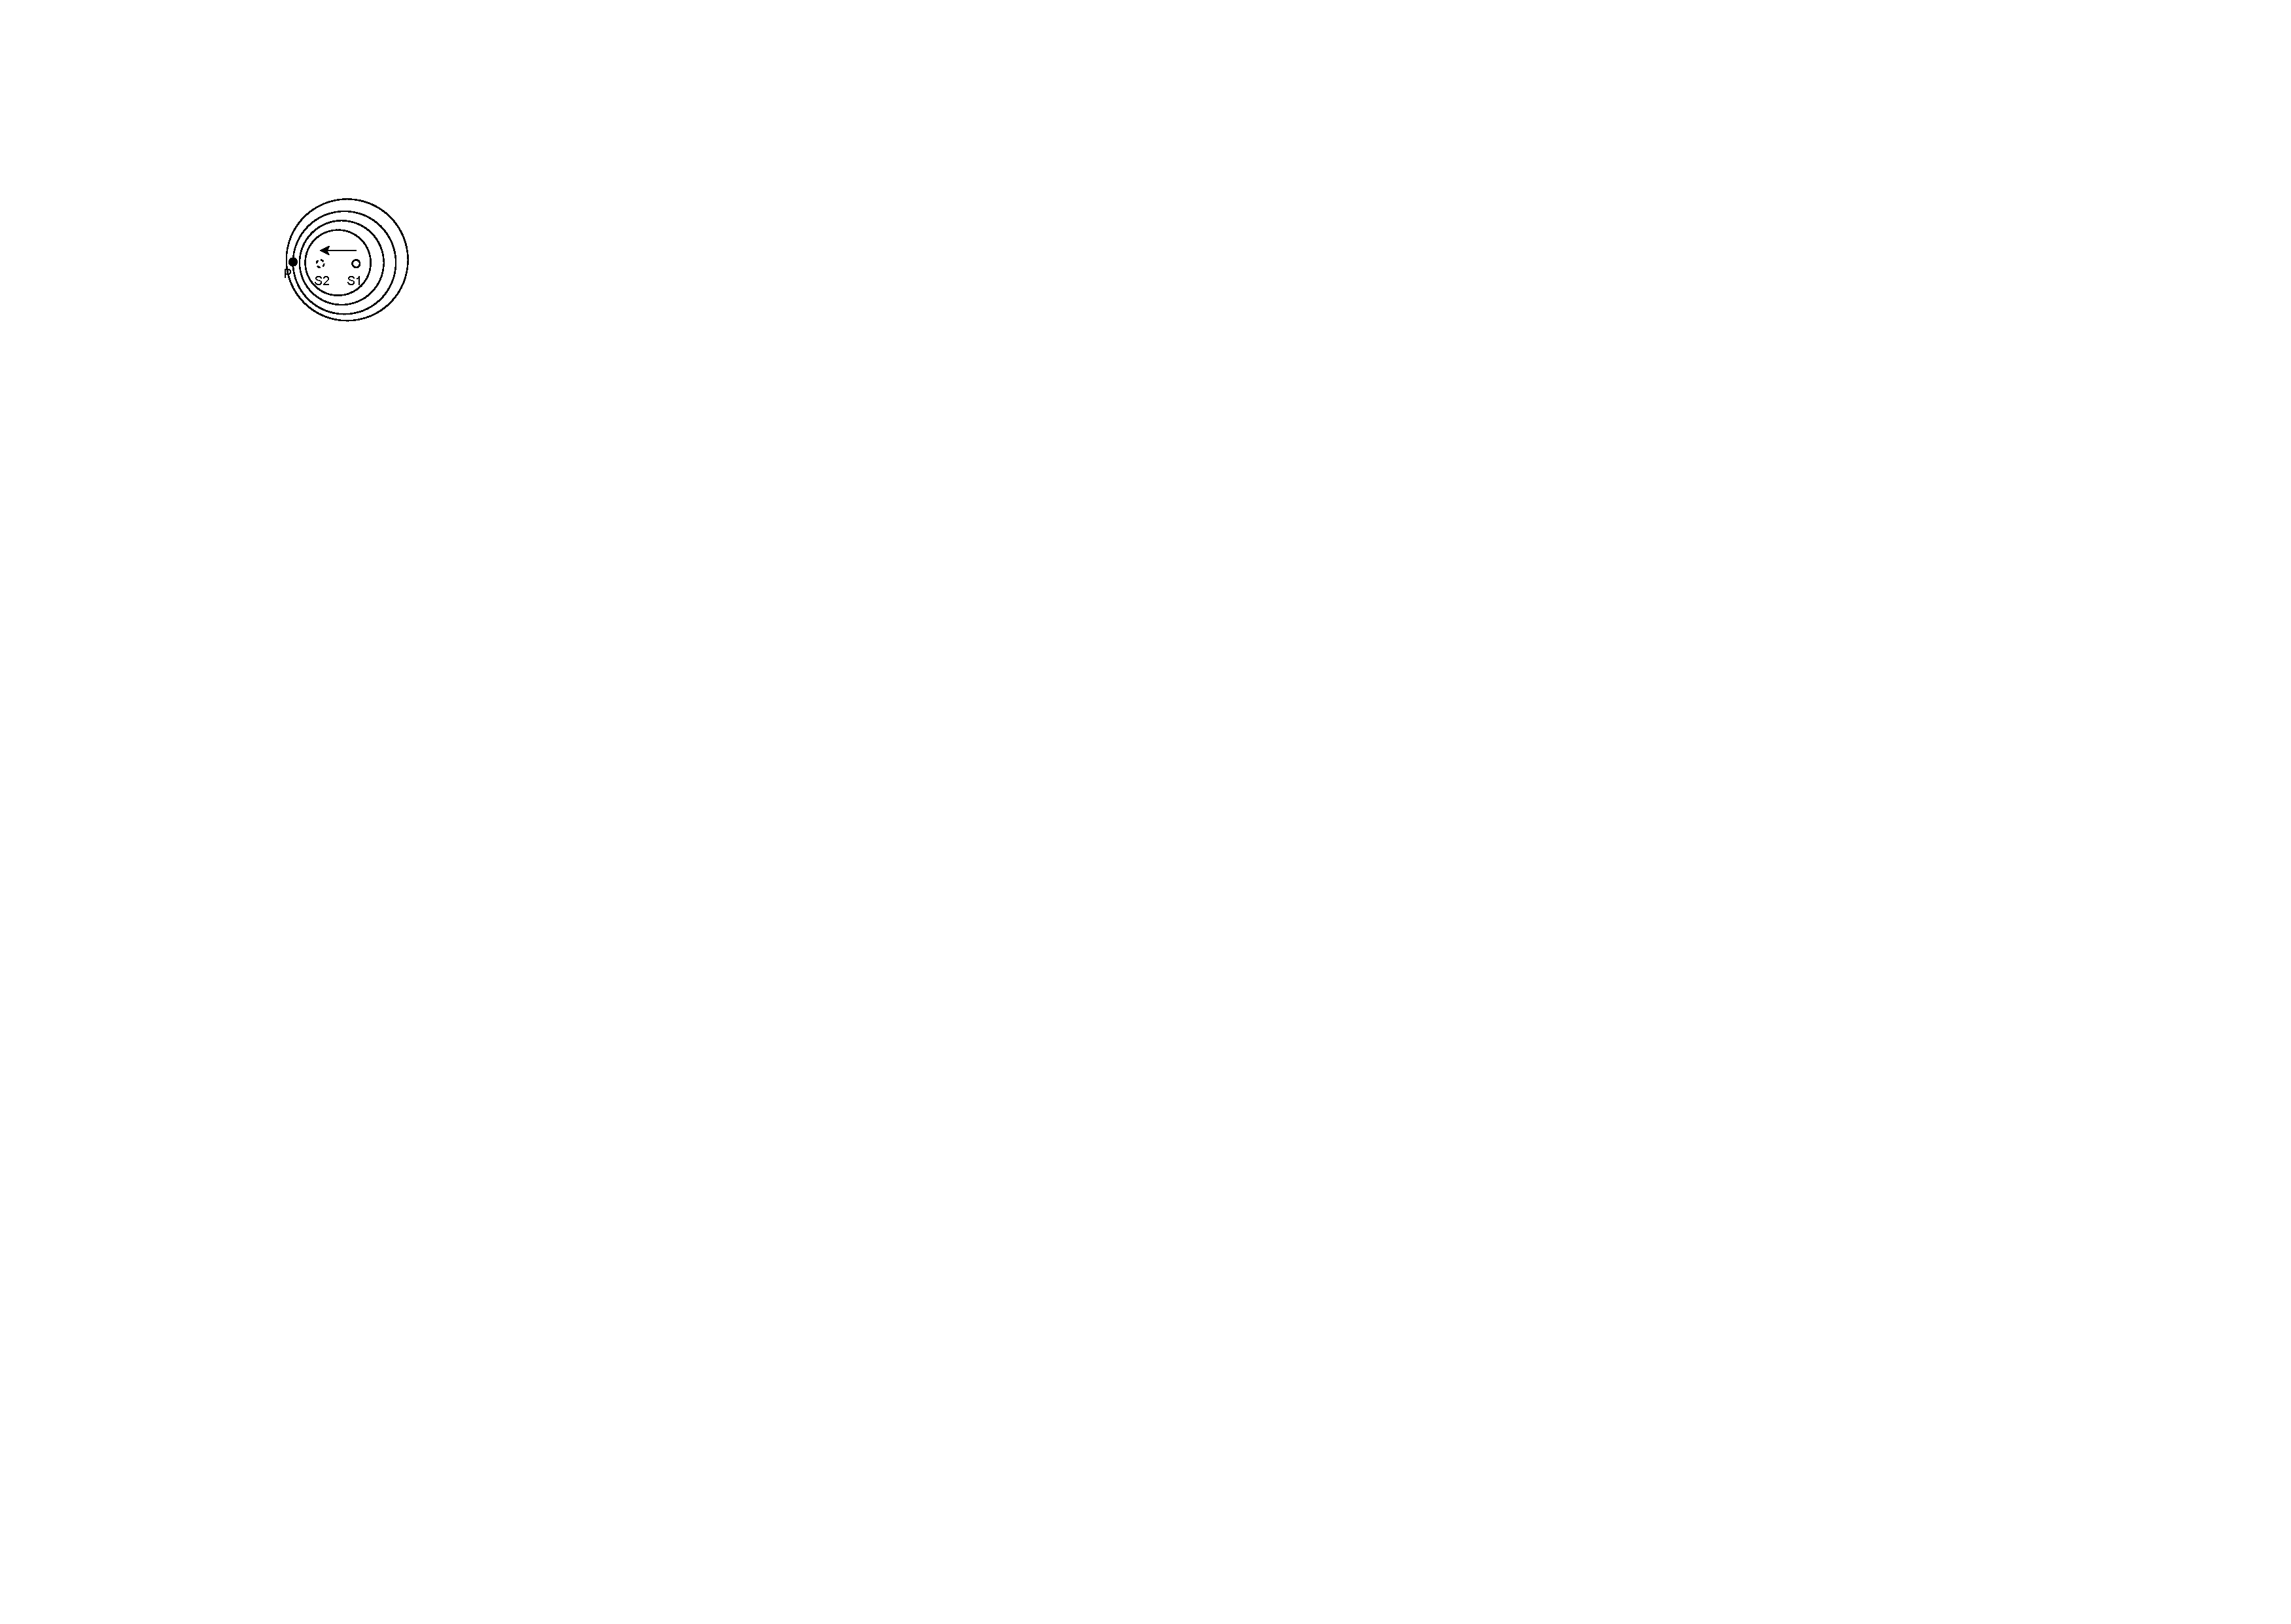
\includegraphics[width=4cm]{fig/2-fig/多普勒频移示意图.drawio.pdf}
    \caption{多普勒频移示意图}
    \label{fig:多普勒频移示意图}
  \end{figure}




由于波源和接收体之间的相对运动而产生的频率变化值的大小与相对运动的速度之间存在定量推导关系,从而使得多普勒频移广泛应用于激光速度/位移测量领域。如图\ref{fig:多普勒频测速示意图}所示,接收体处在\(P\)点,波源从点\(S1\)以速度\(v\)朝着点\(S2\)运动时,有:
\begin{equation}\label{eq:多普勒频测速原理1}
    \Delta L=dcos\theta=v\Delta tcos\theta.
\end{equation}
\begin{figure}[htb]
    \centering
    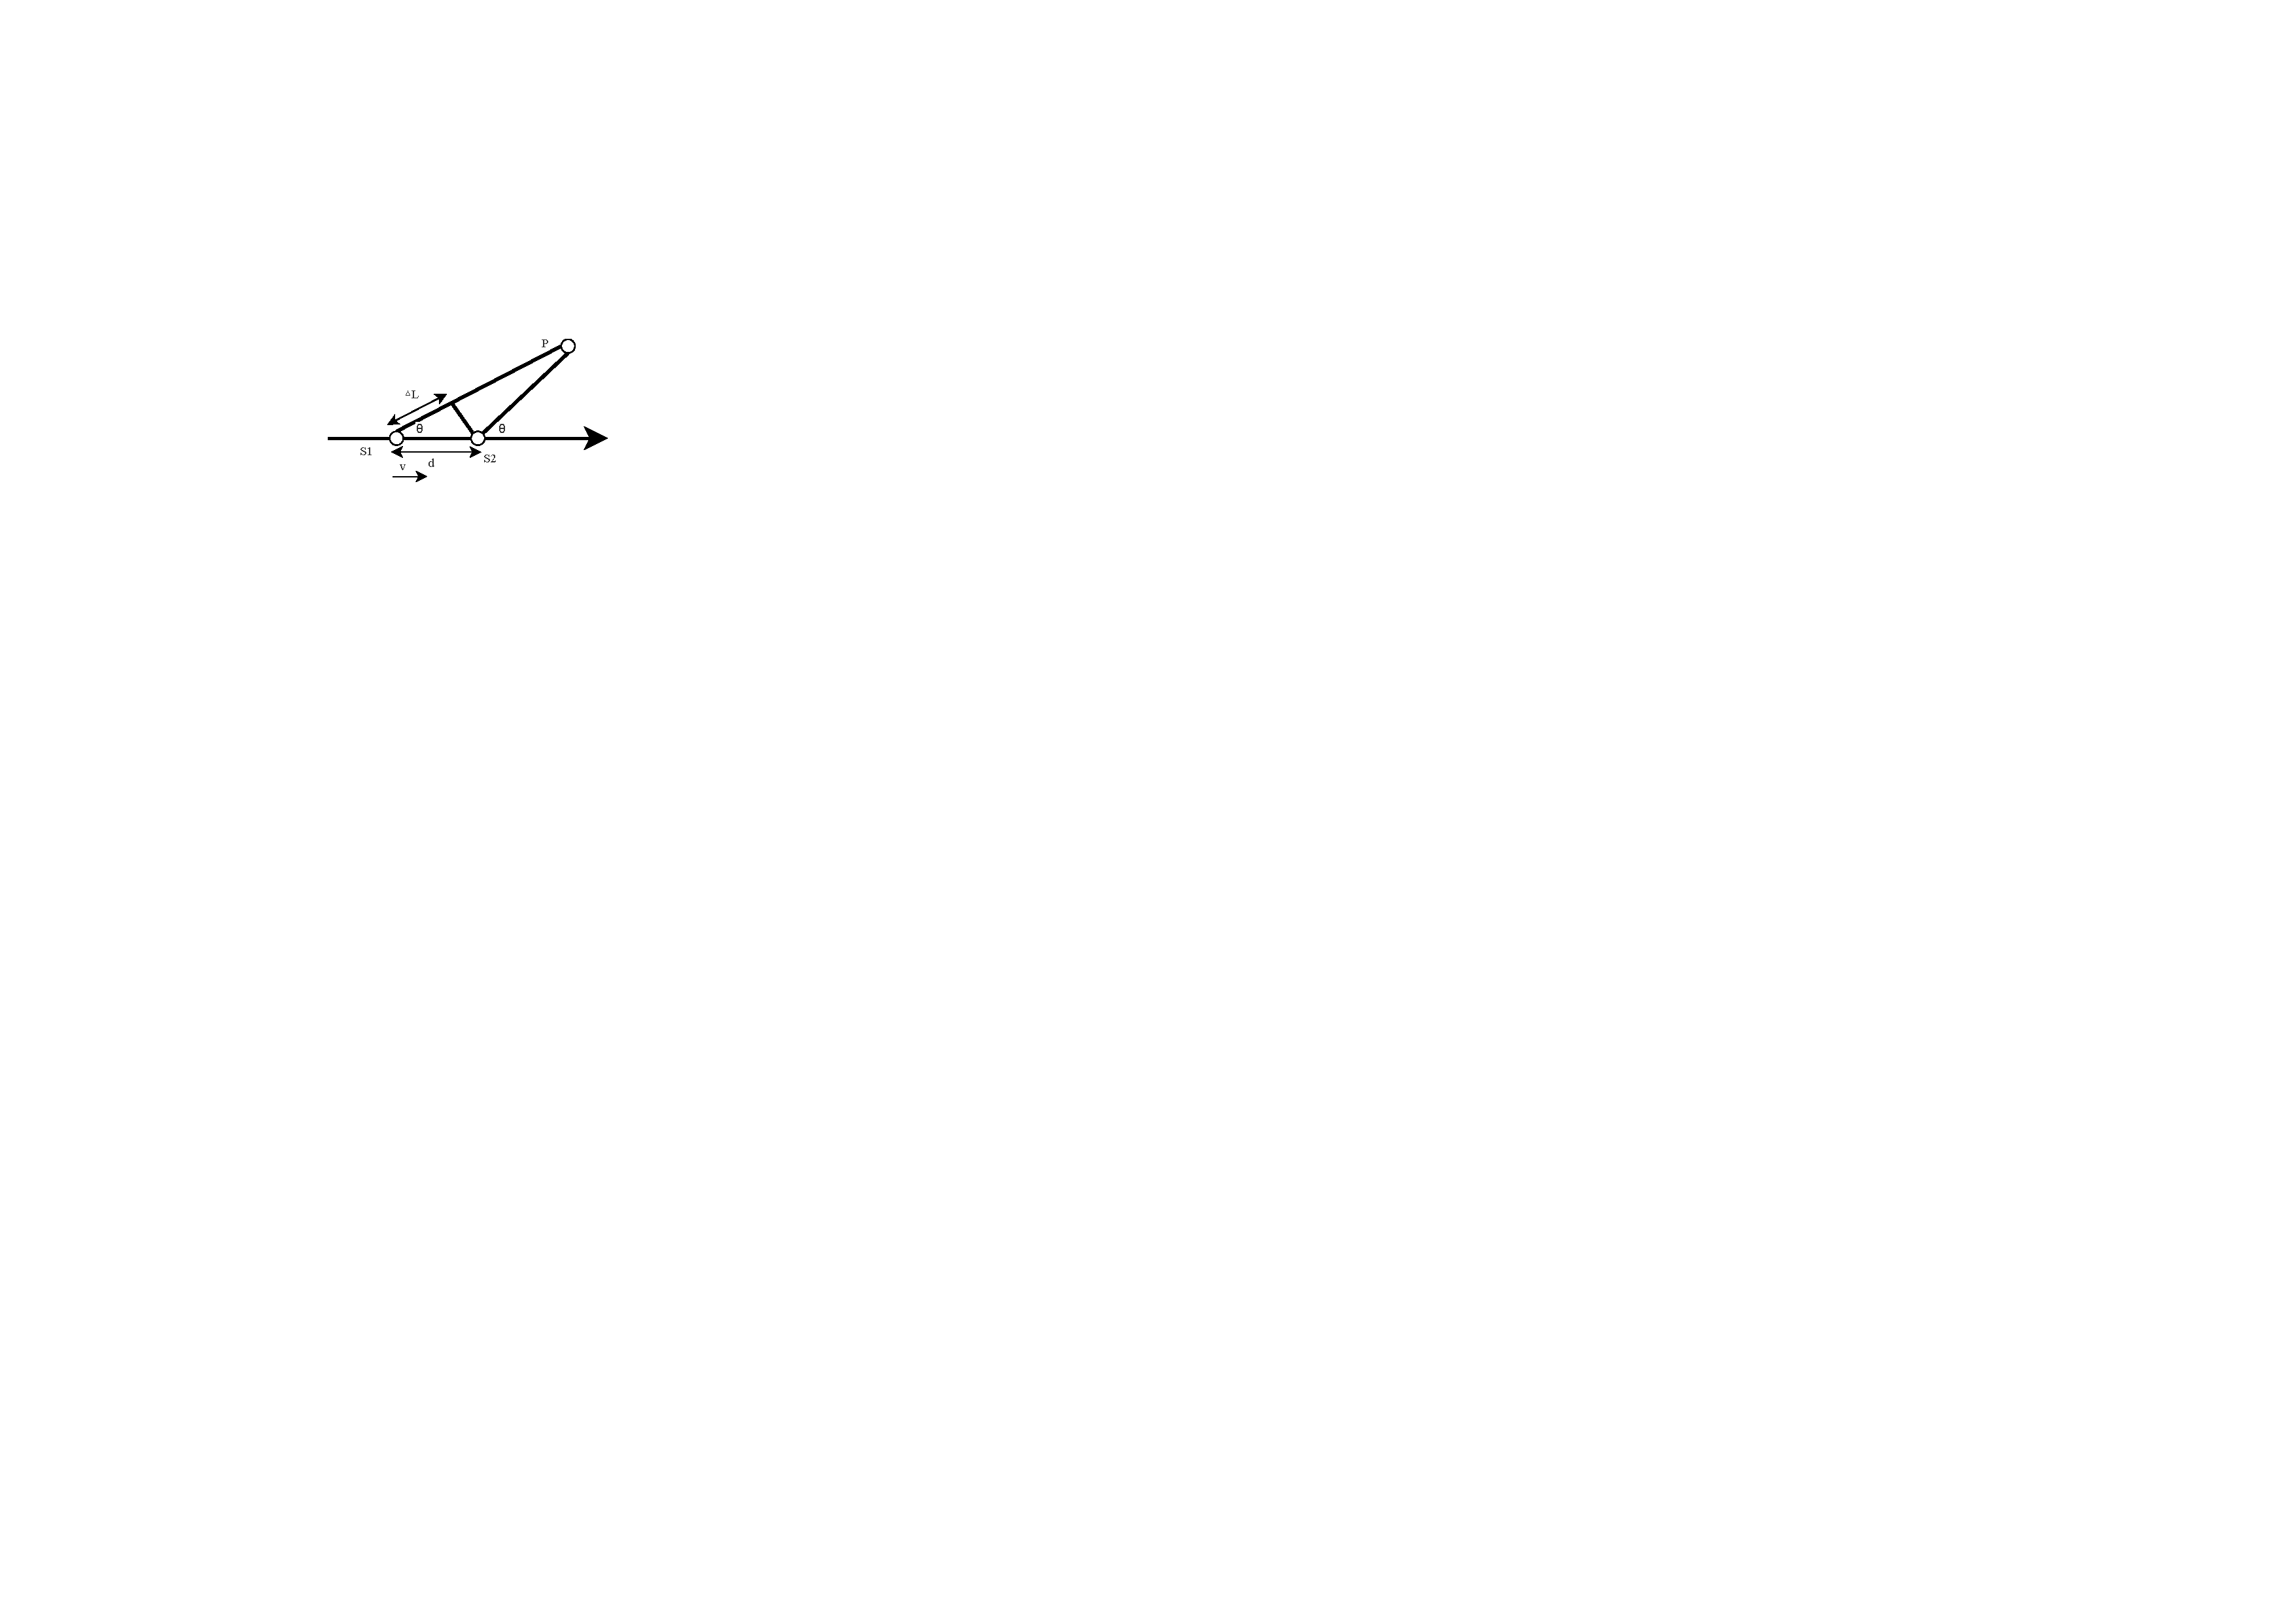
\includegraphics[width=8cm]{fig/2-fig/多普勒频测速示意图.drawio.pdf}
    \caption{多普勒频测速示意图}
    \label{fig:多普勒频测速示意图}
  \end{figure}

式\eqref{eq:多普勒频测速原理1}中\(\theta\)是\(S1\)和\(S2\)处出射波的夹角,\(\Delta L\)两处位置的波程差,\(\Delta t\)为运动所需的时间。由于在实际测量中,波源或者接收体在单位时间内运动距离相比于波源和接收体之间的距离很小,所以可以近似认为\(S1\)和\(S2\)两处的\(\theta\)是相同的\cite{百度百科-多普勒频移},由于波的传播路程差导致的相位变化值为:
\begin{equation}\label{eq:多普勒频测速原理2}
    \varphi=\frac{2\pi \Delta L}{\lambda}=\frac{2\pi v\Delta t}{\lambda}cos\theta.
\end{equation}


对式\eqref{eq:多普勒频测速原理2}左边进行变换,即可得到多普勒频移与运动速度v之间的关系:

\begin{equation}\label{eq:多普勒频测速原理3}
    \varphi_d=\frac{\Delta \varphi}{2\pi \Delta t}=\frac{v}{\lambda}cos\theta.
\end{equation}



\subsection{拍频现象}
对于两个振动方向相同、振动频率相同并且相位差恒定的简谐波叠加,会在空间中产生强弱相间的固定分布,这种现象称为干涉。如若两个简谐波的振动频率略有差异,其叠加时会在空间中产生幅值随时间变化的周期性分布,这种现象则称为拍\cite{基于拍频测量温度和旋光角的方法研究},拍频则定义为单位时间内合振幅周期性强弱变化的次数。

假设两个振动方向相同的简谐波的方程为
\begin{equation}\label{eq:简谐波方程1}
    x_1=A_1cos\omega_1t.
\end{equation}
\begin{equation}\label{eq:简谐波方程2}
    x_2=A_2cos\omega_2t.
\end{equation}

上式中\(A_1=A_2\),并且\(|\omega_1-\omega_2|<<\omega_1+\omega2\),那么\(x_1\)和\(x_2\)在空间中相遇叠加产生的拍的方程为:
\begin{equation}\label{eq:简谐波叠加后方程}
   x=x_1+x_2=2Acos(\omega_1t+\omega_2t).
\end{equation}

对式\eqref{eq:简谐波叠加后方程}进行化简后可以得到:
\begin{equation}\label{eq:化简后简谐波叠加方程}
  x=x_1+x_2=2Acos(\frac{\omega_2-\omega_1}{2}t)cos(\frac{\omega_2+\omega_1}{2}t).
\end{equation}

上式中\(|2Acos(\frac{\omega_2-\omega_1}{2}t)|\)为\(x_1\)和\(x_2\)在空间中叠加后拍的幅值,可以看出这是一个随时间周期性变化的值,而\(\frac{\omega_2+\omega_1}{2}\)则为拍的角频率,这也是一个随着时间周期性变化的值,两者共同导致了拍在波形上表现为周期性变化的形式,如图\ref{fig:拍频波形示意图}所示。
\begin{figure}[htb]
  \centering
  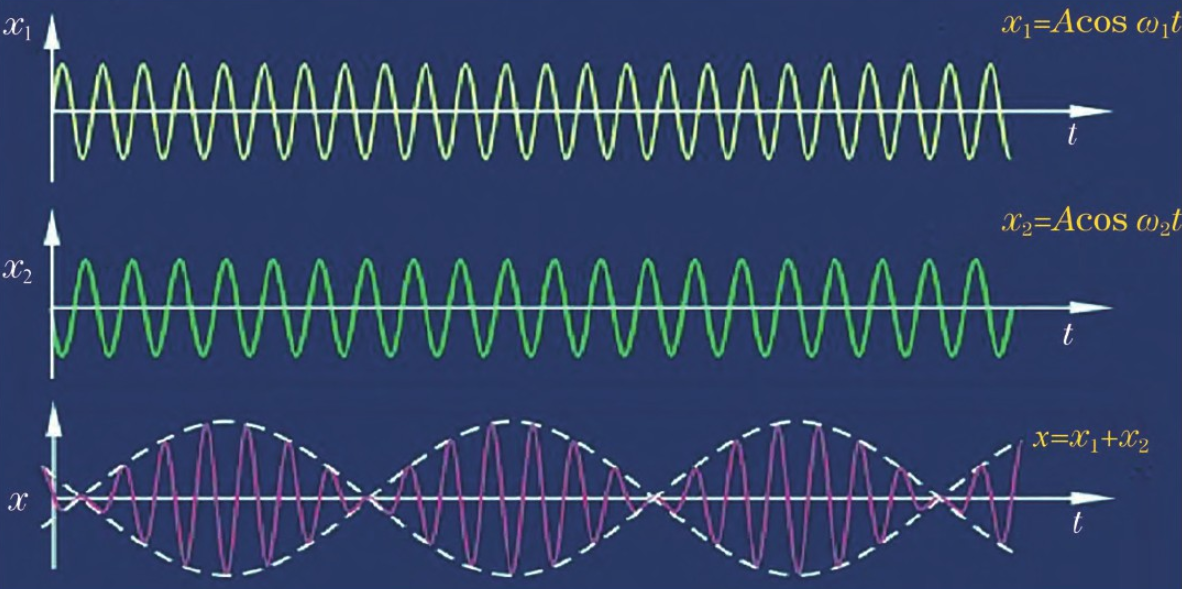
\includegraphics[width=12cm]{fig/2-fig/拍频波形示意图.jpg}
  \caption{拍频波形示意图\cite{张志平2022激光外差干涉技术在光刻机中的应用}}
  \label{fig:拍频波形示意图}
  \end{figure}

并且根据角频率和频率之间的转换关系:\(\omega=2\pi f\)和式\eqref{eq:化简后简谐波叠加方程}可以看出,拍的频率为两个简谐波的原始频率之差的一半,即:
\begin{equation}\label{eq:合成拍与原始简谐波之间的频率关系}
  f=\frac{f_1-f_2}{2}.
\end{equation}

虽然当前激光的频率通常很高(约为\(10^{14}Hz\)量级),这使得目前的光电探测器无法响应\cite{张志平2022激光外差干涉技术在光刻机中的应用},但通过拍频现象,即可将高频的信息转变为低频信息,便于光电探测器响应。

\section{激光干涉仪原理}
\subsection{单频激光干涉仪}
单频激光干涉仪,也可以称为零差干涉仪,具有精度高、稳定可靠, 且相对成本较低等特点\cite{零差干涉仪用于振动校准中关键技术的研究}。其示意图如图\ref{fig:单频激光干涉仪原理图}所示。
\begin{figure}[htb]
    \centering
    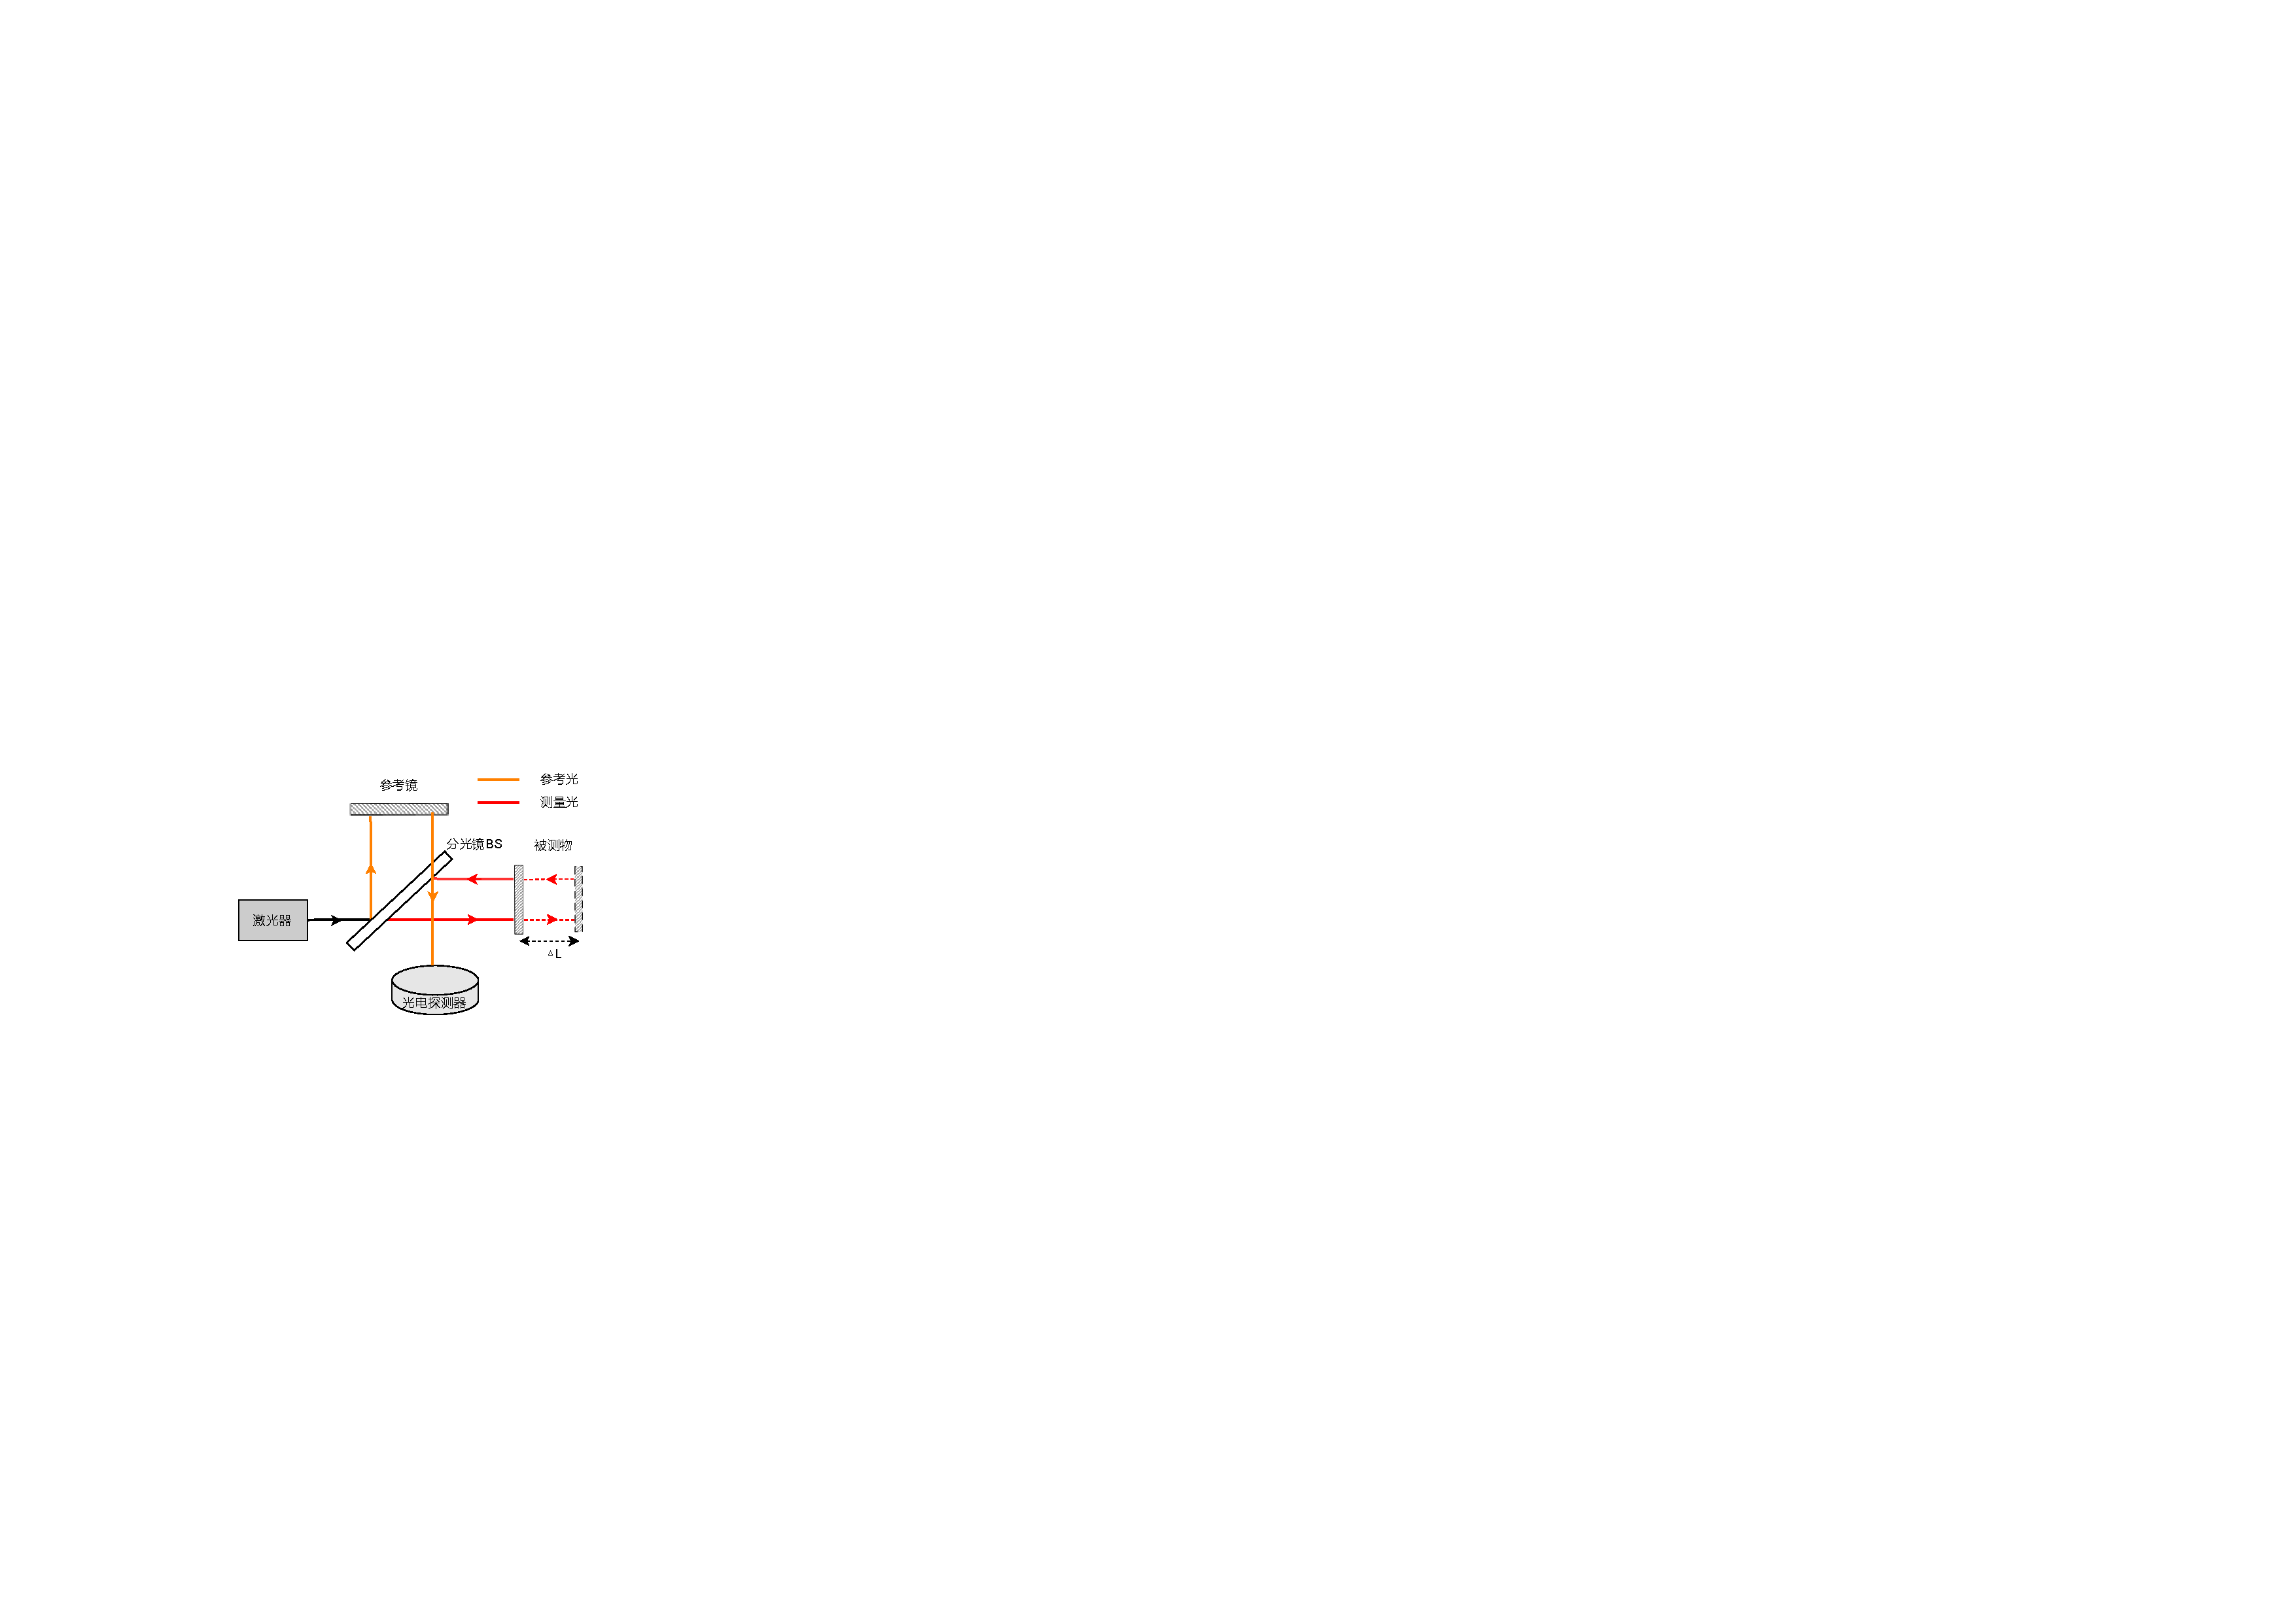
\includegraphics[width=8cm]{fig/2-fig/单频激光干涉仪原理图.drawio.pdf}
    \caption{单频激光干涉仪原理图}
    \label{fig:单频激光干涉仪原理图}
\end{figure}

激光器出射的激光经过分光镜BS后产生两束光:一束进入参考臂,并被参考镜反射,另一束进入测量臂,并被被测物体反射,当被测物体位移为\(\Delta L\)时,测量光会携带上对应的多普勒频移\(f_d\),两束光分别经参考镜和被测物体反射后会再次汇聚,随后射入光电探测器,根据相位的变化即可反推被测物体的位移。

\subsection{双频激光干涉仪}
双频激光干涉仪结构如图\ref{fig:双频激光干涉仪原理图}所示,激光出射的含有\(f_1\)和\(f_2\)两个频率成分的激光经过偏振分光棱镜(polarization beam splitter,PBS)分为测量光\(f_1\)和参考光\(f_2\),测量光\(f_1\)进入测量臂之后,携带上被测物体位移\(\Delta L\)的多普勒频移\(\Delta f\)。由于测量臂和参考臂上各放置了一块四分之一玻片(Quarter Wave Plate,QWB),测量光和参考光在返回PBS之前都经过两次QWB,使得其偏振态发生改变,原本透射的测量光再次返回PBS时变为反射,原本反射的参考光再次返回PBS时变为透射,参考光和测量光汇聚,耦合进光纤,由采集板卡从多普勒频移\(\Delta f\)解调出被测物体的位移\(\Delta L\)。
\begin{figure}[htb]
    \centering
    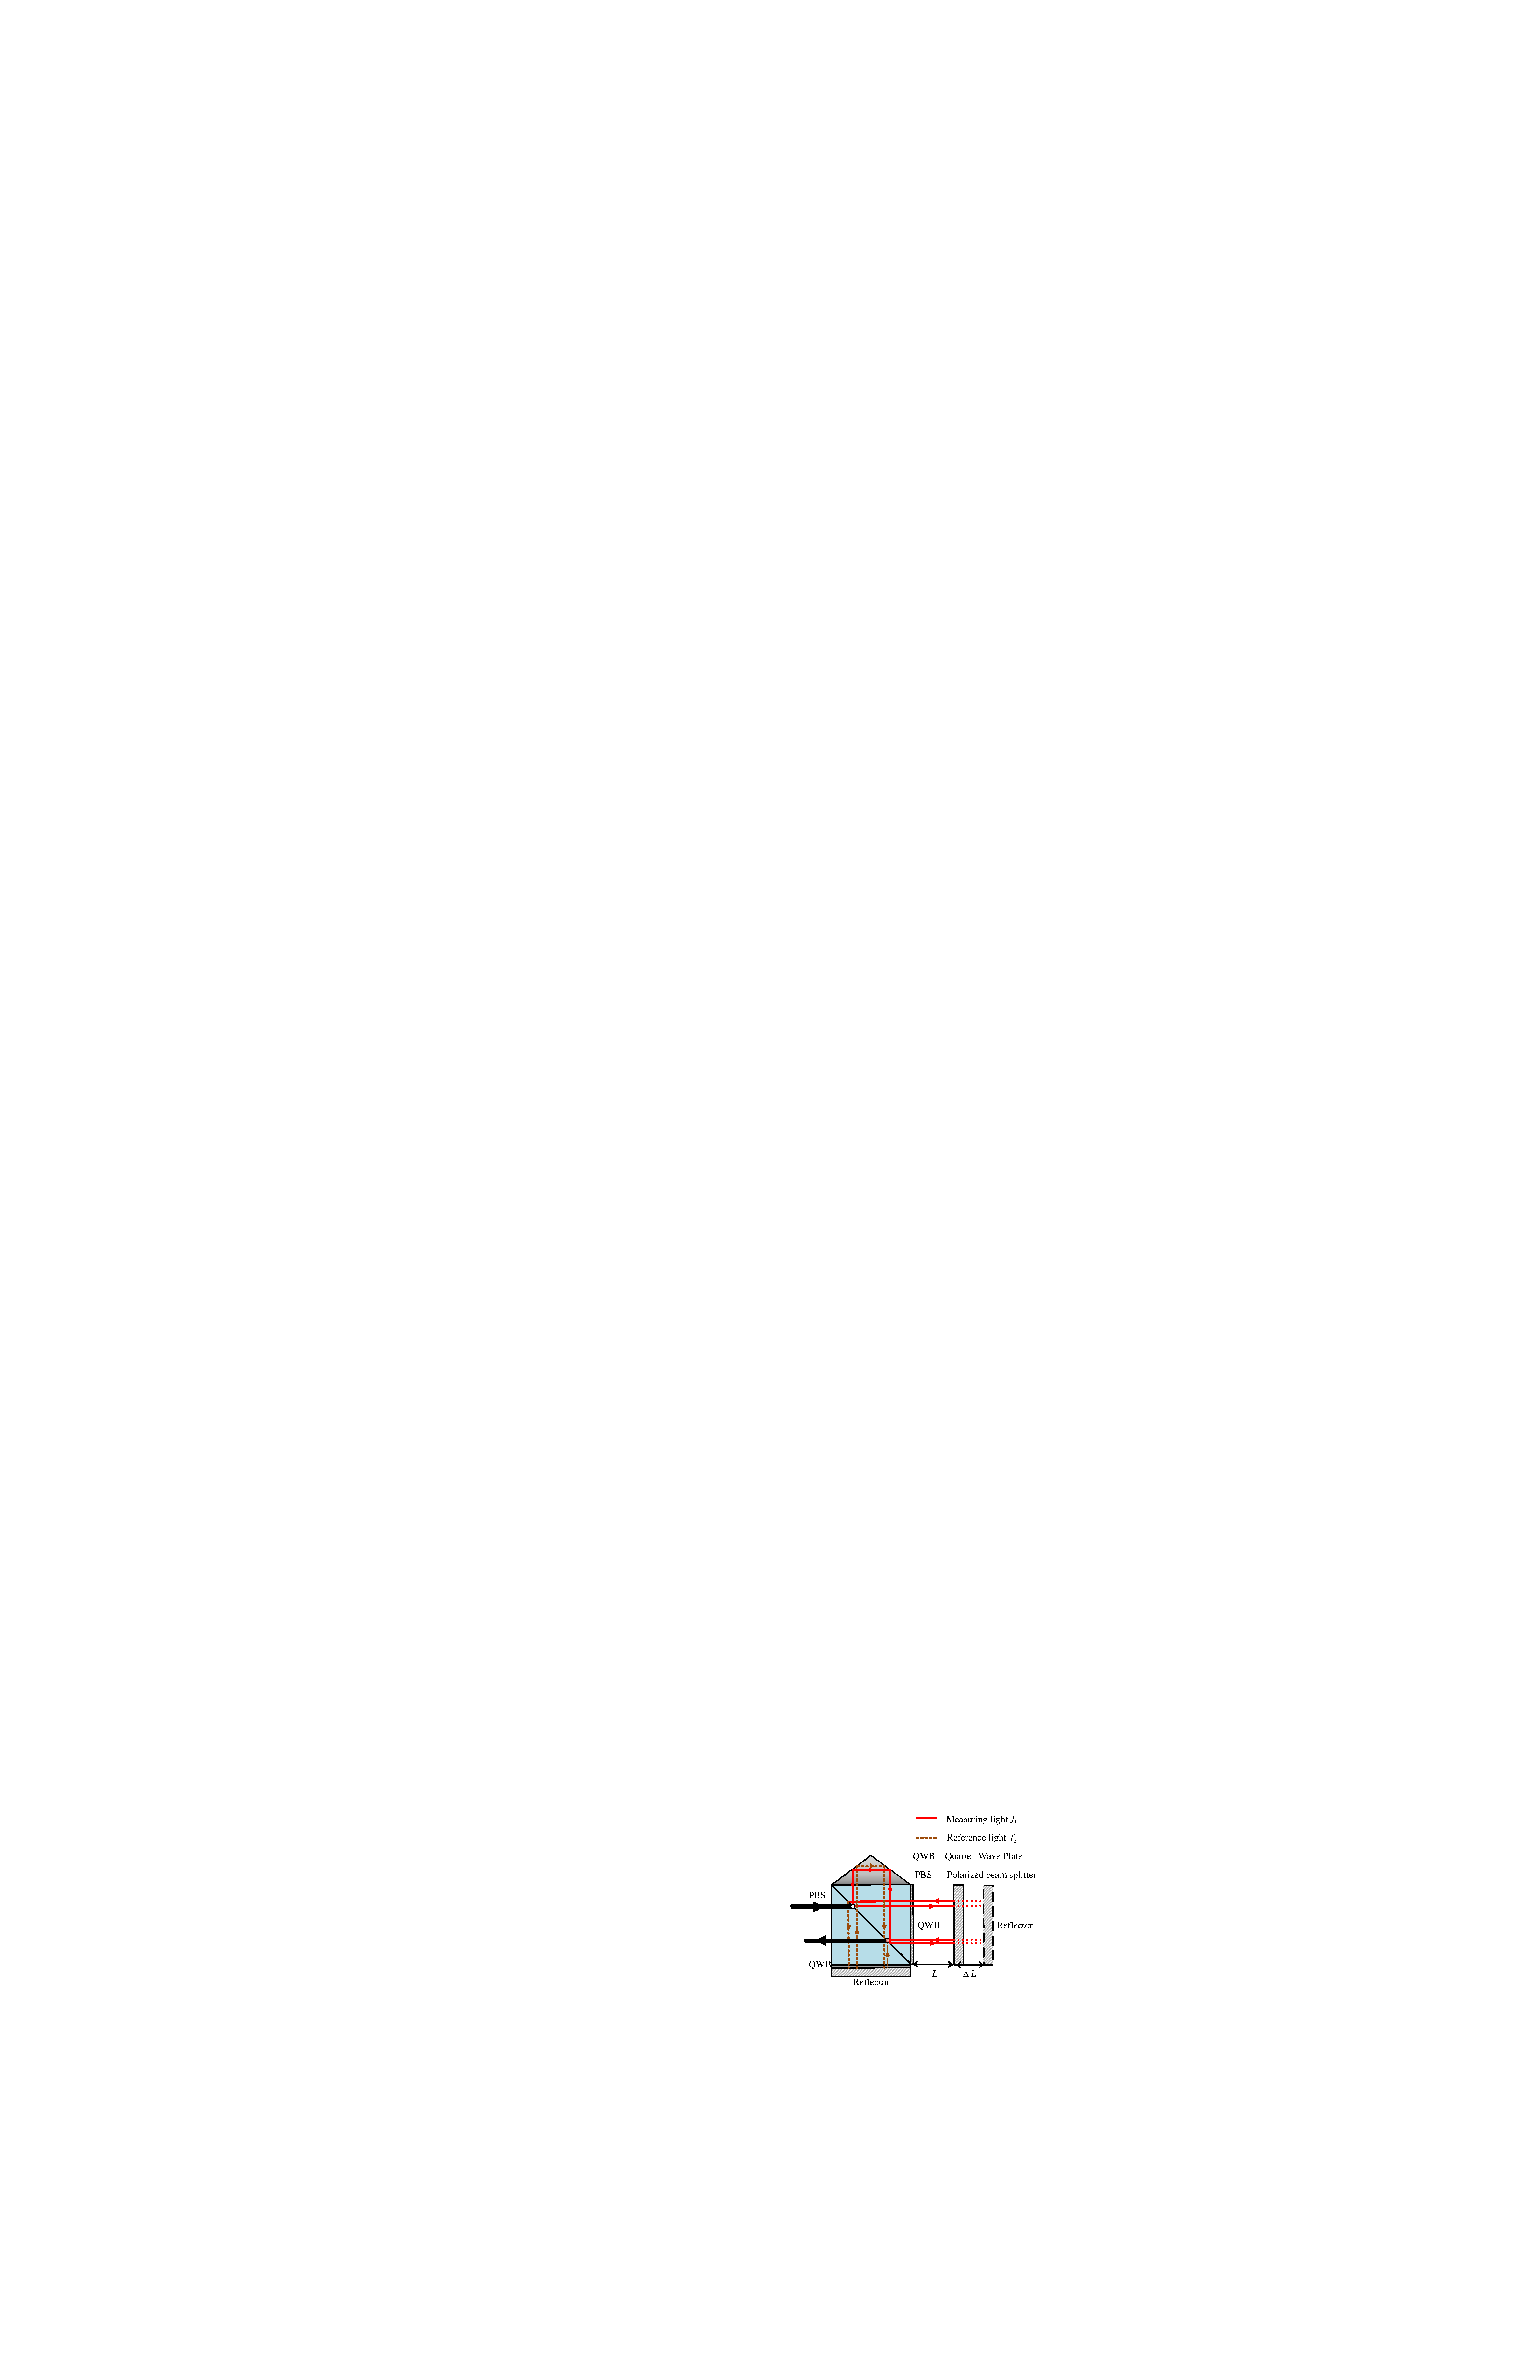
\includegraphics[width=9cm]{fig/2-fig/双频激光干涉仪原理图.pdf}
    \caption{双频激光干涉仪原理图}
    \label{fig:双频激光干涉仪原理图}
\end{figure}

从图\ref{fig:双频激光干涉仪原理图}可以看出,激光从激光器出射后经过一次反射才达到接收体,不同于图\ref{fig:多普勒频测速示意图}中波源直接抵达接收器的情况,所在双频激光干涉仪中物体移动的距离应是两倍的影响,即式\eqref{eq:多普勒频测速原理1}应乘2,并且一般都为垂直入射,所以\(\theta\)可近似认为0,所以式\eqref{eq:多普勒频测速原理3}可改写为:
\begin{equation}\label{eq:干涉仪中多普勒相位}
  \varphi_d = \frac{2v}{\lambda}.
\end{equation}

并且由于\(v=dl / dt\),带入式\eqref{eq:干涉仪中多普勒相位}中可得:
\begin{equation}\label{eq:干涉仪中多普勒位移微分}
  dl = vdt = \frac{\lambda}{2}\Delta f dt.
\end{equation}

上式中\(dl\)被测物体单位时间内的位移,即位移的微分量,\(\Delta f\)为\(dl\)对应的多普频移,对式\eqref{eq:干涉仪中多普勒相位}进行积分可得:
\begin{equation}\label{eq:干涉仪中多普勒积分}
  L = \int_{0}^{t} vdt =\int_{0}^{t} (\frac{\lambda \Delta f}{2})dt = \frac{N\lambda}{2}.
\end{equation}

式\eqref{eq:干涉仪中多普勒积分}即为双频激光干涉仪位移测量的基本公式\cite{丁子婷双频激光干涉仪测量系统的环境误差研究}。

\section{双频激光干涉仪的环境误差及其成因}
但在真实的测量场景中,双频激光干涉仪的测量值\(D\)是指干涉仪系统实际输出的位移值。是由条纹数\(N\)乘上干涉仪系统的分辨率\(R_{es}\)得到的,而条纹数\(N\)与光程的变化有光,即:
\begin{equation}\label{eq:测量值与光程的关系}
    D=R_{es}{\times}N=R_{es}{\times}\frac{\Delta L{\times}n_0{\times}M_o}{\lambda{\div}M_e}=\Delta L{\times}n_0.
\end{equation}

式\eqref{eq:测量值与光程的关系}中,\(n_0\)为真空中的空气折射率,近似可认为1,干涉仪的分辨率\(R_{es}\)与激光的实际波长\(\lambda\)、电子细分\(M_e\)和光学细分\(M_o\)有关。电子细分\(M_e\)由干涉仪系统的采集板卡决定,常见的有32、64、128、256......2048等,而光学细分\(M_o\)只与干涉仪的设计结构有关,对于采用角锥镜为被测对象的干涉仪,光学细分一般为2,采用平面镜为被测对象的干涉仪,光学细分一般为4,干涉仪的分辨率具体计算公式如下:
\begin{equation}\label{eq:分辨率与细分的关系}
    R_{es}=\frac{\lambda}{M_o{\times}M_e}.
\end{equation}

电子细分和光学细分在测量过程中一般不会引入太大的误差,但是激光的波长跟测量环境中的空气折射率有关,而外界环境因素(温度、气压等)的变化也会导致空气折射率变化\(\Delta n\),此时,干涉仪系统测量值\(D\)不仅包括被测物体的位移\(\Delta L\),还包括由于折射率变化引起的光程变化\(\Delta l\),即:
\begin{equation}\label{eq:实际的位移公式}
    D=\Delta L(\Delta n+n_0)+L\Delta n.
\end{equation}

但由于测量臂长度\(L\)一般远大于被测物体位移\(\Delta L\),由式\eqref{eq:测量值与光程的关系}和式\eqref{eq:实际的位移公式}可得,由于外界环境因素(温度、气压等)引起的误差为:
\begin{equation}\label{eq:环境误差公式}
    D=[\Delta L(\Delta n+n_0)+L\Delta n]-\Delta Ln_0=\Delta n(\Delta L+l) \approx \Delta n \Delta L.
\end{equation}

根据相关文献的描述\cite{徐建2013双频激光干涉仪系统线性测量误差主要来源及减小误差的方法分析},在对上述环境因素不进行任何控制或补偿的情况,空气折射率的变化可能会达到50ppm,如果仅对测量环境温度进行控制,其余因素的变化也可能导致空气折射率变化20ppm以上。放在双频激光干涉仪领域,根据式\eqref{eq:环境误差公式}可知,空气折射率变化需要乘上测量臂长度才是双频激光干涉仪的环境误差,这就导致当测量臂长度较小时,这部分的误差是可以忽略不计的,但随着测量臂长度的增加,双频激光干涉仪的环境误差也随着增大。以10mm的测量臂长度为例,当温度变化超过\(0.1\)$^{\circ}$C时,这部分的误差就可能已经超过1nm了,所以需要对上述的环境误差进行补偿。

\section{基于Edlen公式的补偿方法及其局限性}
\subsection{Edlen公式补偿方法}
1965年,Edlén基于洛伦兹方程和空气密度方程推导出了空气密度因子,并基于空气密度因子提出Edlen公式用于空气折射率的修正\cite{2015Refractive}。最近一次广泛承认的修正是Boensch等\cite{1998Fit}于1998年优化的Edlen公式,其中关于空气折射率与温度和气压的关系如式\eqref{eq:原始Edlen公式}所示。
    \begin{equation}\label{eq:原始Edlen公式}
    (n\,-\,1)_{tp}=\frac{Pn_0}{93214.60}\frac{[1\,+\,10^{-8}(0.5953\,-\,0.009876T)]}{1\,+\,0.0036610T}.
    \end{equation}

式\eqref{eq:原始Edlen公式}中 \((n-1)_{tp}\)为考虑温度与气压时的空气折射率,\(n_0\)为理想情况下空气折射率,\(P\)为环境气压,\(T\)为环境温度。当气压\(P\)取一个标准大气压(101.325\(kPa\)),温度\(T\)从\(20\)$^{\circ}$C变化到\(30\)$^{\circ}$C时,折射率随温度的变化如图\ref{fig:折射率-温度}所示;当温度\(T\)取\(20\)$^{\circ}$C,而气压\(P\)在一个标准大气压附近变化时,折射率随着气压的变化如图\ref{fig:折射率-气压}所示。
\begin{figure}[htb]
    \centering
    \subfigure[折射率随温度变化]{
      \begin{minipage}[b]{0.70\textwidth}
        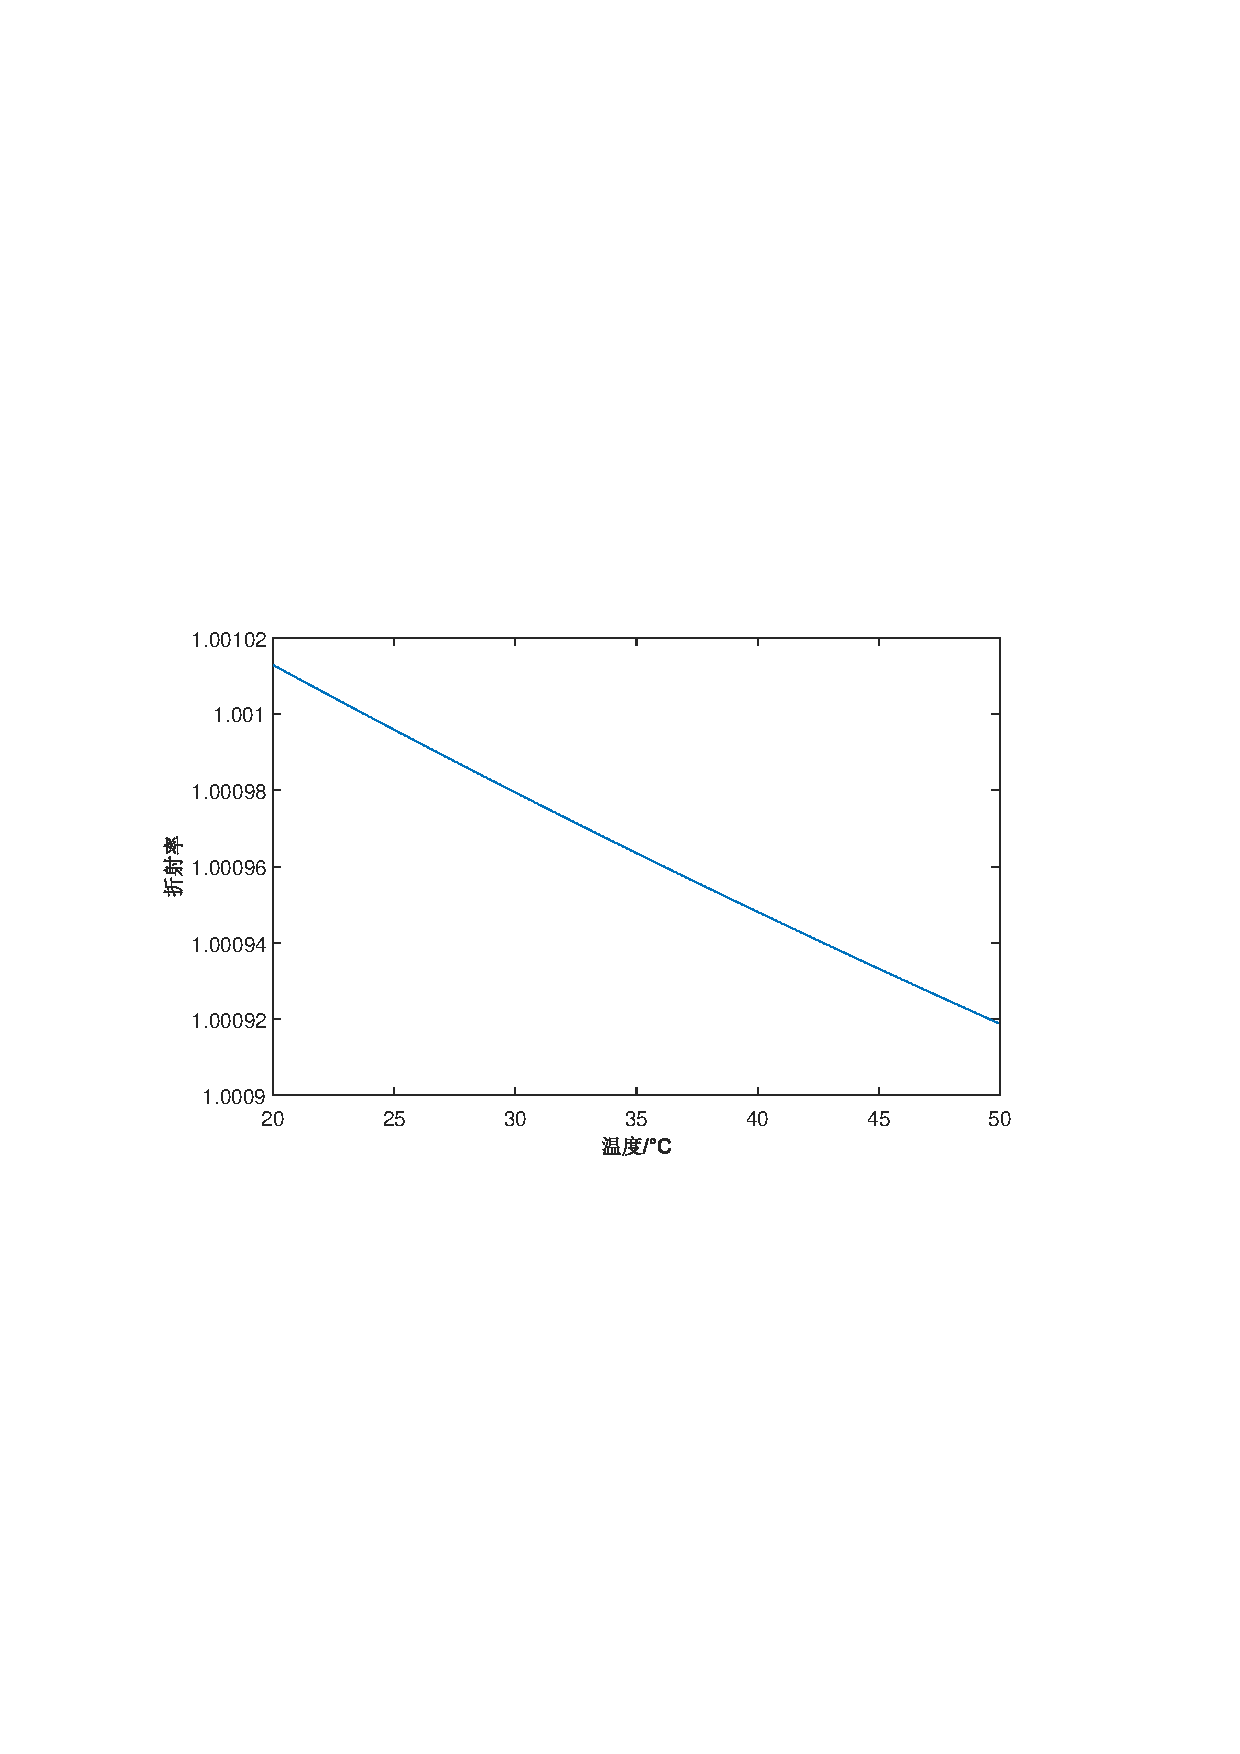
\includegraphics[width=10cm,height=5cm]{fig/2-fig/折射率随温度变化.pdf}
      \end{minipage}
      \label{fig:折射率-温度}
    }
    \subfigure[折射率随气压变化]{
      \begin{minipage}[b]{0.70\textwidth}
        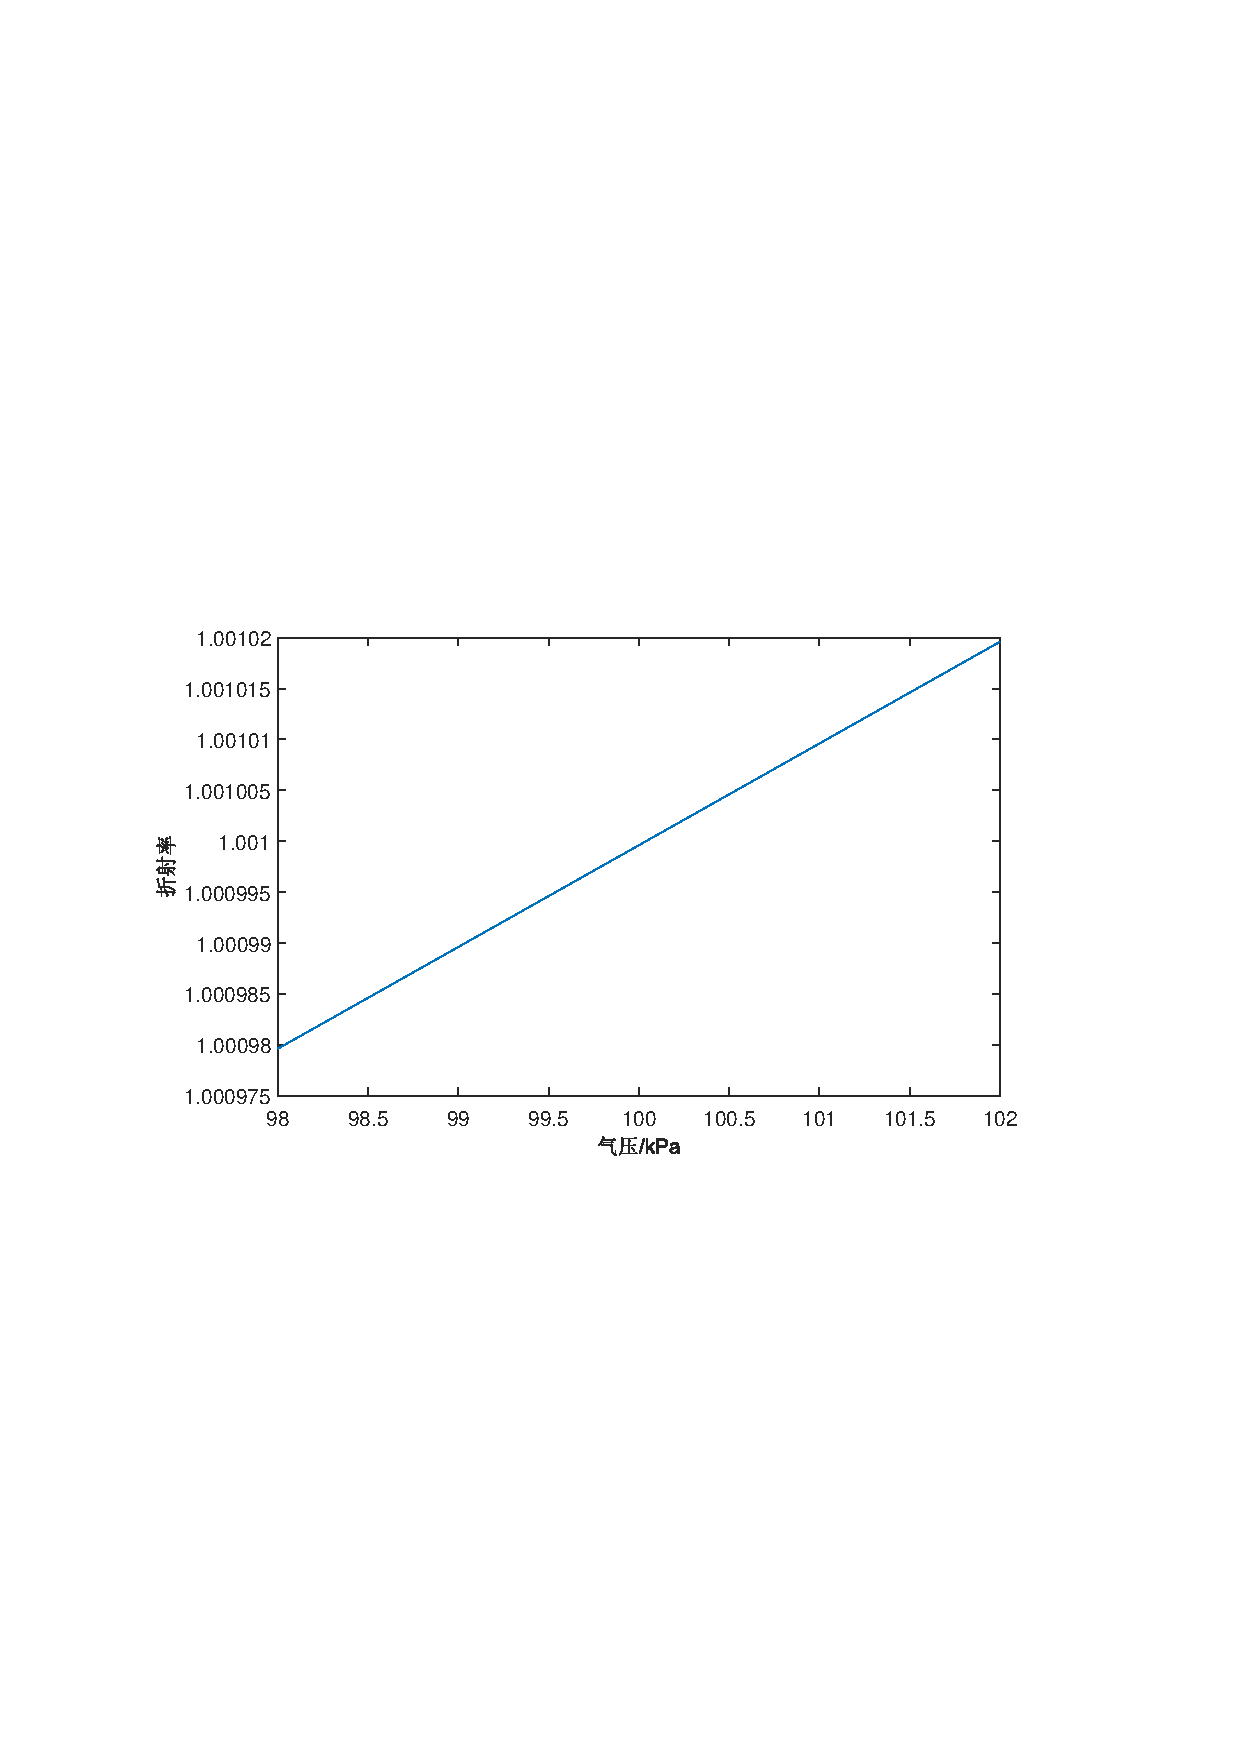
\includegraphics[width=10cm,height=5cm]{fig/2-fig/折射率随气压变化.pdf}
      \end{minipage}
      \label{fig:折射率-气压}
    }
    \caption{折射率变化图}
    \label{fig:折射率变化图}
  \end{figure}

可以看出,在上述范围内,空气折射率和温度/气压变化呈近似线性\cite{李博2021温度对激光干涉法测量气体动态压力的影响}。对式\eqref{eq:原始Edlen公式}中各因子求偏导数,可以得到空气折射率变化\(10^{-8}\)时温度和气压的变化因子分别为\(3.73Pa\)和\(0.01\)$^{\circ}$C\cite{2015Approach}。通过仿真分析,可得出温度和气压对空气折射率的影响呈线性或近线性关系,\eqref{eq:原始Edlen公式}可简化如下\cite{elden公式法在双频激光干涉仪测量系统的应用}:
\begin{equation}\label{eq:线性形式的Edlen公式}
    \Delta n=\frac{\partial n}{\partial T}\,\Delta T+\frac{\partial n}{\partial P}\,\Delta P
    =-9.36*10^{-7}\Delta T\,+\,2.68*10^{-9}\Delta P.
    \end{equation}

式\eqref{eq:线性形式的Edlen公式}中\(\Delta n\)为空气折射率的变化值,\(\Delta T\)为温度变化值,单位为$^{\circ}$C,\(\Delta P\)为气压变化值,单位为\(Pa\)。由温度传感器和压力传感器测量出对应的温度值和压力值,带入式\eqref{eq:线性形式的Edlen公式}计算出空气折射率变化值,再由式\eqref{eq:环境误差公式}即可求出干涉仪的环境误差。
\subsection{局限性}
现有的Edlen公式用于干涉仪环境补偿有着如下局限性:
\begin{enumerate}
  \item 波长不匹配:现有的Edlen公式是根据644.0nm、508.7nm、480.1nm和467.9nm四个波长段的测量数据得出的\cite{2020Effect},而干涉仪由于对光束横模模式和频率稳定性的高要求,所用的激光光源多为波长段为633nm的氦氖激光器,两者在波长段上并不匹配。
  \item 温度不匹配:现有的Edlen公式的适用温度位标准条件下温度20$^{\circ}$C\cite{2020Effect},而干涉仪广泛使用于光刻机中或其它超精密测量领域,其工作环境温度大多为22$^{\circ}$C或常温范围(24$^{\circ}$C-26$^{\circ}$C)。
  \item 主观性强:有的Edlen公式是根据实验数据人为总结的,带有很大的主观性。
\end{enumerate}


\section{本章小结}
本章主要介绍了激光位移测量的基本理论和干涉仪环境误差的成因及Edlen公式补偿方法。首先阐述了激光位移测量领域广泛利用的两个原理:多普勒频移和拍频。随后介绍了单频激光干涉仪和双频激光干涉仪结构和光路,并从双频激光干涉仪一些参数值说起,其中包括分辨率、电子细分、光学细分等,详细分析了环境误差的成因以及影响大小。最后介绍了目前广泛应用于双频激光干涉仪环境误差补偿的Edlen公式,并说明当前Edlen公式存在着波长不匹配、温度不匹配、主观性强三个局限性,为后文的工作提供了基础。
  \chapter{双频激光干涉仪的环境误差补偿实验系统}
\section{双频激光干涉仪测量系统光路设计与分析}
\section{基于PT100的八通道温度测量系统}
本文工作所采用的温度传感器为基于PT100电阻的多通道温度测量系统,最多支持8个通道的同时测量,供电电压为\(+12 \sim +24VDC\),能够支持\(22^{\circ}C \pm 5^{\circ}C\)范围内的温度测量,测量精度\(\leq \pm 0.04^{\circ}C\)。
\subsection{上位机系统}
基于PT100电阻的多通道温度测量系统上位机采用美国国家仪器(NI)公司研制开发的LabVIE程序开发环境开发,并且需要NI LabVIEW Runtime和NI-VISA模组。该上位机软件能够实现数据的测量、显示、存储并且自带标定数据分析功能,包含main.vi一个主vi以及数据处理.vi和数据存储.vi两个子vi,上位机软件流程图以及部分关键代码如图\ref{fig:上位机程序示意图}所示。
\begin{figure}[htb]
    \centering
    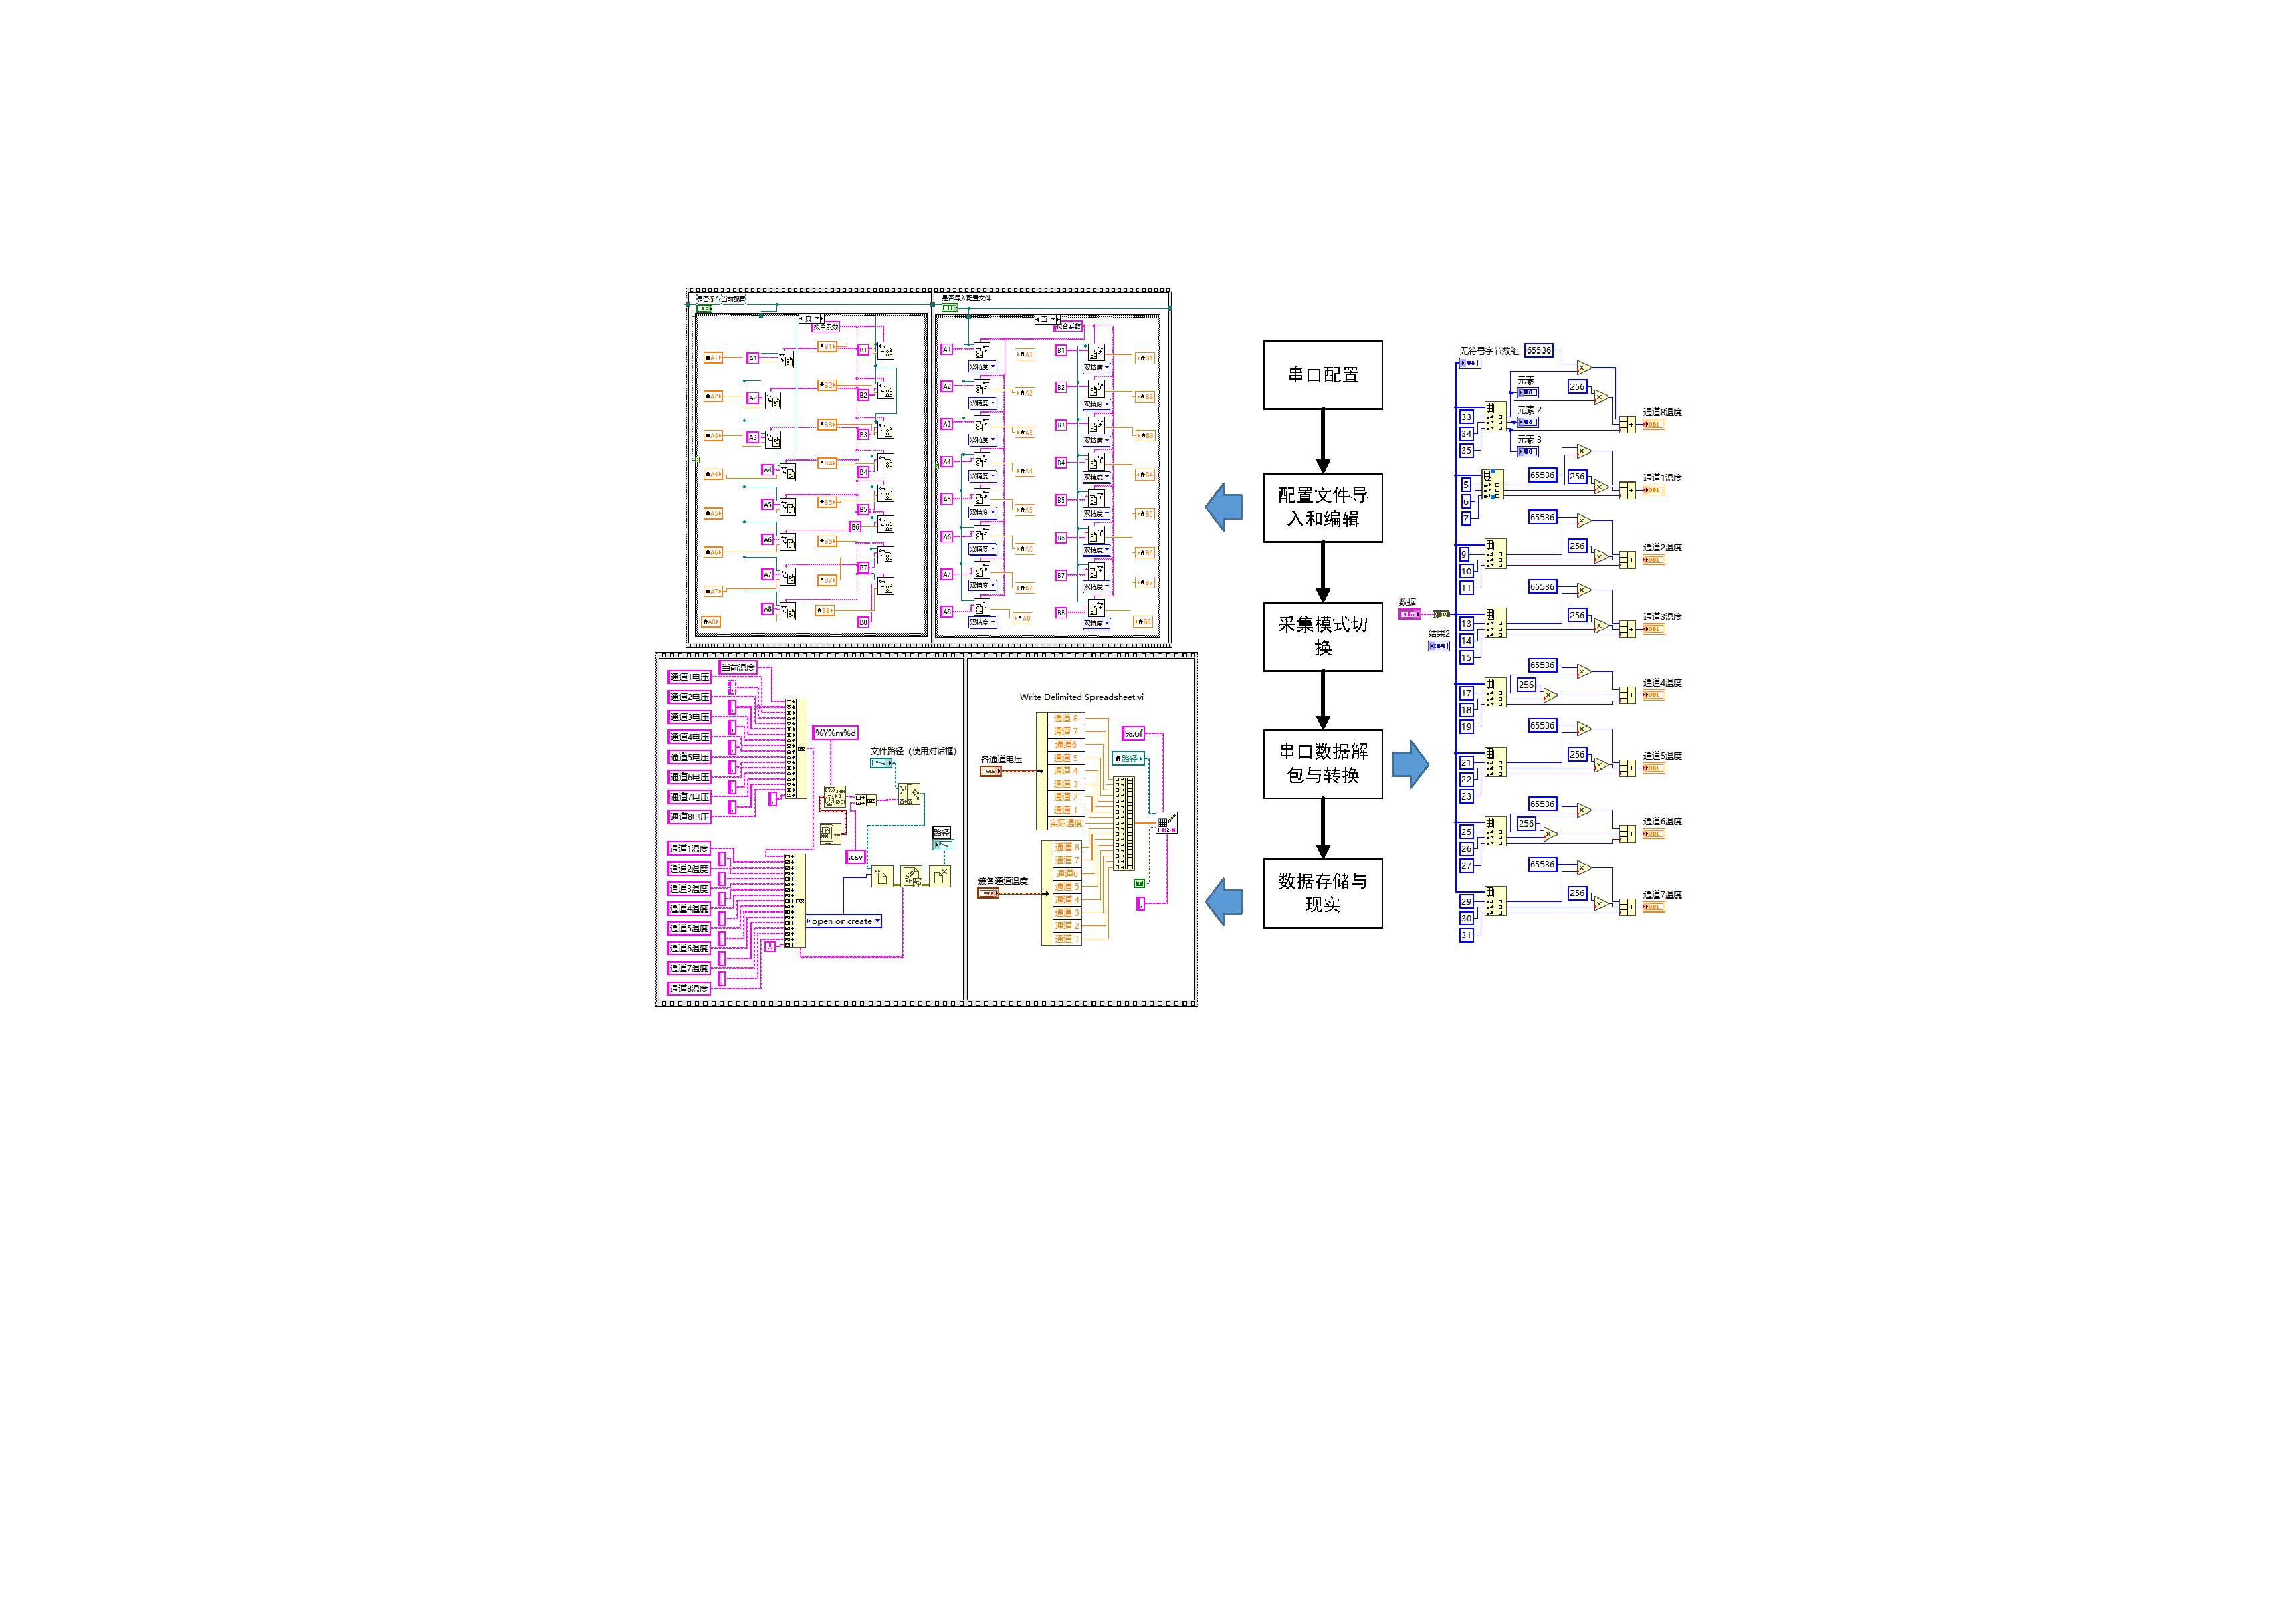
\includegraphics[width=14cm]{fig/3-fig/上位机程序示意图.pdf}
    \caption{上位机程序示意图}
    \label{fig:上位机程序示意图}
\end{figure}

程序的面向用户界面如图\ref{fig:温度测量上位机前面板}所示:
\begin{figure}[htb]
    \centering
    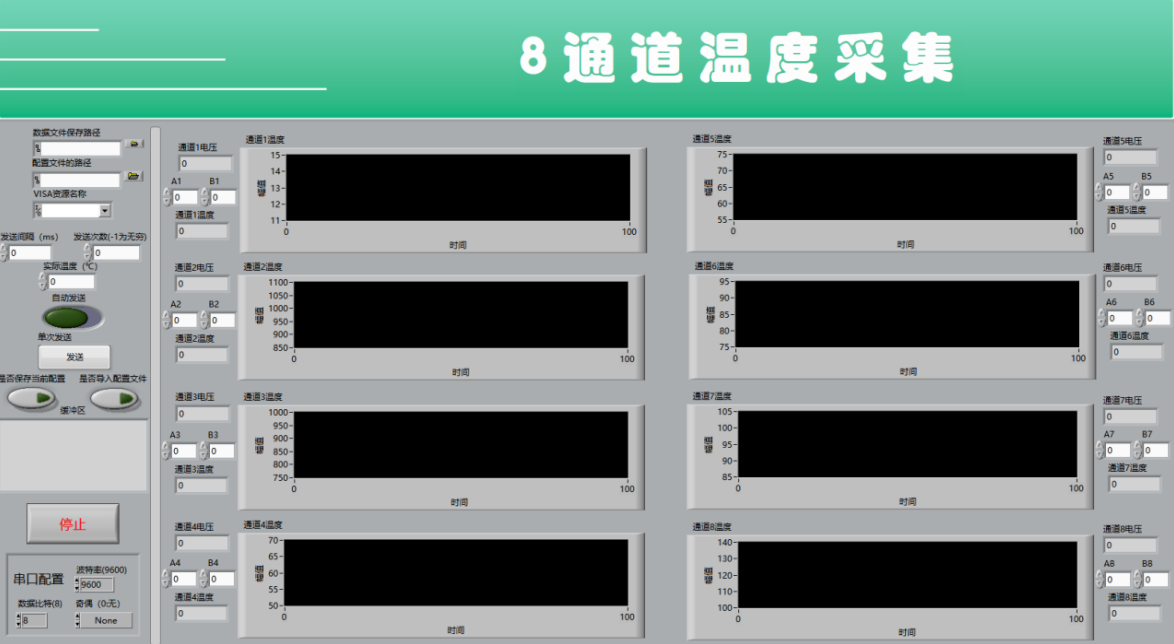
\includegraphics[width=14cm]{fig/3-fig/温度采集上位机前面板.jpg}
    \caption{温度测量上位机前面板}
    \label{fig:温度测量上位机前面板}
\end{figure}

图\ref{fig:温度测量上位机前面板}右边可见8个通道当前的标定系数,以及温度的实时测量值,而过去一段时间内的温度测量值的变化趋势则会以曲线的形式显示,用户界面的左列则为用户控制区,可进行以下参数的设定:
\begin{enumerate}
    \item 数据文件保存路径:选择测量数据保存的文件夹,程序会自动在该文件夹产生csv文件,文件的命名格式为年月日,如20210129。
    \item 配置文件的路径:选择配置文件路径,上位机软件会根据该配置文件里的系数计算温度值,配置文件通常由程序自带标定拟合功能产生。
    \item 自动发送:自动采集模式与手动采集模式的选择开关,若为自动采集模式,则根据“发送间隔”和“发送次数”两个参数,每隔一段时间进行一次采集,达到采集次数之后程序停止;若为手动采集模式则每次单机“发送”按钮后进行一次采集。
    \item 发送间隔:自动发送模式下,每次发送采集命令之间的时间间隔。
    \item 发送次数:自动发送模式下,发送采集命令的总次数(即采集次数),-1为无穷次。
    \item 实际温度:用于记录当前的实际温度,会在产生的csv文件中有记录,该项主要用于系统标定时。
    \item 串口配置:设置串口的波特率、数据比特位宽以及奇偶校验位。
  \end{enumerate}

\subsection{标定过程及结果}
基于PT100电阻的多通道温度测量系统标定过程如图\ref{fig:标定示意图}所示,在中空的热承中灌导热系数较好的油,并在热承下放置半导体制冷片,半导体制冷片下方放置散热片,两者接触面均匀涂抹导热硅脂,其余位置用黑色保温棉包裹,将待标定的PT100温度传感器捆绑在一起,减少温度不均性带来的误差。使用TCM-X107数字温控模块控制半导体制冷片,并在\(16^{\circ}C \sim 26^{\circ}C\)范围内取定几个温度点作为标定点,采用高精度温度传感器T520进行标定,每个标定待温度稳定之后,以\(0.5Hz\)的采样频率,采集一百个数据,去除最大值和最小值之后,以这98个点的平均值作为待标定数据。
  \begin{figure}[htb]
    \centering
    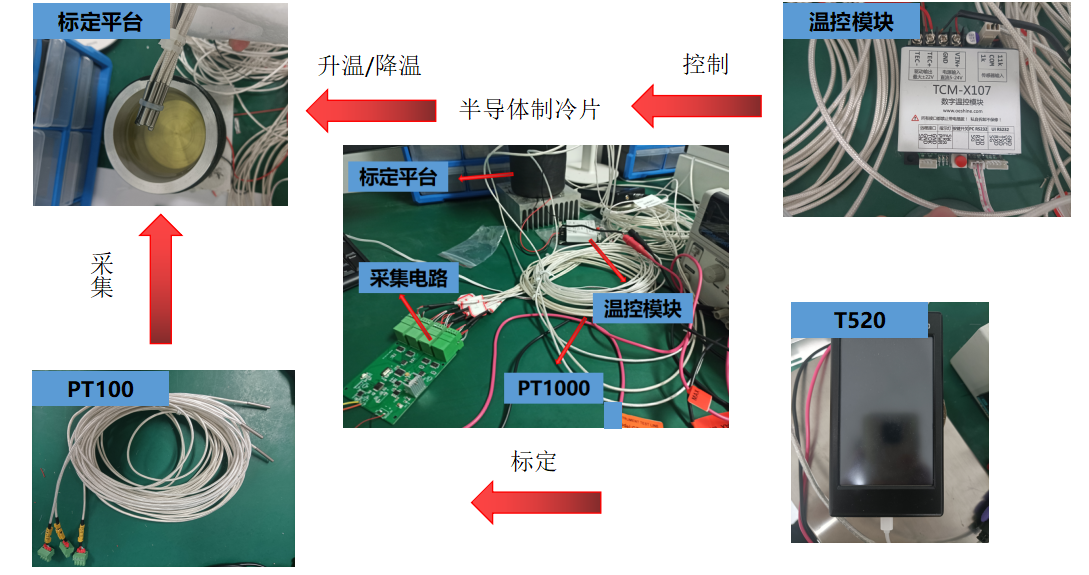
\includegraphics[width=12cm]{fig/3-fig/温度测量系统标定示意图.jpg}
    \caption{标定示意图}
    \label{fig:标定示意图}
\end{figure}

标定程序界面如图\ref{fig:标定程序用户界面}所示,红色的点为8个通道采集到的离散的温度数据,蓝色曲线为标定程序输出的拟合曲线,程序会自动根据标定结果生成.ini配置文件,供测量系统上位机使用。
\begin{figure}[htb]
    \centering
    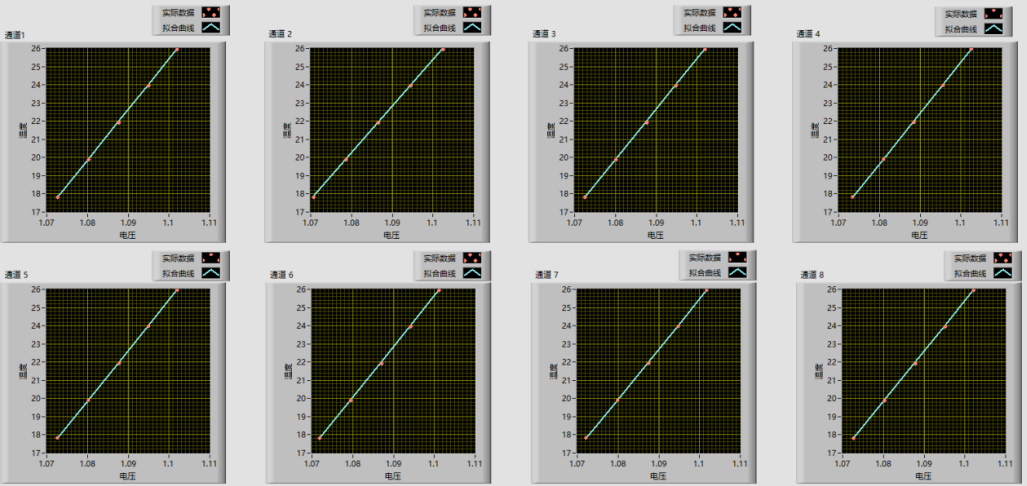
\includegraphics[width=12cm]{fig/3-fig/标定程序前面板.jpg}
    \caption{标定程序用户界面}
    \label{fig:标定程序用户界面}
\end{figure}

部分标定结果如表\ref{tab:标定误差值}所示,在所有标定结果中最大误差为$0.038^{\circ}C$,部分点误差大于$0.01^{\circ}C$,绝大部分点误差小于$0.01^{\circ}C$,并且8个通道的拟合优度$R^2$值都大于0.9999。
\begin{table}[H]
    \centering
    \caption{标定误差值}
    \label{tab:标定误差值}
    \resizebox{\textwidth}{14mm}{
    \begin{tabular}{ccccccccc}
        \hline
                      &   通道1/$^{ \circ}C$ & 通道2/$^{ \circ}C$ & 通道3/$^{ \circ}C$ & 通道4/$^{ \circ}C$ & 通道5/$^{ \circ}C$ & 通道6/$^{ \circ}C$ & 通道7/$^{ \circ}C$ & 通道8/$^{ \circ}C$ \\ \hline
    17.804$^{\circ}C$ & -0.0037 & 0.0037 & 0.0176 & 0.0072  & -0.0112 & 0.0101  & -0.0192 & -0.0279  \\ \hline
    19.879$^{\circ}C$ & 0.0008  & 0.0142 & 0.0209 & 0.0075  & 0.0030  & 0.0161  & -0.0052 & -0.0127  \\ \hline
    21.944$^{\circ}C$ & -0.0042 & 0.0022 & 0.0051 & -0.0037 & 0.0008  & -0.0015 & -0.0029 & -0.0030  \\ \hline
    24.047$^{\circ}C$ & 0.0008  & 0.0049 & 0.0123 & 0.0068  & 0.0033  & 0.0039  & -0.0074 & -0.0169  \\ \hline
    26.107$^{\circ}C$ & 0.0071  & 0.0017 & 0.0173 & 0.0116  & 0.0016  & 0.0078  & -0.0108 & -0.0162  \\ \hline
    \end{tabular}}
  \end{table}
\section{气压测量系统}
气压测量系统采用美国GE Druck公司PACE1000传感器,如图\ref{fig:PACE1000气压传感器}所示,精度为4pa,能够支持最小值/最大值/平均值显示,长期稳定性高达0.01\%$Rdg$每年,带有可选择的图形显示以及数据存储功能\cite{PACE1000}。
\begin{figure}[htb]
    \centering
    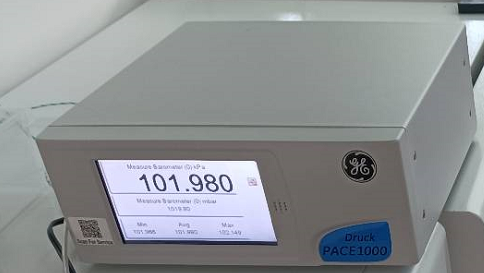
\includegraphics[width=8cm]{fig/3-fig/PACE1000气压传感器.jpg}
    \caption{PACE1000气压传感器}
    \label{fig:PACE1000气压传感器}
\end{figure}

\section{补偿系统总体方案}
补偿系统总体包括一套单轴双频激光干涉仪测量系统、隔震光学平台、温度测量模块和压力传感器四个部分,单轴双频激光干涉仪测量系统所用的的激光器为Agilent公司的5517A双频激光器,其名义波长为632.991354$nm$,1小时内的激光波长稳定性为0.002$ppm$,在90$mm$光程下,激光器自带的波长误差约为0.18$nm$,实物图如图\ref{fig:激光器实物图}所示。
\begin{figure}[htb]
    \centering
    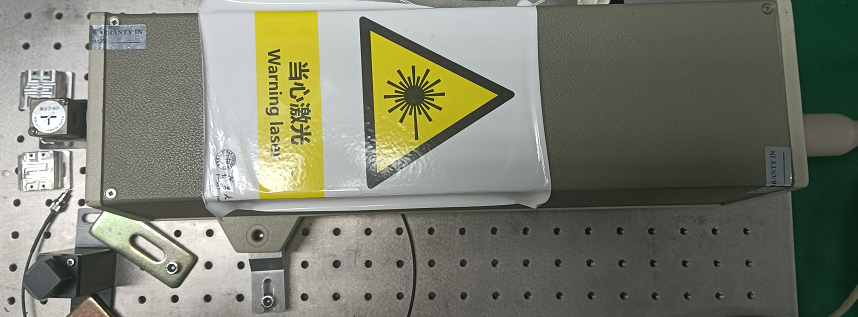
\includegraphics[width=10cm]{fig/3-fig/激光器实物图.png}
    \caption{激光器实物图}
    \label{fig:激光器实物图}
\end{figure}

干涉仪的光学细分为4,为了减小温度对材料热胀冷缩的影响,本文工作所用的干涉仪采用光学元件直接粘接制成,并无任何的金属外壳等,并且将底座粘接在微晶玻璃上,如图\ref{fig:干涉仪实物图}所示,微晶玻璃为德国肖特SCHOTT公司Class0级的微晶玻璃,其热膨胀系数小于$2\times 10^{-8}$,对于本文采用的测量臂长度为60$mm$和90$mm$的两套单周双频激光干涉仪,当温度变化$1^{ \circ}C$时,由于材料热胀冷缩引入的误差不会超过1.8$nm$,相对于环境误差而言,这是可以忽略不计的。
\begin{figure}[htb]
    \centering
    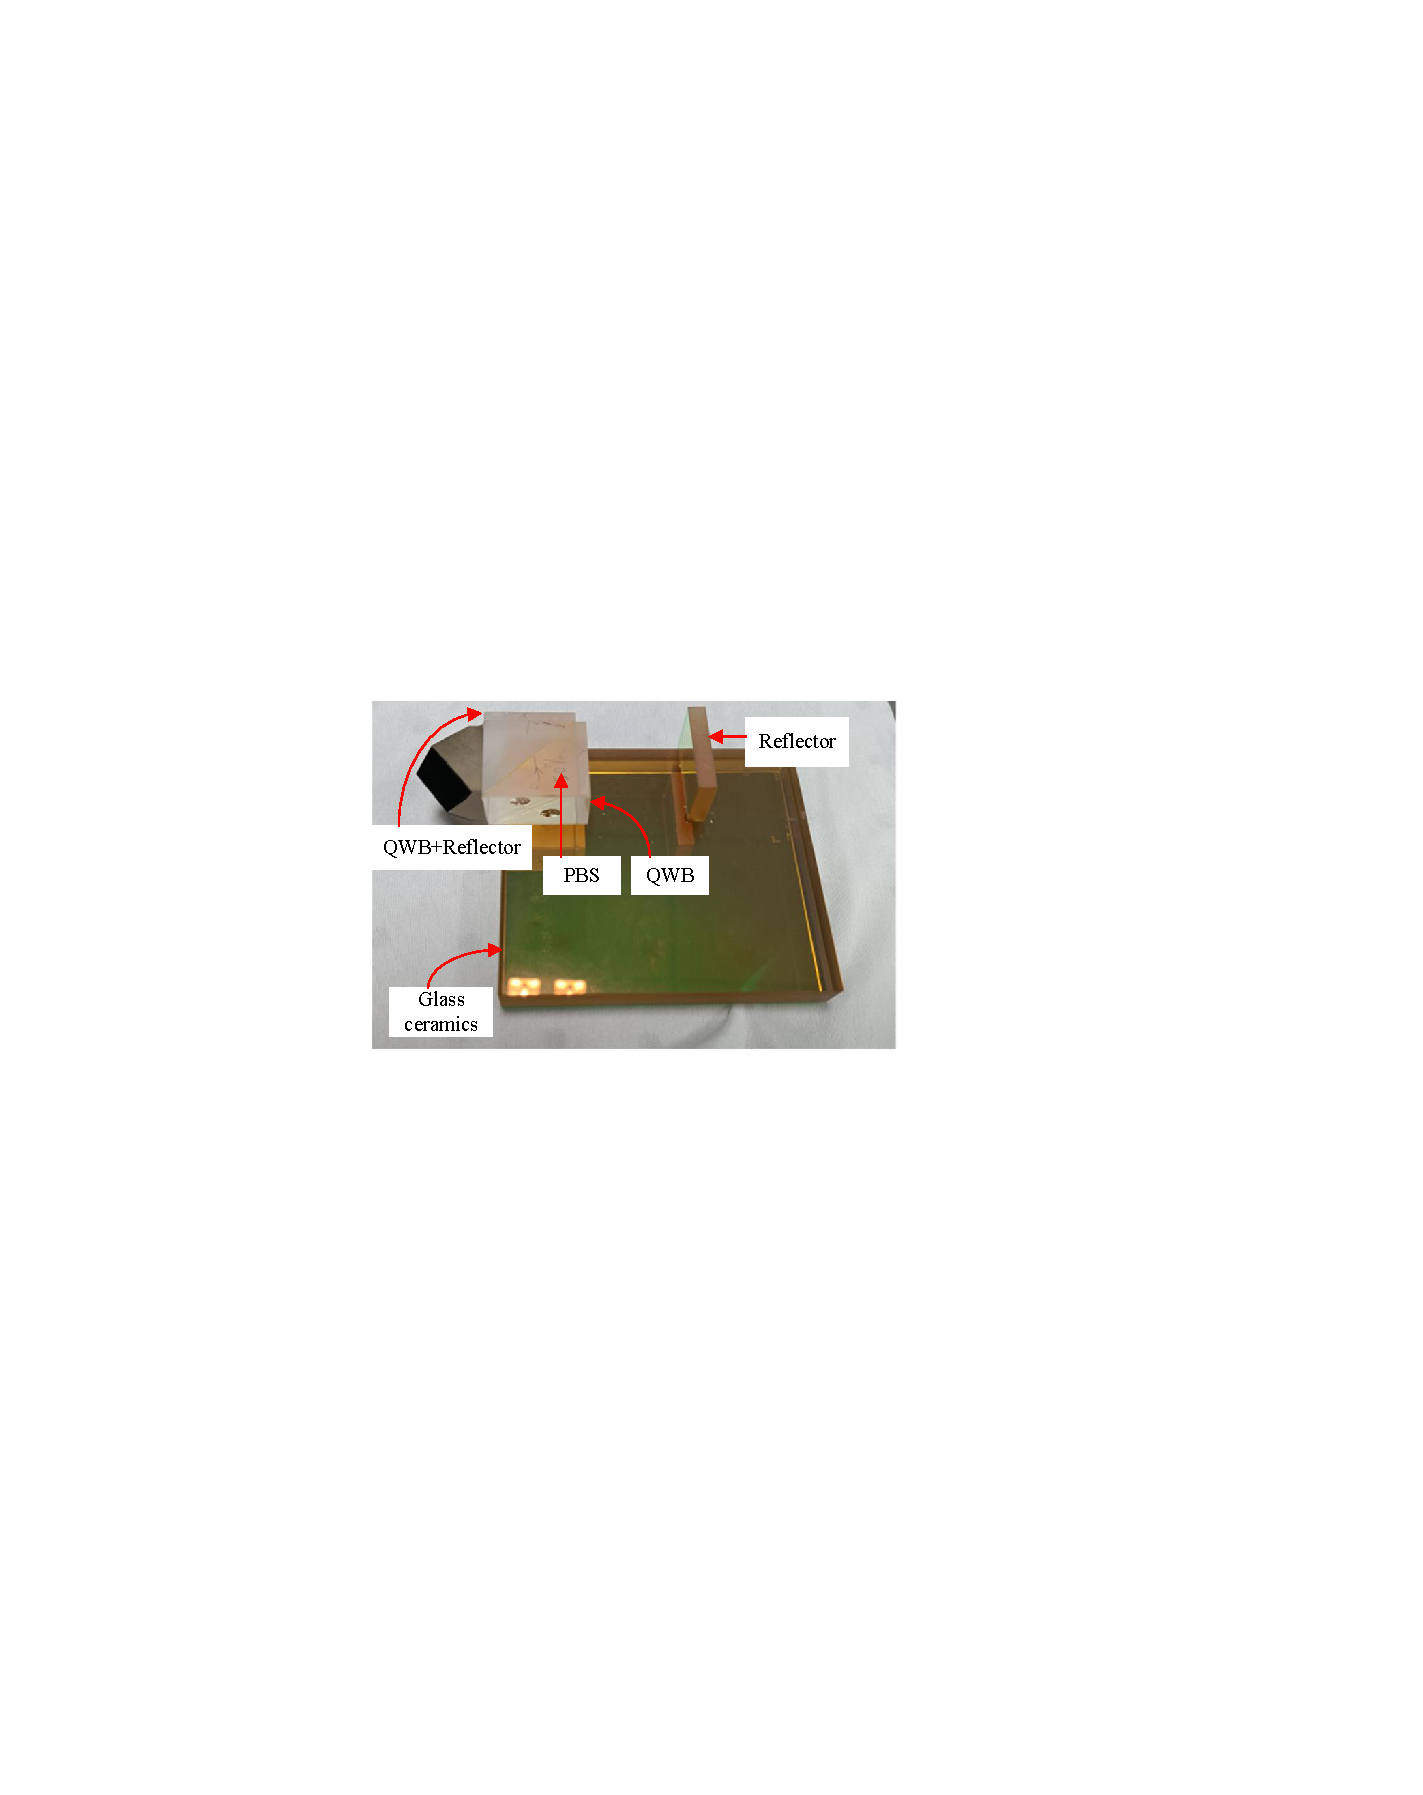
\includegraphics[width=8cm]{fig/3-fig/干涉仪实物图.pdf}
    \caption{干涉仪实物图}
    \label{fig:干涉仪实物图}
\end{figure}

系统中使用的信号采集卡为上海拍频光电科技有限公司的ELIB0306A三轴外差信号解调器,如图\ref{fig:信号采集卡实物图}所示,电子细分为32,信号采样率为$10MHz$,最多支持3个通道同时采样\cite{信号处理卡}。根据式\eqref{eq:分辨率与细分的关系}可知,该单轴双频激光干涉仪系统的分辨率约为4.9$nm$,这也再次说明了,上述的激光器自带的波长误差以及微晶玻璃热胀冷缩的影响可以忽略不计。
\begin{figure}[htb]
    \centering
    \includegraphics[width=8cm]{fig/3-fig/信号采集卡实物图.jpg}
    \caption{信号采集卡实物图}
    \label{fig:信号采集卡实物图}
\end{figure}

\section{实验方案及其改进}
在本文所述工作中,为了能够更精准地测量到干涉仪的环境误差,在实验方案上进行了多次改进:
\begin{enumerate}
    \item 实验设备方面:将干涉仪从常见的带有金属外壳的干涉仪改变为将各光学器件直接粘接制成的干涉仪以减少热胀冷缩带来的误差。
    \item 实验变量方面:从仅测量温度变为温度气压同时测量,虽然温度是影响干涉仪环境误差的最重要因素,但是仅仅对温度变量进行补偿无法满足精度要求,所以增加气压变量的补偿。
    \item 实验环境方面:从不采取任何隔震措施变为使用带有气浮隔震功能的光学平台,以减小震动带来的误差干扰;从有热源控制温度测量环境误差变为完全使用环境温度的自然变换来测量环境误差,以消除热源带来的误差干扰。
    \item 实验方法方面:从单一实验变为对比实验,由式\eqref{eq:环境误差公式}可以看出,干涉仪的环境误差是跟测量臂长度成正比的,所以衡量干涉仪环境误差补偿是否精准的方式即为判断不同测量臂长度下补偿后残差是否一致,一致即为精准补偿所以设立了60$nm$和90$nm$两种测量臂长度的实验组。
  \end{enumerate}
\subsection{实验设备改进}
传统的干涉仪如图\ref{fig:带金属外壳的干涉仪}所示,光学元器件粘贴在金属底座上,并且置有金属外壳。采用该种干涉仪的实验装置图如图\ref{fig:实验系统图-带外壳干涉仪}所示,进行零位测量得到的测量数据如图\ref{fig:带外壳干涉仪的实验数据}所示,可以看出在$7h$的测量时间里温度变化了约$0.6^\circ C$,但是干涉仪测出的位移却达到了$3000nm$,这个数量级的误差明显超出环境误差的范畴。并且由图\ref{fig:折射率-温度}可以看出,温度升高,空气折射率是降低的,带入\eqref{eq:环境误差公式}可知,由环境误差导致的干涉仪测量值应该是个负数,而实际测量值却是一个正数,所以大致可以断定是由于温度升高,导致干涉仪的金属底座以及被测物底座受热膨胀而导致出现正向位移误差值。所以后续采用如图\ref{fig:干涉仪实物图}所示的干涉仪,将PBS、反射镜、玻片等用光学胶直接粘接制成,并且干涉仪和被测物(反射镜)都直接粘在微晶玻璃上,以减小热胀冷缩带来的误差。
\begin{figure}[htb]
    \centering
    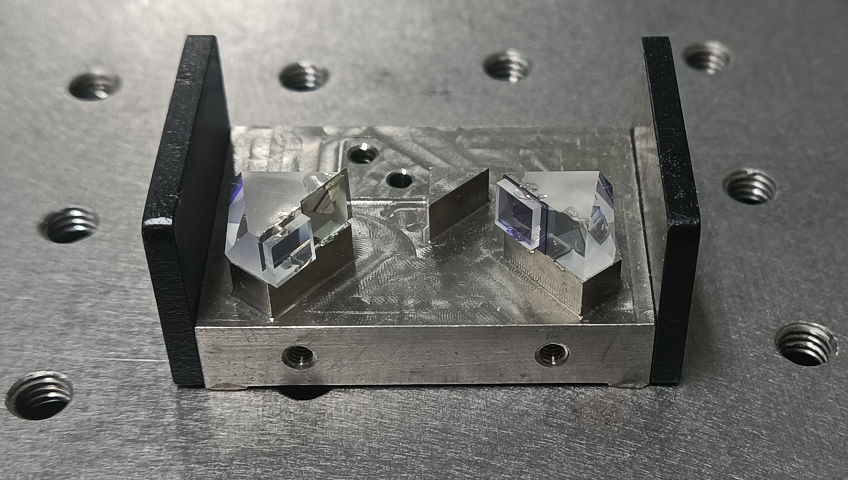
\includegraphics[width=6cm]{fig/3-fig/带金属外壳的干涉仪.png}
    \caption{带金属外壳的干涉仪}
    \label{fig:带金属外壳的干涉仪}
\end{figure}
\begin{figure}[htb]
    \centering
    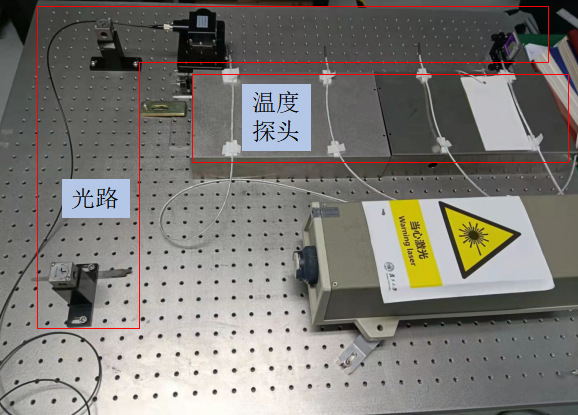
\includegraphics[width=8cm]{fig/3-fig/实验系统图-带外壳干涉仪.jpg}
    \caption{实验系统图-带外壳干涉仪}
    \label{fig:实验系统图-带外壳干涉仪}
\end{figure}
\begin{figure}[htb]
    \centering
    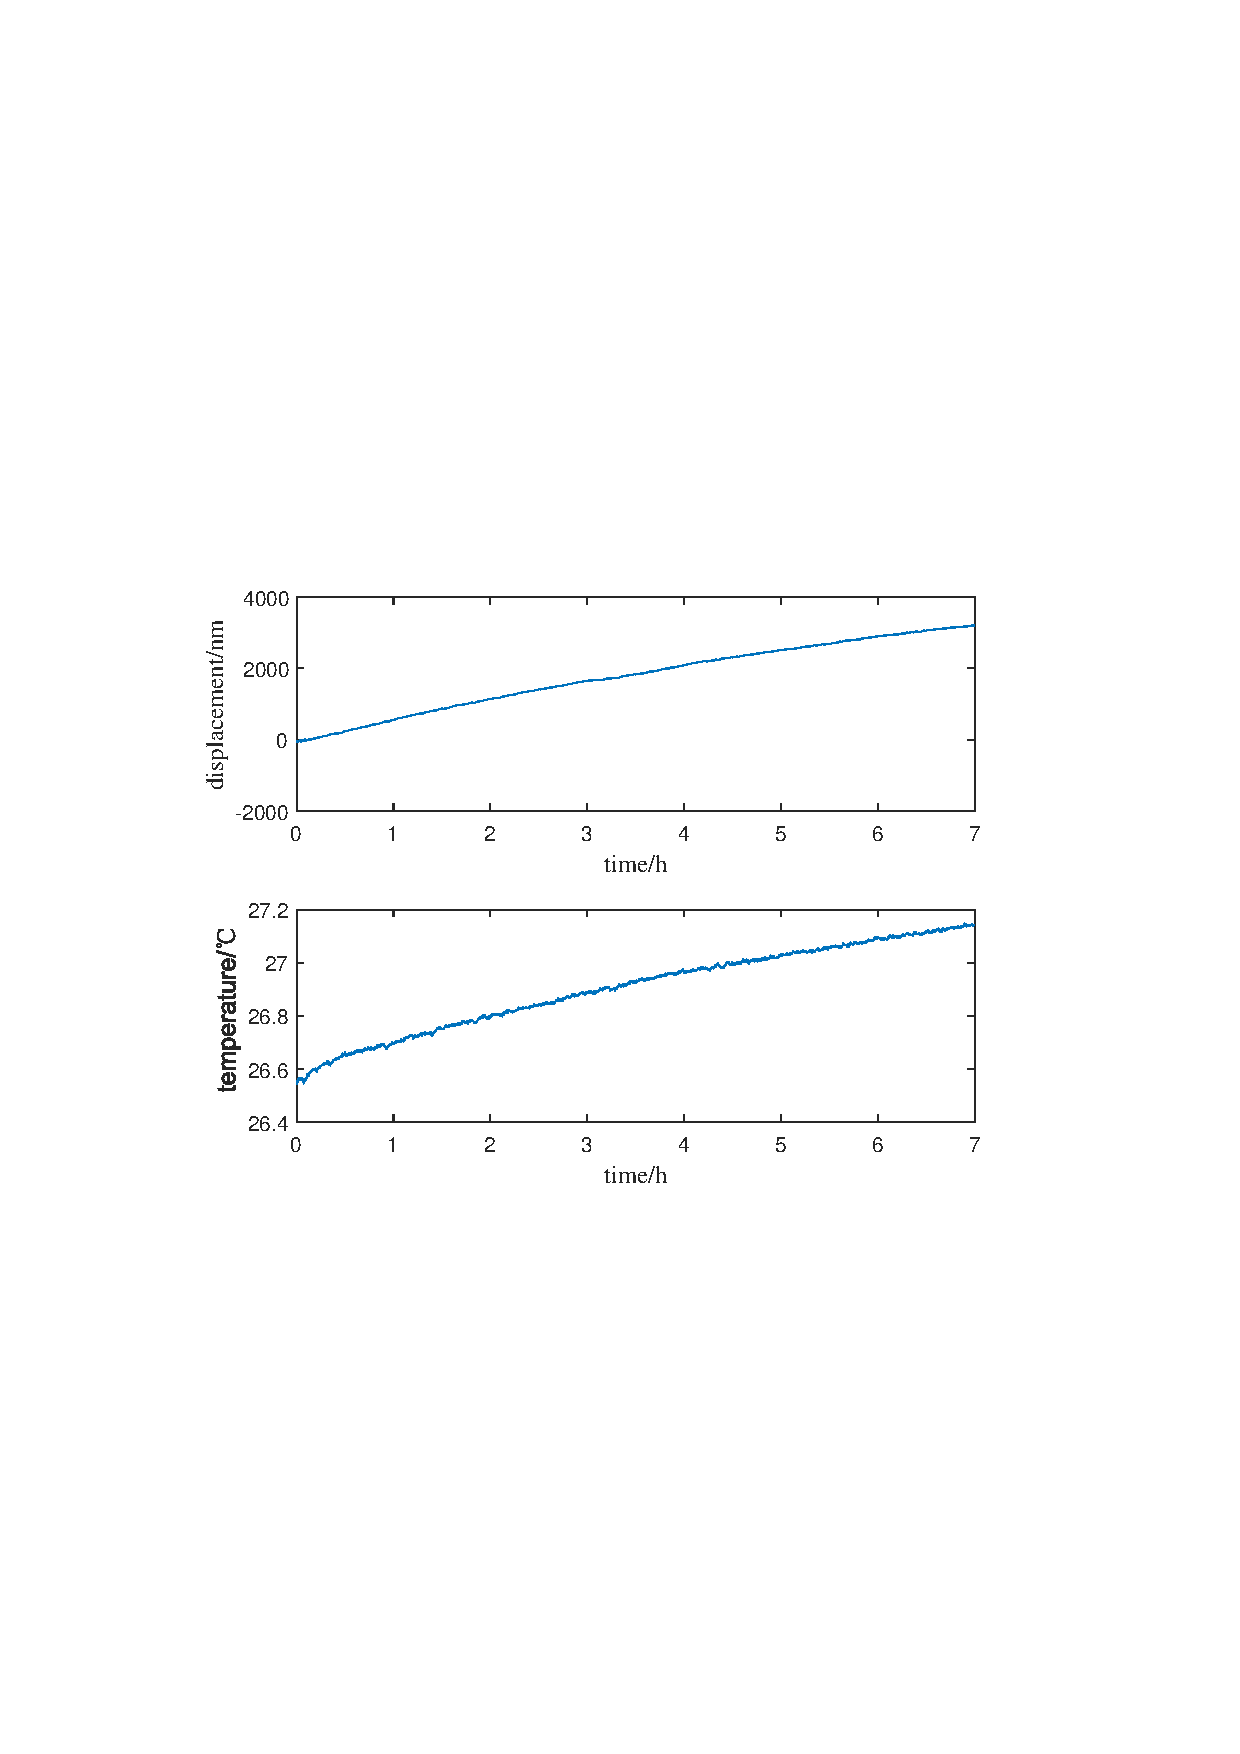
\includegraphics[width=12cm]{fig/3-fig/实验数据-带外壳的干涉仪.pdf}
    \caption{带外壳干涉仪的实验数据}
    \label{fig:带外壳干涉仪的实验数据}
\end{figure}

\subsection{实验变量改进}
将干涉仪和被测物体粘接在微晶玻璃后的实验装置如图\ref{fig:实验系统图-带微晶玻璃}所示,如前文所述,此时由于热胀冷缩带来的误差是可以忽略不计的。进行零位测量得到的测量数据如图\ref{fig:实验数据-带微晶玻璃}所示,从图中可以看出约$480nm$的环境误差,如果仅仅对温度这一单一变量进行误差补偿,残留误差仍有约$180nm$,虽然补偿了约$60\%$的误差,但是残余值仍不可以忽略,所以需要增加实验变量,即对气压也进行补偿。
\begin{figure}[htb]
  \centering
  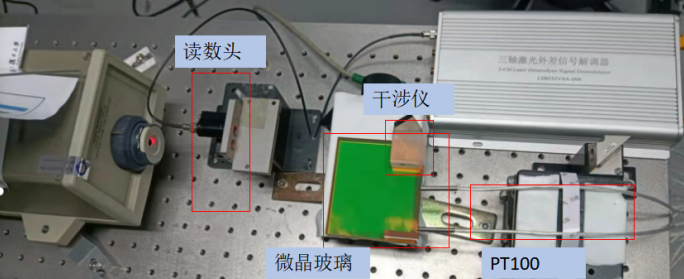
\includegraphics[width=12cm]{fig/3-fig/实验系统图-带微晶玻璃.jpg}
  \caption{实验系统图-带微晶玻璃}
  \label{fig:实验系统图-带微晶玻璃}
\end{figure}
\begin{figure}[htb]
  \centering
  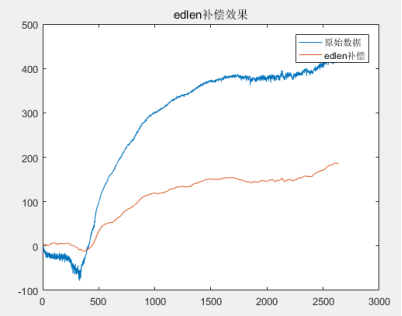
\includegraphics[width=7cm]{fig/3-fig/实验数据-带微晶玻璃.jpg}
  \caption{实验数据-带微晶玻璃}
  \label{fig:实验数据-带微晶玻璃}
\end{figure}

\subsection{实验环境改进}
带温控箱的实验装置图如图\ref{fig:带温控箱的实验装置图}所示,图\ref{fig:实验示意图-带温控箱}为示意图,图\ref{fig:实验系统图-带温控箱}为实物图。
\begin{figure}[htb]
    \centering
    \subfigure[实验示意图-带温控箱]{
      \begin{minipage}[b]{0.80\textwidth}
        \centering
        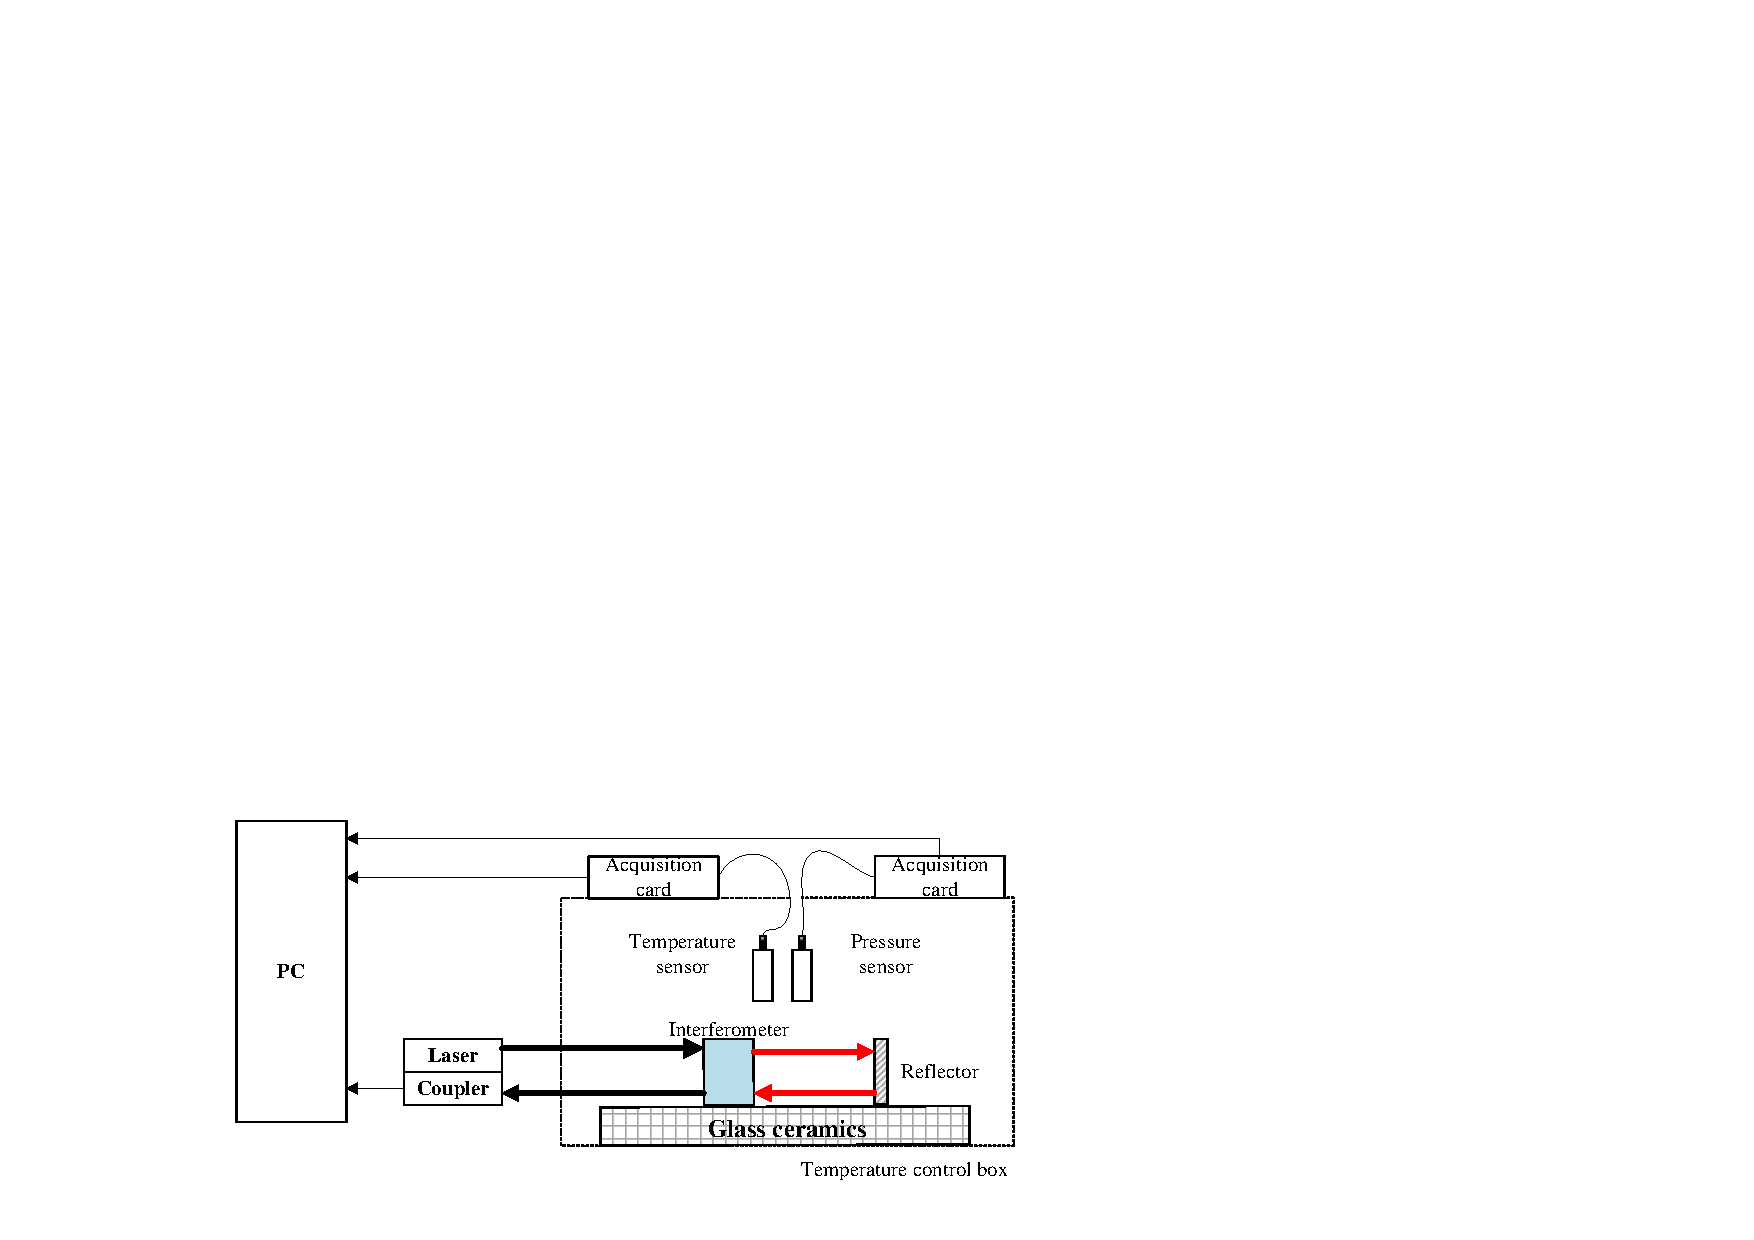
\includegraphics[width=10cm,height=5cm]{fig/3-fig/实验示意图-带温控箱.pdf}
      \end{minipage}
      \label{fig:实验示意图-带温控箱}
    }
    \subfigure[实验系统图-带温控箱]{
      \begin{minipage}[b]{0.80\textwidth}
        \centering
        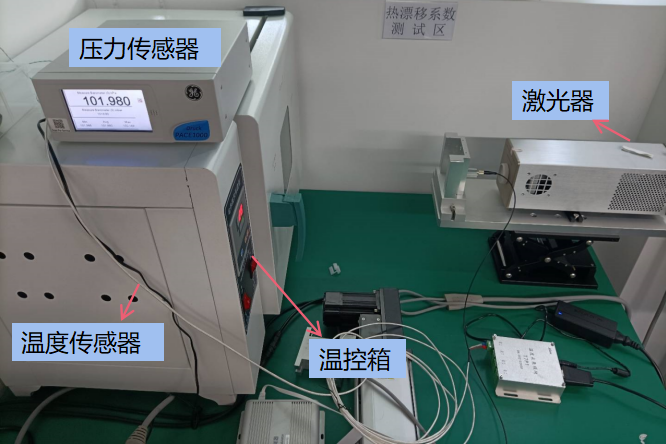
\includegraphics[width=9cm,height=6cm]{fig/3-fig/实验系统图-带温控箱.jpg}
      \end{minipage}
      \label{fig:实验系统图-带温控箱}
    }
    \caption{带温控箱的实验装置图}
    \label{fig:带温控箱的实验装置图}
  \end{figure}
实验数据如图\ref{fig:带温控箱的实验数据}所示,$5h$的测量时间内,温度变化约为$0.1^\circ C$,气压变化约为$0.25kPa$,排除了热胀冷缩的影响之后,位移的误差值降到了几十$nm$级别,属于环境误差的合理范畴但从图中可以明显看出,相较于平滑的压力曲线,温度曲线有着较多的毛刺,这也使得干涉仪系统的位移测量值也有着较多毛刺,这是由于温控箱工作导致的不均匀性引起的。所以后续实验采用测量环境温度的自然变化,并且增加气浮功能用于隔震。
\begin{figure}[htb]
    \centering
    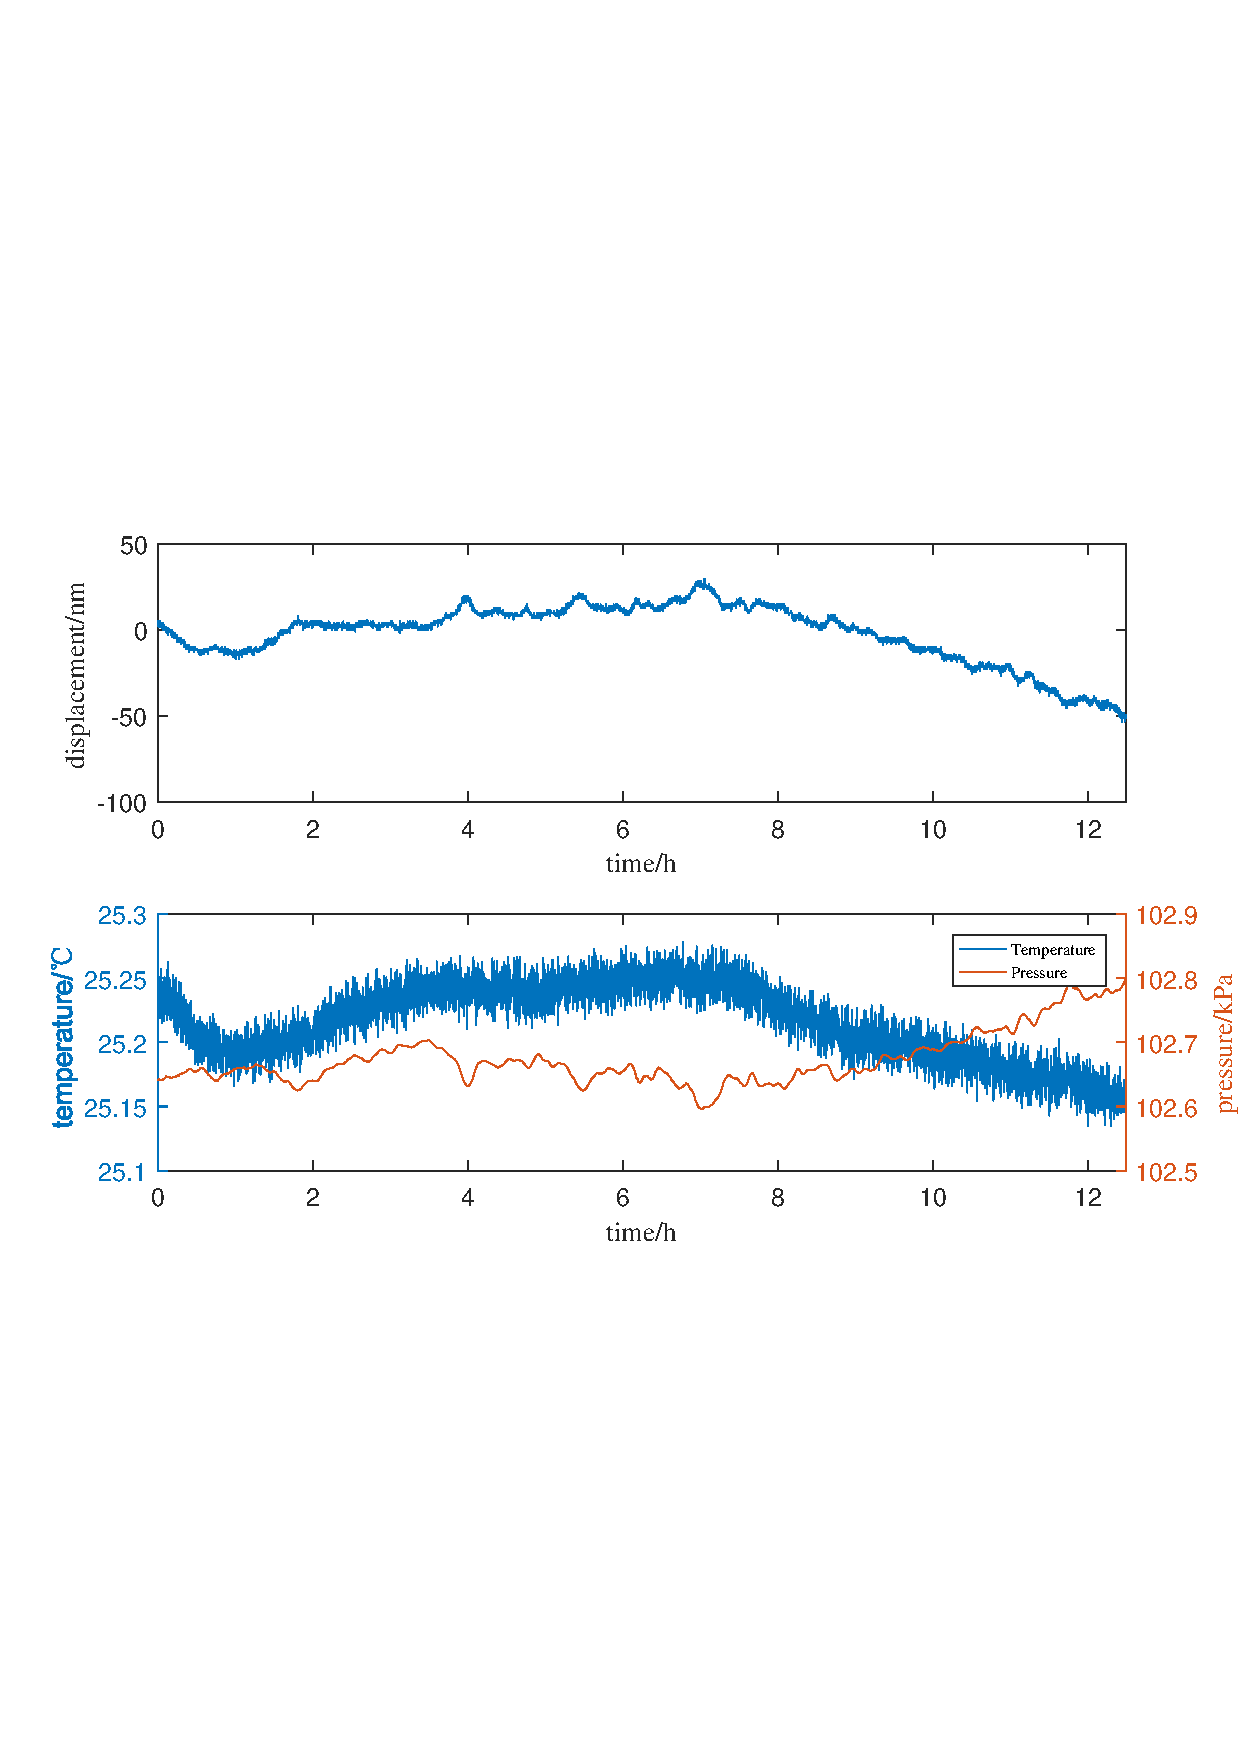
\includegraphics[width=12cm]{fig/3-fig/实验数据-温控箱.pdf}
    \caption{带温控箱的实验数据}
    \label{fig:带温控箱的实验数据}
\end{figure}

\subsection{最终实验方案}
最终实验方案如图\ref{fig:最终实验方案}所示,图\ref{fig:最终实验示意图}为示意图,图\ref{fig:最终实验系统图}为实物图。测量臂长度为$60nm$和$90nm$的两套干涉仪都是粘接在微晶玻璃上,并且放置在亚克力罩内,温度传感器探头和压力传感器探头也固体在亚克力罩内,激光器出射的激光经过$50\%$分光镜分成两束强度均匀的光后分别进入两套干涉仪系统,并且经两个光纤耦合器后接入采集板卡。所有光学器件都有卡座固定在光学平台,并且光学平台开启了气浮功能以减少震动的影响。
\begin{figure}[htb]
    \centering
    \subfigure[最终实验示意图]{
      \begin{minipage}[b]{0.90\textwidth}
        \centering
        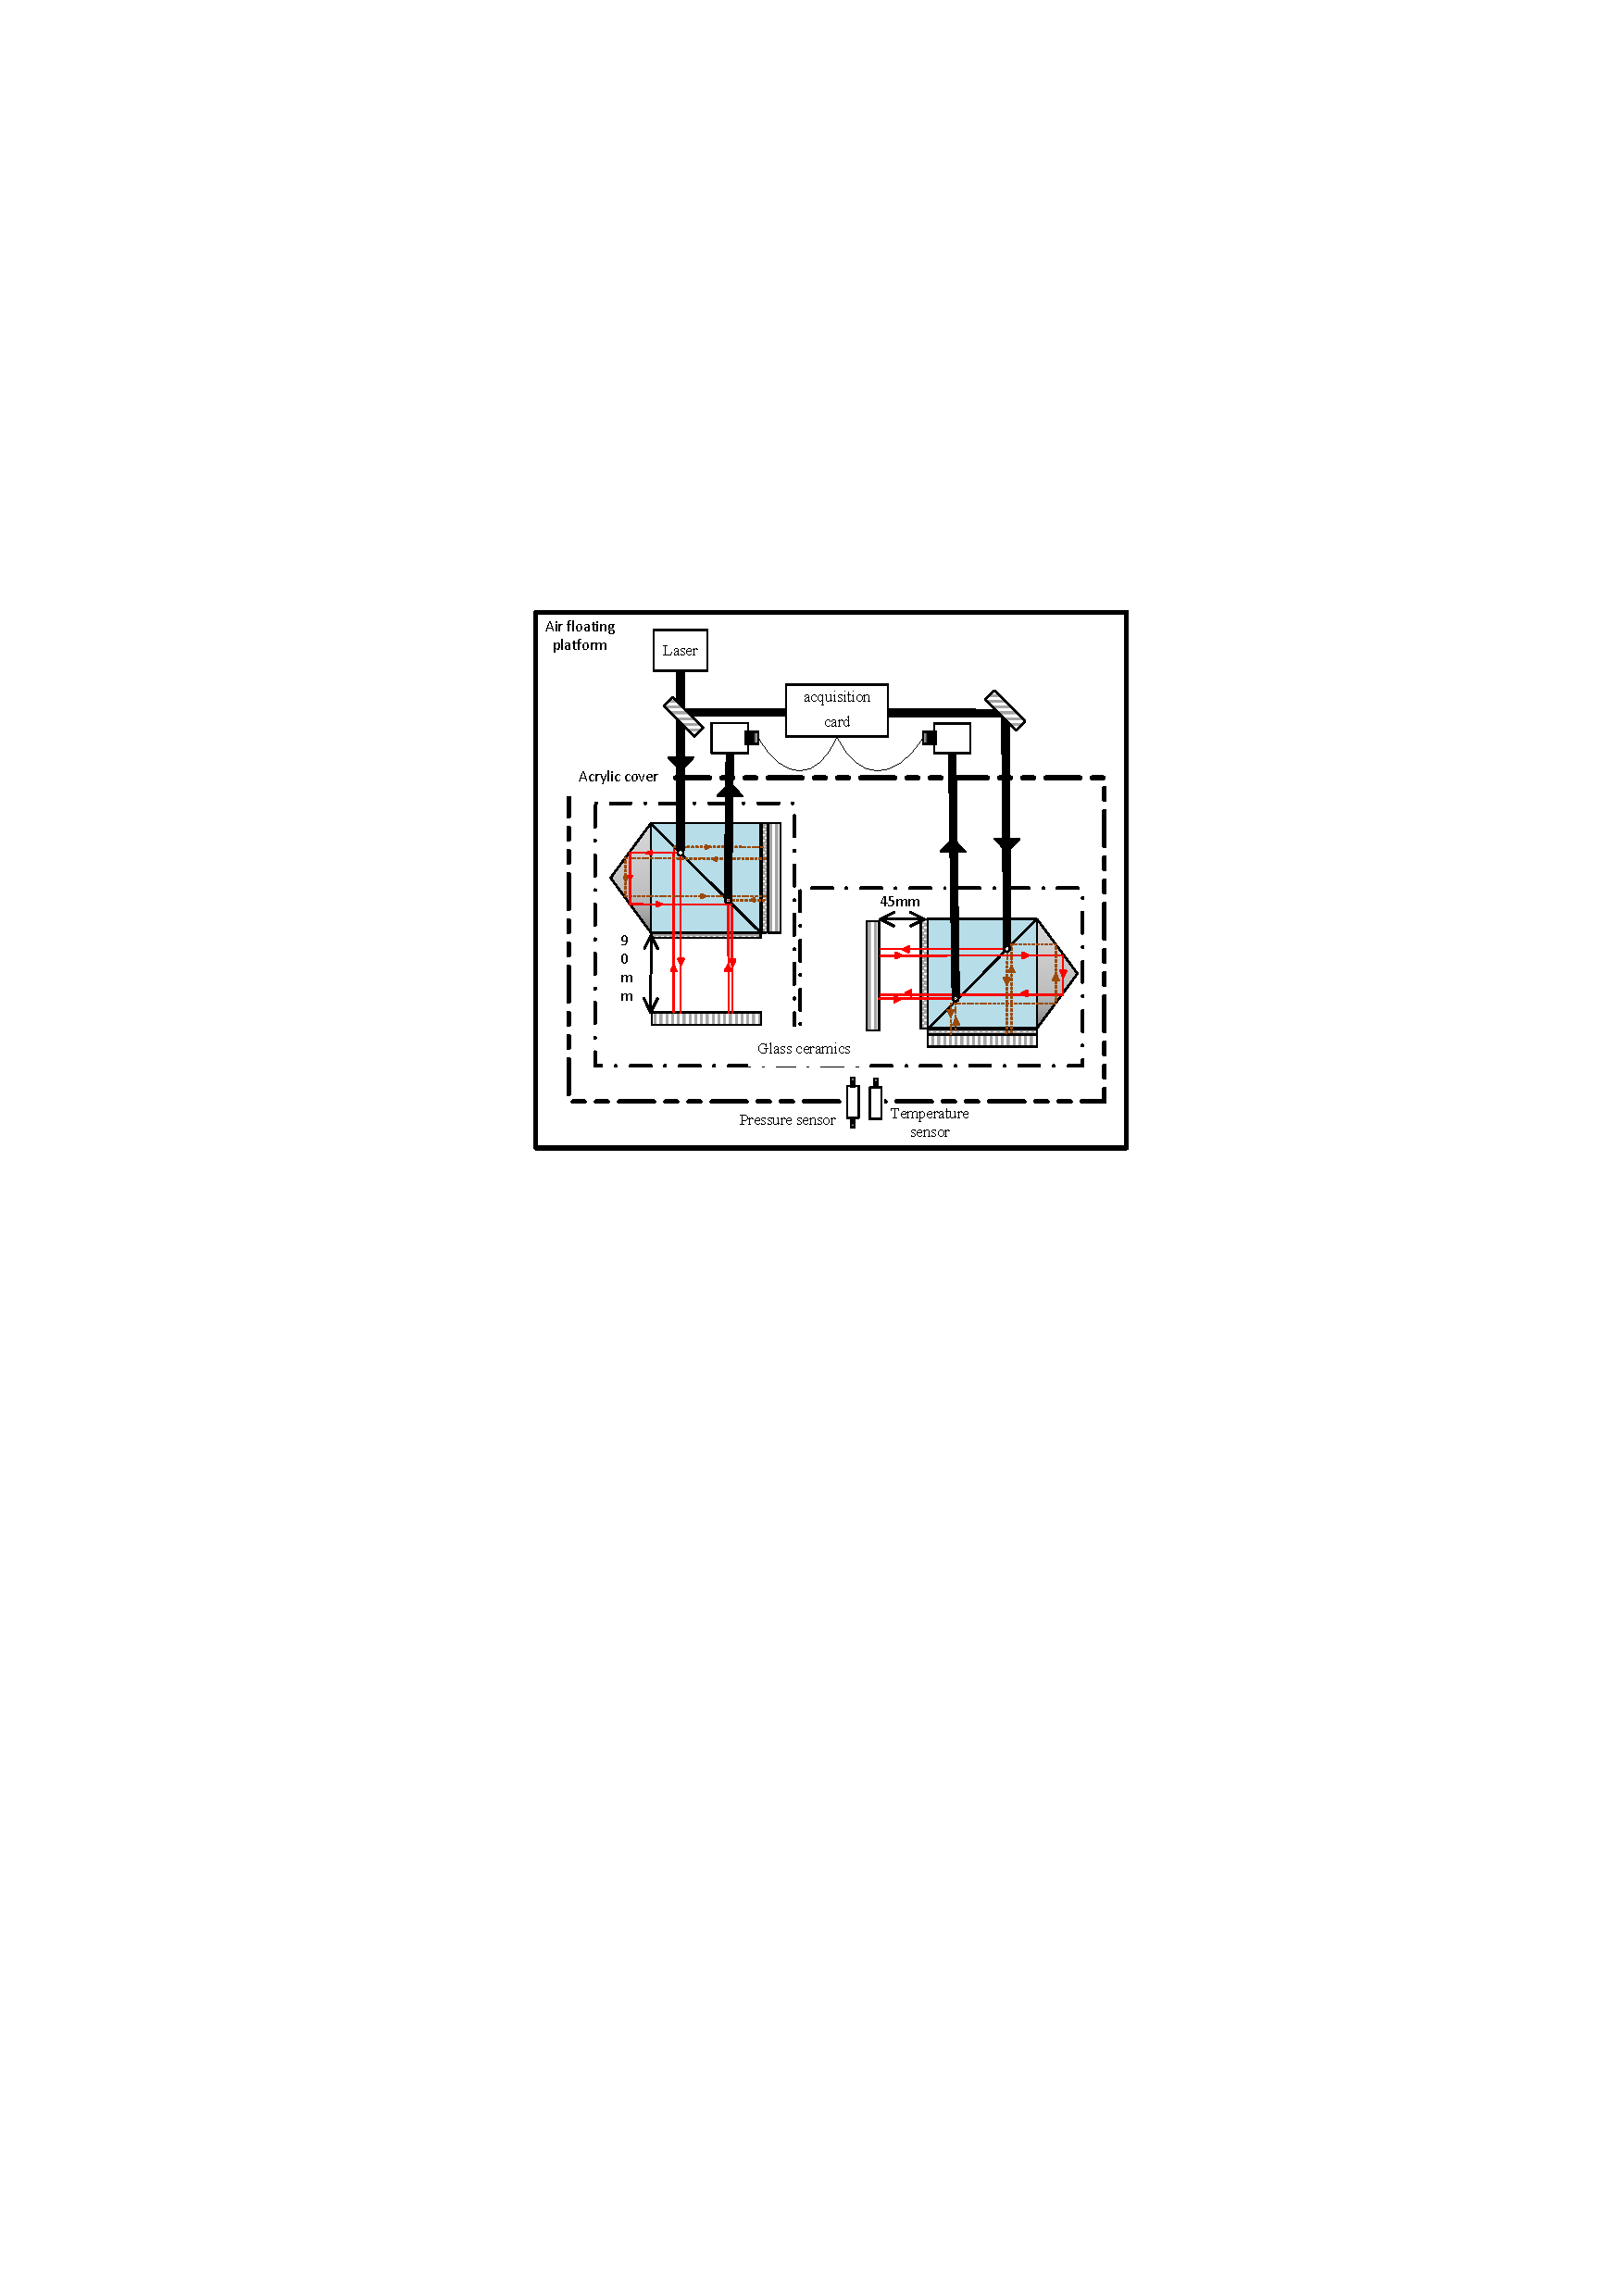
\includegraphics[width=9.5cm,height=6.5cm]{fig/3-fig/最终实验示意图.pdf}
      \end{minipage}
      \label{fig:最终实验示意图}
    }
    \subfigure[最终实验系统图]{
      \begin{minipage}[b]{0.90\textwidth}
        \centering
        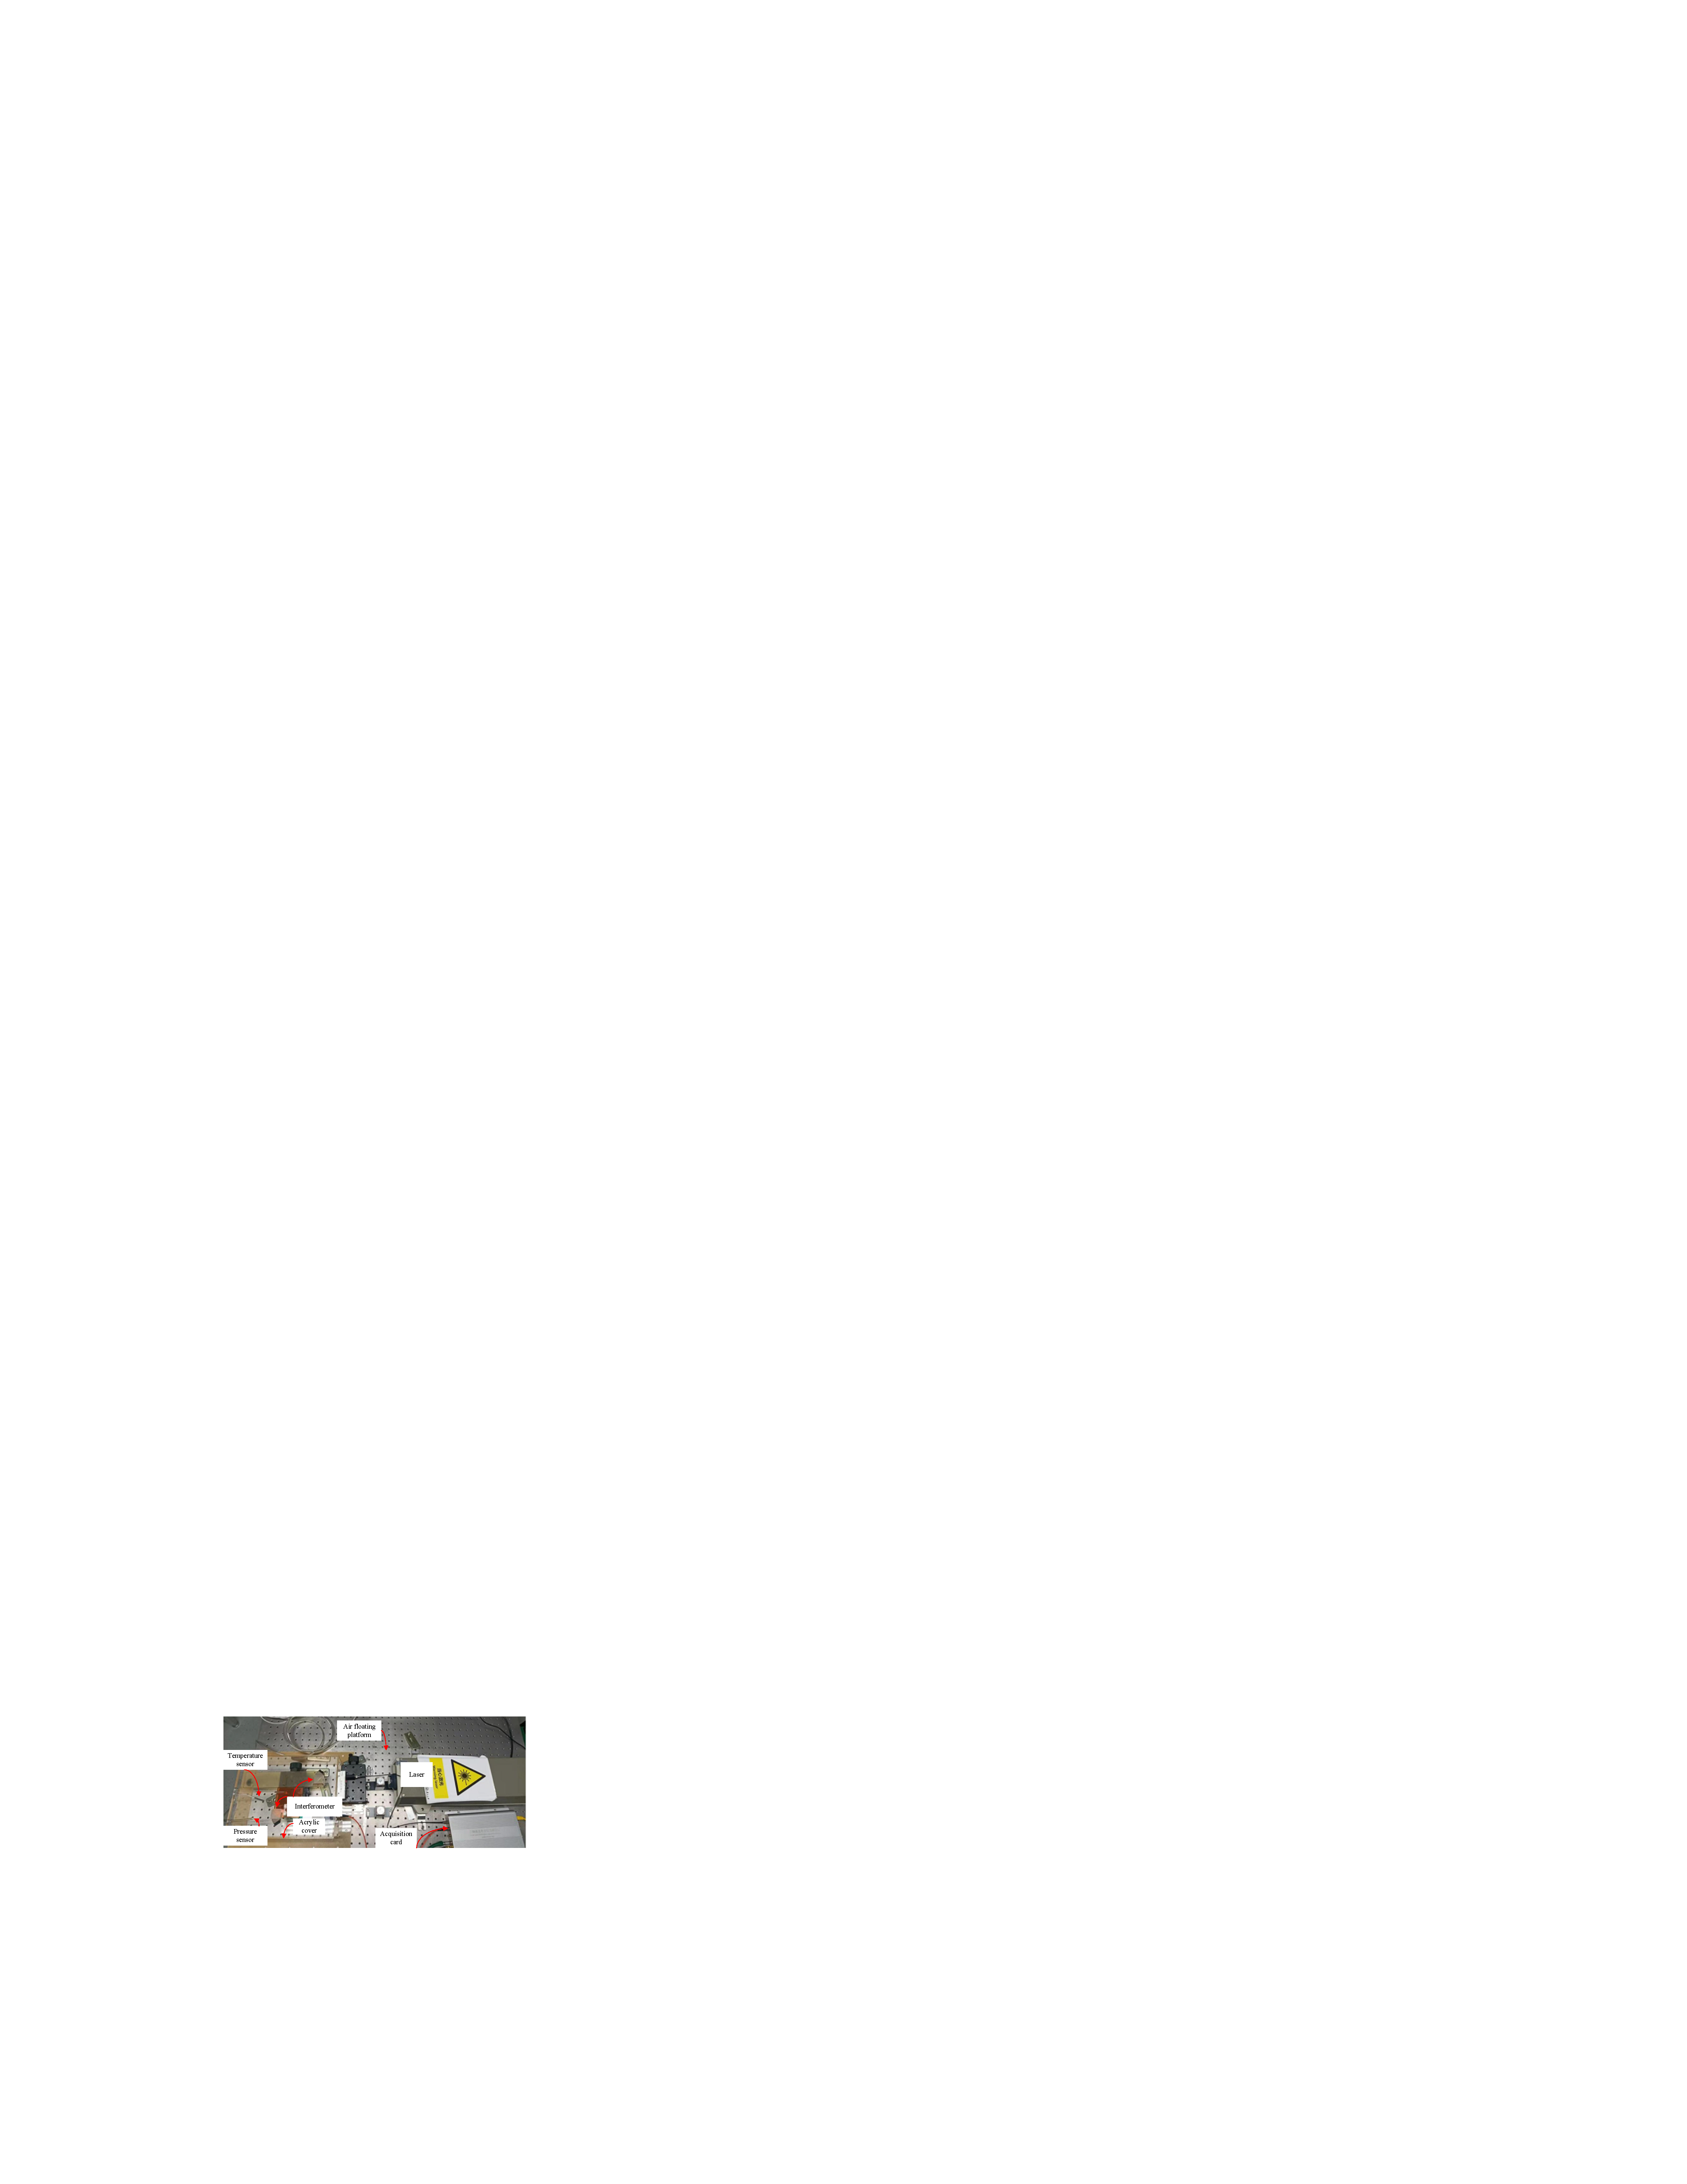
\includegraphics[width=12cm,height=5.5cm]{fig/3-fig/最终实验系统图.pdf}
      \end{minipage}
      \label{fig:最终实验系统图}
    }
    \caption{最终实验方案}
    \label{fig:最终实验方案}
  \end{figure}

\section{实验系统安装和调试}
上述实验系统的搭建时,主要按照以下基本流程进行:
\begin{enumerate}
    \item 将激光器放置在光学平台上,并进行固定,通电点亮激光器进行预热,待激光器尾部的指示灯亮起时说明预热结束,然后再次固定激光器。
    \item 将分光镜、干涉仪放置在光学平台上,并进行预固定。旋转激光器出口光阑,选择大光斑,随后调分光镜的的位置,确保光束从分光镜外壳通光孔的中心入射,并且没有出现消光现象,然后将激光器的光斑从大光斑调整为小光斑,调整干涉仪位置,确保干涉仪的反射镜与入射光束垂直;随后微调分光镜俯仰角以及干涉仪位置,使得干涉仪的测量光斑和参考光斑重合,并且光斑形状为圆形,然后固定分光镜和干涉仪位置。并将激光器的光斑调整为合适测量的光斑大小。
    \item 将亚克力罩罩在干涉仪上方,并且固定温度传感器和压力传感器,随后将亚克力罩也固定在光学平台上。
    \item 安装光纤耦合器,并将光纤接到采集板卡。
  \end{enumerate}
  \section{补偿性能测试与实验结果}
为了验证Edlen公式在波长不匹配、温度范围不匹配的情况下,仍然能对干涉仪的环境误差进行一定程度的补偿,但会使得精度所损失,进行了多次实验数据采集,部分结果如下文所述。所有实验的采样周期均为$2s$,所有测量均为零位测量,即理论位移应为0。并且从式\eqref{eq:环境误差公式}可以看出,干涉仪的环境误差是与测量臂长度成正比的,而其它误差(例如随机误差、非线性误差等)往往都与测量臂长度无关,由此可以得出判断干涉仪环境误差补偿是否精准的标志就是看补偿后的残差是否一致。

\subsection{短时测量}
如图\ref{fig:短时测量实验数据}所示,(a)图为测量臂长度为$45nm$的位移测量数据,(b)图为测量臂长度为$90nm$的位移测量数据,(c)图为对应的温度和气压数据,(a)、(b)、(c)三图的横轴均为时间,单位为h;(a)和(b)图中的竖轴为位移数据,单位为$nm$,其中带圆圈标注的蓝色曲线为原始的位移测量数据,带黄色方块标注的为使用原始Edlen公式补偿后的位移数据,(c)图的竖轴为温度和气压数据,单位为$^{\circ}C$和$kPa$,其中带圆圈标注的蓝色曲线为温度数据,红色曲线为气压数据。
\begin{figure}[htb]
    \centering
    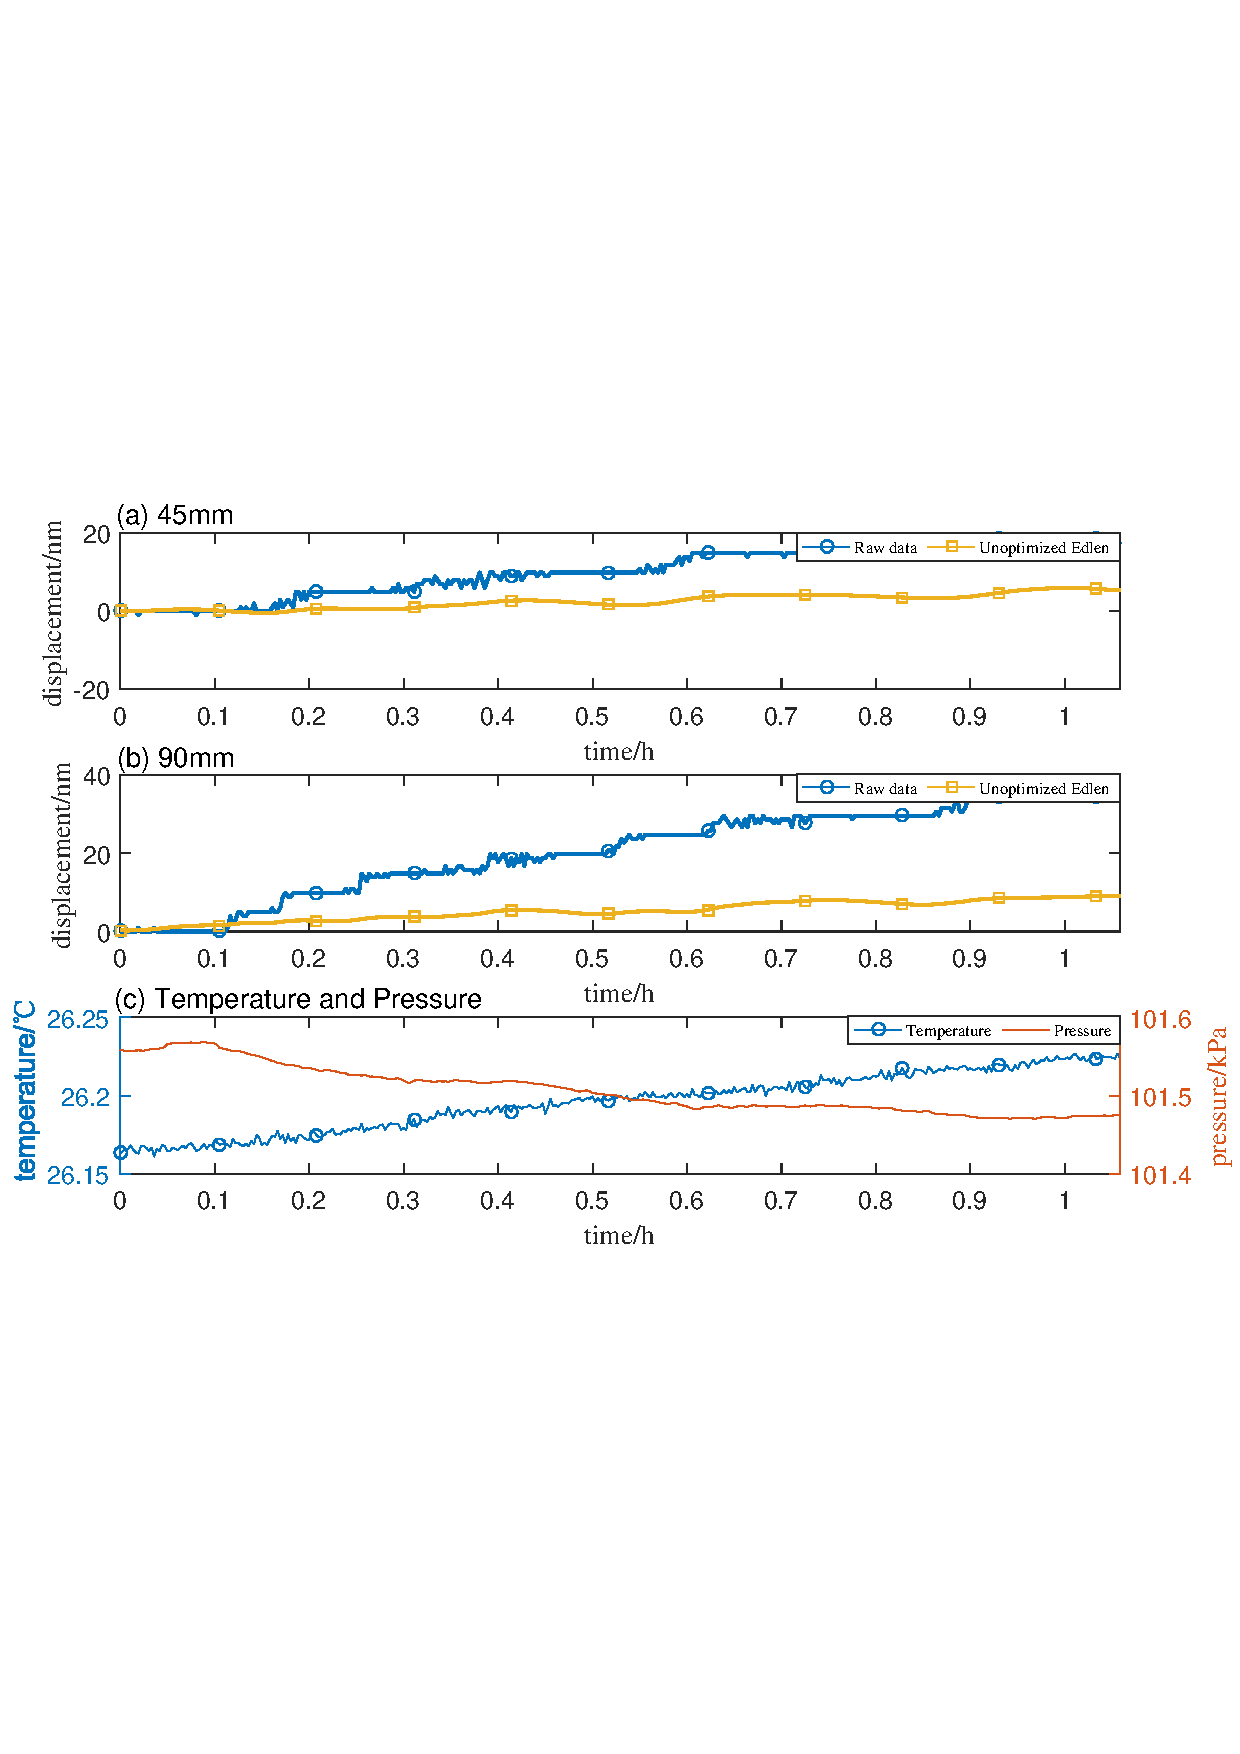
\includegraphics[width=14cm]{fig/3-fig/短时测量数据.pdf}
    \caption{短时测量实验数据}
    \label{fig:短时测量实验数据}
\end{figure}
从图中可以看出,测量时间约为$1h$,温度变化范围为$[26.16\,\,\,26.23]^{\circ}C$,气压变化范围为$[101.6\,\,\,101.5]kPa$,测量臂长度为$45nm$和$90nm$的两套干涉仪的原始位移数据的变化范围为$[0\,\,\,19.78]nm$和$[0\,\,\,34.62]nm$,在考虑可能含有随机误差等其他误差的情况下,可近似认为两者成两倍关系。并且对于零位测量而言,上述位移变化都可以认为是误差,对应的均方根误差分别为$11.8869nm$和$23.3770nm$,也符合式\eqref{eq:环境误差公式}中描述的关系,这也说明在测量过程中并未引入太多其他误差,导致干涉仪测量值变化的主要原因为环境因素。

经过Edlen公式补偿后的均方根误差为$3.1377nm$和$5.8401nm$,补偿效果约为$71\%$和$75\%$。可以看出使用Edlen公式进行干涉仪的环境误差补偿可以得到较好的补偿效果,但是经过Edlen公式补偿之后的残留均方根误差仍然近似成两倍关系,这说明由于温度不匹配、波长不匹配以及Edlen公式人为总结的局限性,使得Edlen公式在补偿后仍有部分环境误差残留。

\subsection{长时测量}
短时测量的时间$1h$左右,为了探究Edlen公式在长时间测量情况下的补偿效果,将测量时间增加到$7.5h$,得到的实验数据如图\ref{fig:长时测量实验数据}。
\begin{figure}[htb]
  \centering
  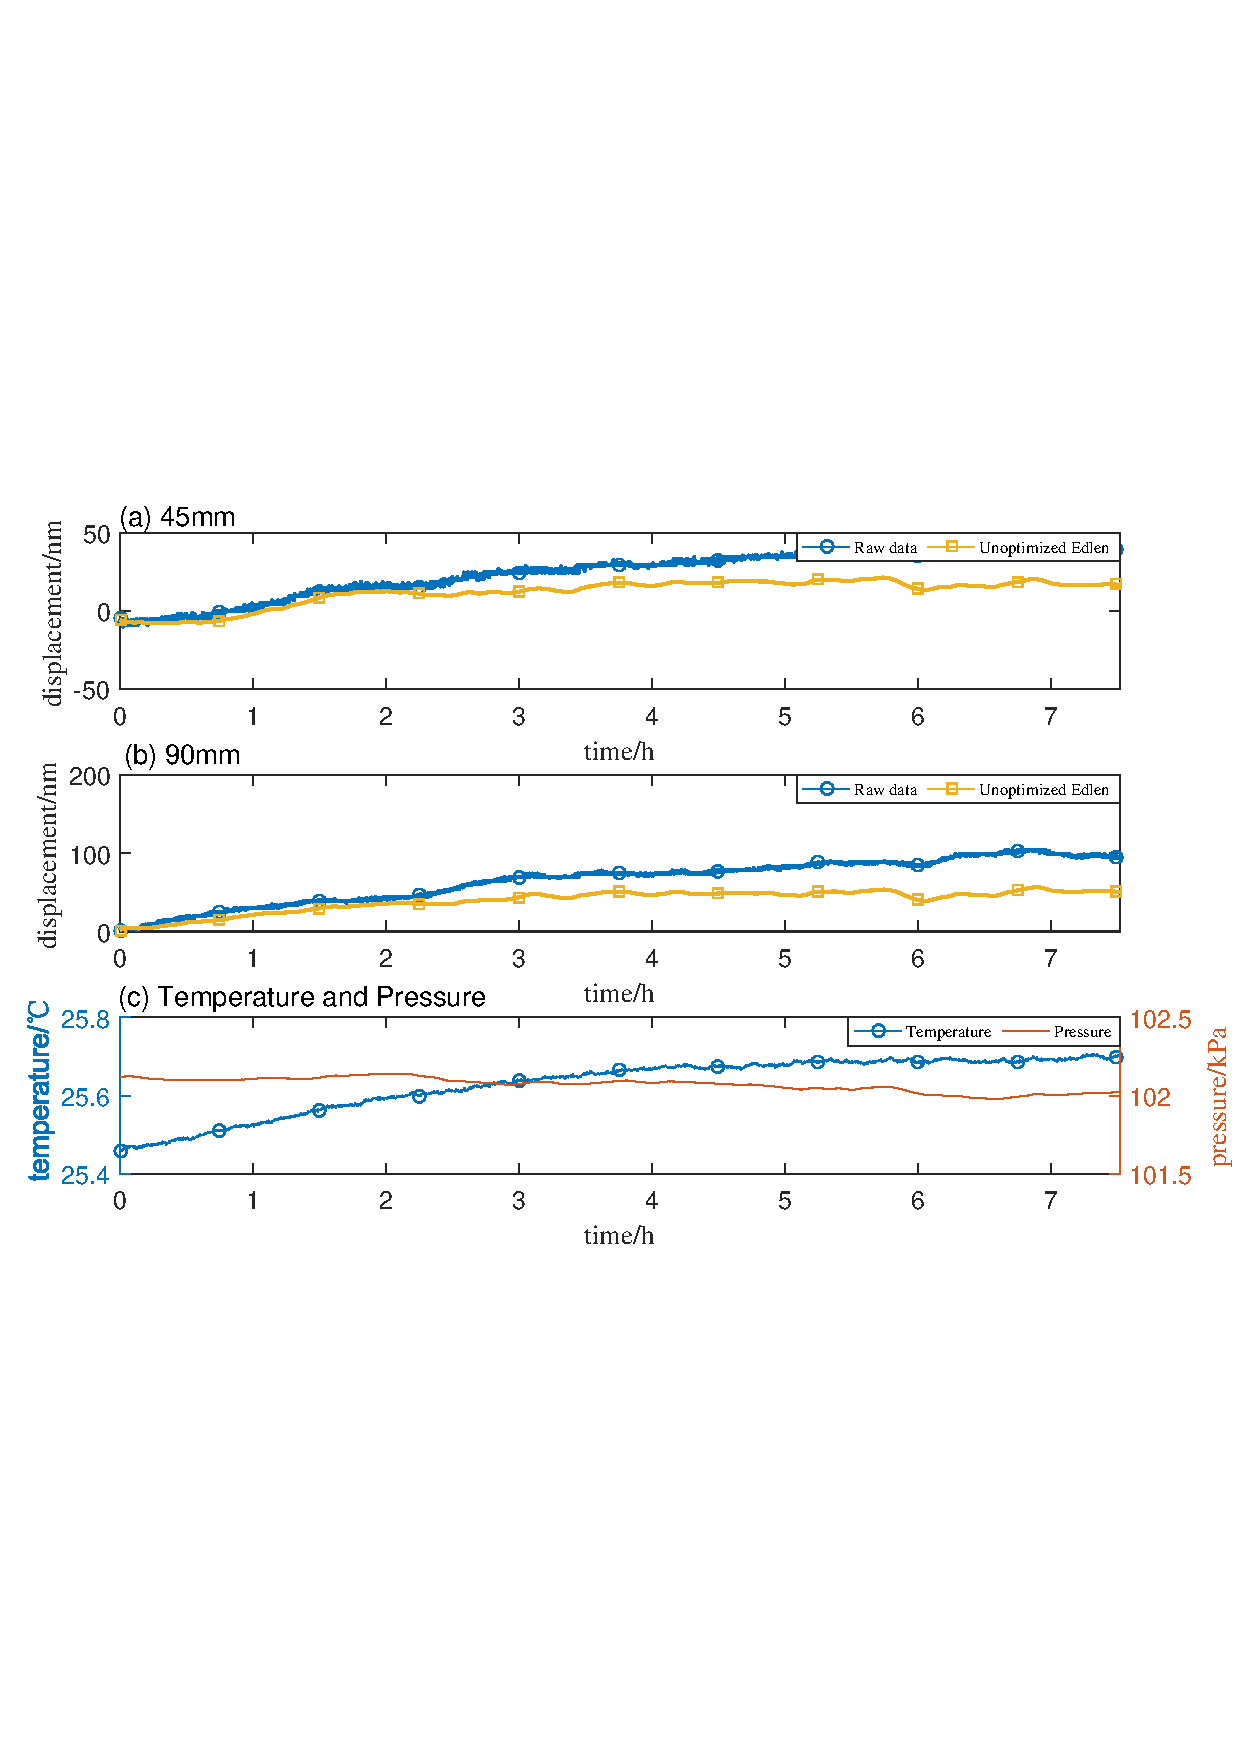
\includegraphics[width=14cm]{fig/3-fig/长时测量数据.pdf}
  \caption{长时测量实验数据}
  \label{fig:长时测量实验数据}
\end{figure}

从图中可以看出,测量时间约为$7.5h$,温度变化范围为$[25.46\,\,\,25.69]^{\circ}C$,气压变化范围为$[102.0\,\,\,102.1]kPa$,测量臂长度为$45nm$和$90nm$的两套干涉仪的原始位移数据的变化范围为$[0\,\,\,35.62]nm$和$[0\,\,\,89.01]nm$,在考虑可能含有随机误差等其他误差的情况下,可近似认为两者成两倍关系。并且对于零位测量而言,上述位移变化都可以认为是误差,对应的均方根误差分别为$30.5299nm$和$75.0362nm$,经过Edlen公式补偿后的均方根误差为$14.9957nm$和$41.9108nm$,补偿效果约为$50.8\%$和$45\%$。

可以看出在进行长时间测量的情况下使用Edlen公式进行干涉仪的环境误差补偿也可以取得一定的补偿效果,但是补偿效果并没有短时测量的效果好,应是测量时间增长使得温度、气压、位移的累计测量误差变大导致,除此之外,仍可以发现补偿后的残留均方根误差依旧有一定差距,补偿效果有提升空间。

\subsection{大范围温度变化测量}
为了更加验证原始Edlen公式由于其温度不匹配问题造成的使用局限性,将测量时温度温度设置的更加远离Edlen公式的提出温度$20^{\circ}C$,并且增大温度变化区间,进一步增加测量时间,得到的实验数据如图\ref{fig:大范围温度测量实验数据}。
\begin{figure}[htb]
    \centering
    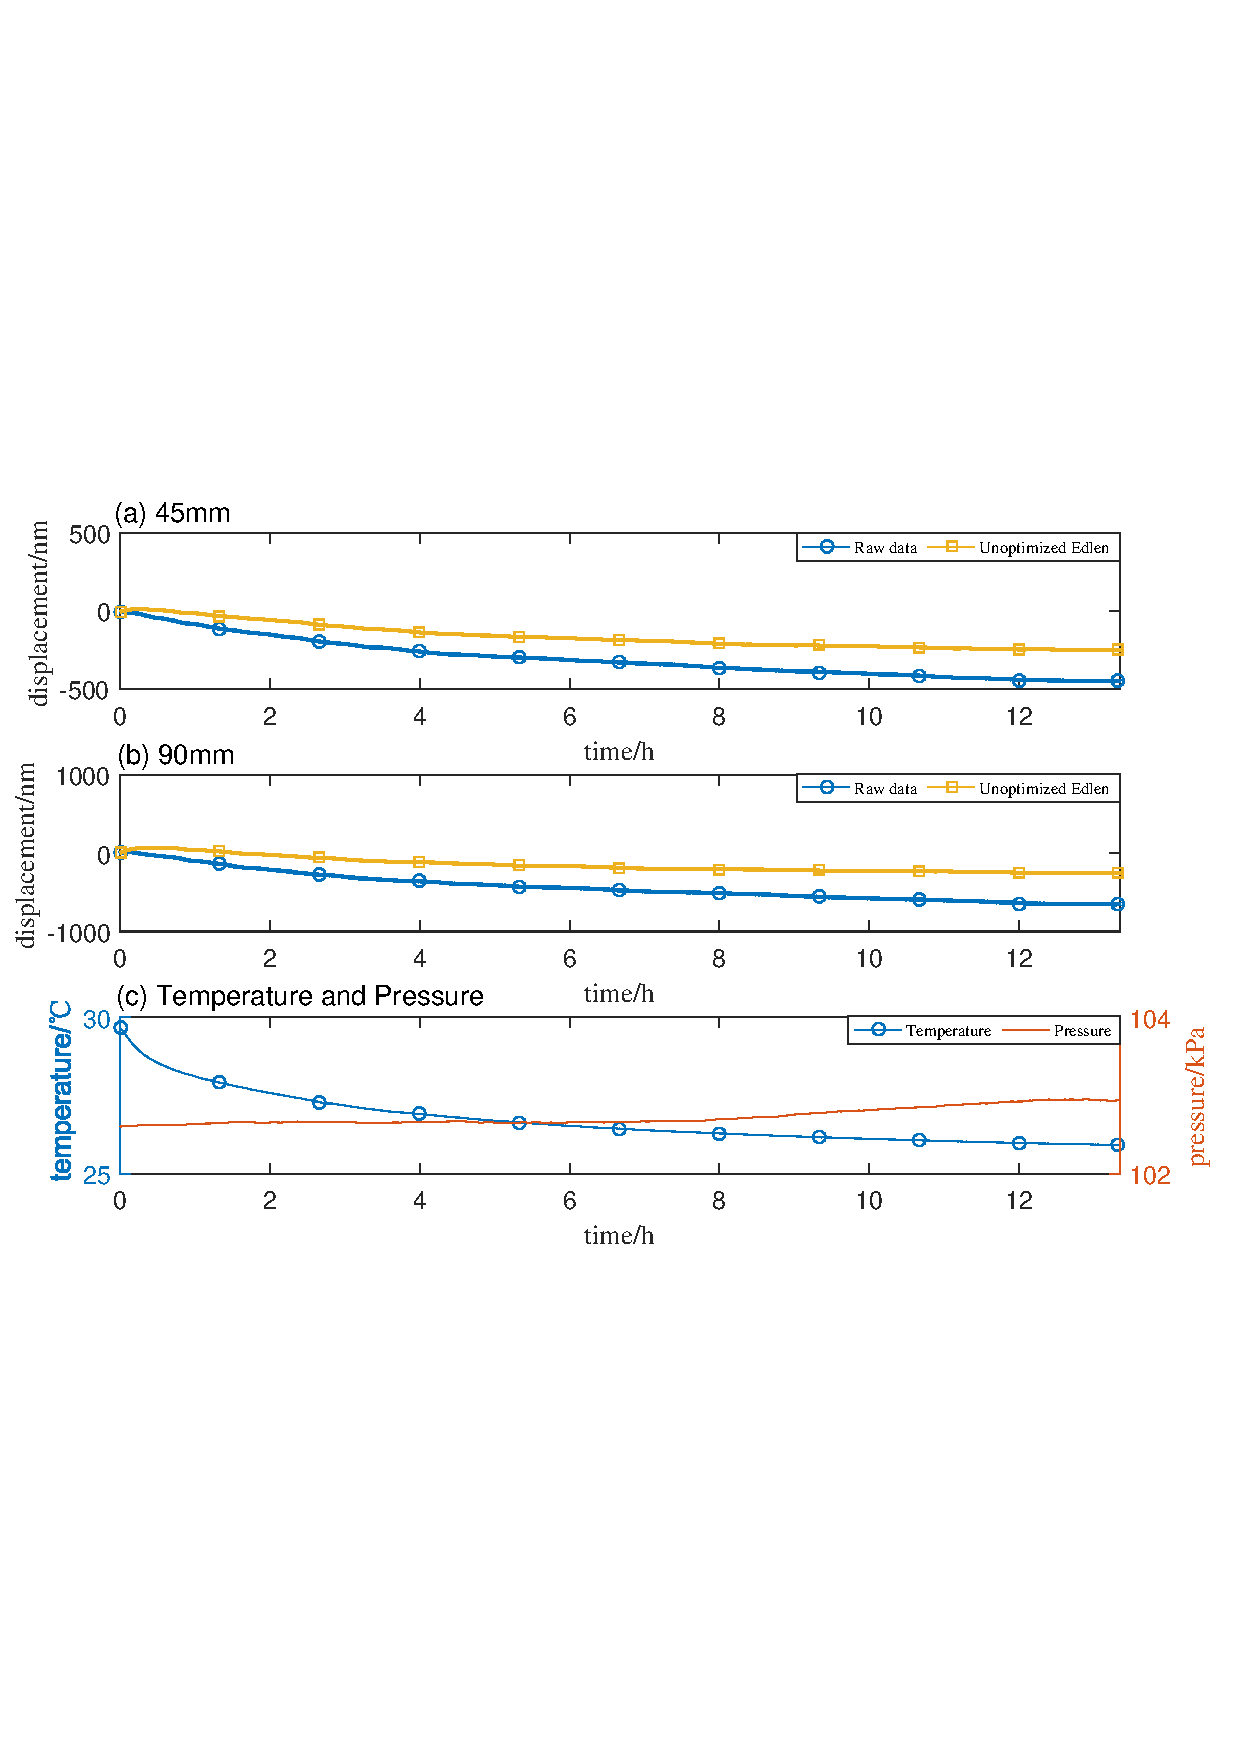
\includegraphics[width=14cm]{fig/3-fig/大范围温度测量实验数据.pdf}
    \caption{大范围温度测量实验数据}
    \label{fig:大范围温度测量实验数据}
  \end{figure}
从图中可以看出,测量时间约为$12.5h$,温度变化范围为$[25.91\,\,\,29.67]^{\circ}C$,气压变化范围为$[102.6\,\,\,102.9]kPa$,测量臂长度为$45nm$和$90nm$的两套干涉仪的原始位移数据的变化范围为$[0 \,\,\, -248.3]nm$和$[0\,\,\,-652.8]nm$,在考虑可能含有随机误差等其他误差的情况下,可近似认为两者成两倍关系。并且对于零位测量而言,上述位移变化都可以认为是误差,对应的均方根误差分别为$325.0990nm$和$465.0772nm$。经过Edlen公式补偿后的均方根误差为$153.6245nm$和$176.6071nm$,补偿效果约为$53\%$和$62\%$。

可以看出使用Edlen公式进行干涉仪的环境误差补偿可以得到较好的补偿效果,但是经过Edlen公式补偿之后的残留均方根误差仍有较大差距,并且相比于短时测量的差值$2.7024nm$而言,由于温度更加远离$20^{\circ}C$,并且温度变化范围也更大了,导致残留误差的差值也增大到了$22.983nm$,再次验证了温度不匹配导致原始Edlen公式的补偿效果降低。

从图中还可以看出,在前$0.8h$的测量时间段内,经过Edlen公式补偿后的值有一个正向的凸起,高度约为$70nm$(测量臂长度$90nm$的数据),而干涉仪的位移测量值一直都是处于负数范围内,此时补偿结果的变化趋势是与干涉仪位移值的变化趋势相反的,即由于进行了补偿,导致干涉仪的位移值从负数跨越零点达到正数,并且距离零点有一点距离,这说明发生了过补偿的现象。但在剩余$12h$的测量时间内,补偿结果的变化趋势是与干涉仪位移值的变化趋势都是相同的(即变小)。从(c)图中可以看出,前$0.8h$时间内,测量温度是最远离Edlen公式的提出温度$20^{\circ}C$,这段时间内发生过补偿进一步说明了温度不匹配造成Edlen公式补偿效果的下降。而且这$0.8h$内温度从$29.67^{\circ}C$减小到了$28.22^{\circ}C$,即在约$6.4\%$的时间内,完成了约整个过程约$38.6\%$的温度变化,这一数据说明,当温度梯度过大时,可能会对干涉仪的位移测量引入其他误差,这部分将在下文介绍。

\section{本章小结}
本章主要介绍了实验设备的组成,包括:双频激光干涉仪的光路设计及其分析、基于PT100的多通道温度测量系统,包含其上位机软件以及标定过程和标定结果、PACE1000气压传感器。并介绍了部分不太完善的实验方案及其结果分析,从实验设备、实验变量、实验环境以及实验方法四个方面不断改进,并得到最终的实验方案,并进行了短时测量、长时测量等对照实验,从具体的数据分析验证了Edlen公式在波长不匹配、温度范围不匹配的情况下,仍然能对干涉仪的环境误差进行一定程度的补偿,但会有一定的性能损失。
  
\chapter{基于粒子群算法的软件补偿方法及算法硬化}
\section{粒子群算法}
\label{粒子群算法}
\subsection{粒子群算法基本原理}

粒子群算法(Particle Swarm optimization,PSO)是一种启发于鸟群协同捕食行为的智能算法,利用种群与个体之间的信息交互来寻找问题的最优解,具有较高的搜索效率和精度\cite{潘红丽2022基于改进粒子群算法的垃圾清运车辆低碳路径规划},已广泛应用于函数优化等领域\cite{2022Environmental}。
\begin{figure}[htb]
  \centering
  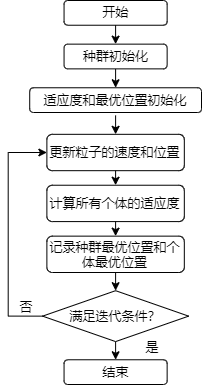
\includegraphics[width=4cm,height=7cm]{fig/4-fig/粒子群算法流程图.png}
  \caption{粒子群算法流程图}
  \label{fig:粒子群算法流程图}
\end{figure}

可以假设这样一个场景:一群鸟在随机的搜寻食物,并且搜寻空间里只有一块食物,所有的鸟都不知道食物在哪里,并且所有鸟的初始位置和搜寻方向都是随机的。在该场景下,一个找寻食物的最优策略就是搜寻离食物最近的鸟的周围。距离食物的距离就代表着优化效果的好坏,而鸟群每个时刻所处在的位置,就代表着粒子群算法覆盖到的迭代值,整个空间即为粒子群算法的搜索空间,将该方式抽象成算法,如图\ref{fig:粒子群算法流程图}所示。

由图\ref{fig:粒子群算法流程图}中可以看出,粒子群算法的第一步是对种群进行初始化,即设定优化对象的迭代起点,并根据目标函数计算出与起点对应的适应度(Fitness,下文简称fit),并在所有个体的适应度中筛选出最优的,用其对应的迭代起点作为整个种群目前的种群最优解(Global best,下文简称gbest),而所有个体的个体最优解(Person best,下文简称pbest),这样就完成了整个算法的初始化。随后使用gbest、pbest对粒子的速度和位置更新进行控制,使迭代方向不断朝着最优的方向进行,即上述“搜寻离食物最近的鸟的周围”的策略,具体的速度更新公式和位置更新公式如下式所示:
\begin{equation}\label{eq:粒子群算法速度更新}
  V^{k+1}_i=\omega V^{k}_i\,+\,c_pr_{and}(pbest_i-X^{(k)}_i)+c_gr_{and}(gbest\,-\,X^{(k)}_i).
\end{equation}
\begin{equation}\label{eq:粒子群算法位置新}
    X^{k+1}_i\,=\,X^{(k)}_i\,+\,V_i^{k+1}.
\end{equation}

上式中\(V^{k}_i\)和\( X^{k}_i\)中分别表示粒子的速度和位置,下标i表示种群中第i个粒子,上标(k+1)表示当前种群为第(k+1)次迭代,\(\omega\)称为惯性因子,是一个衡量全局寻优能力和局部寻优能力的非负参数;\(c_p\)和\(c_g\)为非负常数,通常设为2;、\(r_{and}\)为[0,1]范围内的随机数,\(pbest_i\)为第个粒子的个体历史最优位置,gbest为整个种群的历史最优位置。

\subsection{线性惯性权值递减策略}
由式\eqref{eq:粒子群算法速度更新}可以看出惯性因子主要控制粒子的历史速度对当前速度的影响,历史速度在当前速度中占比大,则速度的更新将主要集中在历史速度附近,此时粒子群算法的局部寻优能力较强,并且收敛速度较快;若历史速度在当前速度中占比小,则速度的更新将在整个搜索域中进行,此时粒子群算法的全局寻优能力较强,使得搜索结果容易跳出局部优值。

为了在迭代初期,能够有更好的全局寻优能力,尽可能找到搜索域中所有可能的最优解,在迭代后期拥有更好的局部寻优能力,以便快速收敛,在惯性因子的取值上采用线性递减策略\cite{冯浩2015一种改进的粒子群优化算法惯性权值递减策略},即惯性因子\(\omega\)由下式更新。
\begin{equation}\label{eq:omega更新公式}
  \omega^k\,=\,\omega_e\,+\,\frac{(\omega_i\,-\,\omega_e)(k_{max}\,-\,k)}{k_{max}}.
  \end{equation}

其中\(\omega_i\)和\(\omega_e\)分别为迭代开始时的惯性因子和迭代结束时的惯性因子,\(k_{max}\)为最大迭代次数,k为当前的迭代次数。通过对惯性因子使用线性递减策略,可以在迭代过程中不断调整全局寻优能力和局部寻优能力。

但是粒子群算法存在早熟收敛的问题,即当粒子群到达局部最优解附近时,粒子速度的更新主要由自身速度决定,并且由于粒子群算法的惯性因子\(\omega^k\)通常小于1,使得粒子速度的更新幅度将会越来越小,难以跳出该局部最优解\cite{范培蕾2009克服早熟收敛现象的粒子群优化算法}。

虽然Edlen公式的诞生方法使其补偿精度和使用条件受到一定影响,但原始的Edlen公式为PSO算法提供了一个优秀的搜索起点,相当于大幅压缩了PSO算法的搜索空间,这能非常有效地避免早熟收敛问题的出现。

\section{基于粒子群算法优化后的Edlen公式补偿方法}
为了解决上述的Edlen公式存在的问题,本文提出一种使用粒子群算法对Edlen公式进行优化的方法。

对于粒子群算法而言,目标函数的形式会严重影响算法优化的结果,而Edlen公式作为一个几十年来广泛使用的经验公式,虽然由于其诞生条件的局限性使得其使用范围受限,但Edlen公式的形式仍然具有重要的借鉴意义,将Edlen公式与粒子群算法相结合,不仅可以有效地避免粒子群算法寻找到局部最优解,避免早熟收敛现象的发生,还可以减小搜索空间,减小收敛时间,保证训练时不会影响实时数据测量及补偿。
\subsection{数据预处理}
使用粒子群算法对Edlen公式进行优化的第一步是对位移、温度、气压数据进行预处理,这点主要是基于下面两点考虑:
\begin{enumerate}
  \item 虽然所有被测量的采样周期均为$2s$,但是由于位移测量的上位机采用C-SHOP编写,而温度测量的上位机是基于LabVIEW开发的,气压测量主要依靠PACE1000气压传感器,这导致三者在定时功能上可能会有细微差别,而导致最终采样的点数不相同,所需要进行数据的裁剪。
  \item 出于不漏采任何有效信息,所以将采样周期设置为$2s$,但是温度和气压都是缓变量,并不可能在这么短的时间内明显变化,所以为了数据的可靠性,避免偶然性数据造成训练效果降低,需要对数据进行均值滤波。
\end{enumerate}
在进行数裁剪的时候采用如下策略:将位移、温度、气压三组中数据个数最少的作为基准,计算另外两组数据个数与基准的差值,这个差值即为需要裁剪的数据个数,将数据个数除以裁剪个数,然后向下取整即可得到每组数据对应的裁剪窗口长度,在每个裁剪窗口内将最后两个数取平均值,用平均值代替这两个数,这样即可实现数据裁剪。

在进行均值滤波的时候采用如下策略:取窗口长度为$30s$,即15个数据点,在整个数据段内进行滑动窗口的均值滤波。

\subsection{使用粒子群算法进行数据训练}
将式\eqref{eq:线性形式的Edlen公式}作为粒子群算法的目标函数,温度因子$\frac{\delta n}{\delta T}$和气压因子$\frac{\delta n}{\delta P}$作为两个搜索目标,第一次迭代的搜索起点分别为$-9.36*10^{-7}$和$2.68*10^{-9}$,即搜索点由下式更新:
\begin{equation}\label{eq:搜索点更新公式}
  \delta^{(n+1)}_i = \delta^{(n)}_i+(\delta^{(n)}_o-\delta^{(n)}_i).
  \end{equation}

式\eqref{eq:搜索点更新公式}中$\delta^{(n+1)}_i$为第$n+1$次训练时温度因子、气压因子初始搜索点,即$\delta_i\,=\,(\frac{\delta n}{\delta T}\,\,\,\frac{\delta n}{\delta P})$,所以该式描述的是第$n+1$的搜索起点与第$n$次搜索起点之间的关系。特别地,当$n=0$时,即第一次搜索的搜索起点为$\delta_i\,=\,(-9.36*10^{-7}\,\,\,2.68*10^{-9})$,即原始Edlen公式的温度因子值和气压因子值。$\delta_o^{(n)}$为第$n$次训练后粒子群算法计算出的温度因子和气压因子。

而每次训练计算$\delta_o^{(n)}$的适应度时,采用均方根误差作为评价指标,其计算方法如式\eqref{eq:均方根误差计算公式}所示:

\begin{equation}\label{eq:均方根误差计算公式}
  RMSE = \sqrt{\frac{\sum_{i=1}^{N}(x-\widehat x)^2}{N}}.
  \end{equation}


\section{整段式粒子群算法补偿效果}
将一整组的测量数据作为粒子群算法的训练样本,从给定的搜索起点开始,根据式\eqref{eq:均方根误差计算公式}计算初始适应度,并且进行种群最优位置和个体最优位置的初始化,然后根据式\eqref{eq:粒子群算法速度更新}和式\eqref{eq:粒子群算法位置新}更新种群中所有个体的速度和位置,然后循环迭代多次,直至达到迭代次数上限,此时种群的最优位置即为粒子群算法优化后的Edlen公式中的温度因子和气压因子,然后对测量数据进行补偿。训练样本统一使用测量臂长度$90nm$的干涉仪的测量数据,使用优化结果对测量臂长度$45nm$和$90nm$测量数据同时进行补偿,补偿结果如下。

\subsection{短时测量}
如图\ref{fig:粒子群算法优化后的短时测量补偿效果}所示,(a)图为测量臂长度为$45nm$的位移测量数据,(b)图为测量臂长度为$90nm$的位移测量数据,(c)图为对应的温度和气压数据,(a)、(b)、(c)三图的横轴均为时间,单位为h;(a)和(b)图中的竖轴为位移数据,单位为$nm$,其中带圆圈标注的蓝色曲线为原始的位移测量数据,带黄色方块标注的为使用原始Edlen公式补偿后的位移数据,带红色菱形标注的为使用粒子群算法优化后的补偿后位移数据,(c)图的竖轴为温度和气压数据,单位为$^{\circ}C$和$kPa$,其中带圆圈标注的蓝色曲线为温度数据,红色曲线为气压数据。
\begin{figure}[htb]
    \centering
    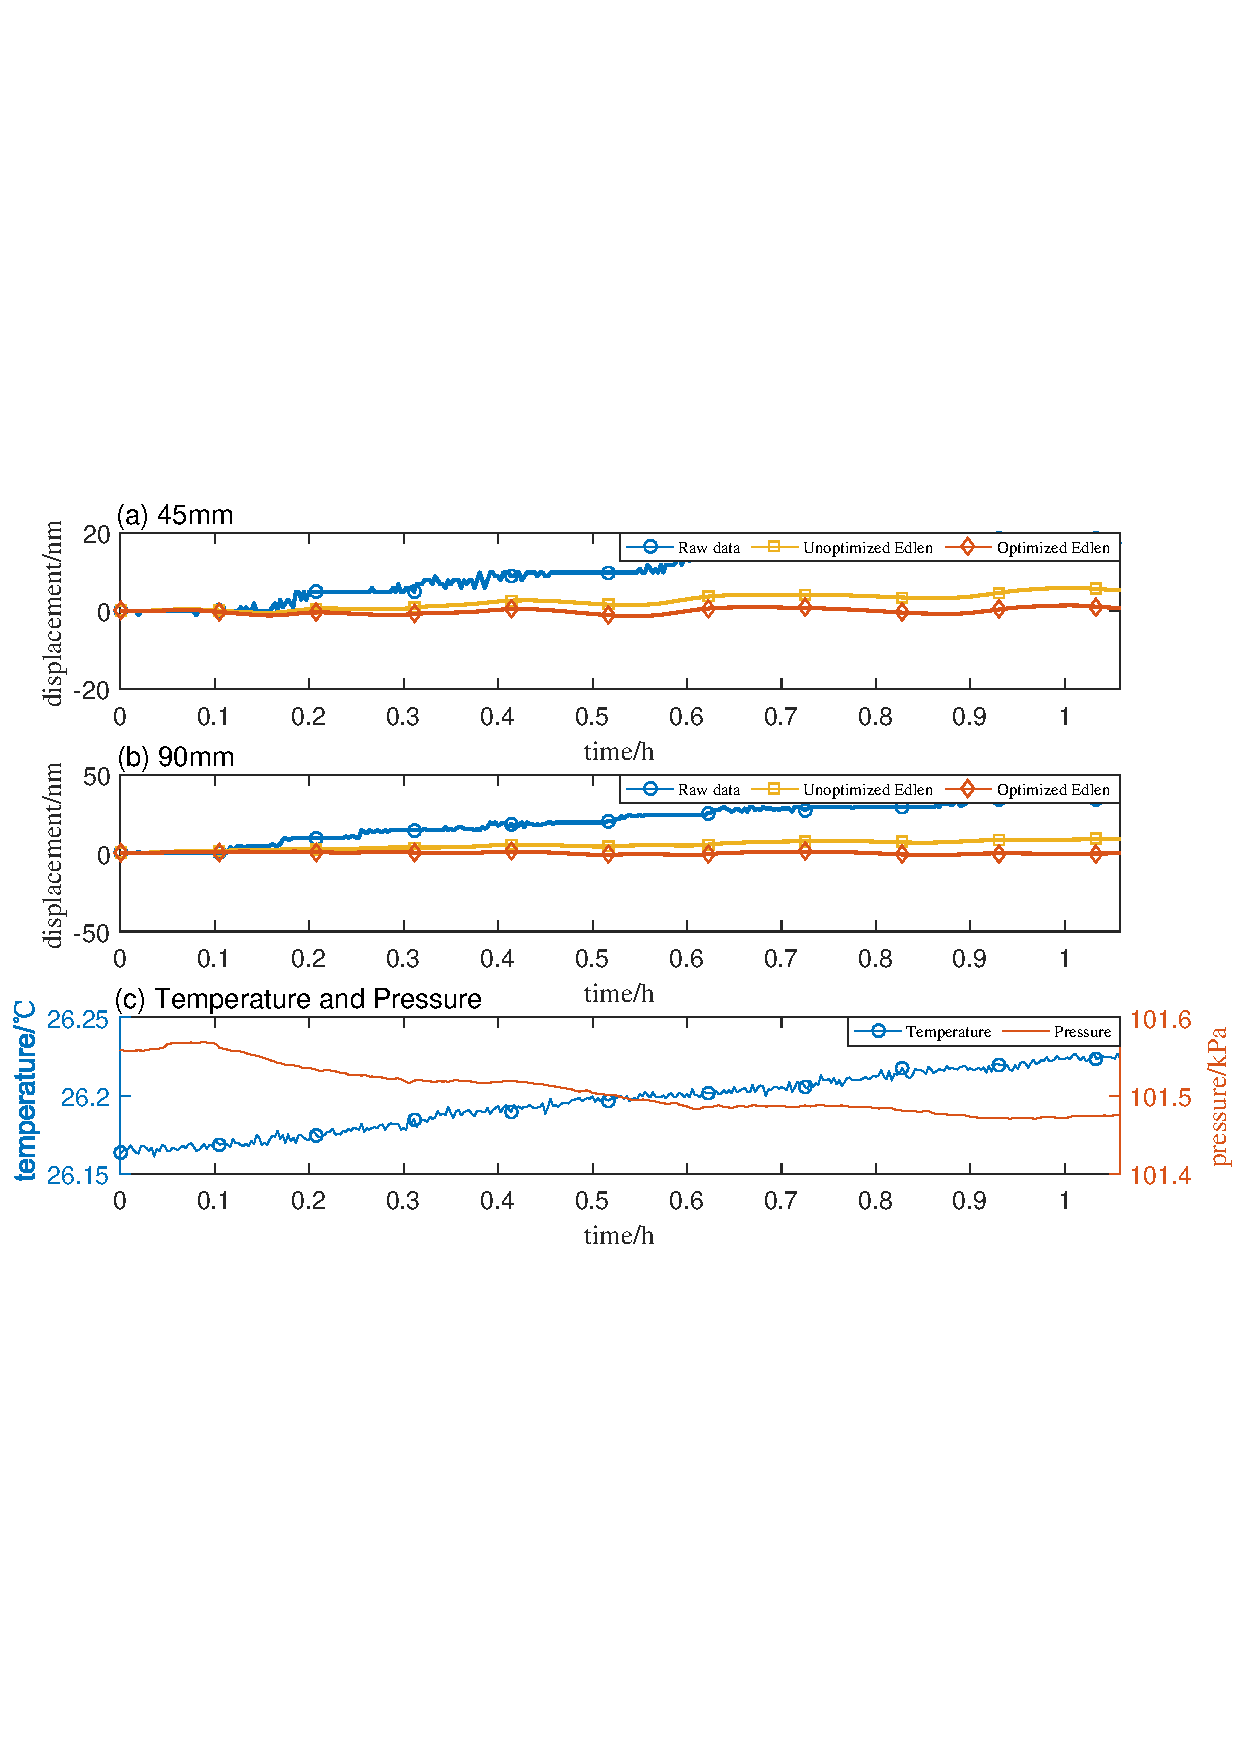
\includegraphics[width=14cm]{fig/4-fig/edpso_短时测量实验数据.pdf}
    \caption{粒子群算法优化后的短时测量补偿效果}
    \label{fig:粒子群算法优化后的短时测量补偿效果}
\end{figure}

如图\ref{fig:粒子群算法优化后的短时测量补偿效果}所示,优化后的红色曲线相比于未经优化的黄色曲线,无论是$45nm$还是$90nm$情况下,都更加接近于理论位移值$0nm$,这说明使用粒子群算法对Edlen公式进行优化之后在进行补偿可以比较明显地提升补偿效果。从数据层面分析,使用粒子群算法进行优化之后再进行补偿,测量臂长度为$45nm$的干涉仪的残留均方根误差从$3.1377nm$降低为$0.8541nm$,而$90nm$长度的则从$5.8401nm$降低为$1.034nm$,分别同比减小了$72.7\%$和$82.3\%$,并且两者残差的差值只有$0.1799nm$,相较于未优化前的差值$2.7024nm$有着较大提升,可以认为使用经过粒子群算法优化之后的Edlen公式进行补偿后的残差在不同测量臂长度情况下是近似相等的,这说明环境误差得到了比较精准并且完全的补偿。但是如果从百分比的角度分析,$0.1799nm$的残差差值占原始残差的比例约为$21\%$,这是一个比较大的百分比,可能的原因是由于改组温度变化较小,使得环境误差在总体误差中的比例不够大。

\subsection{长时测量}
对前文所述的长时测量的实验数据也是用粒子群算法优化后再进行补偿,结果如图\ref{fig:粒子群算法优化后的长时测量补偿效果}所示,虽然采样时长增加了,但是粒子群算法的优化效果依旧显著。从数据层面分析,使用粒子群算法进行优化之后再进行补偿,测量臂长度为$45nm$的干涉仪的残留均方根误差从$14.9957nm$降低为$6.8308 nm$,而$90nm$长度的则从$43.5806nm$降低为$3.6700nm$,两者残差的差值只有$3.16nm$,相较于未优化前的差值$28.5849nm$有着较大提升,可以认为使用经过粒子群算法优化之后的Edlen公式进行补偿后的残差在不同测量臂长度情况下是近似相等的,这说明环境误差得到了比较精准并且完全的补偿。
\begin{figure}[htb]
  \centering
  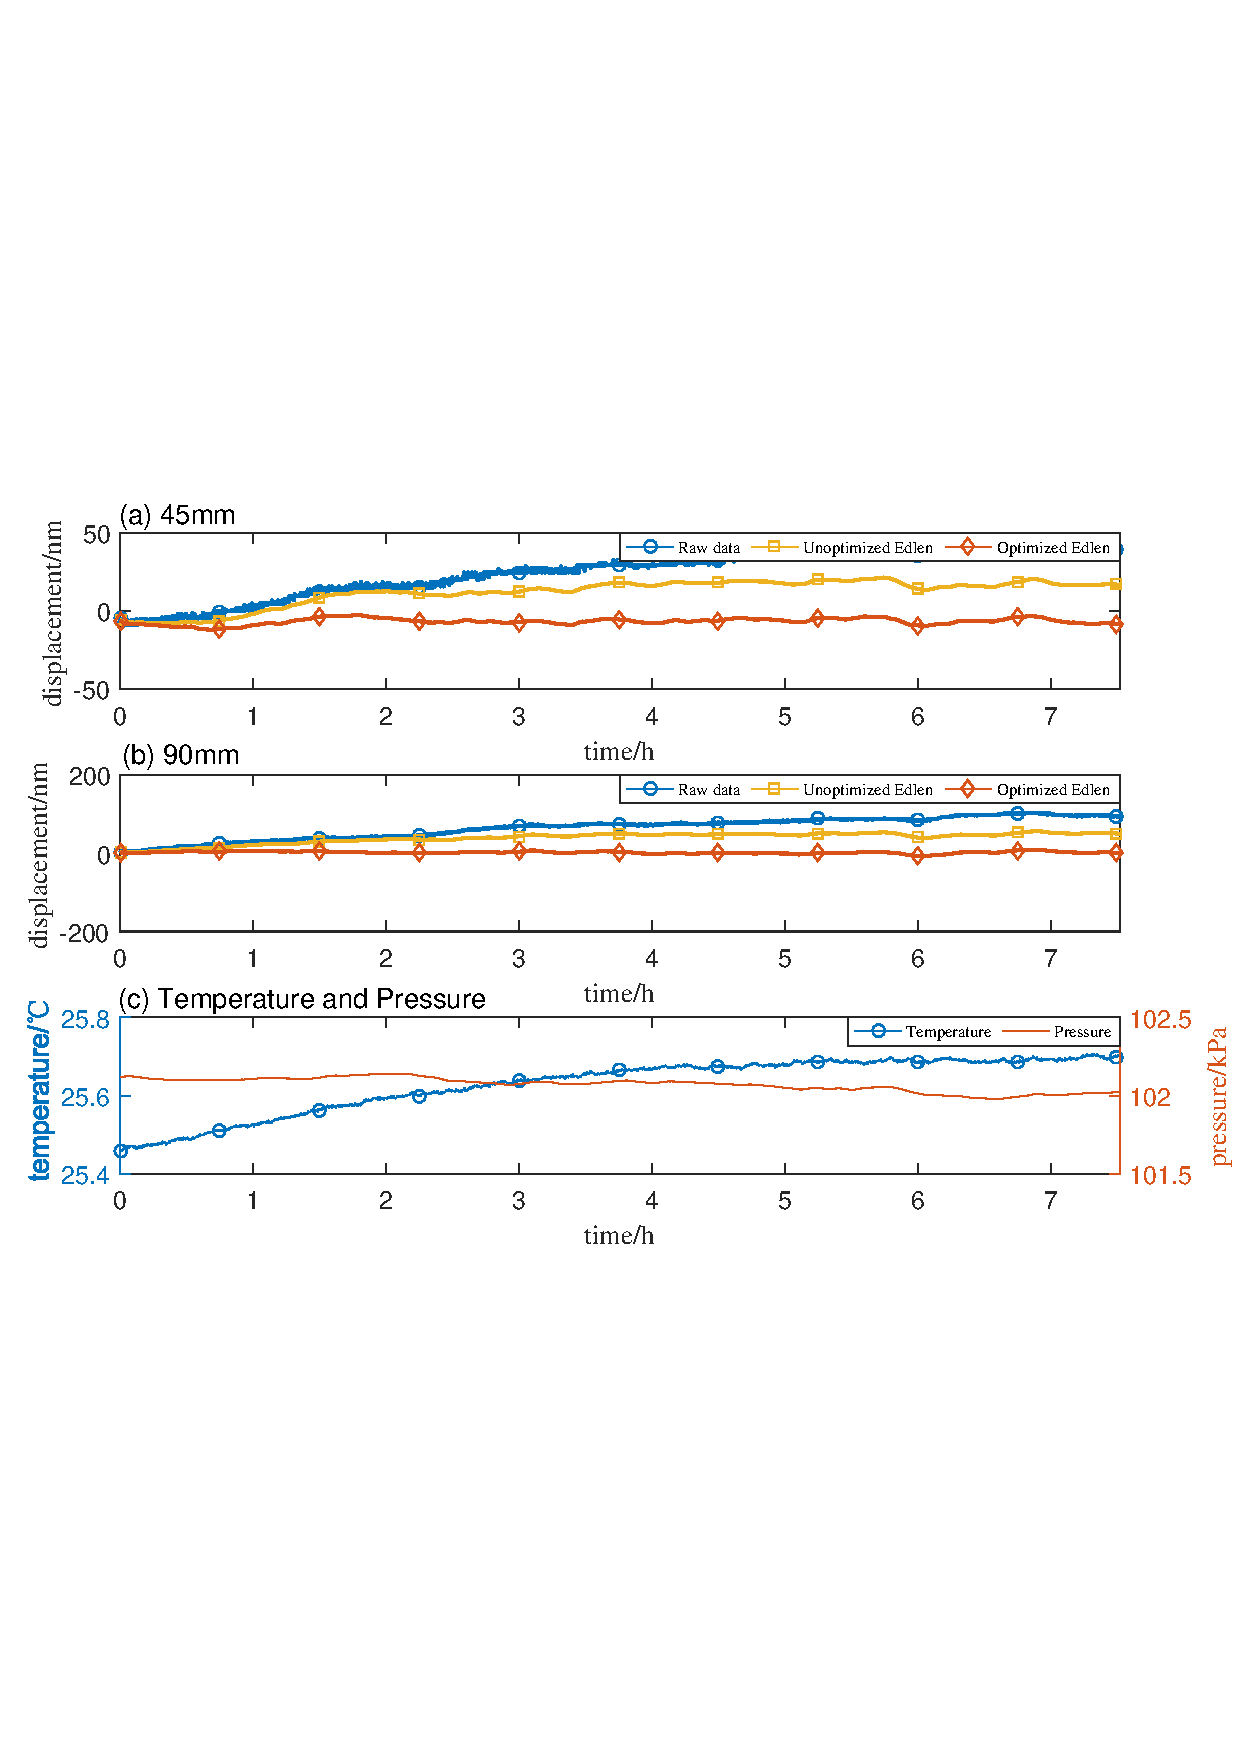
\includegraphics[width=14cm]{fig/4-fig/edpso_长时测量实验数据.pdf}
  \caption{粒子群算法优化后的长时测量补偿效果}
  \label{fig:粒子群算法优化后的长时测量补偿效果}
\end{figure}

同时,从数据中可以发现,测量臂长度为$90nm$的数据经过粒子群算法优化后的补偿残差$3.6700nm$是小于$45nm$的$6.8308nm$,可能原因有:
\begin{enumerate}
  \item 由于粒子群算法在训练过程中使用的是$90nm$的测量数据,并且该组试验的测量时间较长,使得粒子群算法较好地挖掘了数据中潜在的规律,达到比较完美的补偿效果。
  \item $45nm$的测量数据发生了过补偿。
  \item 由于环境补偿后的残差较小,所以可能由于随机误差的干扰。
\end{enumerate}

需要特别说明的是,从其他未给出的实验数据以及下文给出的大范围温度变化测量的结果分析,比较大的可能是由于随机误差的干扰。
\subsection{大范围温度变化测量}
对前文所述的大范围温度变化测量的实验数据也是用粒子群算法优化后再进行补偿,结果如图\ref{fig:粒子群算法优化后的大范围温度变化测量补偿效果}所示,虽然采样时长以及温度变化范围都增加了,但是粒子群算法的优化效果依旧显著。从数据层面分析,使用粒子群算法进行优化之后再进行补偿,测量臂长度为$45nm$的干涉仪的残留均方根误差从$153.6245nm$降低为$29.3458 nm$,而$90nm$长度的则从$176.6071nm$降低为$48.4996nm$,两者残差的差值仍有$19.1538nm$,相较于未优化前的差值$28.5849nm$有着一定提升,这说明环境误差的补偿效果得到一定改善,但是不同测量臂长度下的残差仍然不可以认为是相等的,说明该组实验数据哪怕经过整段式粒子群算法的优化,其补偿效果也只是提升了,并未像前两组实验数据那样得到精准且完全的补偿。
\begin{figure}[htb]
  \centering
  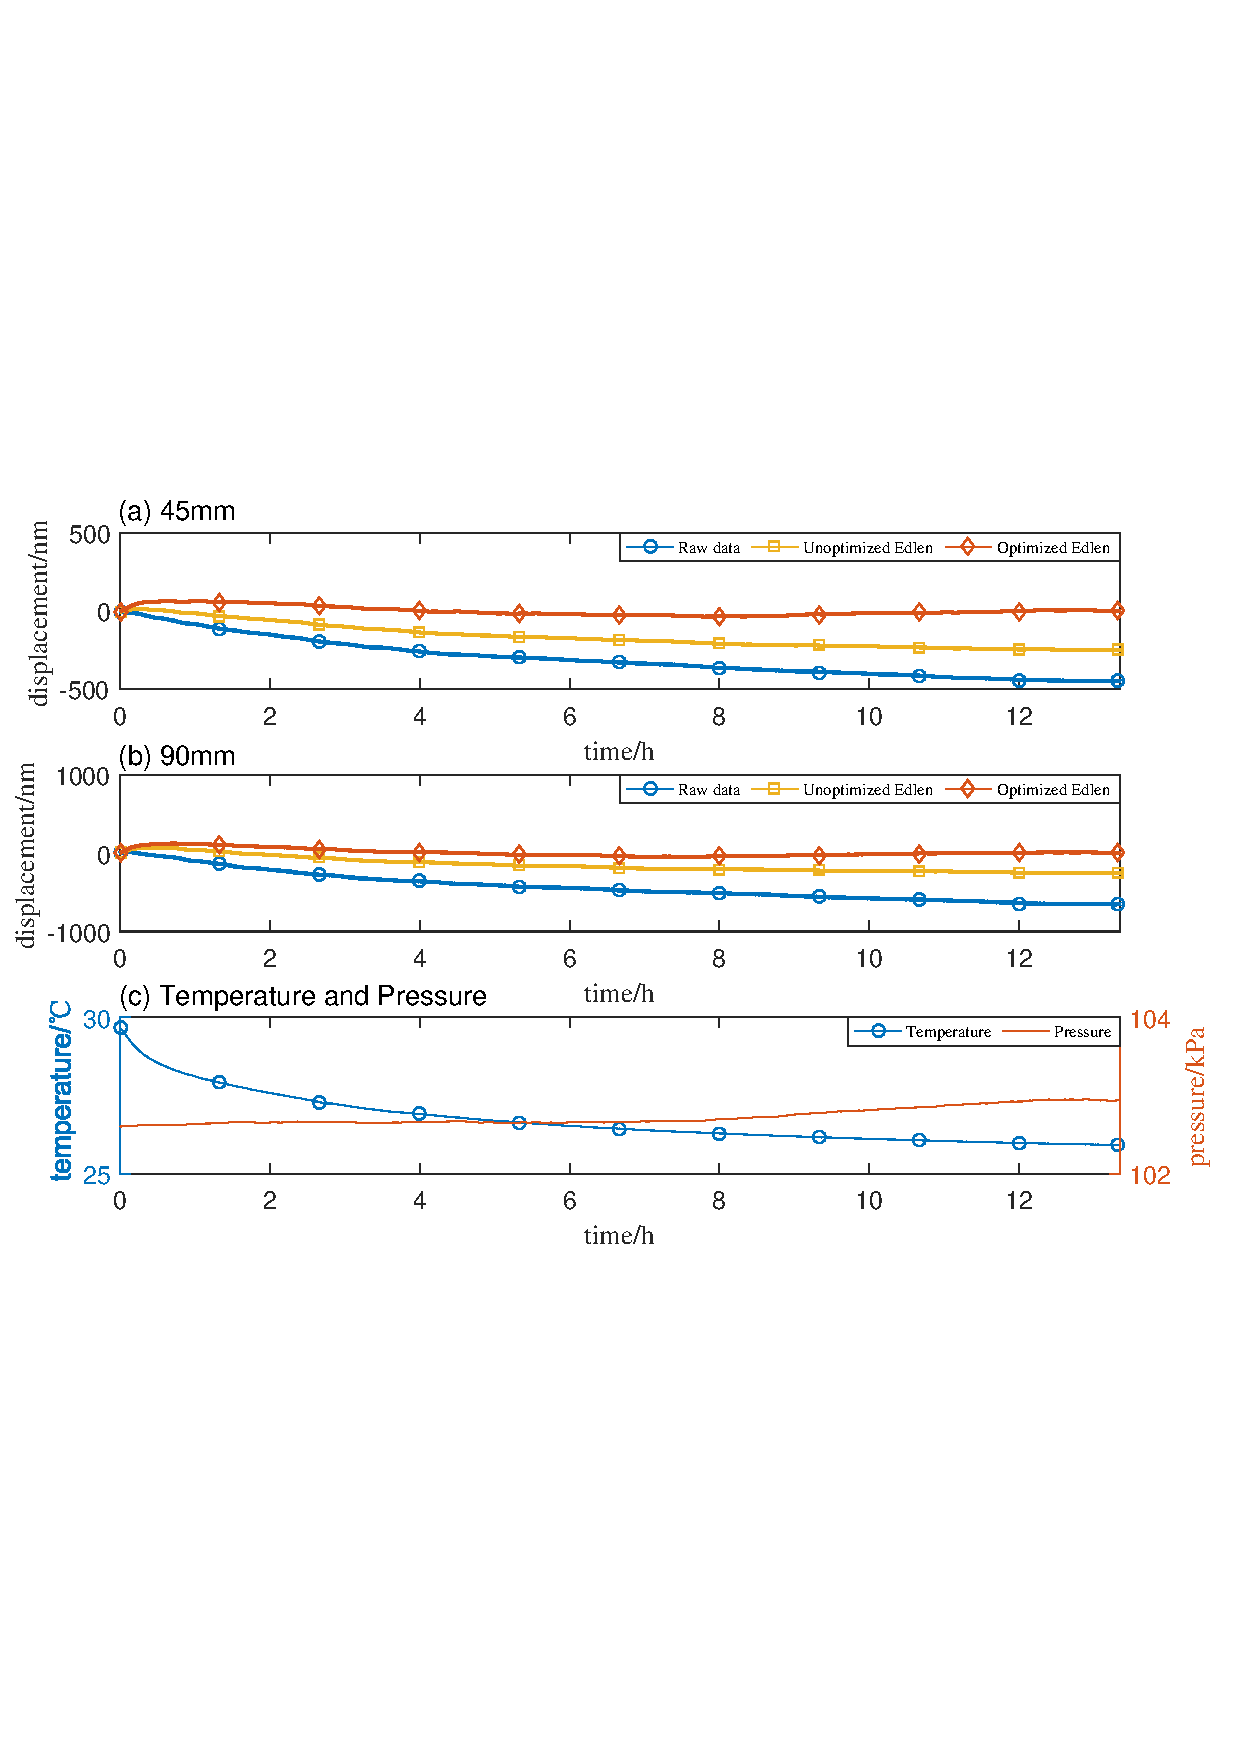
\includegraphics[width=14cm]{fig/4-fig/edpso_大范围温度变化测量数据.pdf}
  \caption{粒子群算法优化后的大范围温度变化测量补偿效果}
  \label{fig:粒子群算法优化后的大范围温度变化测量补偿效果}
\end{figure}

但是从上述的分析数据中可以看出,该组的温度变化以及测量时间均比长时测量实验中长,但是经过粒子群算法优化后再进行补偿得到的残差值,并未出现长时测量实验中:测量臂长度为$45nm$的补偿残差大于测量臂长度为$90nm$的补偿残差,这进一步验证了长时测量实验中出现该现象的原因是由于偶然的随机误差,难以复现。

前$0.8h$时间内的过补偿现象变得更严重了,经粒子群算法优化后的补偿结果的凸起高度从$70nm$增大到了约$120nm$,但是使用粒子群算法优化后在整个$12.5h$测量时间内的补偿效果是改善的,这说明粒子群算法已经比较完全地挖掘出了Edlen公式的补偿性能,只是在大温度梯度的情况下,可能引入了其他误差因素,导致线性形式的Edlen公式无法适用。

\subsection{优越性}
上述的实验结果可以说明,将Edlen公式与粒子群算法相结合,可以比较有效地减小Edlen公式本身温度不匹配、波长不匹配的问题,提高补偿效果。但在\ref{粒子群算法}节中也说明了,将Edlen公式与粒子群算法相结合,也可以很有效地避免粒子群算法自身早熟收敛的问题。如图\ref{fig:粒子群算法训练过程}所示,图\ref{fig:以Edlen公式为起点的训练过程}为以Edlen公式为搜索起点的三次训练过程数据,而图\ref{fig:以零点为起点的训练过程}为以零点为搜索起点的三次训练过程数据,最大迭代次数均为150次。可以明显看出,若以Edlen公式为搜索起点,三次训练结果都能准确落在同一位置,对应的适应度为0.06861,可以认为是找到了全局最优解;而若从零点开始搜索,三次训练结果落在了三个不同位置,对应的适应度分别为0.07031、0.06861、0.08587,只有一次找到了全局最优解,而另外两次都只找到了局部最优解,并且最少又经历了40次迭代都没有跳出这个局部最优解,发生了早熟收敛现象。

\begin{figure}[htb]
  \centering
  \subfigure[以Edlen公式为起点的训练过程]{
    \begin{minipage}[b]{0.99\textwidth}
      \centering
      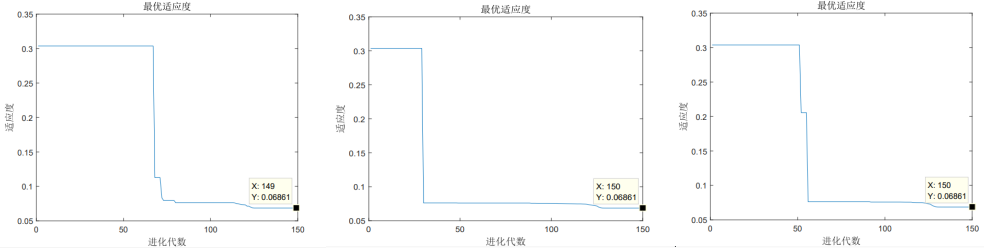
\includegraphics[width=14cm,height=5cm]{fig/4-fig/训练过程a.png}
    \end{minipage}
    \label{fig:以Edlen公式为起点的训练过程}
  }
  \subfigure[以零点为起点的训练过程]{
    \begin{minipage}[b]{0.99\textwidth}
      \centering
      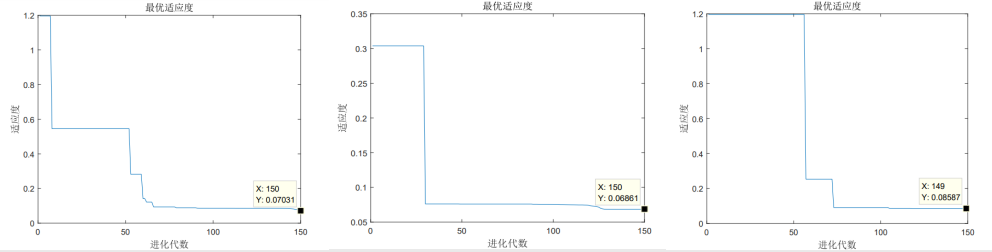
\includegraphics[width=14cm,height=5cm]{fig/4-fig/训练过程b.png}
    \end{minipage}
    \label{fig:以零点为起点的训练过程}
  }
  \caption{粒子群算法训练过程}
  \label{fig:粒子群算法训练过程}
\end{figure}

\subsection{局限性}
为了探究温度梯度对Edlen公式补偿效果的影响,使得温度在$25.64^{\circ}C\sim28.85^{\circ}C$范围内来回变化,并使用原始Edlen公式以及经粒子群算法优化后的Edlen公式对其进行补偿,实验结果如图\ref{fig:温度梯度实验数据}所示。
\begin{figure}[htb]
  \centering
  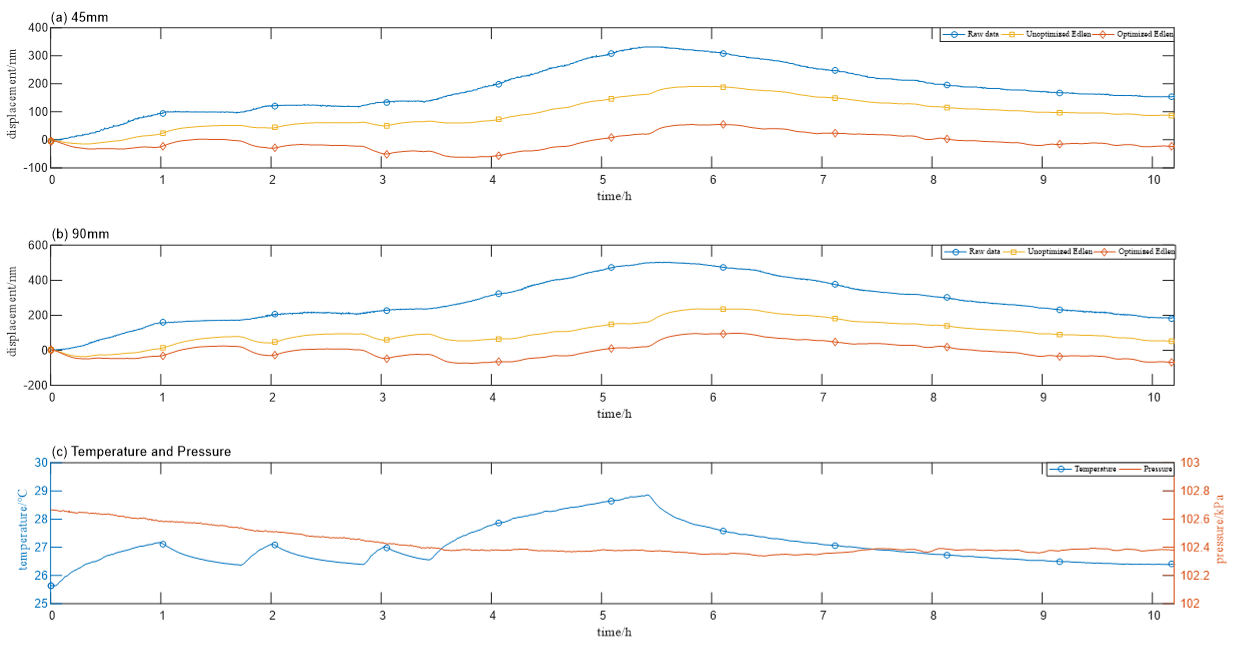
\includegraphics[width=14cm]{fig/4-fig/温度梯度实验数据.jpg}
  \caption{温度梯度实验数据}
  \label{fig:温度梯度实验数据}
\end{figure}

测量时间约为$10.2h$,温度变化范围为$[25.64\,\,\,28.85]^{\circ}C$,气压变化范围为$[102.7\,\,\,102.4]kPa$,测量臂长度为$45nm$和$90nm$的两套干涉仪的原始位移数据的变化范围为$[0 \,\,\, 301.3]nm$和$[0\,\,\,582.4]nm$,在考虑可能含有随机误差等其他误差的情况下,可近似认为两者成两倍关系。并且对于零位测量而言,上述位移变化都可以认为是误差,对应的均方根误差分别为$201.8186nm$和$379.4892nm$。经过Edlen公式补偿后的均方根误差为$108.9044nm$和$124.7847nm$,补偿效果约为$46\%$和$67\%$。使用粒子群算法进行优化之后再进行补偿,测量臂长度为$45nm$的干涉仪的残留均方根误差从$108.9044nm$降低为$30.4053 nm$,而$90nm$长度的则从$124.7847nm$降低为$45.8778nm$,两者残差的差值仍有$15.4725nm$,相较于未优化前的差值$15.8803nm$几乎没有提升,这说明这说明环境误差的补偿效果得到一定改善,但补偿的精准性却不一定有提升。

从图中可以看出,$1\sim2h$、$2\sim3h$时间内,温度在$26^{\circ}C\sim27^{\circ}C$范围内来回变化,在$3.4\sim10h$内,温度则从$26^{\circ}C$上升到$28.85^{\circ}C$,随后又回到$26^{\circ}C$,前两次的温度梯度明显大于最后一次的温度梯度。从补偿结果也可以看出,红色曲线为经过粒子群算法优化后的Edlen公式的补偿效果,相较于原始Edlen公式的补偿效果(黄色曲线),红色曲线明显更加贴近理论位移值0nm。但黄色曲线以及红色曲线在上述三个温度波动范围也有明显波动,并且第三个温度波动范围内对应的补偿结果波动较前面两个显得更加平缓,与温度梯度值的大小相对应。这进一步说明了,在大温度梯度的情况下,可能引入了其他误差因素,导致线性形式的Edlen公式无法适用。

\section{基于温度梯度的分段式粒子群算法补偿方法}
\label{温度梯度的分段式粒子群算法补偿方法}
\subsection{算法原理}
由前文所述可知,在大温度梯度的情况下,可能引入了其他误差因素(例如大气湍流),导致线性形式的Edlen公式无法适用,此时的补偿模型可能是非线性的。但是由微积分的思想可知,一个非线性的函数只要微分的粒度足够小,在每一个$\Delta t$区间内都可以看做是线性的。所以只需要进行分段,然后在各个微分段内,Edlen公式仍是可以使用的。由于温度梯度才是导致上述问题的原因,那么在进行分段补偿的时候,自然使用温度梯度作为分段的依据,在本文所述的工作中,采用如下两种分段的方法:
\begin{enumerate}
  \item 采用单组温度传感器,使用自身温度的变化梯度作为分组依据,即在一定的时间内,温度的变化超过某个定值就进行一次分段。
  \item 采用两组温度传感器,两组传感器放置的位置具有一定距离,采用同时刻两个传感器的差值作为分组依据,即在同一时刻,两个传感器的差值大于某个定值就进行一次分段。
\end{enumerate}

值得说明的是,在本文进行的实验中,上述两种分段方法的补偿效果差别不大(不超过$3.5\%$),但是第一种方法操作较为简便,所以建议使用第一种方法,本文后续的工作使用的也是第一种方法,使用的阈值为:80个数据点内,温度的变化超过$0.05^{\circ}C$

\subsection{算法流程图}
\label{基于温度梯度的分段式粒子群算法补偿流程图}
算法的流程图如图\ref{fig:基于温度梯度的分段式粒子群算法补偿流程图}所示。
\begin{figure}[htb]
  \centering
  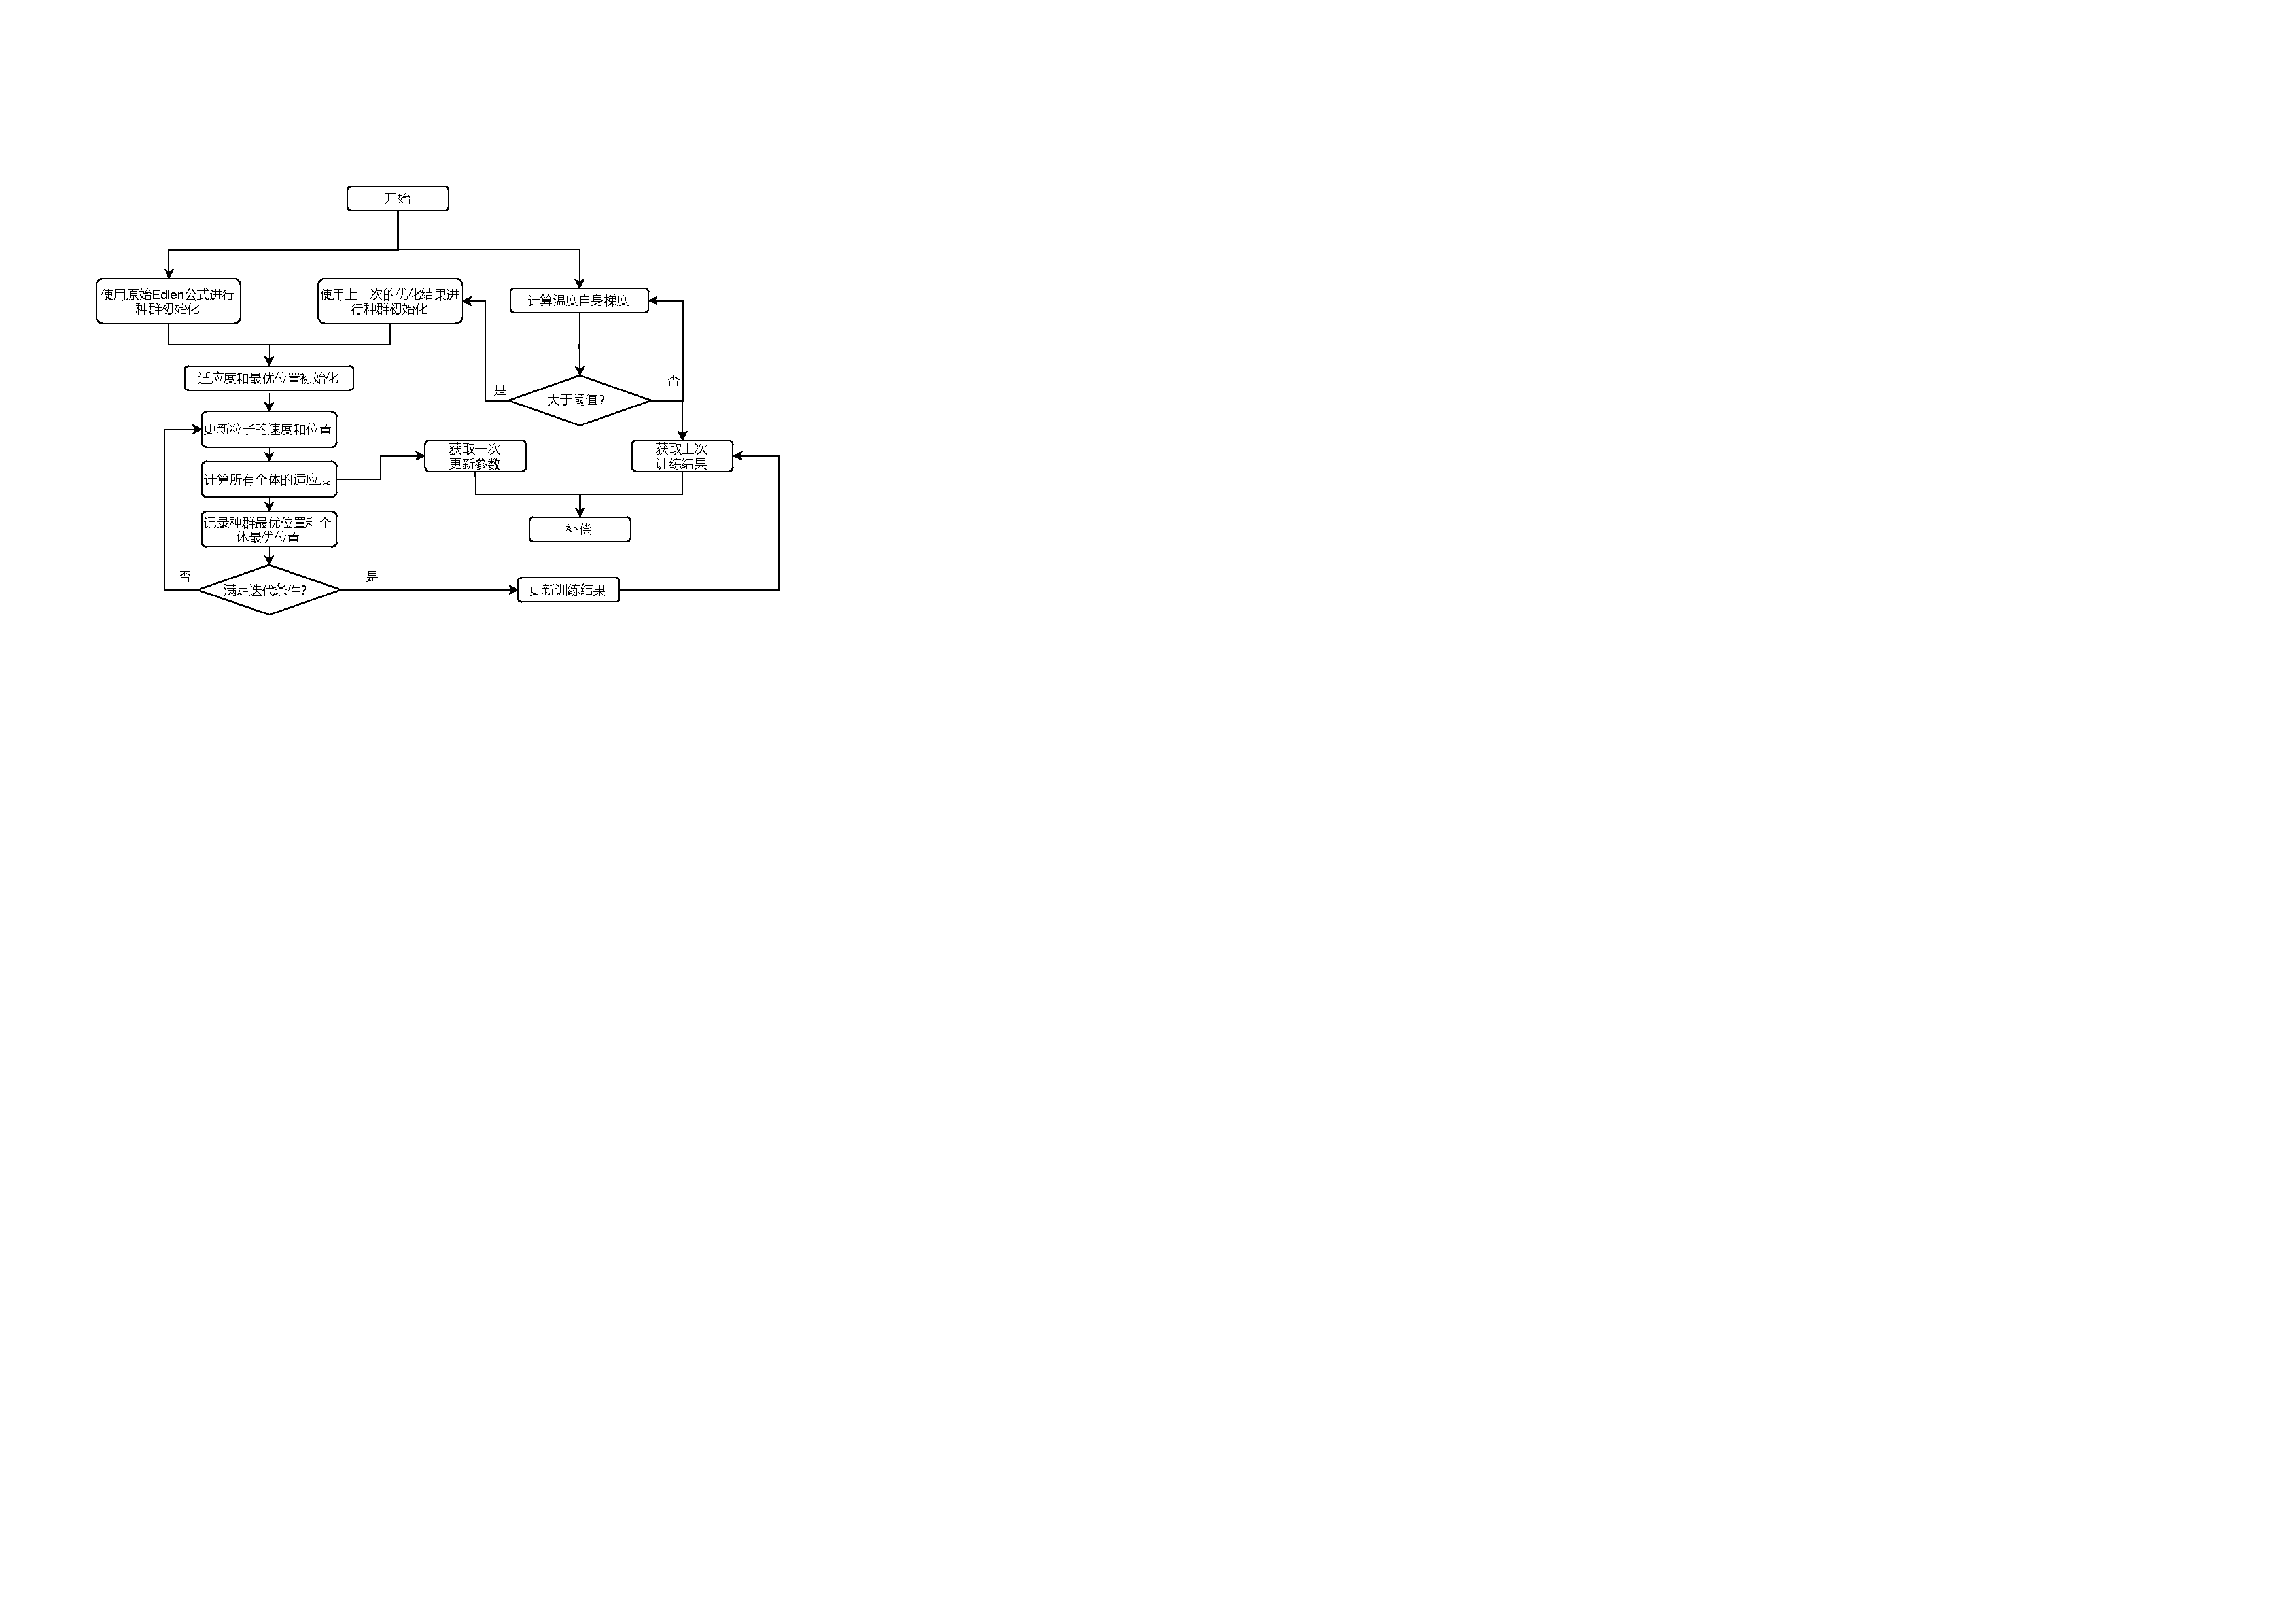
\includegraphics[width=12cm]{fig/4-fig/基于温度梯度的分段式粒子群算法流程图.drawio.pdf}
  \caption{基于温度梯度的分段式粒子群算法补偿流程图}
  \label{fig:基于温度梯度的分段式粒子群算法补偿流程图}
\end{figure}

跟之前介绍的整段式粒子群算法补偿方法不同,当由于温度变化梯度过大导致触发分段进行新的一次粒子群算法训练时,种群的初始不再是设置为原始的Edlen公式,而是设置为触发分段之前的粒子群算法的训练结果,这就意味着在进行新的一次分段训练的前期,进行补偿的Edlen公式模型并不是粒子群算法训练出来的最优解,而是一个更上一次训练结果比较接近的次优解,这么做是为了让补偿结果的曲线比较平滑,防止在两次分段训练的交界处,由于补偿模型的突然改变而使得补偿结果曲线出现突然的断落。但由于使用了一个次优解而非最优解,势必会对补偿精度造成一定损失,损失的大小取决于采样周期与粒子群算法计算速度之间的关系。采样周期越长,粒子群算法计算速度越快,那么在进行新的一次分段补偿时,能够给粒子群算法训练的时间也就越多,训练效果也就越好,精度损失也就越小,反之亦然。由于温度梯度改变可能会导致触发新的一次分段训练,但当前训练的迭代次数可能还没达到设置的迭代上限就开始了新的一轮训练,从而使得上轮训练不彻底。所以迭代条件不能简单用迭代次数进行控制,为此增加了使用适应度大小进行控制,即迭代次数到达上限或者适应度小于设定的阈值,视为完成一轮迭代。

\subsection{补偿效果}
实验数据如图\ref{fig:基于温度梯度的分段粒子群算法补偿效果}所示。(a)图为测量臂长度为$45nm$的位移测量数据,(b)图为测量臂长度为$90nm$的位移测量数据,(c)图为对应的温度和气压数据,(a)、(b)、(c)三图的横轴均为时间,单位为h;(a)和(b)图中的竖轴为位移数据,单位为$nm$,其中带圆圈标注的蓝色曲线为原始的位移测量数据,带黄色方块标注的为使用原始Edlen公式补偿后的位移数据,带红色菱形标注的为使用粒子群算法优化后的补偿后位移数据,带五角星形标注的则为基于温度梯度的分段粒子群算法补偿后的位移数据;(c)图的竖轴为温度和气压数据,单位为$^{\circ}C$和$kPa$,其中带圆圈标注的蓝色曲线为温度数据,红色曲线为气压数据。

\begin{figure}[htb]
  \centering
  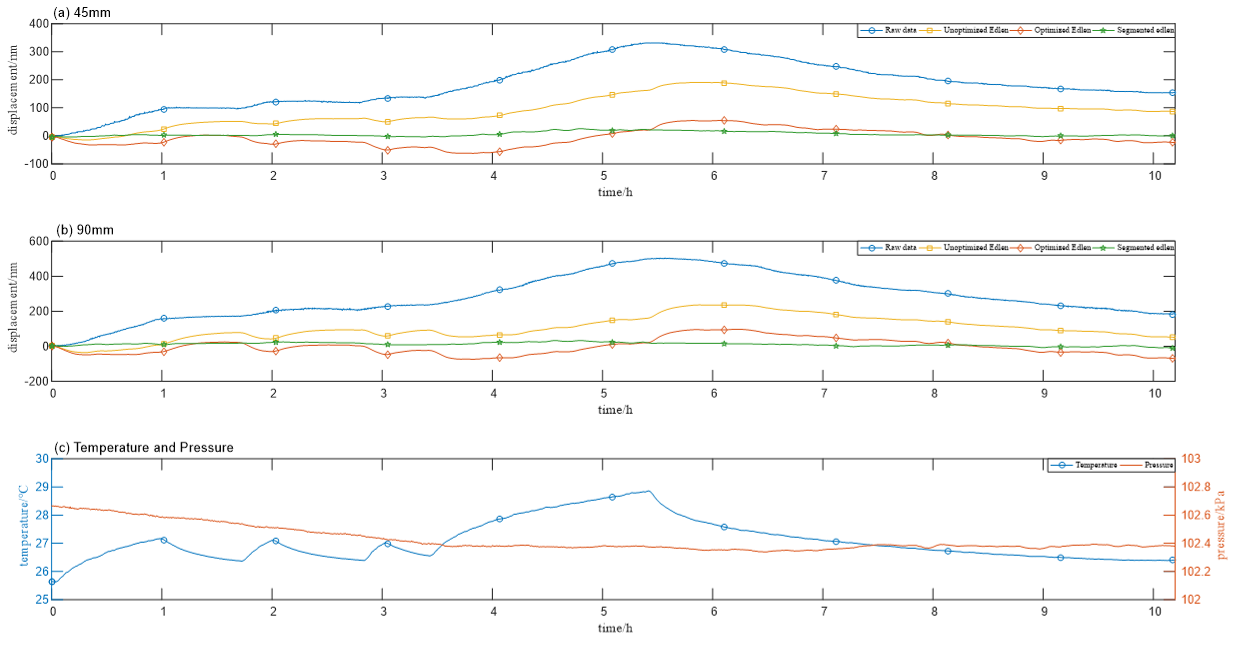
\includegraphics[width=14cm]{fig/4-fig/基于温度梯度的分段粒子群算法补偿效果.jpg}
  \caption{基于温度梯度的分段粒子群算法补偿效果}
  \label{fig:基于温度梯度的分段粒子群算法补偿效果}
\end{figure}

数据上,相比经过整段式粒子群算法的补偿效果,在经过E温度梯度的分段粒子群算法补偿后的均方根误差从$30.4053 nm$降低到了$10.7903 nm$($45nm$)、从$45.8778 nm$降低到了$13.1134 nm$($90nm$),剩余的残差也仅仅只有$2.3631nm$,这个数值甚至小于干涉仪的分辨率,所以完全可以认为补偿后的残差是相等的,即可以说明环境误差得到了比较精确且完全的补偿。图形上也可以看出,绿色的线几乎全程保持一条直线,并没有过大的波动。

\subsection{不足之处}
需要特别指出的是,基于温度梯度的分段式粒子群算法补偿方法仍然有着以下几个不足之处:
\begin{enumerate}
  \item 进行分段时所使用的依据:80个数据点内,温度的变化超过$0.05^{\circ}C$也是一个经验值,是根据本文工作的实验数据分析出的一个补偿效果比较理想的值,这就意味着也可能存在上文所述的诸如温度不匹配或其他类似问题,这可能也会一定程度上影响补偿效果。
  \item 如\ref{section:实验环境改进}节所述,本文的所有工作都未在亚克力罩中设置任何的直接热源,温度梯度的值无法做到太大,这就导致了未验证过当温度梯度进一步增大时,基于温度梯度的分段式粒子群算法补偿方法的效果如何。
  \item 如\ref{基于温度梯度的分段式粒子群算法补偿流程图}节所述,采样周期越长,粒子群算法计算速度越快,两者之间的差值越大,那么在每次分段补偿的初期补偿效果损失越小。但是当前干涉仪的应用场合下,大多无法做到过低的采样频率,所以需要想办法增加粒子群算法计算速度。
  \item 如\ref{基于温度梯度的分段式粒子群算法补偿流程图}节所述,可能会出现当前训练的迭代次数可能还没达到设置的迭代上限就开始了新的一轮训练的情况,虽然使用适应度控制迭代条件能减少该情况的发生,但是适应度阈值的取值也有着一定的要求,适应度阈值过大则仍旧可能会发生上述现象。一般的,在同样的时间内,粒子群算法计算的越快,则迭代计算的结果更优,即适应度更小,需要想办法增加粒子群算法计算速度。
  \item 由于进行了多次分段,这使得整个补偿程序的计算量是明显大于整段式粒子群算法补偿方法的,处于补偿及时性的考虑,计算量增大了需要增加计算速度才能动态平衡。
\end{enumerate}

前两点算是本文工作真正存在的局限性,而后三点的解决办法都相同:提高粒子群算法的计算速度。粒子群算法本质上是一个迭代计算和并行计算相互组合的过程,在达到迭代条件之前需要一直迭代,并且每次迭代需要并行计算每个个体的适应度、更新种群信息、更新个体速度和位置等,其本身计算量就不小。而温度梯度的分段式粒子群算法补偿方法,由于根据温度变化梯度进行分段训练和补偿,将粒子群算法的这一缺点进行了放大。而在当前处理器性能,专用处理器是大于通用处理器的,而粒子群这样一个含有大量并行计算的算法,提升其计算速度的一个有效方法就是设计粒子群算法的专用处理器。

\section{算法硬化}
软件层面和硬件层面的设计是不相同的,软件注重简洁性、高效性,而硬件注重的是面积、功耗、性能三者之前的权衡,所以通常在做硬件实现的时候,都需要对算法做一定更改,使其更加符合硬件设计的逻辑,这步称为算法硬化。硬化后的算法也可以在最后的RTL(Register Transfer Level,寄存器传输级)的参考模型,称为RTL model。

\subsection{数据定点方案及截断方案}
由于在硬件的视角中,只能识别两个电平:0和1,对应的即为二进制数,并且硬件是无法自动识别小数的,当前硬件中表示小数的方案有两种:定点和浮点。定点数指的是约定所有数据都有着一个隐含的小数点,并且这个小数点位置是固定的,例如8bit的数据(bit7-bit0),bit4和bit3之间为小数点位置,那么高4bit数据(bit7-bit4)则表示整数部分,低4bit数据(bit3-bit0)则表示小数部分,如果是一个有符号数,那么往往在最高位增加1bit(bit8)用来表示正负,如图\ref{fig:定点数示意图}所示,其中1表示负数,0表示正数,例如一个9bit数9'h001011010,由于bit8为0,所以这是一个正数,而bit7-bit4为4'b0101,对应的十进制数为3,所以整数部分为3,而bit3-bit0为4'b1010,对应的十进制数为10,由于这是小数部分,而且是4bit的小数,所以对应的小数精度为$\frac{1}{2^4}$,所以小数部分对应的十进制数为$3+10\times\frac{1}{2^4}=3.625$。浮点数则是指小数点的位置是不固定的,用尾数和阶码表示一个浮点数,其中尾数决定了浮点数的精度并决定了数字的正负,阶码则决定了小数点在数据中的实际位置,科学计数法就是一种常见的浮点数表示方法,例如一个科学计数法表示的数$1.3564\times10^{2}$,其中1.3564则为尾数,它决定了这个数字的精度为0.01;2则为阶码,它决定了小数点的实际位置是在5之后。
\begin{figure}[htb]
  \centering
  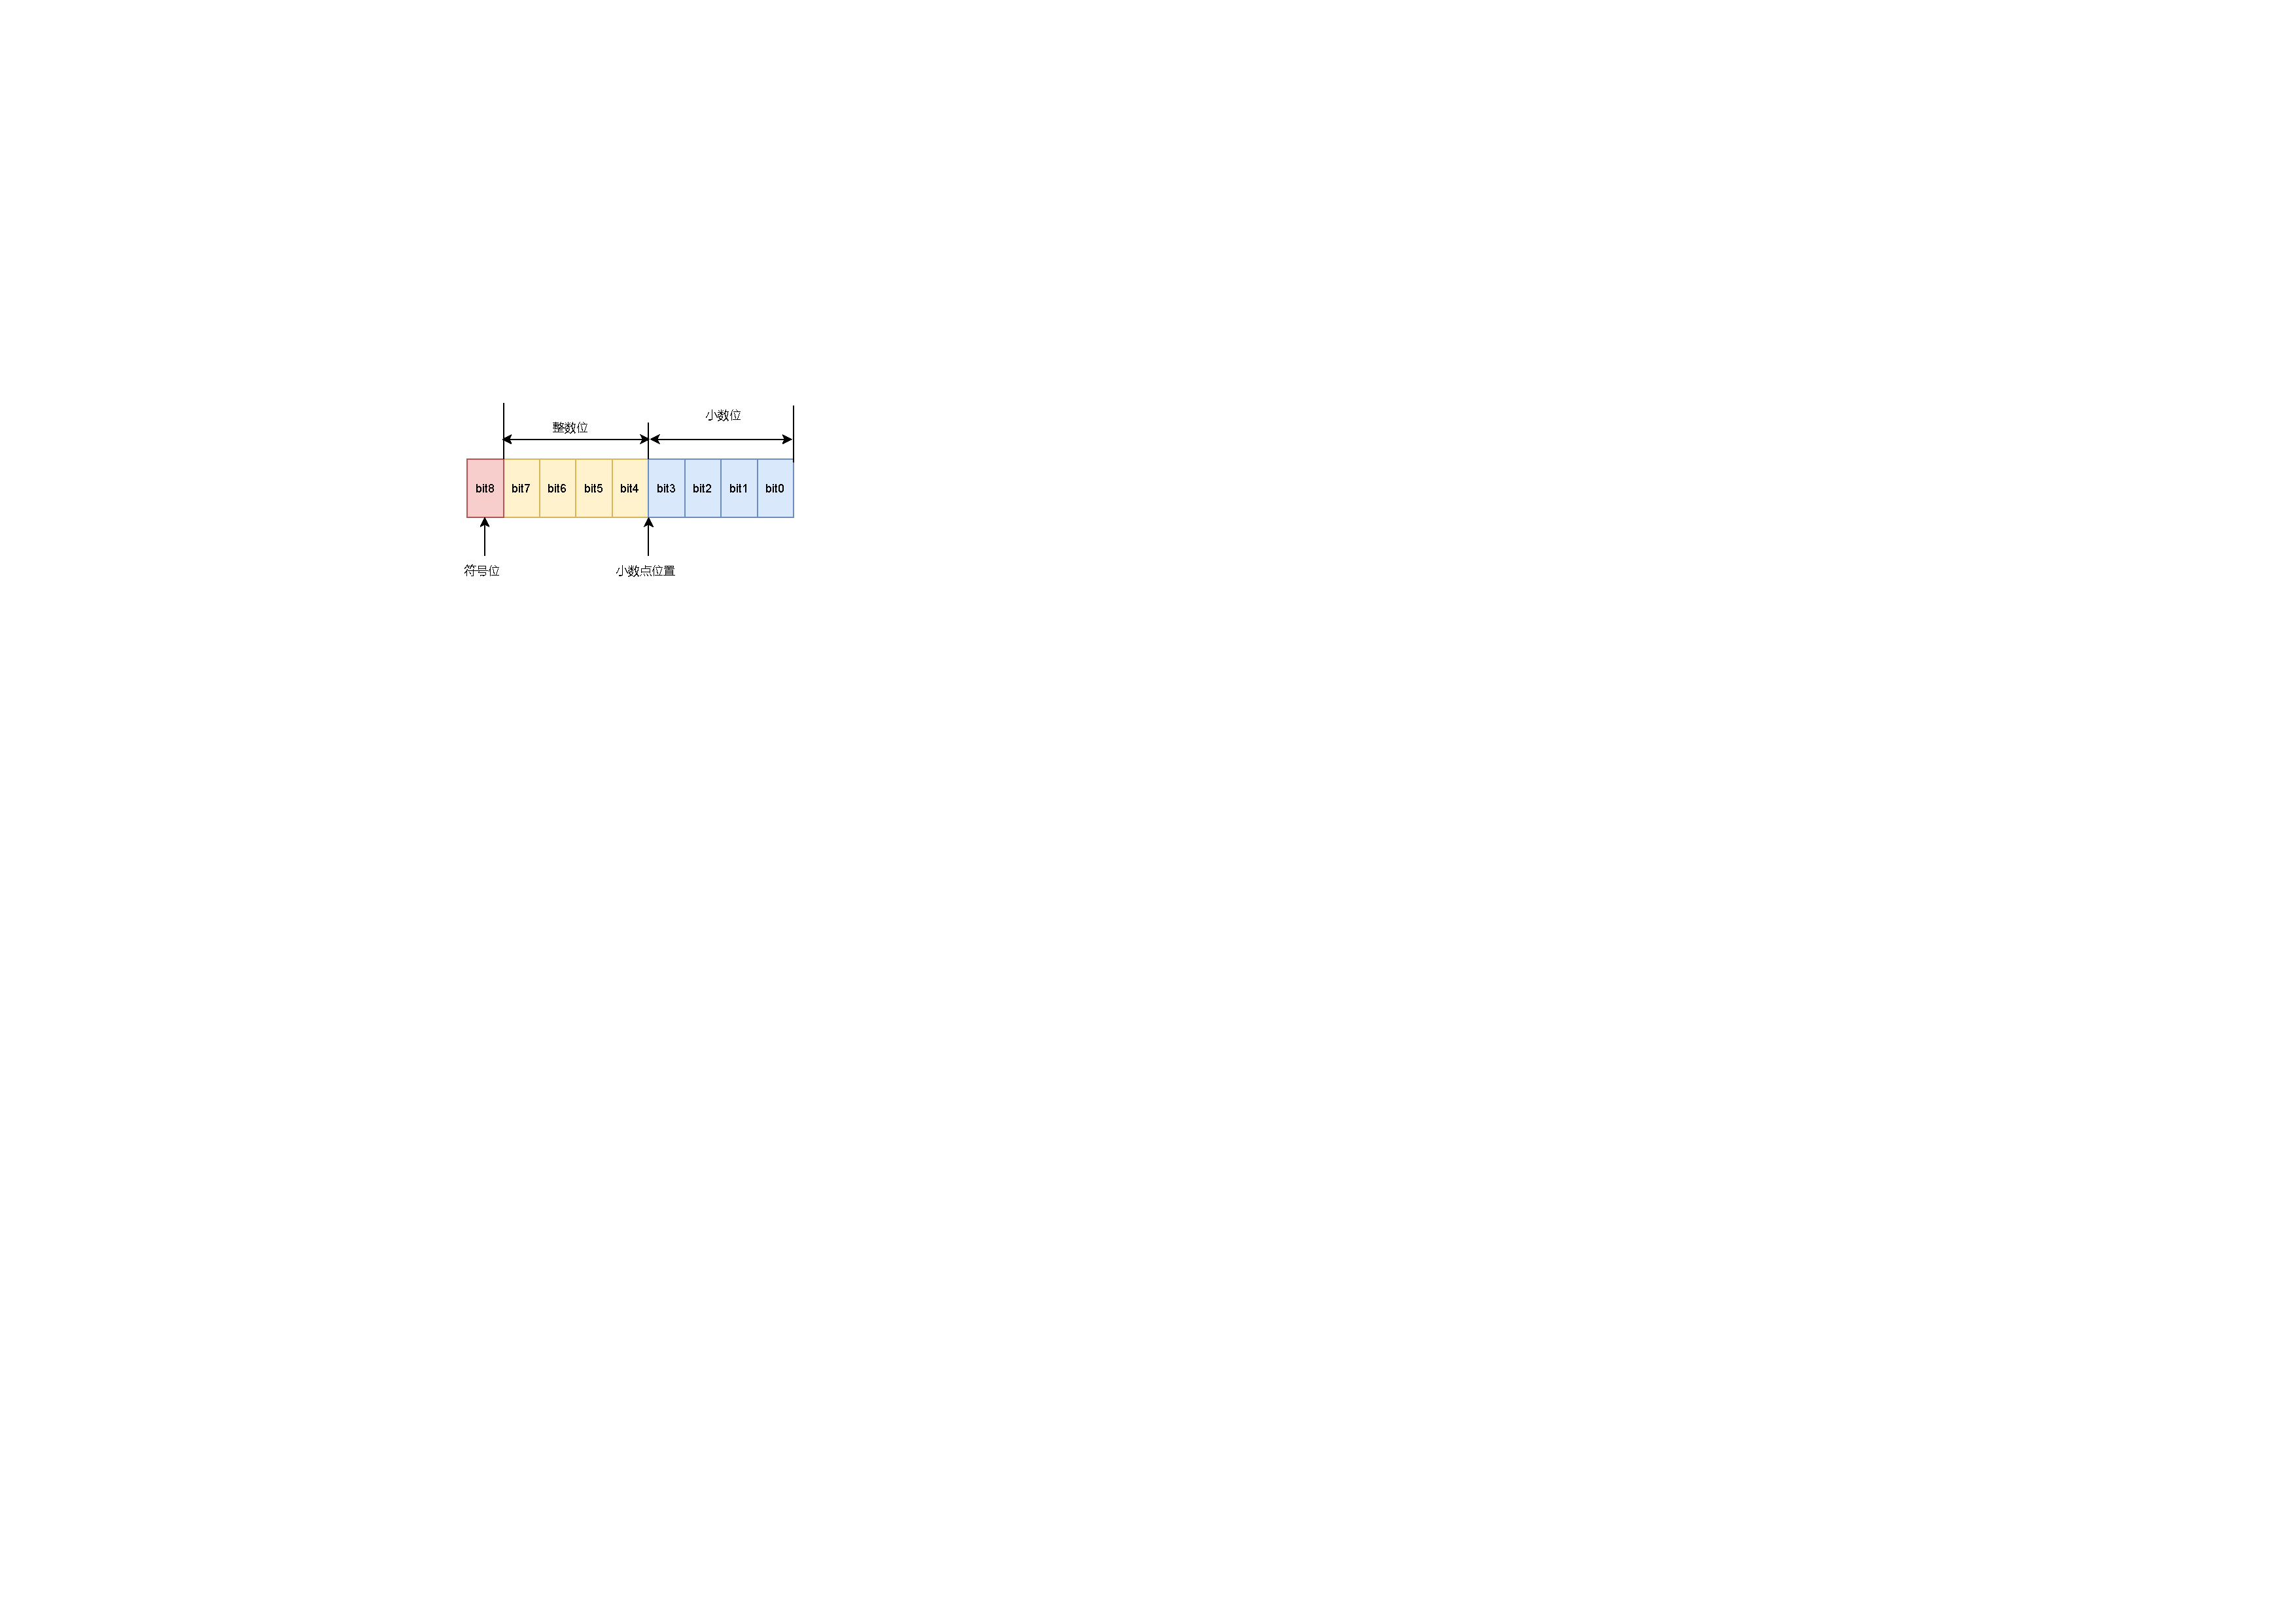
\includegraphics[width=9cm]{fig/4-fig/定点数示意图.drawio.pdf}
  \caption{定点数示意图}
  \label{fig:定点数示意图}
\end{figure}

定点数与浮点数相比,由于小数点的位置是固定的,所以能表示的数值范围也是固定且小于浮点数的表示范围的,这导致可能会存在数值溢出的问题,但是定点数有着一个最大的优点:定点数对应的计算单元运算更快,并且消耗更少的资源和功率,所以为了提高粒子群算法的计算速度,定点数是比浮点数更好的选择。

所以本文采用1bit符号位加上15bit整数加上8bit小数共24bit的定点方案,小数部分最大截断误差约为0.0039,该方案能够表示的数据范围约为$-32768nm\sim32767nm$,如果需要表示超过上述范围的数字,需要增加整数部分的比特位宽,想增加数字精度则需要增加小数部分的比特位宽,但这都会带来硬件资源的增加以及性能的下降。

需要注意的是,由于采用了定点方案使得能表示的数值精度是一定的,但是硬件计算加法和乘法的时候,计算结果的比特位宽是会变化,有如下规律:加法结果的数值比特位宽为两个加数之中最大的数值比特位宽+1,乘法结果的数值比特位宽为两个乘数的数值比特位宽之和(注意是数值比特位宽,符号位另作计算),而比特位宽的改变可能会使得在如上所述的24bit定点方案中的精度发生改变,这是错误的,所以实时进行截断。例如两个24bit的定点数相乘,其数值的比特位宽是23bit加1bit的符号位,所以其计算结果是46bit加上1bit的符号位,共计47bit,但是这其中包含了30bit的整数部分和16bit的小数部分,而定点数的精度是一定的,为8bit,经过乘法计算后却增大到了16bit,所以需要将计算结果的最低8bit进行截断。一旦进行了截断就势必会引入误差,而且不同的截断方案引入的误差会是不一样,例如计算$A\times B+C$(A、B、C)均为24bit的定点数,有两种截断方案:计算完$A\times B$后截断和$A\times B+C$全部计算完之后再截断,前者由于计算中途就进行了截断,从而损失了8bit的精度,这会导致误差的累计,但由于少了8bit数,所以可以减少硬件资源的消耗,所以有利有弊。本文综合使用两种截断方案,在需要较高精度的场合,例如适应度计算,采用第二种截断方案以提高计算精度,从而能够比较出适应度非常接近的两个粒子究竟谁更优,而在其余场合则使用第一种截断方案,从而达到节省硬件资源开销的目的。

\subsection{补码运算}
24bit的定点数方案共定义了1bit符号位以及23bit的数值位,对于这样的有符号数,硬件需要区分数据的符号位以及数值位,并且减法器的设计是比加法器更加复杂的,需要更多的硬件资源,所以使用补码将符号位和数值位、加法和减法相统一,这样做能简化硬件层面的设计。

在介绍补码之前需要先简单介绍补码和反码,原码就是指的有符号二进制数本身,而正数的反码也等于它本身,负数的反码则等于其原码除符号位外所有比特位都取反,补码则等于其反码加上1。对于正数而言,原码、反码、补码完全一致,所以实际上原码、反码和补码只对负数具有实际的应用意义。\ref{fig:补码计算示意图}给出了一个8bit有符号数(十进制为-53)的补码计过程。
\begin{figure}[htb]
  \centering
  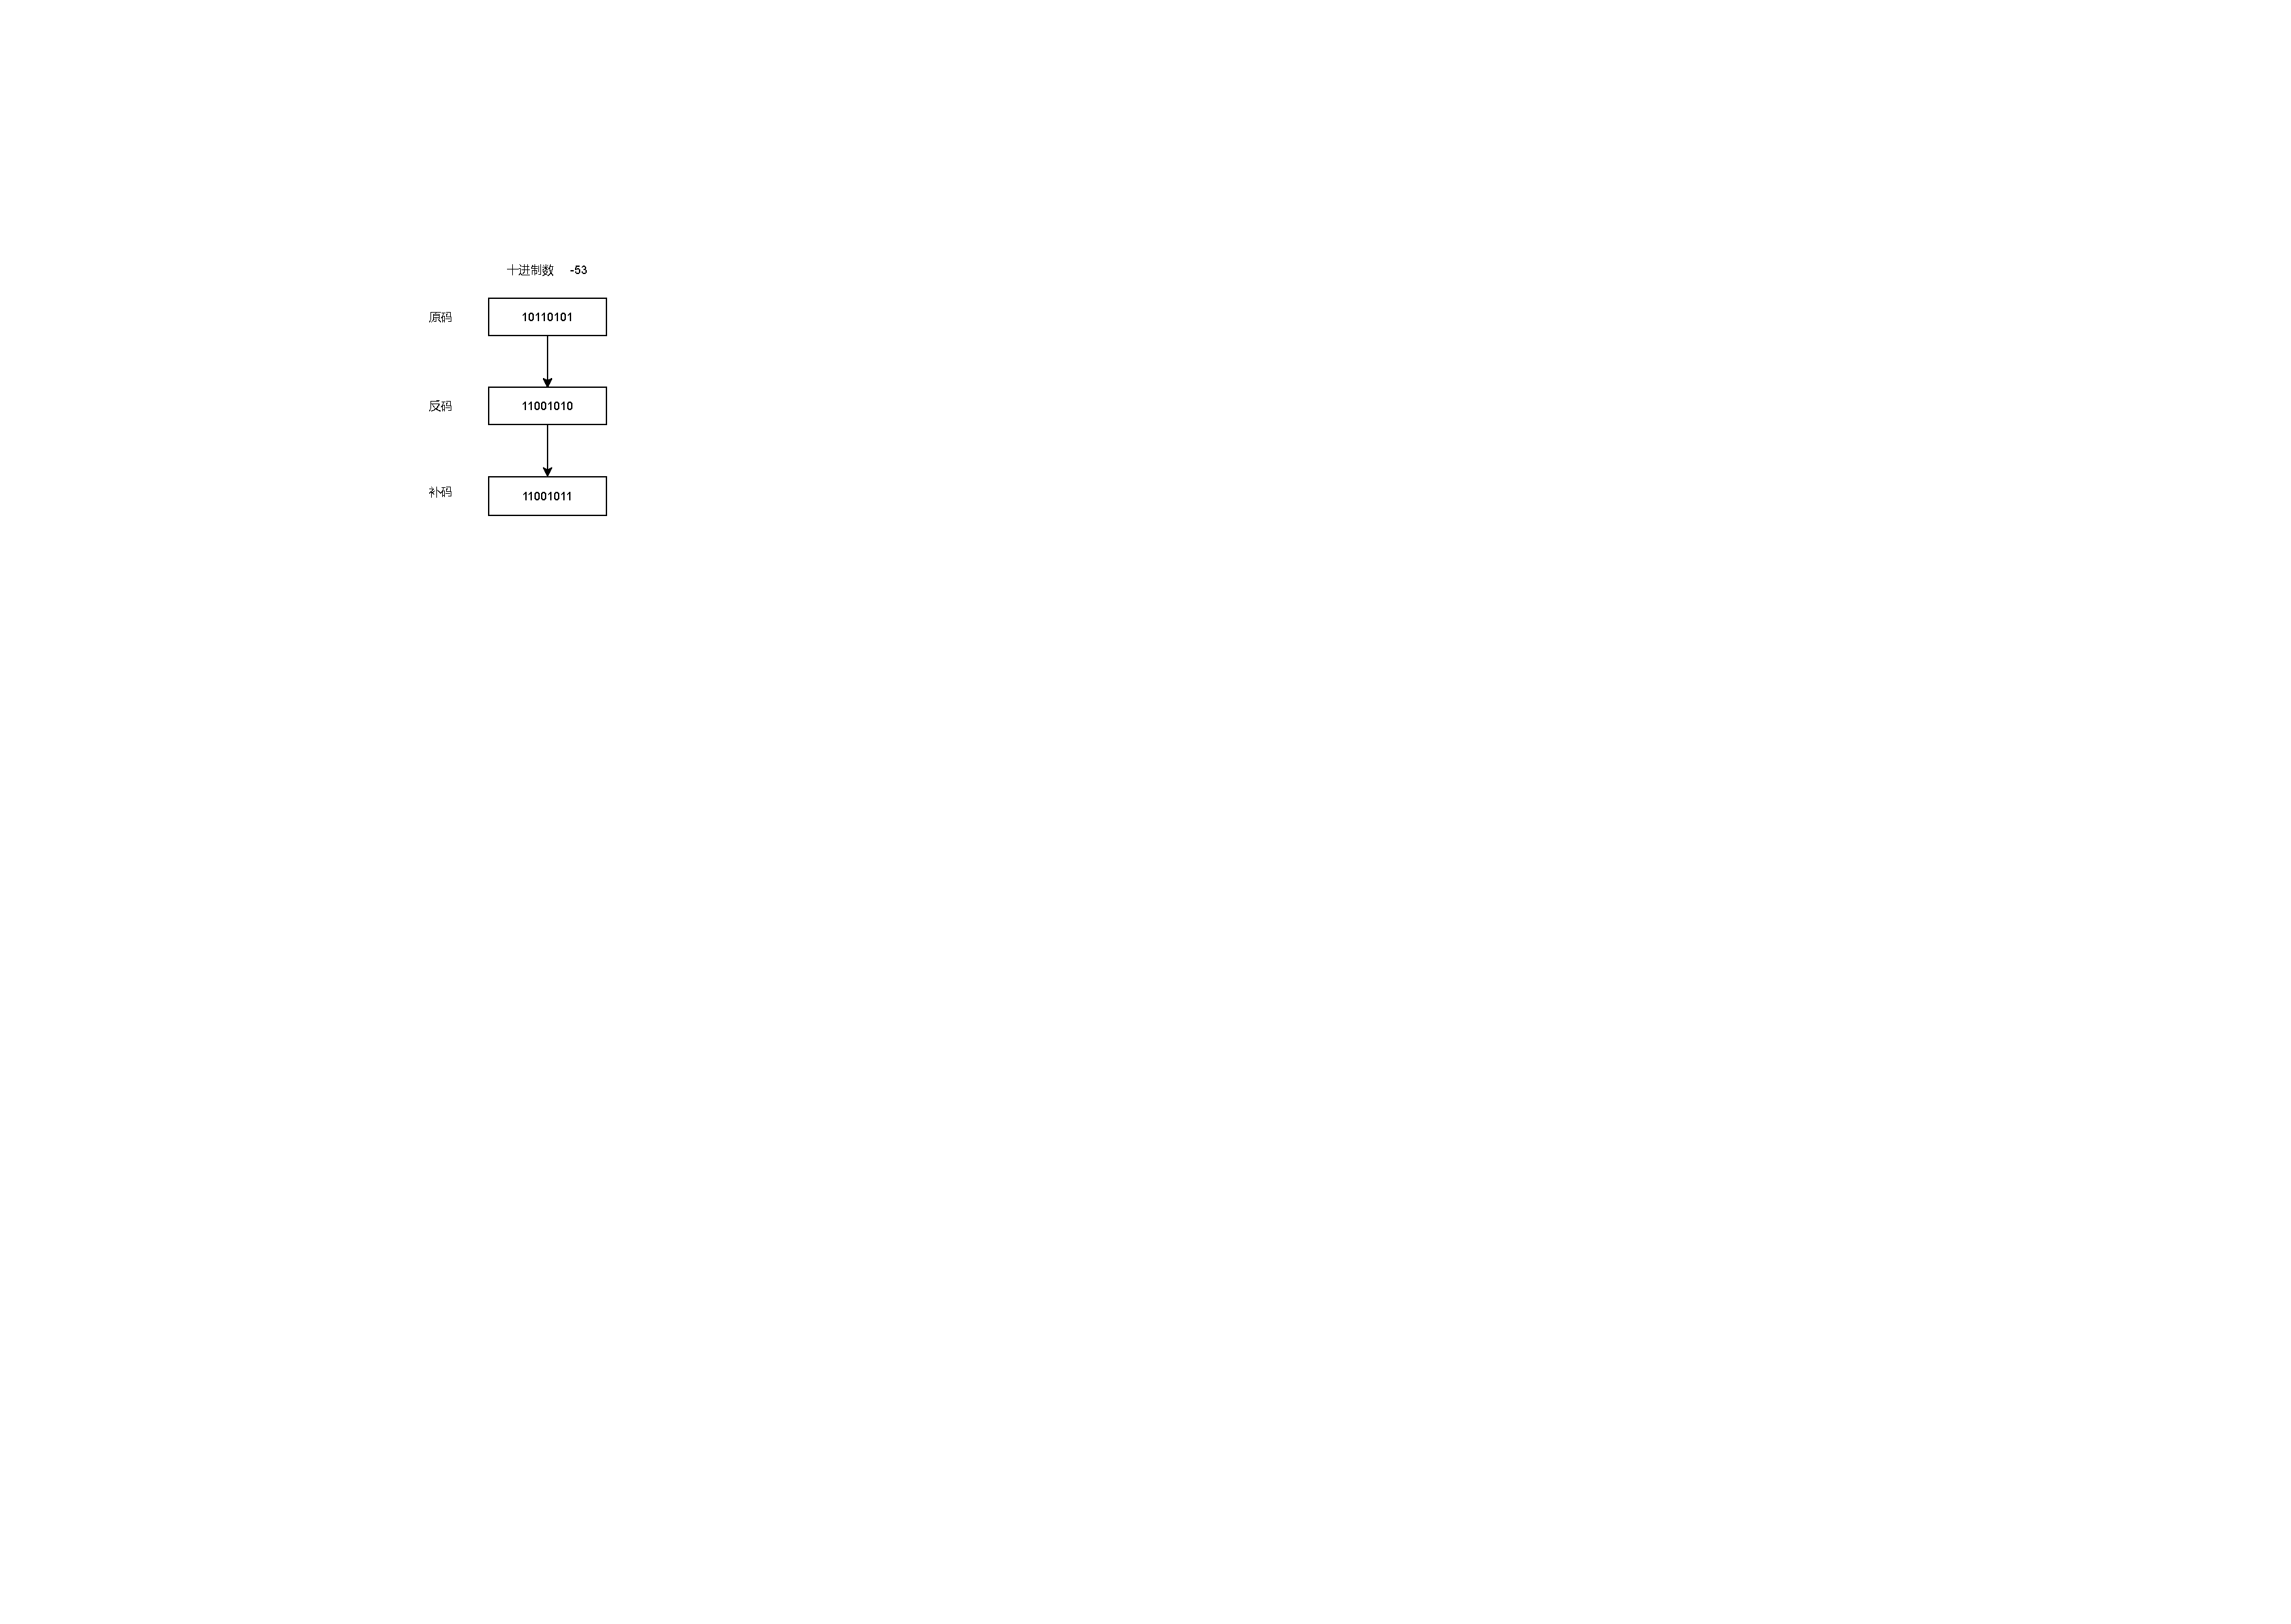
\includegraphics[width=7cm]{fig/4-fig/补码计算示意图.pdf}
  \caption{补码计算示意图}
  \label{fig:补码计算示意图}
\end{figure}

\subsection{乘除转换转换}
在硬件的世界中,四则运算所需要的资源量关系为:除法>乘法>加(减)法,导致性能下降的程度关系为:除法>乘法>加(减)法,但是其中有一个特殊情形,即2次幂乘法或除法,由于二进制数第nbit表示的十进制数大小为$2^{n-1}$,这说明距离为l的两个bit位其对应的倍数关系为$2^{l}$,所以如果是2的n次幂的乘法或除法,只需要将二进制数左移(对应乘法)或者右移(对应除法)nbit即可,移位操作在硬件中是非常容易实现的,所以这并不会使用大量的硬件资源或者降低性能。而对于非2的n次幂的乘法或除法,可以转换为多个2的幂次方乘加,然后转换为移位操作。例如$A\times 19$可以转换为$A\times 16 +A\times 2+A$,之后就可以使用移位操作替换乘法。但除了上述特殊情况,其余情况在硬件设计的时候需要尽可能避免除法的使用,并且减少乘法的使用。

由于在粒子群算法的适应度计算时采用的是均方根误差,而均方根误差的计算公式如式\eqref{eq:均方根误差计算公式}所示,是需要进行一次除N的操作的,这个N取决于粒子群算法设置的种群个体数。由前文所述,如果这个N是2的幂乘法,那么就可以将除法的操作转变为移位操作,所以本文推荐粒子群算法的种群个体数设置为16、32、64、128,这样在计算均方根误差时只需要将数据右移4、5、6、7位即可。

\subsection{四舍五入方案}
软件层面进行四舍五入非常简单,只需要判断是否小于阈值即可,放在硬件层面,判断数值是否小于阈值对应的基本逻辑单元是比较器,常见的基本逻辑单元面积关系为:加法器>比较器>选择器,比较器的面积不大不小,所以如果能减少比较器的使用数量,也能在资源消耗上带来一定收益。

所以本文进行四舍五入时采用如下方案:假设是在判断小数部分是否需要四舍五入时,即判断低8bit是否需要像第9bit进位时,可以将数值加上8'b10000000,然后右移8位即可。这么做的原理是如果需要判断低8bit是否需要四舍五入,其实只需要判断第8bit的值是否为1,如果为1,那么这个数值是一定大于8bit数最大值(255)的一半的,这时就需要进位,然后进行移位即可舍去由于加法而导致的多余数据;如果第8bit为0,那么即使加上8'b10000000也不会产生进位,进行移位后即可以完成舍入过程。而加上一个2的幂次方是可以通过异或门实现,这样做就可以减少资源消耗了。

\section{硬化前后的算法验证框架}
\subsection{进制转换与字符串操作}
由于补偿算法使用matlab编写,并且对应的硬化后的算法参考模型也是使用matlab编写的,而matlab本身对二进制计算并不友好,所以模型验证时采用了多次进制转换与字符串操作,这些操作使用matlab自带的dec2hex、hex2dec、bin2dec、num2str等函数。

\subsection{RTL model验证框架}
\label{RTL model验证框架}
RTL model的验证框架示意图如图\ref{fig:RTL model验证框架}所示,三角箭头表示数据类型为数值,蓝色线条代表进制为十六进制,绿色线条代表进制为二进制,黑色线条代表该处为其他类型操作(比较、控制等)。验证框架主要由4部分组成:stimulator、RTL model、software、scoreboard。其中stimulator主要功能为产生测试激励,主要包含driver和monitor两个部件,monitor进行激励产生的控制,driver产生受控的测试激励。RTL model为硬化后的粒子群算法,包含三个部件:fitnesee$\_$cal(进行适应度的计算)、population$\_$upda(进行种群信息的更新)、velocity$\_$upda(进行速度和位置的更新),三者的输出都是十六进制类型的数值,输入都是二进制类型的数值,所以在上一级模块输出和下一级模块输入之间需要进行进制的转换,但在三个模块内部计算时所有数据都为十进制。software软件版本的粒子群算法,即上文中用于实验中的补偿程序,RTL model中每一部分在software中都有对应部分,作为验证RTL model正确性时的参考模型。scoreboard为得分板,比较RTL model和software的输出是否一致,并在误差大小超出设定阈值是进行报错。
\begin{figure}[htb]
  \centering
  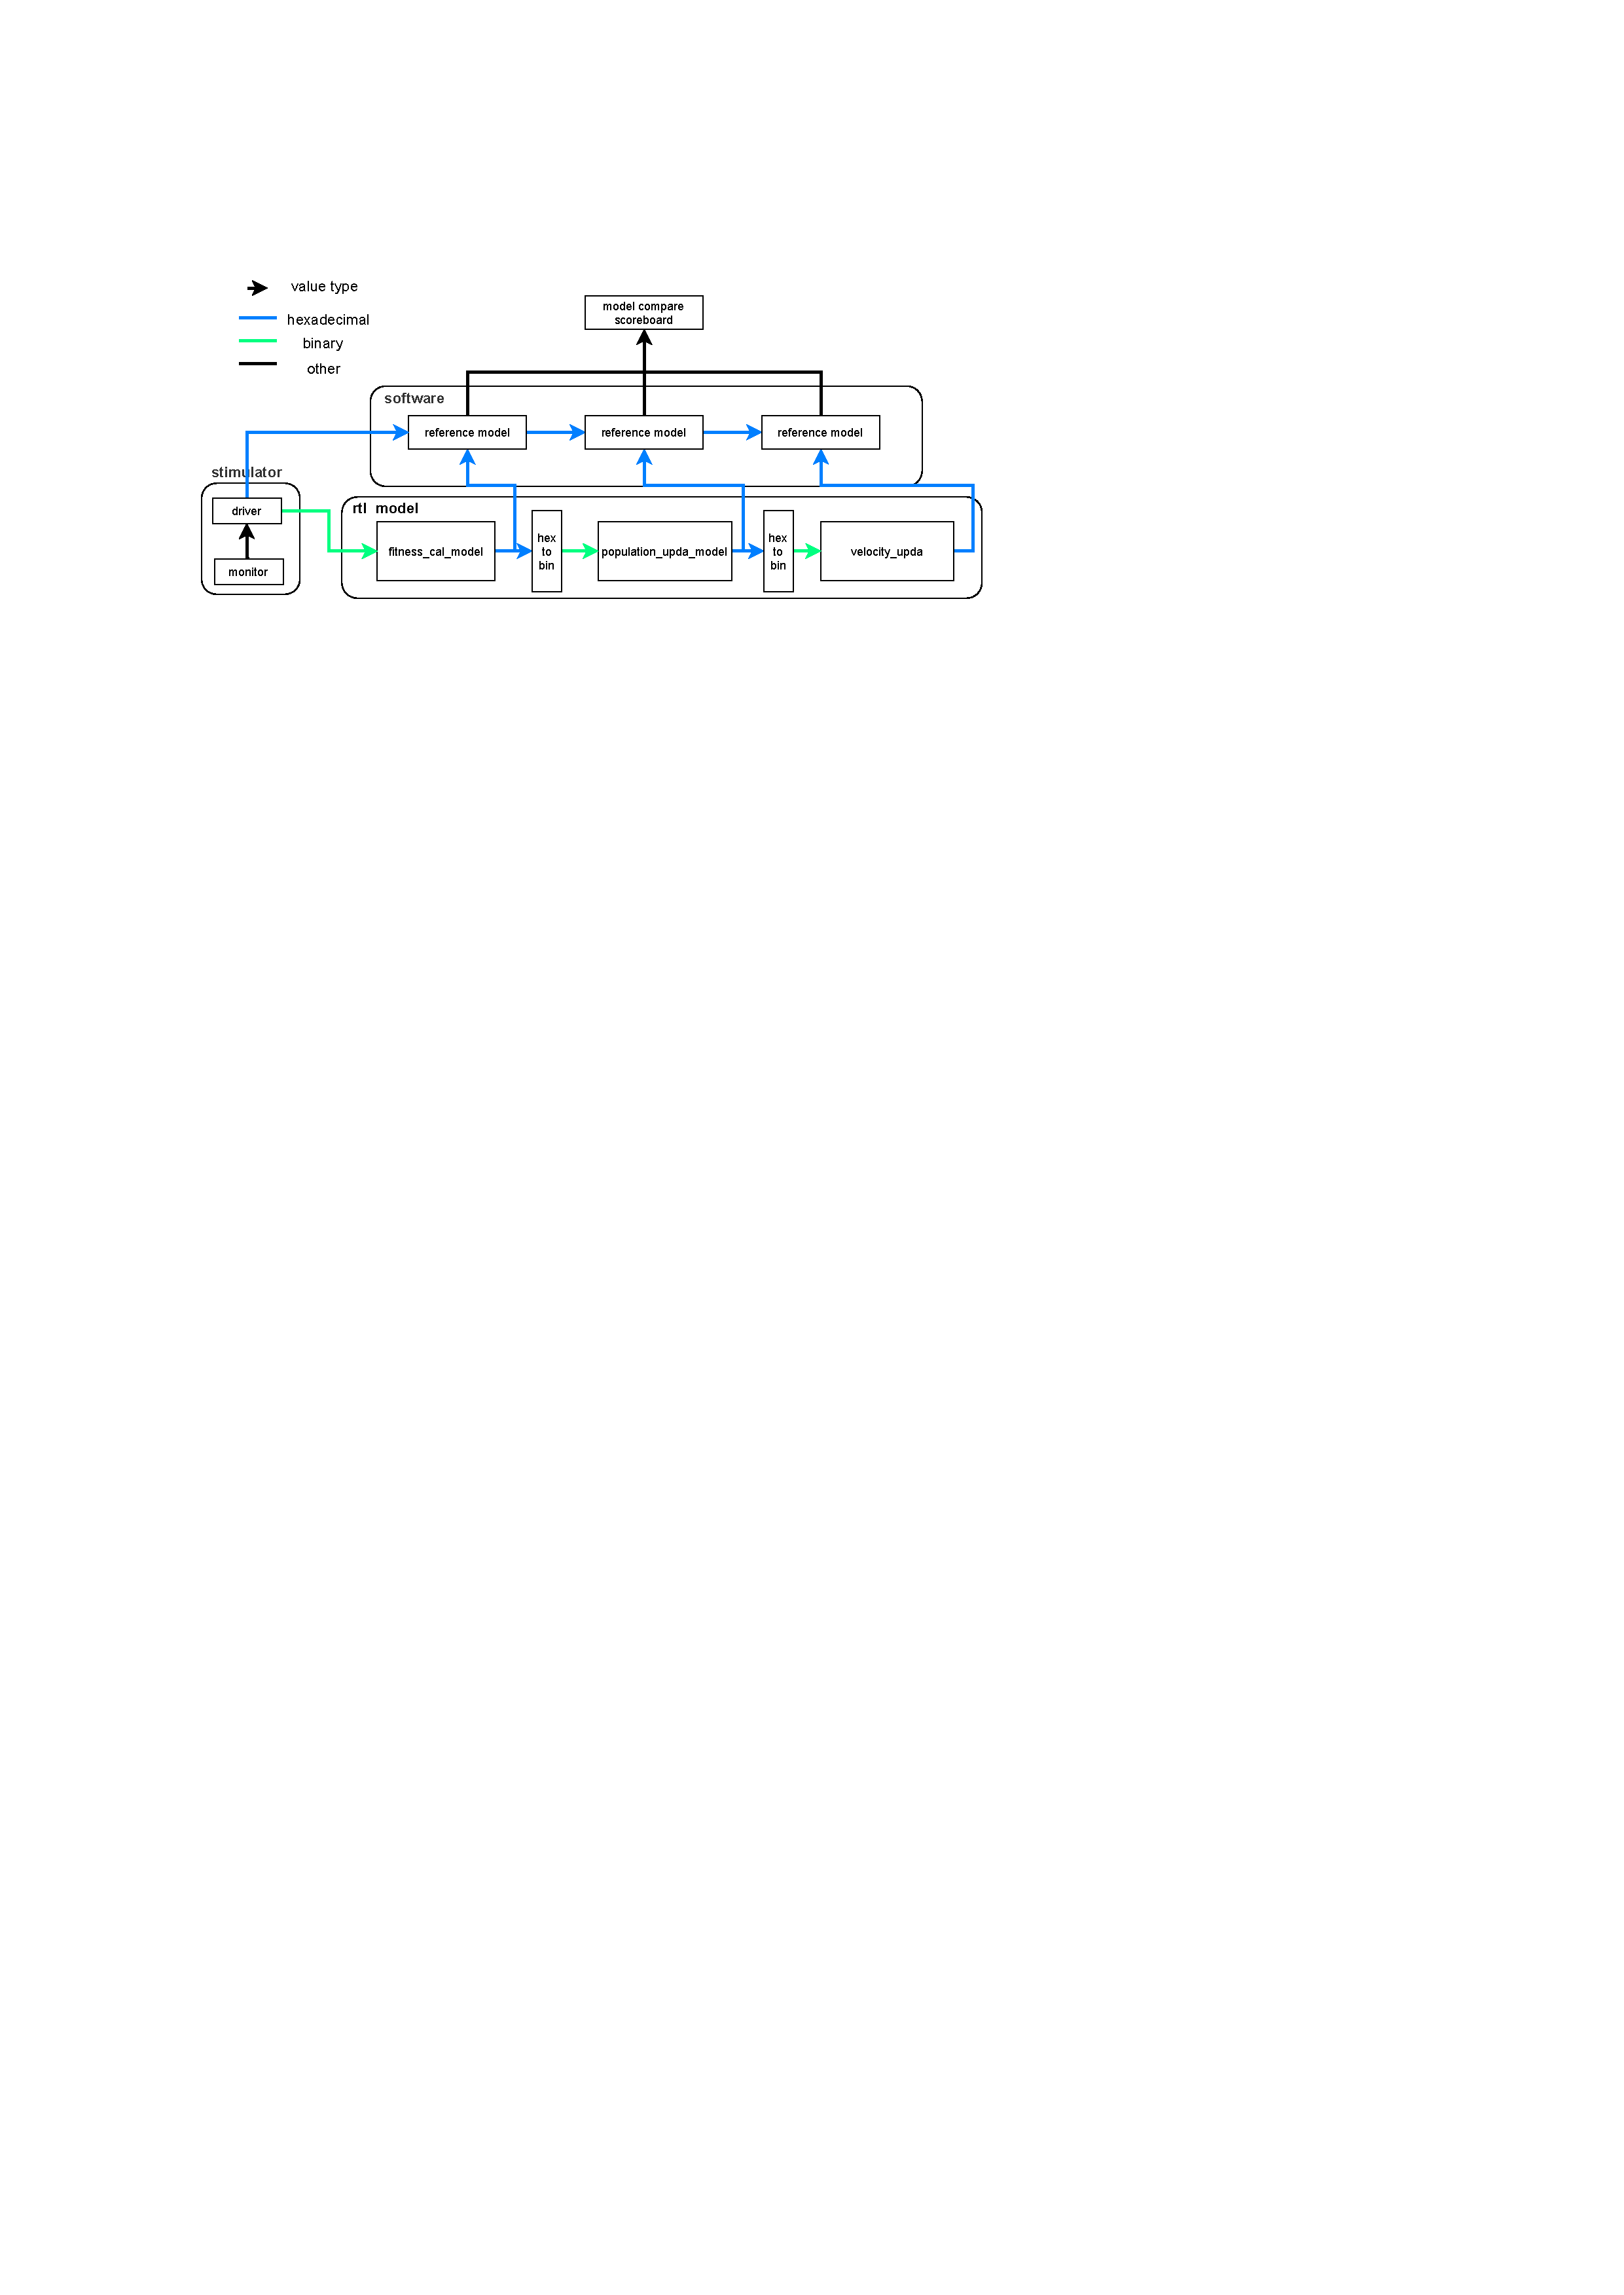
\includegraphics[width=14cm]{fig/4-fig/rtl_model验证环境.drawio.pdf}
  \caption{RTL model验证框架}
  \label{fig:RTL model验证框架}
\end{figure}

\subsection{验证激励和结果}
在单独模块的随机验证时(即每个模块的输入都是随机产生的,不来自上一模块,位移、温度、气压三个激励除外),激励产生约束如表所示。而在进行整个流水线的综合验证时,位移、气压和温度数据就采用实际的测量数据,初始搜索点则采用原始的Edlen公式,每一级模块的输入使用上一级模块的输出。
\begin{table}[H]
  \centering
  \caption{RTL model激励产生约束}
  \label{tab:RTL model激励产生约束}
  \begin{tabular}{c|c|c|c}
      \hline
      激励名                             & 激励意义                   &  数值范围       & 约束条件  \\ \hline
      fitness$\_$cal$\_$disp            & 输入的位移                  &  [-500,500]     & 无      \\ \hline
      fitness$\_$cal$\_$pres            & 输入的气压                  &  [-500,500]     & 无      \\ \hline
      fitness$\_$cal$\_$temp            & 输入的温度                  &  [-500,500]     & 无      \\ \hline
      fitness$\_$cal$\_$para            & 当前搜索点                  &  [-500,500]     & 无      \\ \hline
      population$\_$upda$\_$gbest       & 迭代结果的全局最优解         &  [0,5000]       & 无       \\ \hline
      population$\_$upda$\_$pbest       & 迭代结果的局部最优解         &  [0,5000]       &小于population$\_$upda$\_$pbest \\ \hline
      velocity$\_$upda$\_$curpara       & 上一轮迭代的位置信息         & [-500,500]      & 等于fitness$\_$cal$\_$para     \\ \hline
      velocity$\_$upda$\_$lastv         & 上一轮迭代的速度增量         & [0,1]           & 无     \\ \hline
      velocity$\_$upda$\_$randc         & 更新速度信息的随机数         & [0,1]           & 无     \\ \hline
  \end{tabular}
\end{table}

设定的最大误差阈值如下:population$\_$upda$\_$pbest模块的所有输出需要与software的输出完全一致,其余所有模块的输出的最大误差阈值为$\pm4\%$,误差产生的主要原因时上述的截断误差,截断误差虽然不大于0.0039,但截断误差一旦参与了乘法运算使得误差被放大,所以在这设定的阈值为$\pm4\%$。但需要特别强调的是,这$\pm4\%$的误差并不会给粒子群算法的结果带来太大影响,这是由于粒子群算法本身就有较大的随机性,从式\eqref{eq:粒子群算法速度更新}中两个随机数就可以看出,所以这个$\pm4\%$的误差只是又增加了一部分随机性而已,不会有太大影响。

单独模块的随机验产生了20组,每组2500个样本点,共计50000个激励测试点,而在整个流水线的综合验证时使用了所有的实际测量数据,所有验证结果的误差均为超过上述设定的阈值,可以认为算法的硬化达到了所需的要求。

\section{本章小结}
本章首先介绍了粒子群算法的基本原理以及本文使用的线性惯性权值递减策略,指出粒子群算法本身具有的早熟收敛问题,然后提出一种基于粒子群算法的优化的Edlen公式补偿方案,该方案将Edlen公式与粒子群算法相结合,不仅可以改善Edlen公式自身的温度不匹配、波长不匹配等问题,也可以解决粒子群算法自身早熟收敛的问题。并在第3章中的短时测量、长时测量和大范围温度变化测量中进行补偿,补偿效果较原始Edlen公式和整段式粒子群算法补偿方法均有不错的提升,但同时也在实验中发现当温度变化梯度过大时,线性形式的Edlen公式并不适用,为此又进行了其他实验,并且基于微积分的思想提出一种基于温度梯度的分段式粒子群算法补偿方法,实验验证该方法较原始Edlen公式和整段式粒子群算法补偿方法的效果均有提升,并且适用于较大温度变化梯度的情形。但该方法也有着一些不足之处,其中最为明显的时对粒子群算法的计算速度有较高的要求,为了解决该方法的不足,采用硬件加速的方法提升其运算速度,并介绍了算法的硬化方案,以及硬化算法正确性的验证框架,给出测试激励的产生条件和验证结果。

  \chapter{用于干涉仪环境补偿的粒子群算法的硬件加速补偿系统设计}
\section{硬件设计方法}
\subsection{流水线技术}
\label{流水线技术}
当前一般用吞吐率(throughput)作为硬件的性能指标,对于将要设计的用于干涉仪环境补偿的粒子群加速补偿模块,其吞吐率的计算公式可以使用下式:
\begin{equation}\label{eq:吞吐率计算}
    throughput = \frac{Operation}{second}=\frac{PSO}{instructions}\times \frac{instructions}{clock cycle} \times \frac{clock cycle}{time(1s)}.
    \end{equation}

式\eqref{eq:吞吐率计算}的含义为每秒钟能执行的操作数量,它由三部分组成:有效操作(PSO计算)占所有指令的比例$\frac{PSO}{instructions}$、每个周期能执行的指令数量$\frac{instructions}{clock cycle}$以及1秒钟内包含的周期个数$\frac{instructions}{clock cycle}$,其中前两项为强相关,可以合并为一个因素进行考虑,即一个周期能执行的PSO操作数量,所以最终决定设计出来的硬件的吞吐率的影响指标为:每个周期能执行的PSO操作数量和1秒钟内包含的周期个数。如果不采用流水线技术设计一个单周期的加速器,那么每一个周期能执行的PSO操作数量为1,但是由于一次PSO操作需要涉及到适应度计算、位置和速度更新、种群信息更新三个步骤,而这中间由涉及到很多乘法,这会导致设计出来的加速器的信号延迟很大,从而使得一个周期所需要的时间增加,一秒钟内包含的周期个数较少,最后设计出来的加速器的吞吐率较低,所以需要采用流水线技术。

流水线技术的本质就是通过插入寄存器,将一个较长的组合逻辑分割成多个较短的组合逻辑,并在每个组合逻辑中使用寄存器暂存数据,信号在一个周期内必须通过的路径长度减小了,系统的时钟周期就可以降低了。这就好像是在流水线上的工人,原本一件事情一个工人需要10秒钟才能完成,现在将这件事情分给10个工人去干,每个工人只需要1秒钟即可完成,这样就减少了所需要的时间,所以称为流水线技术。并且这并不会导致每个周期能执行的操作数量下降,为采用流水线技术时,一个周期能完成的PSO操作数量为1,现在采用5级流水线技术,假设所需要进行的PSO操作数量为N,那么一个周期能完成的PSO操作数量为$\frac{N}{N+5}$,根据极限的原理可知,当N足够大时,计算出来的结果仍为1。所以采用流水线技术,根据式\eqref{eq:吞吐率计算}可知,加速器的吞吐率即可以得到提升。流水线技术的示意图如下图所示。
\begin{figure}[htb]
    \centering
    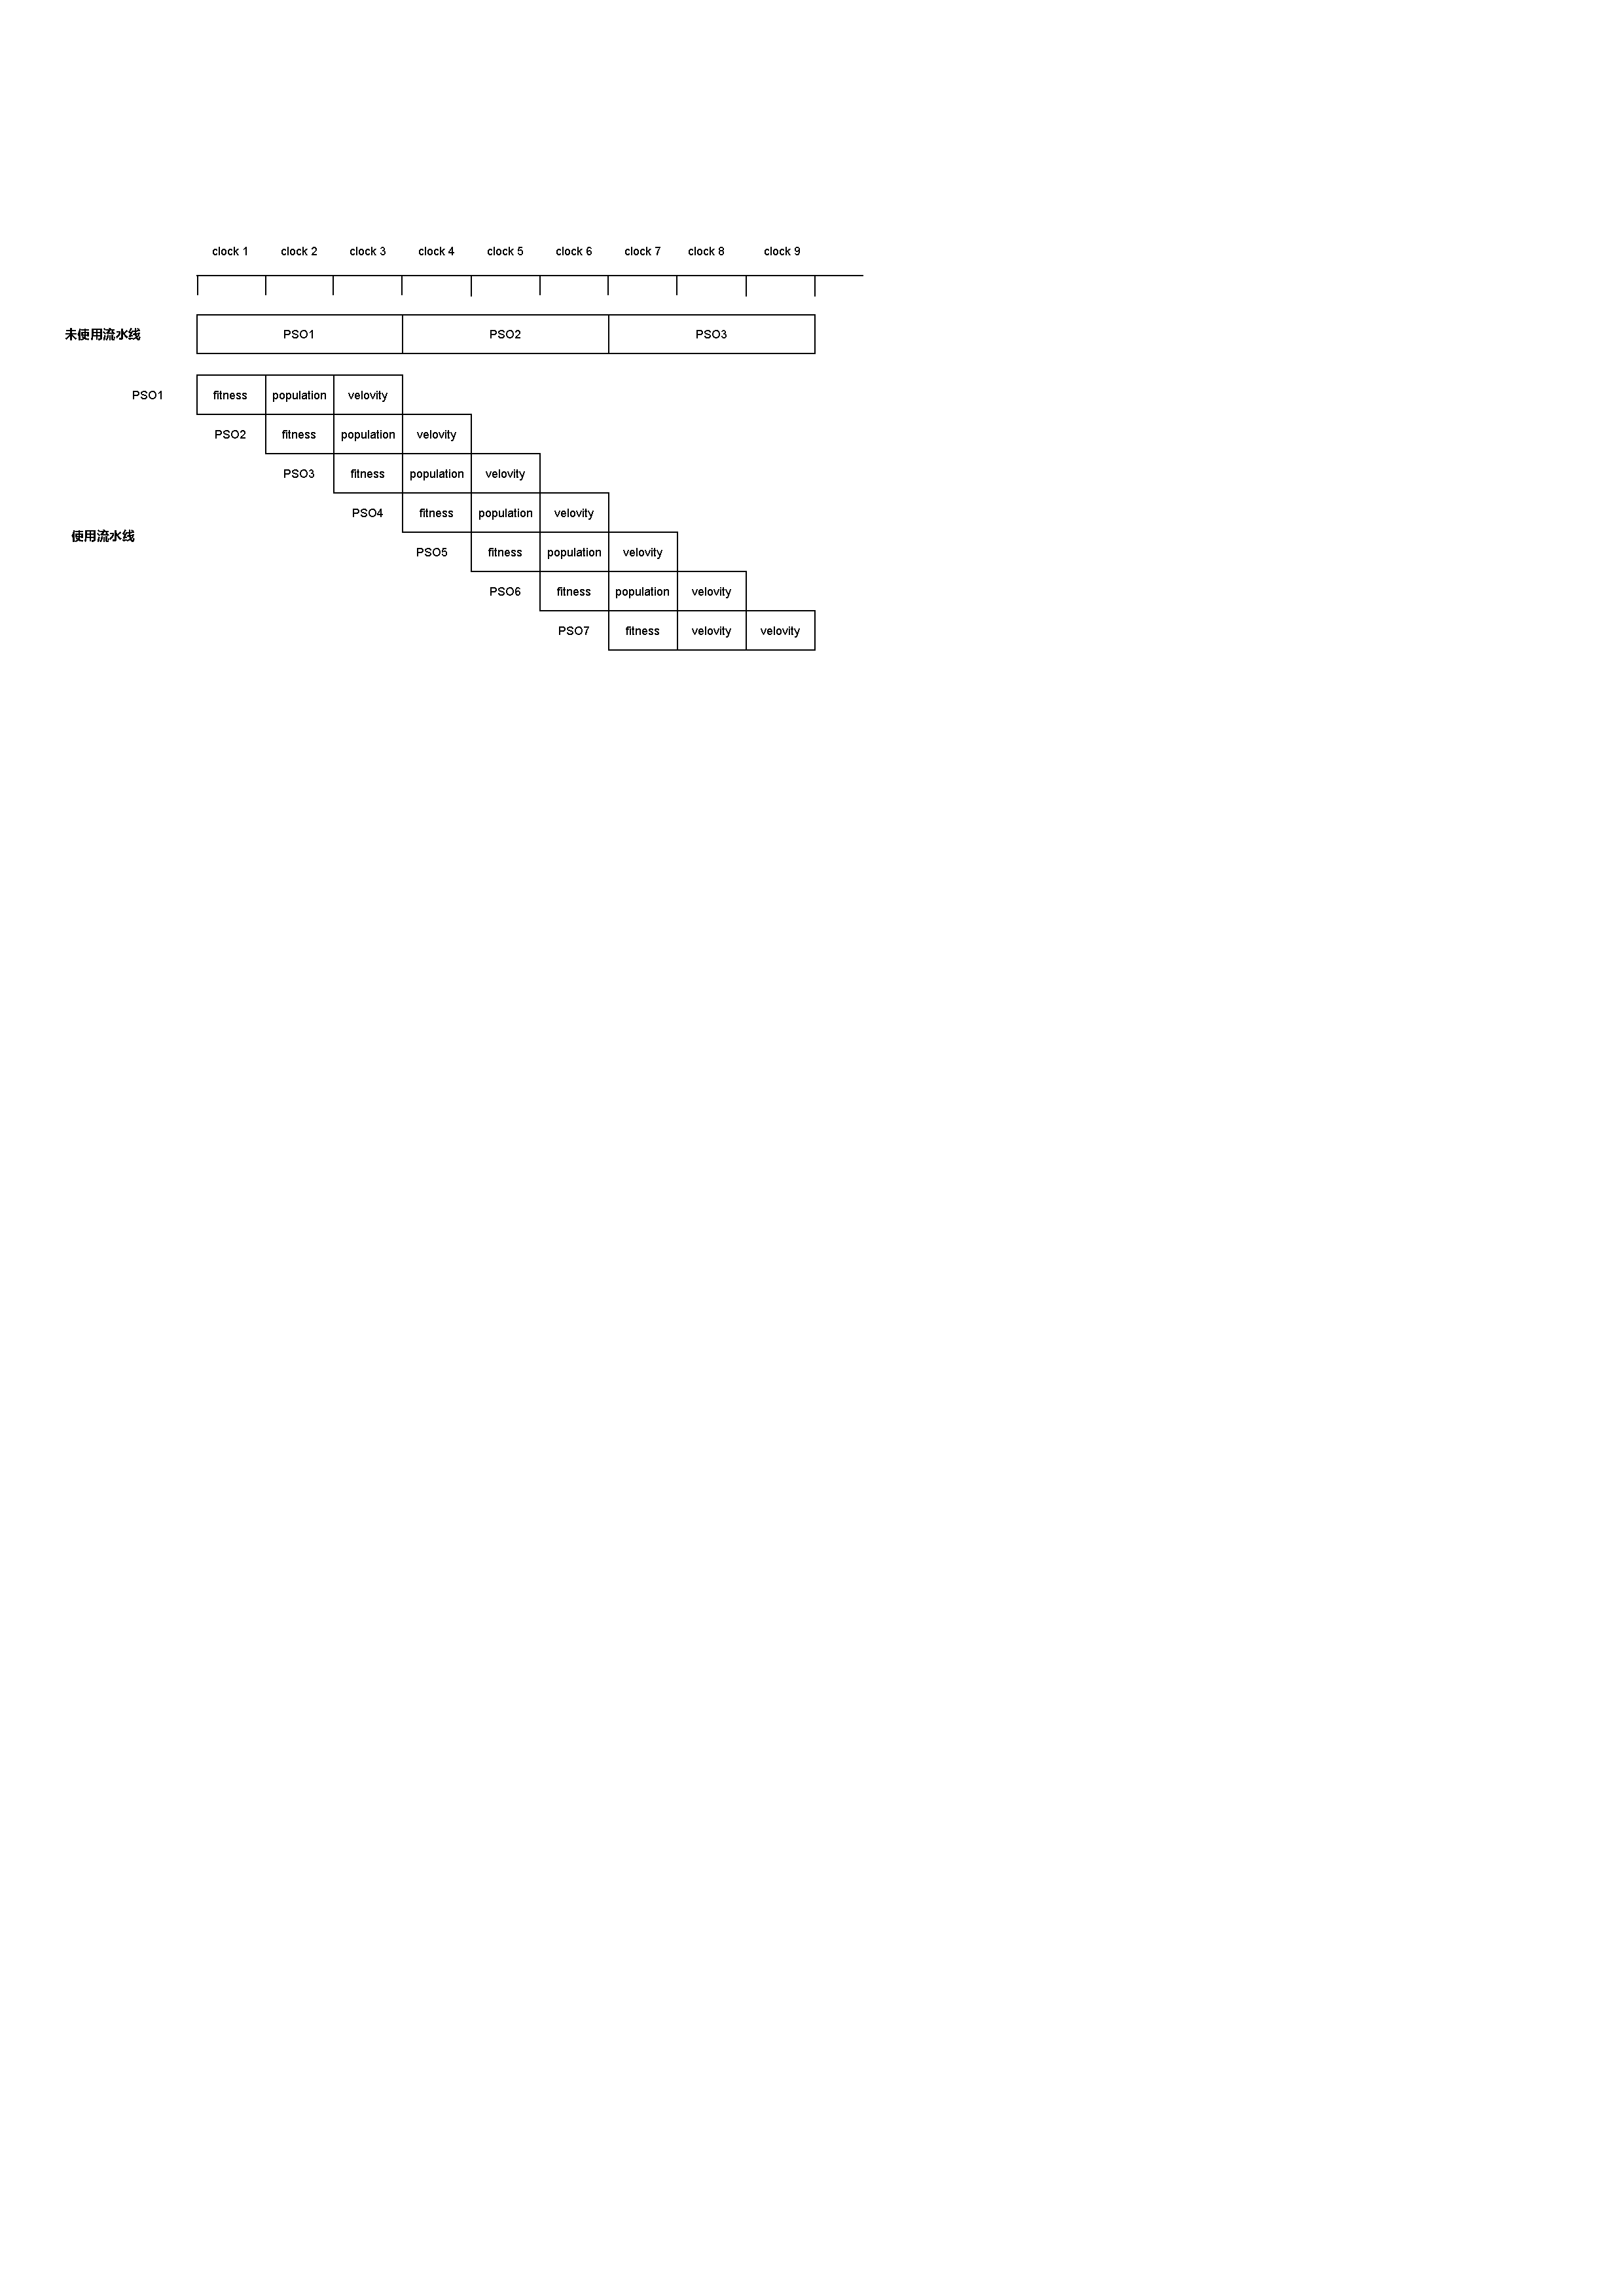
\includegraphics[width=14cm]{fig/5-fig/流水线示意图.drawio.pdf}
    \caption{流水线示意图}
    \label{fig:流水线示意图}
  \end{figure}

图\ref{fig:流水线示意图}画出了9个时钟周期内PSO操作情况,假设适应度计算(fitness)、速度和位置更新(velocity)以及种群信息更新(population)三个计算步骤需要的时间完全一致,都需要一个时钟周期,那么完成一次完整的PSO操作需要3个时钟周期。从图中可以看出,再未使用流水线技术时,9个时钟周期内使能完成3次PSO操作。如果采用了流水线技术,第一次PSO操作从第1个时钟周期开始,于第3个时钟周期完成,第二次PSO操作从第2个时钟周期开始,于第4个时钟周期结束,以此类推,可以看出在同一个时钟周期内,最多各只会有一次适应度计算、速度和位置更新以及种群信息更新,所以这不会引起硬件资源的冲突。采用流水线技术后,9个时钟周期内可以完成7次PSO操作,所以采用流水线技术可以很大程度上提升加速器的性能。

本文设计的用于干涉仪环境补偿的粒子群算法专用加速补偿系统为6级流水线,其中适应度计算模块由于含有大量乘法计算,所以设计为4级流水线,速度和位置更新以及种群信息更新模块乘法计算较少所以共为2级流水线。

\subsection{握手控制方案}
\label{握手控制方案}
由于采用了流水线技术,将一次PSO操作分成了多级流水完成,对于相邻的两级流水线,上一级的输出是下一级的输入,所以如果上一级的输出尚未准备好,那么下一级的流水线是无法进行计算的,需要被阻塞直至上一级流水线的输出准备就绪,或者如果上一级的输出已经准备好了,但是下一级处于忙碌状态无法接收数据,那么上一级的输出是没法给下一级流水的,需要阻塞到下一级流水空闲了再把数据下发。上述这些情形导致相邻两级的流水需要一组控制信号进行通信,这样相邻的两级流水线才能知道自己什么时候能正常工作,这组信号就被称为握手信号。

本文设计的用于干涉仪环境补偿的粒子群算法加速补偿系统的握手控制方案中共含有4个握手信号:in$\_$vld、in$\_$rdy、out$\_$vld、out$\_$rdy,各信号含义如表\ref{tab:握手信号含义表}所示。如果两级流水线之间是直连的,无其他任何逻辑,那么通常上一级流水的out$\_$vld和out$\_$rdy分别连接的是本级流水的in$\_$vld、in$\_$rdy,当in$\_$vld、in$\_$rdy同时为高时称为完成一次握手,此时可认为上一级流水输出的信号已经被本级流水所暂存,上一级流水可以继续进行其他运算了,具体的时序图如图\ref{fig:握手控制模块时序图}所示。
\begin{table}[H]
    \centering
    \caption{握手信号含义表}
    \label{tab:握手信号含义表}
    \begin{tabular}{c|c|c}
        \hline
        名称                               & 含义                   &  信号流向         \\ \hline
        in$\_$vld              & 上一级流水的输出信号是否有效           &上一级流水$\rightarrow$本级流水        \\ \hline
        in$\_$rdy              & 否能接收上一级流水的信号              &本级流水  $\rightarrow$上一级流水       \\ \hline
        out$\_$vld             & 本级流水的输出信号是否有效            & 本级流水 $\rightarrow$下一级流水       \\ \hline
        out$\_$rdy             & 下一级流水能否接收信号                & 下一级流水$\rightarrow$本级流水       \\ \hline
    \end{tabular}
  \end{table}

\begin{figure}[htb]
    \centering
    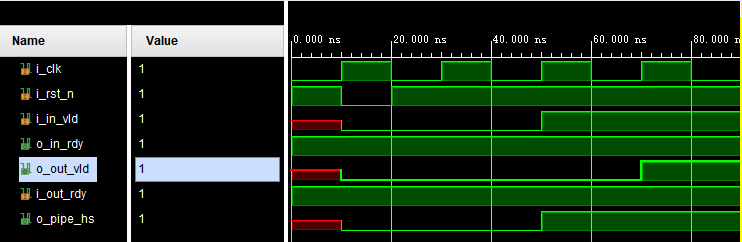
\includegraphics[width=14cm]{fig/5-fig/握手控制模块时序图.jpg}
    \caption{握手控制模块时序图}
    \label{fig:握手控制模块时序图}
\end{figure}

本文设计的流水线握手控制模块名称为pipe$\_$ctrl$\_$cell,其逻辑结构图为\ref{fig:握手控制模块逻辑结构图},其中i$\_$in$\_$vld即为上述的in$\_$vld信号,i表明这个信号对于pipe$\_$ctrl$\_$cell为输入信号(input),i$\_$rst$\_$n为模块的复位信号,i$\_$clk为模块的时钟信号,o$\_$pipe$\_$hs为成功握手信号。一个pipe$\_$ctrl$\_$cell模块需要的FPGA资源如表\ref{tab:握手控制模块资源消耗表}所示,主要使用到的资源为查找表(Look-Up-Table,简称LUT)以及寄存器。
\begin{figure}[htb]
    \centering
    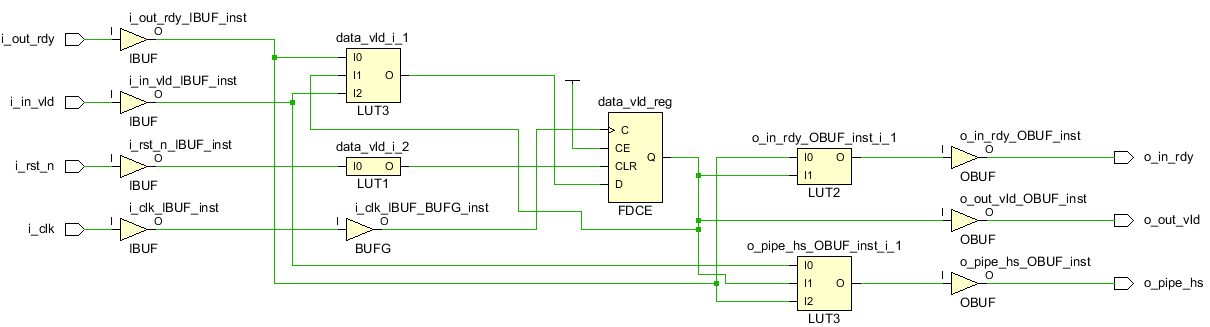
\includegraphics[width=14cm]{fig/5-fig/握手控制模块逻辑结构图.jpg}
    \caption{握手控制模块逻辑结构图}
    \label{fig:握手控制模块逻辑结构图}
  \end{figure}

  \begin{table}[H]
    \centering
    \caption{握手控制模块资源消耗表}
    \label{tab:握手控制模块资源消耗表}
    \begin{tabular}{c|c}
        \hline
        资源类别             & 数量  \\ \hline
        Slice LUTs          & 3     \\ \hline
        Slice Register      & 1     \\ \hline
        Bonded IOB          & 7     \\ \hline
        BUFGCTRL            & 1     \\ \hline
    \end{tabular}
  \end{table}

  \subsection{逻辑复制与资源共享技术}
  逻辑复制技术指的是在硬件设计的过程中,如果某级流水后负载过多,而且该处又为关键信号,就可以通过使用逻辑复制技术,将该处电路复制一份以降低该关键信号的扇出从而降低该关键信号的延迟,这样就可以提高电路的性能。在用于干涉仪环境补偿的粒子群算法加速补偿系统的设计过程中,如果设置的种群个体数过多,由式\eqref{eq:粒子群算法速度更新}和式\eqref{eq:粒子群算法位置新}可以看出在进行每个个体的速度位置更新时所需的$pbest_i$和$gbest$都来源于种群信息更新模块,这就会导致种群信息更新模块后的负载过多而使得其延迟过大,所以可以对其采用逻辑复制技术,采用逻辑复制技术前后如如图\ref{fig:逻辑复制技术示意图}所示。
  \begin{figure}[htb]
    \centering
    \subfigure[未使用逻辑复制]{
      \begin{minipage}[b]{0.99\textwidth}
        \centering
        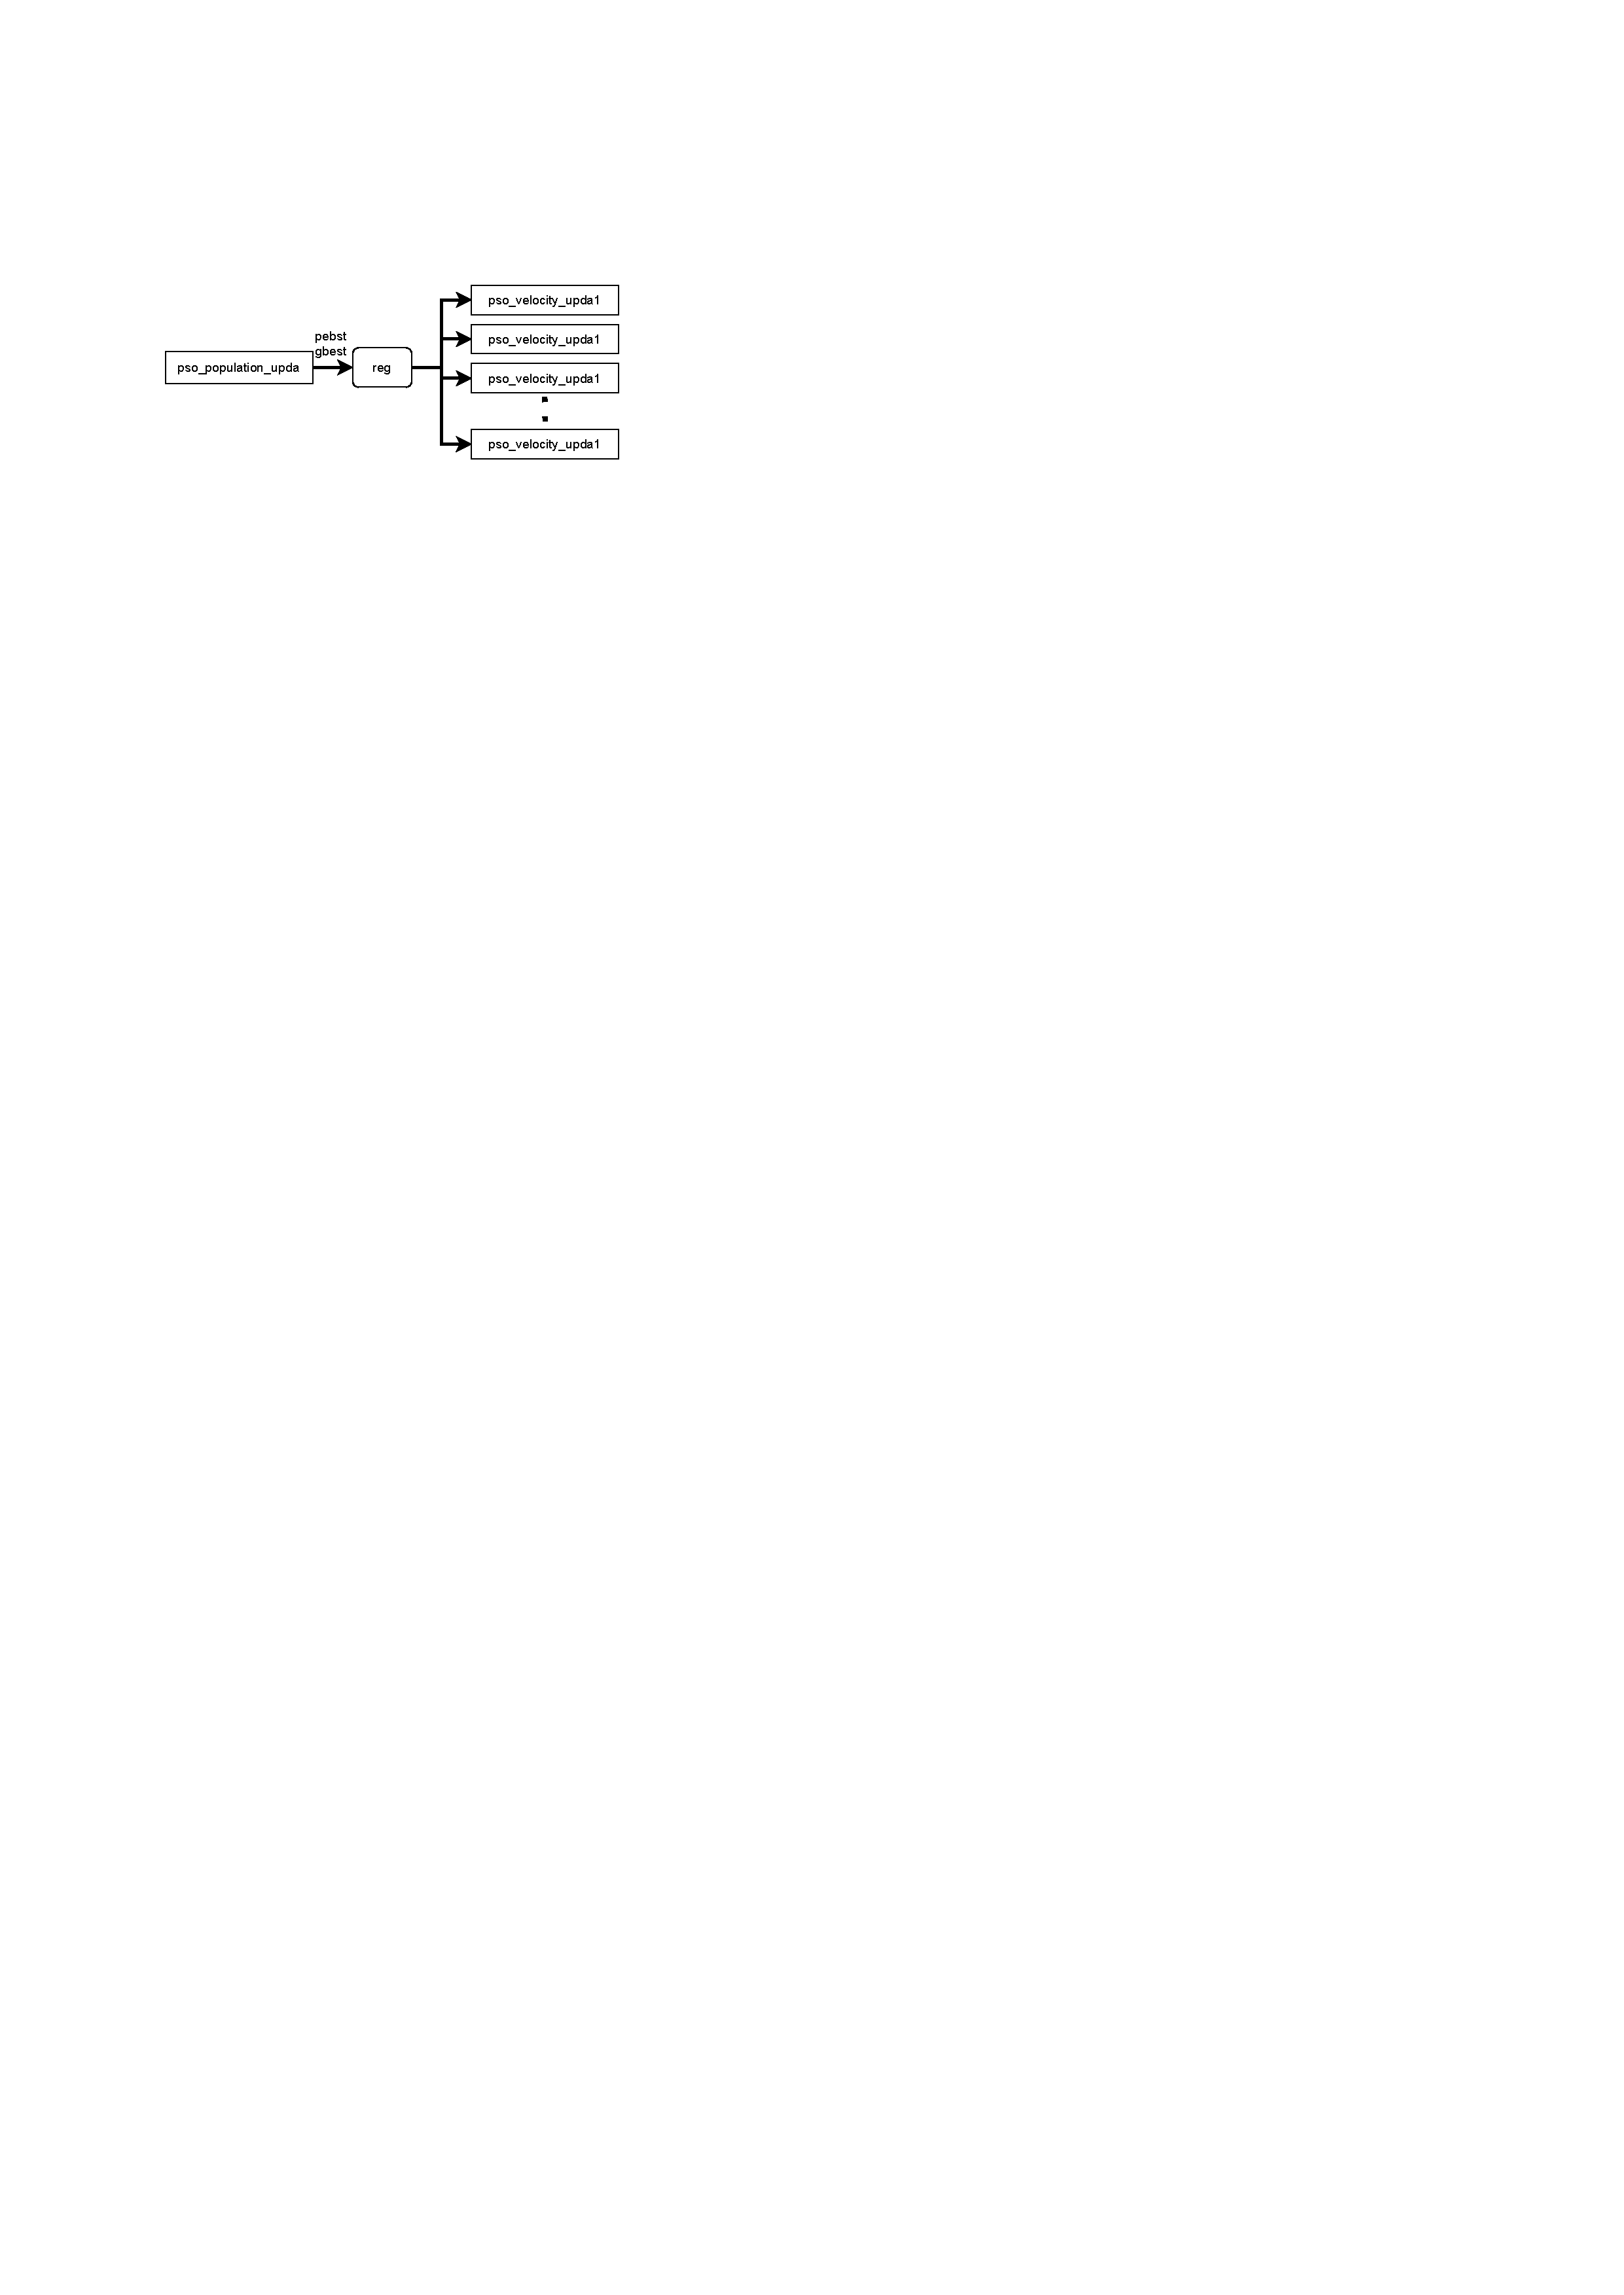
\includegraphics[width=8.5cm,height=3.3cm]{fig/5-fig/逻辑复制示意图a.drawio.pdf}
      \end{minipage}
      \label{fig:未使用逻辑复制}
    }
    \subfigure[使用逻辑复制]{
      \begin{minipage}[b]{0.99\textwidth}
        \centering
        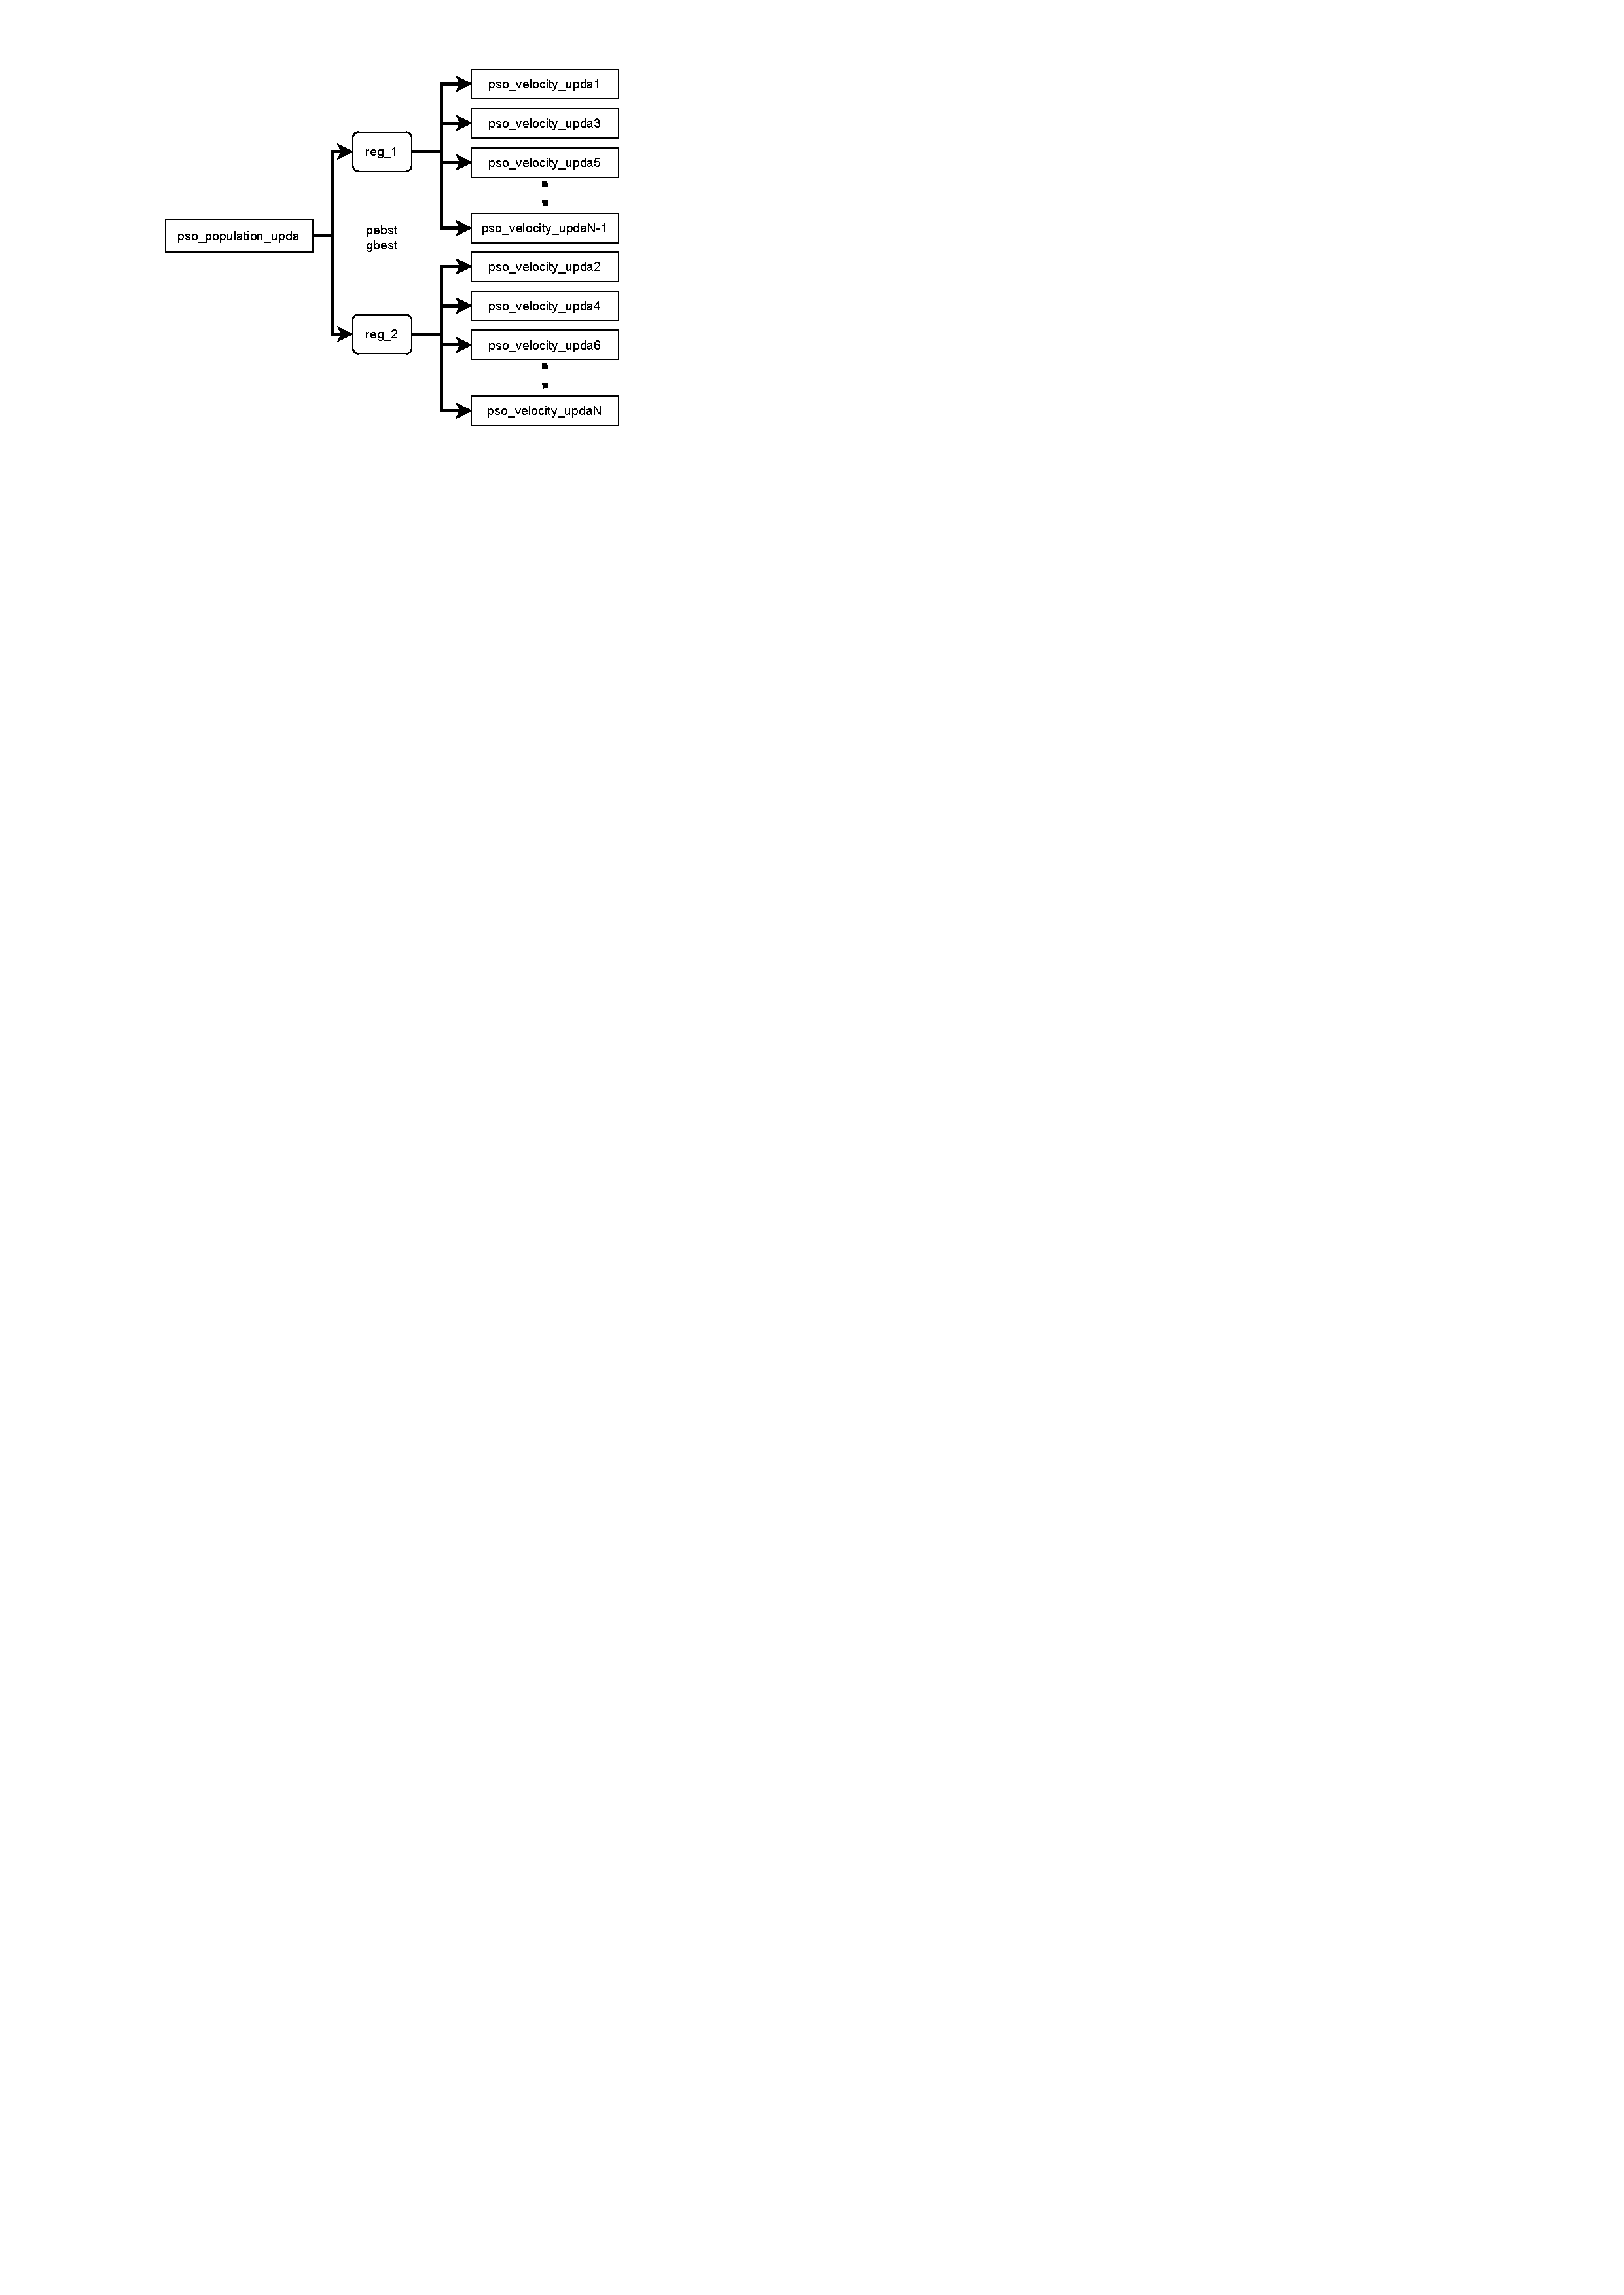
\includegraphics[width=8.8cm,height=6.4cm]{fig/5-fig/逻辑复制示意图b.drawio.pdf}
      \end{minipage}
      \label{fig:使用逻辑复制}
    }
    \caption{逻辑复制技术示意图}
    \label{fig:逻辑复制技术示意图}
  \end{figure}

  资源共享技术则是与逻辑复制技术相反,在不影响性能的非关键路径上,如果存在比较多的公共单元,则可以多个电路共同使用同一个公共单元,这么做可能会导致延时增大,但由于不是关键路径,所以影响较小,但这可以减小面积。

\subsection{门控时钟技术}
对于电路而言,其功耗主要分为两类:静态功耗的动态功耗。静态功耗又可以叫做待机功耗,它主要是由于电路中的漏电流导致的功耗,其计算公式如式\eqref{eq:静态功耗计算公式}所示,其中$I_s$为静态工作电流,$V_{DD}$为工作电压。而动态功耗又可以叫做开关功耗,它是由于逻辑翻转所产生的功耗,即电平发生$0\rightarrow1$和$1\rightarrow0$跳变时所产生的功耗,其计算方法如式\eqref{eq:动态功耗计算公式}所示,式中$C_L$为寄生电容,$S$为每个时钟周期内电路的平均翻转次数,$f_{clk}$为时钟频率。而由于现在FPGA的时钟频率一般为几十MHz到几百MHz,这意味着时钟每秒会发生几千万次到几亿次的跳变,所以由时钟翻转带来的功耗是很大的。减少这部分功耗最简单的方法就是:判断每个模块是否处于工作状态,如果不处于工作状态则将该模块的输入的时钟关闭,这种技术称为门控时钟技术。
\begin{equation}\label{eq:静态功耗计算公式}
    P_s = I_s \times V_{DD}.
    \end{equation}
\begin{equation}\label{eq:动态功耗计算公式}
    P_{dynamic}=SC_LV^2_{DD}f_{clk}.
    \end{equation}


为了判断每个模块是否处在工作状态,需要在每个模块的I/O中新增一个信号:busy,该信号为1代表该模块处于工作状态,为0则说明该模块处于空闲状态,最简单的方法就是将busy信号和时钟信号clk相与,这样当模块处于空闲状态的时候,与门输出的结果就一直是0,就将时钟关断了,如果模块正在工作,busy信号为1,clk$\&$busy的结果仍然是clk,不会影响模块的正常工作。但是由于与门是电平逻辑,所以一旦busy信号有毛刺,就会导致经过门控时钟出来之后的时钟也有毛刺,而导致时钟信号错误的关断,这对电路的功能是致命的。所以当前门控时钟一般采用锁存门控或者寄存门控,这两种方法采用锁存器/寄存器对busy信号进行暂存,能很有效地避免毛刺造成干扰。本文使用锁存门控技术,其结构图和波形图如图\ref{fig:锁存门控的结构图和波形图}所示。$clk\_in$为原始时钟,$clk\_out$为经过时钟门控之后的模块输入时钟。
\begin{figure}[htb]
    \centering
    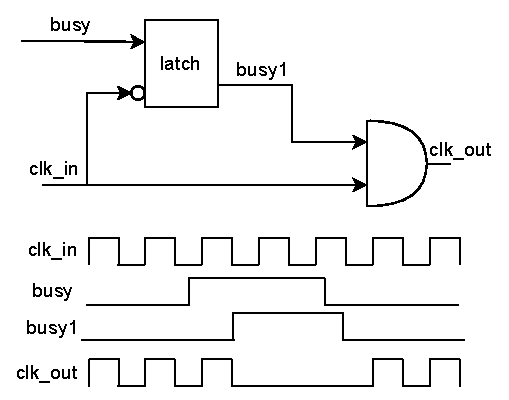
\includegraphics[width=8cm]{fig/5-fig/锁存门控的结构图和波形图.drawio.pdf}
    \caption{锁存门控的结构图和波形图}
    \label{fig:锁存门控的结构图和波形图}
\end{figure}

\subsection{随机数生成设计}
由于数字电路中只存在0和1两个值,并且要求任一时刻电路都处于确定的状态,并无中间态产生,否则会进入亚稳态,这导致对于数字电路而言,随机数的生成是一件非常困难的事情,电路生成的随机数大多都是伪随机数,即只在一定范围内进行随机,并且有规律可循。本文在随机数生成的设计上采用线性反馈移位寄存器(Linear Feedback Shift Register,简称LSFR),LSFR由若干个触发器和异或门组成,其原理是使用反馈函数改变LSFR中现存的序列,并将反馈函数的输出进行移位,从而在一定的序列长度内可以生成源源不断的伪随机输出。本文设计的随机数生成模块名称为pso$\_$lsfr$\_$rangen,其架构图如图\ref{fig:LSFR架构图}所示,这是一个8位的LSFR,反馈系数为101110001,所能产生的最大不重复序列的长度为$2^8-1=255$种,所以它能产生的最大255个随机值,并通过seed控制随机值的产生顺序。
\begin{figure}[htb]
    \centering
    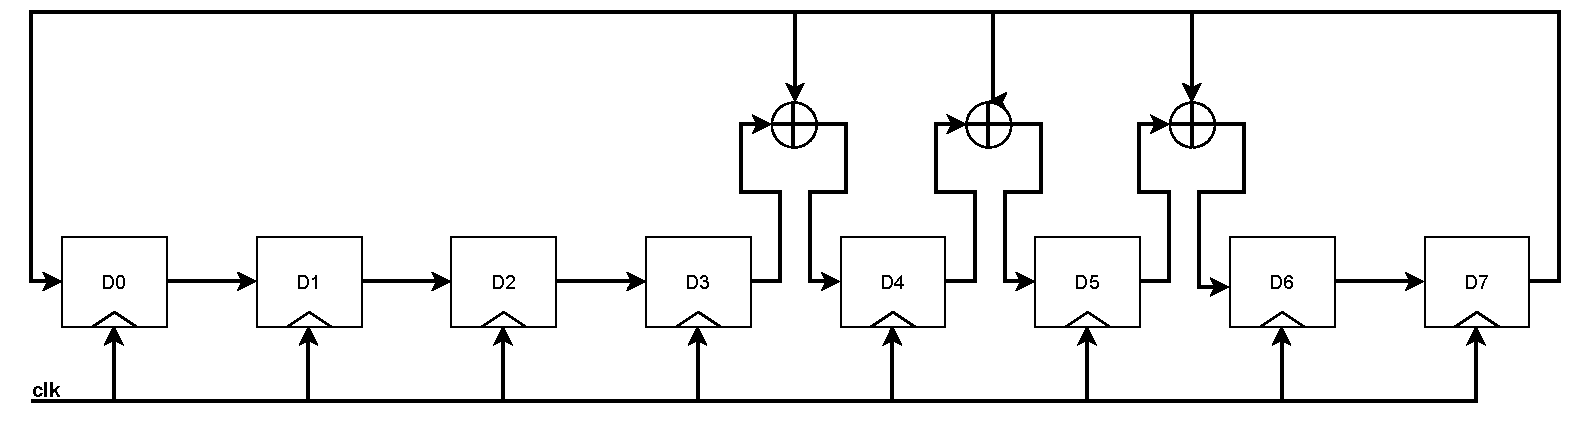
\includegraphics[width=14cm]{fig/5-fig/LSFR架构图.pdf}
    \caption{LSFR架构图}
    \label{fig:LSFR架构图}
\end{figure}

\section{粒子群算法加速补偿系统架构}
整个粒子群算法加速补偿系统架构如图\ref{fig:粒子群算法加速补偿系统架构示意图},其中pipe$\_$ctrl$\_$cell为\ref{握手控制方案}节中介绍的握手控制模块,pso$\_$fitness$\_$cal为适应度计算模块,并行放置了N个适应度计算模块,pso$\_$population$\_$upda为种群信息更新模块,pso$\_$velocity$\_$cal为速度和位置更新模块,也共放置了N个模块用于并行加速。

\begin{figure}[htb]
    \centering
    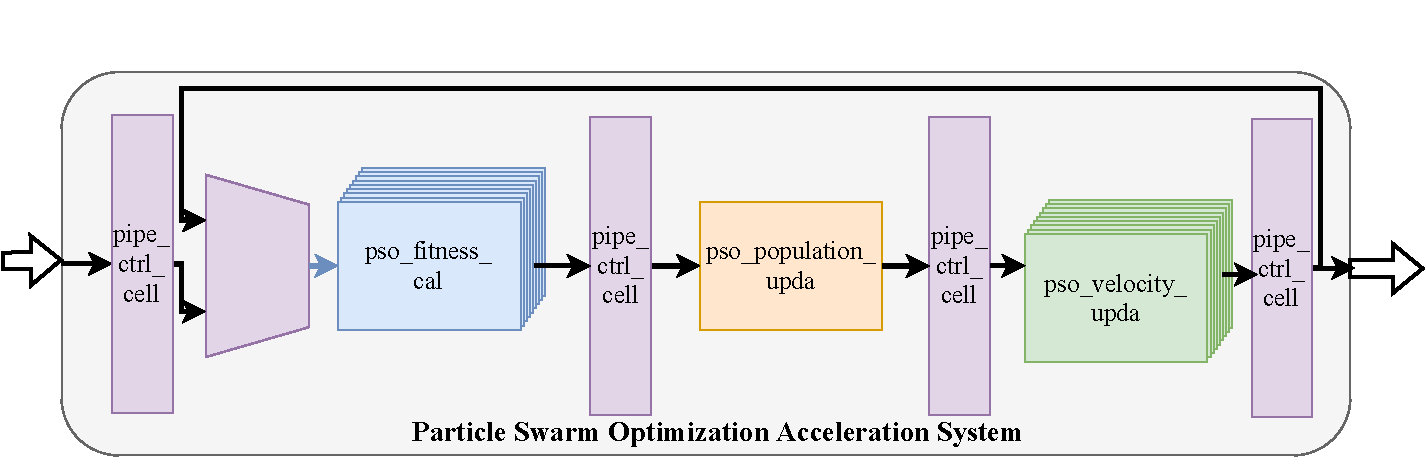
\includegraphics[width=14cm]{fig/5-fig/粒子群算法加速系统架构.drawio.pdf}
    \caption{粒子群算法加速补偿系统架构}
    \label{fig:粒子群算法加速补偿系统架构示意图}
\end{figure}

为了兼顾硬件的灵活性和可维护性,某些可配置信息不使用寄存器配置方法,而采用parameter方法配置,具体参数含义及默认值如表\ref{tab:parameter定义表}所示。
\begin{table}[H]
    \centering
    \caption{parameter定义表}
    \label{tab:parameter定义表}
        \begin{tabular}{c|c|c}
        \hline
        名称          & 含义                            & 默认值     \\ \hline
        SAM$\_$NUM    & 训练的样本数量,推荐为2的幂次方   & 128           \\ \hline
        IND$\_$NUM    & 种群的个体数量,推荐为2的幂次方   & 32            \\ \hline
        PARA$\_$NUM   & 待训练参数数量                  & 2      \\ \hline
        GEN$\_$NUM    & 迭代上限次数,推荐为2的幂次方    & 256       \\ \hline
        IW            & 整数部分位宽                    & 16      \\ \hline
        FW            & 小数部分位宽                    & 8     \\ \hline
    \end{tabular}
  \end{table}

整个粒子群算法加速补偿系统的接口信号如表\ref{tab:粒子群算法加速补偿系统接口信号表}所示,给出了顶层所有接口的名称、方向、位宽以及含义。其中$i\_$或$o\_$的前缀表明该信号是输入还是输出,$\_$cfg$\_$标志代表是一个寄存器接口,$\_$pso$\_$标志代表是系统的数据或控制信号输入,其余为系统的全局信号。
\begin{table}[H]
    \centering
    \caption{粒子群算法加速补偿系统接口信号表}
    \label{tab:粒子群算法加速补偿系统接口信号表}
    \begin{tabular}{c|c|c|c}
        \hline
        接口名                                       & 接口方向  & 位宽               &含义                         \\ \hline
        i$\_$clk                                    & 输入      & 1                     & 系统时钟信号              \\ \hline
        i$\_$rst$\_$n                               & 输入      & 1                     & 系统复位信号   \\ \hline
        i$\_$flush                                  & 输入      & 1                     & 系统刷新信号              \\ \hline
        i$\_$cfg$\_$pso$\_$in$\_$initial$\_$para    & 输入      & PARA$\_$NUM*(IW+FW)   & 训练起点                 \\ \hline
        i$\_$cfg$\_$pso$\_$in$\_$initial$\_$lastv   & 输入      & PARA$\_$NUM*(IW+FW)   & 训练的初始速度            \\ \hline
        i$\_$cfg$\_$pso$\_$in$\_$len                & 输出      & 8                     & 测量臂长度                \\ \hline
        i$\_$cfg$\_$pso$\_$start                    & 输入      & 1                     & 系统开始信号              \\ \hline
        o$\_$cfg$\_$pso$\_$busy                     & 输出      & 1                     & 系统忙碌标志位            \\ \hline
        o$\_$cfg$\_$pso$\_$done                     & 输出      & 1                     & 计算完成信号              \\ \hline
        i$\_$pso$\_$in$\_$vld                       & 输入      & 1                     & 输入的有效信号            \\ \hline
        o$\_$pso$\_$in$\_$rdy                       & 输出      & 1                     & 输入接收准备信号          \\ \hline
        i$\_$pso$\_$in$\_$sample$\_$temp            & 输入      & SAM$\_$NUM*(IW+FW)    & 输入的温度数据            \\ \hline
        i$\_$pso$\_$in$\_$sample$\_$pres            & 输入      & SAM$\_$NUM*(IW+FW)    & 输入的气压数据            \\ \hline
        i$\_$pso$\_$in$\_$sample$\_$disp            & 输入      & SAM$\_$NUM*(IW+FW)    & 输入的位移数据            \\ \hline
        o$\_$pso$\_$out$\_$vld                      & 输出      & 1                     & 输出的有效信号            \\ \hline
        i$\_$pso$\_$out$\_$rdy                      & 输入      & 1                     & 输出接收准备信号          \\ \hline
        o$\_$pso$\_$trained$\_$temp                 & 输出      & (IW+FW)               & 训练后的温度因子          \\ \hline
        o$\_$pso$\_$trained$\_$pres                 & 输出      & (IW+FW)               & 训练后的气压因子          \\ \hline
    \end{tabular}
  \end{table}

\subsection{适应度计算模块架构}
适应度计算模块的架构如图\ref{fig:适应度计算模块架构图}所示的四级流水结构,图中也画出了大致的数据流,其中refractive$\_$cal为折射率计算,其计算方法如式\eqref{eq:线性形式的Edlen公式},compensation $\_$value为补偿值计算,其计算方法如式\eqref{eq:环境误差公式};error$\_$cal为适应度计算,其计算方法跟式\eqref{eq:均方根误差计算公式}类似,但是由于数字电路比较难实现算数平方根操作,所以将式中的算术平方根变为绝对值。要实现绝对值操作需要用到多个比较器,首先需要判断两个数符号位的关系,然后再判断数值位的大小关系,结合两次判断的结果得出两个数之间的大小关系,然后进行减法以实现绝对值操作。reg则代表相邻两级相邻流水线之间暂存数据的寄存器堆,虚线框表示的monitor为监视器,主要是为适应度计算模块每级流水验证时提供比对值。
  \begin{figure}[htb]
    \centering
    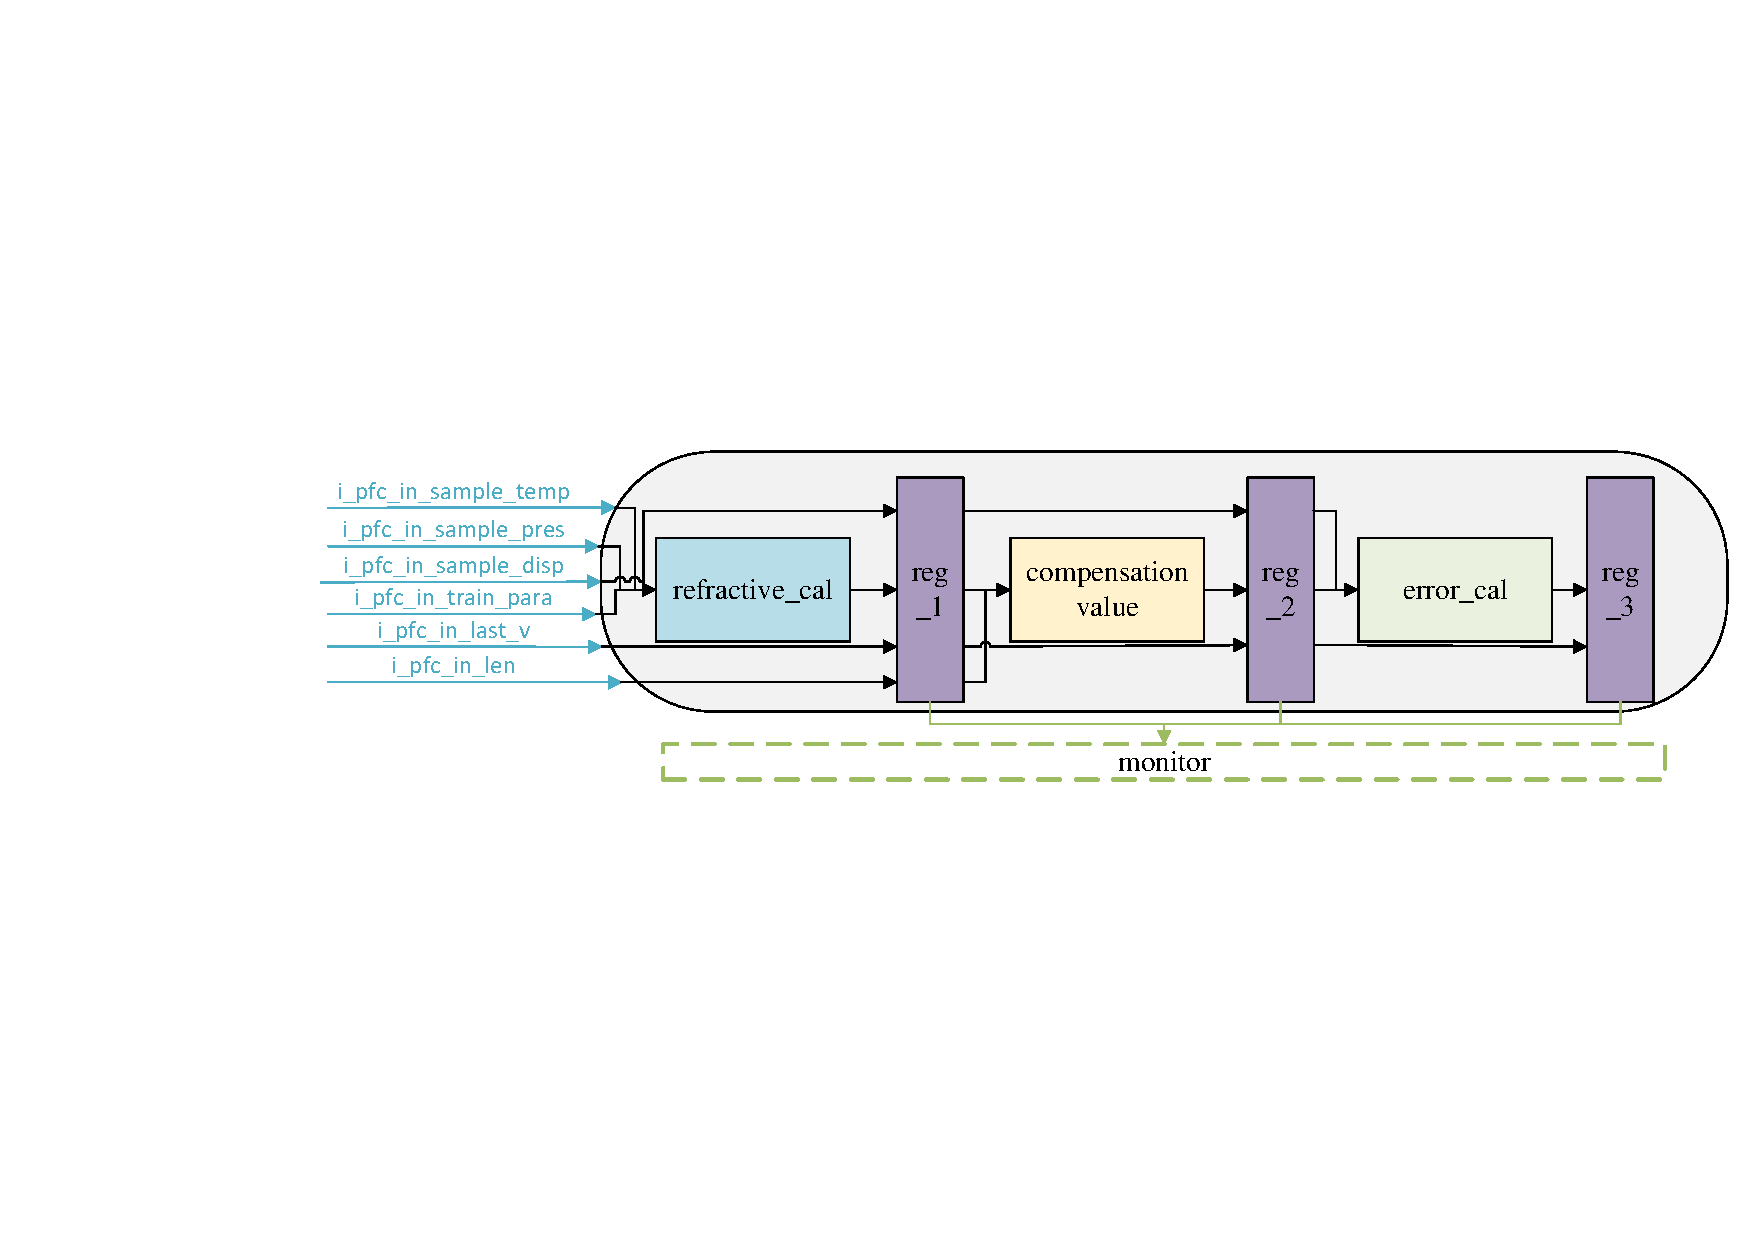
\includegraphics[width=14cm]{fig/5-fig/适应度计算模块架构图.pdf}
    \caption{适应度计算模块架构图}
    \label{fig:适应度计算模块架构图}
\end{figure}

适应度计算模块的所有接口信号如表\ref{tab:适应度计算模块接口信号表}所示,其中pfc为pso$\_$fitness$\_$cal的缩写首字母,标志着该信号为适应度计算模块的接口。
\begin{table}[H]
    \centering
    \caption{适应度计算模块接口信号表}
    \label{tab:适应度计算模块接口信号表}
    \begin{tabular}{c|c|c|c}
        \hline
        接口名                               & 接口方向  & 位宽               &含义                        \\ \hline
        i$\_$clk                            & 输入      & 1                     & 模块时钟信号             \\ \hline
        i$\_$rst$\_$n                       & 输入      & 1                     & 模块复位信号             \\ \hline
        i$\_$flush                          & 输入      & 1                     & 模块刷新信号             \\ \hline
        i$\_$pfc$\_$in$\_$vld               & 输入      & 1                     & 模块输入的有效信号        \\ \hline
        o$\_$pfc$\_$in$\_$rdy               & 输出      & 1                     & 模块输入的准备信号        \\ \hline
        i$\_$pfc$\_$in$\_$sample$\_$temp    & 输入      & SAM$\_$NUM*(IW+FW)    & 模块输入的温度数据        \\ \hline
        i$\_$pfc$\_$in$\_$sample$\_$pres    & 输入      & SAM$\_$NUM*(IW+FW)    & 模块输入的气压数据        \\ \hline
        i$\_$pfc$\_$in$\_$sample$\_$disp    & 输入      & SAM$\_$NUM*(IW+FW)    & 模块输入的位移数据        \\ \hline
        i$\_$pfc$\_$in$\_$train$\_$para     & 输入      & PARA$\_$NUM*(IW+FW)   & 模块输入的当前训练参数     \\ \hline
        i$\_$pfc$\_$in$\_$last$\_$v         & 输入      & PARA$\_$NUM*(IW+FW)   & 模块输入的当前速度        \\ \hline
        i$\_$pfc$\_$in$\_$len               & 输入      & 8                     & 模块输入的测量臂长度      \\ \hline
        o$\_$pfc$\_$out$\_$vld              & 输出      & 1                     & 模块输出的有效信号        \\ \hline
        i$\_$pfc$\_$out$\_$rdy              & 输入      & 1                     & 模块输出的准备信号        \\ \hline
        o$\_$pfc$\_$out$\_$busy             & 输出      & 1                     & 模块工作标志位            \\ \hline
        o$\_$pfc$\_$out$\_$train$\_$para    & 输出      & PARA$\_$NUM*(IW+FW)   & 模块输出的当前训练参数     \\ \hline
        o$\_$pfc$\_$out$\_$last$\_$v        & 输出      & PARA$\_$NUM*(IW+FW)   & 模块输出的当前速度         \\ \hline
        o$\_$pfc$\_$out$\_$fitness          & 输出      & IW+IW+FW+8            & 模块输出的适应度结果       \\ \hline
    \end{tabular}
  \end{table}

\subsection{种群信息更新模块架构}
种群信息更新模块的架构如图\ref{fig:适应度计算模块架构图}所示的二流水结构,图中也画出了大致的数据流。其中32to1是找出32个个体适应度最小的那一个,并找出该个体对应的两个训练参数,其结构为5级比较器,其中第一级有16个二选一的比较器,从32组数据中找出较小的16组数据,第二级有8个二选一比较器,第三级有4个,以此类推,在最后一级比较器的输出即可选中32组数据中个体适应度最小的一组。

global$\_$upda是比较32to1中找出的最小适应度值,跟模块本身记录的最小适应度值相比较,如果32to1中的适应度小,则将模块记录的适应度值进行更新;person$\_$upda是将32个种群个体分开判断,比较当前周期的计算的适应度值是否比模块自身的记录的适应值小,如果小则进行更新。global$\_$upda和person$\_$upda都是使用一个寄存器和一个比较器组合搭建的。reg则代表相邻两级相邻流水线之间暂存数据的寄存器堆,虚线框表示的monitor为监视器,主要是用于验证时提供比对值。


\begin{figure}[htb]
    \centering
    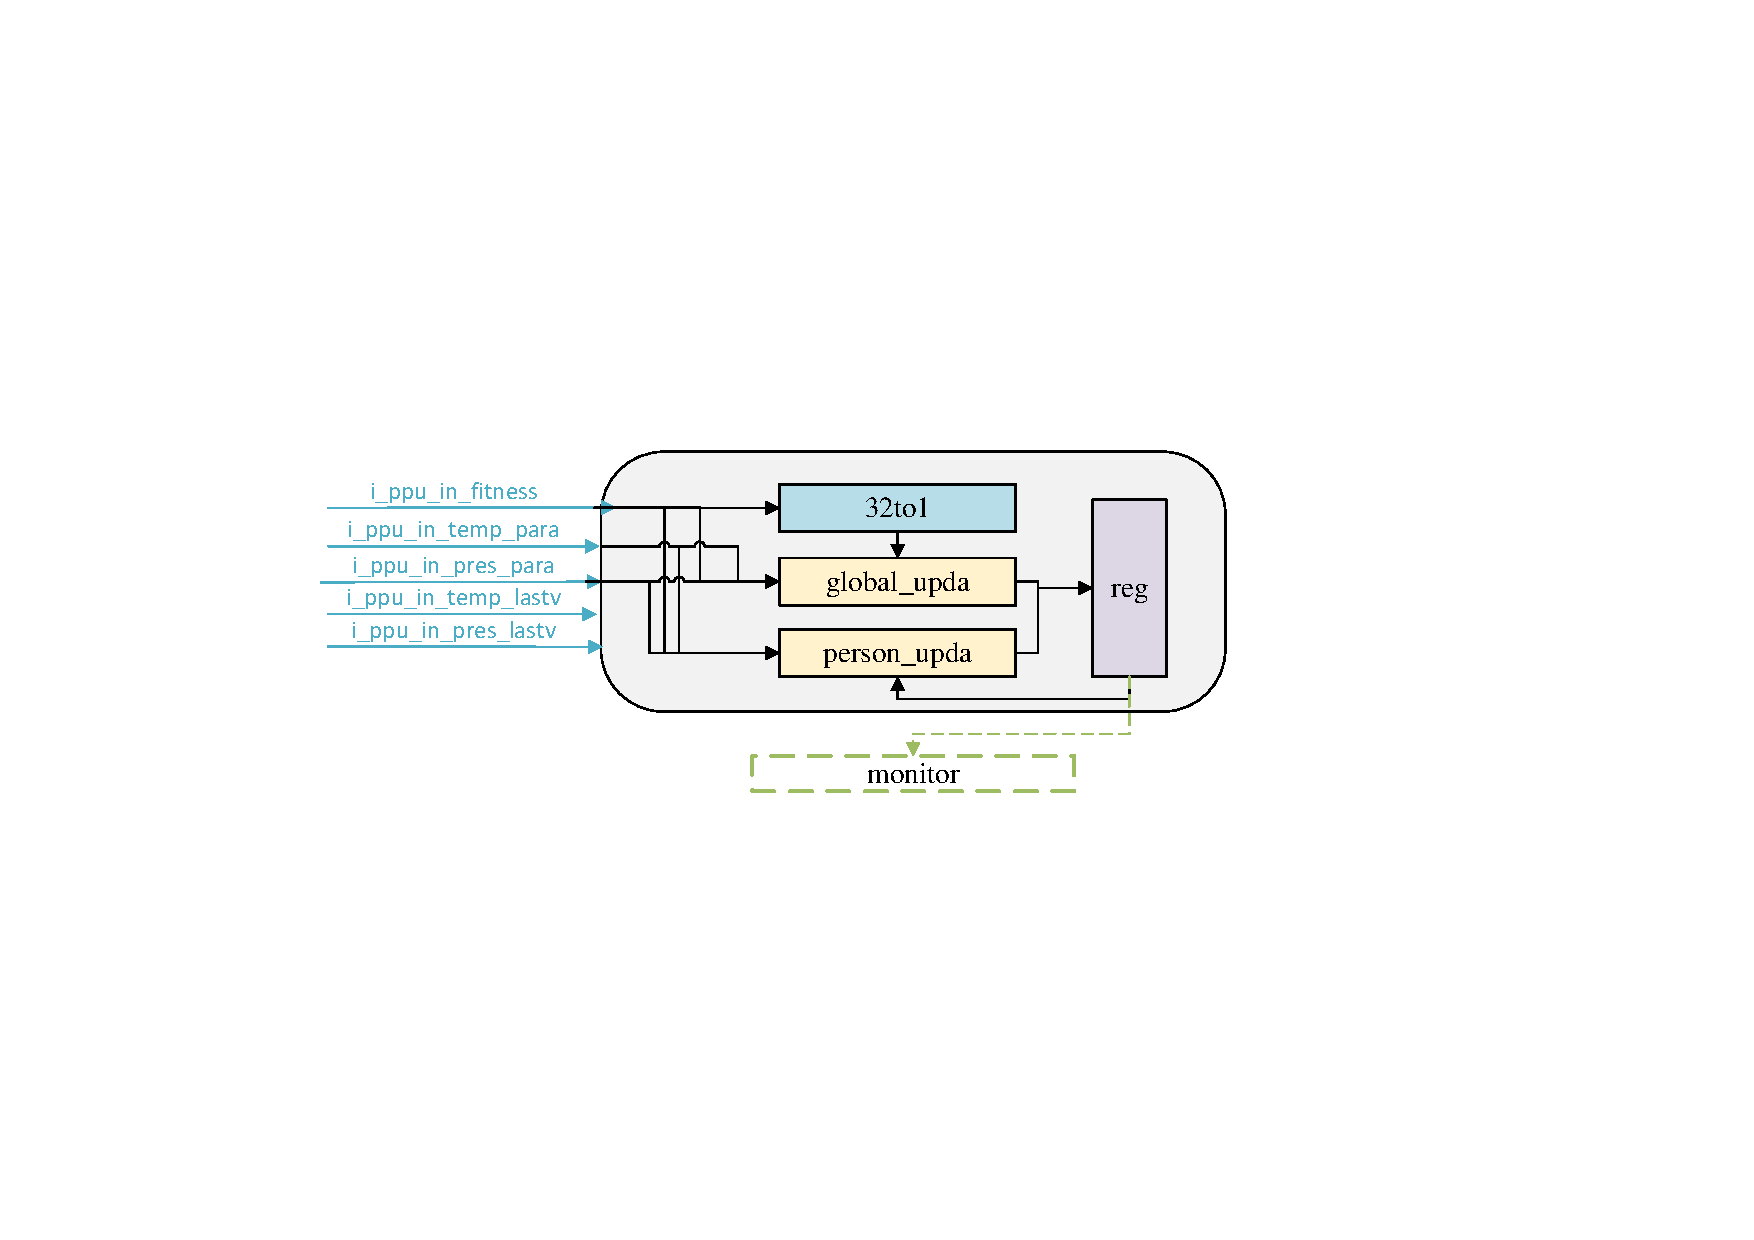
\includegraphics[width=10cm]{fig/5-fig/种群信息更新模块架构.pdf}
    \caption{种群信息更新模块架构}
    \label{fig:种群信息更新模块架构}
\end{figure}

种群信息更新模块的所有接口信号如表\ref{tab:种群信息更新模块接口信号表}所示,其中ppu为pso$\_$population$\_$upda的缩写首字母,标志着该信号为种群信息更新模块的接口。
\begin{table}[H]
    \centering
    \caption{种群信息更新模块接口信号表}
    \label{tab:种群信息更新模块接口信号表}
    \begin{tabular}{c|c|c|c}
        \hline
        接口名                               & 接口方向  & 位宽               &含义                        \\ \hline
        i$\_$clk                                       & 输入      & 1                     & 模块时钟信号             \\ \hline
        i$\_$rst$\_$n                                  & 输入      & 1                     & 模块复位信号             \\ \hline
        i$\_$flush                                     & 输入      & 1                     & 模块刷新信号             \\ \hline
        i$\_$ppu$\_$in$\_$vld                          & 输入      & 1                     & 模块输入的有效信号        \\ \hline
        o$\_$ppu$\_$in$\_$rdy                          & 输出      & 1                     & 模块输入的准备信号        \\ \hline
        i$\_$ppu$\_$in$\_$fitness                      & 输入      & IND$\_$NUM*(2*IW+FW+8) & 模块输入的适应度          \\ \hline
        i$\_$ppu$\_$in$\_$temp$\_$para                 & 输入      & IND$\_$NUM*(IW+FW)    & 模块输入的温度参数        \\ \hline
        i$\_$ppu$\_$in$\_$pres$\_$para                 & 输入      & IND$\_$NUM*(IW+FW)    & 模块输入的气压参数        \\ \hline
        i$\_$ppu$\_$in$\_$temp$\_$lastv                & 输入      & IND$\_$NUM*(IW+FW)    & 模块输入的温度速度        \\ \hline
        i$\_$ppu$\_$in$\_$pres$\_$lastv                & 输入      & IND$\_$NUM*(IW+FW)    & 模块输入的气压速度       \\ \hline

        o$\_$ppu$\_$out$\_$vld                         & 输出      & 1                     & 模块输出的有效信号        \\ \hline
        i$\_$ppu$\_$out$\_$rdy                         & 输入      & 1                     & 模块输出的准备信号        \\ \hline
        o$\_$ppu$\_$out$\_$temp$\_$para                & 输出      & IND$\_$NUM*(IW+FW)    & 模块输出的温度参数        \\ \hline
        o$\_$ppu$\_$out$\_$pres$\_$para                & 输出      & IND$\_$NUM*(IW+FW)    & 模块输出的气压参数        \\ \hline
        o$\_$ppu$\_$out$\_$temp$\_$lastv               & 输出      & IND$\_$NUM*(IW+FW)    & 模块输出的温度速度        \\ \hline
        o$\_$ppu$\_$out$\_$pres$\_$lastv               & 输出      & IND$\_$NUM*(IW+FW)    & 模块输出的气压速度        \\ \hline
        o$\_$ppu$\_$out$\_$global$\_$temp              & 输出      & (IW+FW)               & 全局最优温度参数        \\ \hline
        o$\_$ppu$\_$out$\_$global$\_$pres              & 输出      & (IW+FW)               & 全局最优气压参数        \\ \hline
        o$\_$ppu$\_$out$\_$person$\_$temp              & 输出      & IND$\_$NUM*(IW+FW)    & 个体最优温度参数        \\ \hline
        o$\_$ppu$\_$out$\_$person$\_$pres              & 输出      & IND$\_$NUM*(IW+FW)    & 个体最优气压参数        \\ \hline
    \end{tabular}
  \end{table}

\subsection{速度和位置更新模块架构}
速度和位置更新模块架构的架构如图\ref{fig:速度和位置更新模块架构图}所示的二流水结构,图中也画出了大致的数据流。其中LSFR1和LSFR为2个8位的线性反馈移位寄存器,用于产生式\eqref{eq:粒子群算法速度更新}中的两个随机数,velocity$\_$upda和position$\_$upda分别为计算式\eqref{eq:粒子群算法速度更新}和\eqref{eq:粒子群算法位置新}。reg则代表相邻两级相邻流水线之间暂存数据的寄存器堆,虚线框表示的monitor为监视器,主要是用于验证时提供比对值。
\begin{figure}[htb]
    \centering
    \includegraphics[width=14cm]{fig/5-fig/速度和位置更新模块架构图.pdf}
    \caption{速度和位置更新模块架构图}
    \label{fig:速度和位置更新模块架构图}
\end{figure}

速度和位置更新模块的所有接口信号如表\ref{tab:速度和位置更新模块接口信号表}所示,其中pvc为pso$\_$velocity$\_$cal的缩写首字母,标志着该信号为速度和位置更新模块的接口。

\begin{table}[H]
    \centering
    \caption{速度和位置更新模块接口信号表}
    \label{tab:速度和位置更新模块接口信号表}
\begin{tabular}{c|c|c|c}
    \hline
    接口名                                          & 接口方向  & 位宽               &含义                        \\ \hline
    i$\_$clk                                       & 输入      & 1                     & 模块时钟信号             \\ \hline
    i$\_$rst$\_$n                                  & 输入      & 1                     & 模块复位信号             \\ \hline
    i$\_$flush                                     & 输入      & 1                     & 模块刷新信号             \\ \hline
    i$\_$pvc$\_$in$\_$vld                          & 输入      & 1                     & 模块输入的有效信号        \\ \hline
    o$\_$pvc$\_$in$\_$rdy                          & 输出      & 1                     & 模块输入的准备信号        \\ \hline
    i$\_$pvc$\_$in$\_$cur$\_$para                  & 输入      & PARA$\_$NUM*(IW+FW)   & 模块输入的当前训练参数         \\ \hline
    i$\_$pvc$\_$in$\_$global$\_$temp               & 输出      & (IW+FW)               & 模块输入全局最优温度参数        \\ \hline
    i$\_$pvc$\_$in$\_$global$\_$pres               & 输出      & (IW+FW)               & 模块输入全局最优气压参数        \\ \hline
    i$\_$pvc$\_$in$\_$person$\_$temp               & 输出      & IND$\_$NUM*(IW+FW)    & 模块输入个体最优温度参数        \\ \hline
    i$\_$pvc$\_$in$\_$person$\_$pres               & 输出      & IND$\_$NUM*(IW+FW)    & 模块输入个体最优气压参数        \\ \hline
    i$\_$pvc$\_$in$\_$lsfr$\_$seed1                & 输入      & 8                     & 模块输入的随机种子              \\ \hline
    i$\_$pvc$\_$in$\_$lsfr$\_$seed2                & 输入      & 8                     & 模块输入的随机种子              \\ \hline


    o$\_$pvc$\_$out$\_$vld                         & 输出      & 1                     & 模块输出的有效信号        \\ \hline
    i$\_$pvc$\_$out$\_$rdy                         & 输入      & 1                     & 模块输出的准备信号        \\ \hline
    o$\_$pfc$\_$out$\_$nxt$\_$para                 & 输出      & PARA$\_$NUM*(IW+FW)   & 模块输出的更新训练参数     \\ \hline
    o$\_$pfc$\_$out$\_$nxt$\_$v                    & 输出      & PARA$\_$NUM*(IW+FW)   & 模块输出的更新速度         \\ \hline

\end{tabular}
\end{table}

\subsection{多起点训练方法及寄存器配置}
常规的粒子群算法一般都是单起点训练的,但是由于本文提出的温度梯度的分段式粒子群算法补偿方法中在温度变化梯度过大触发一次分段训练时,采用的粒子群算法的训练起点是上一次的训练的训练结果,如\ref{温度梯度的分段式粒子群算法补偿方法}节所述,这就导致了设计的粒子群加速补偿系统需要支持多起点训练,同时在\ref{流水线技术}节中也说明了整个粒子群算法加速补偿系统是一个6级流水线的设计,如果只用1个起点进行训练是无法覆盖整个流水线的初始延迟,其波形如图\ref{fig:单起点训练时序图}所示。
\begin{figure}[htb]
    \centering
    \includegraphics[width=14cm]{fig/5-fig/单起点训练时序图.jpg}
    \caption{单起点训练时序图}
    \label{fig:单起点训练时序图}
\end{figure}

从图中可以看出由于流水线较深使得如果只从一个起点开始训练,每个模块仍然有较长的空闲状态,硬件的利用率较低,这与流水线设计的初衷相悖,所以采用多起点进行训练则可以很好地解决这个问题。
\begin{figure}[htb]
    \centering
    \includegraphics[width=14cm]{fig/5-fig/多起点训练时序图.jpg}
    \caption{多起点训练时序图}
    \label{fig:多起点训练时序图}
\end{figure}

如图\ref{fig:多起点训练时序图}所示,由于是一个6级流水线的设计,所以将训练起点个数设为5就可以完美掩盖流水线的初始延迟,各级模块在开始工作之后,除非因为数据不足、阻塞等原因使得流水线反压导致模块空闲,其余情况下各模块都处于工作状态,硬件利用率较高。需要强调的是,虽然采用多起点训练的方法,但是种群信息更新模块仍然只有一份,所以这5个起点在进行速度和位置更新时使用的是同一份种群最优位置和个体最优位置,所以这并不会对粒子群算法的效果造成太大影响,但这需要在寄存器配置的时候注意一下。

如表\ref{tab:粒子群算法加速补偿系统接口信号表}所示,按照配置顺序,粒子群算法加速补偿系统共有i$\_$cfg$\_$pso$\_$in$\_$initial$\_$para、i$\_$cfg$\_$pso$\_$in$\_$initial$\_$lastv、i$\_$cfg$\_$pso$\_$in$\_$len、i$\_$cfg$\_$pso$\_$start4组寄存器,其中start寄存器只能维持5个周期的高电平,这5个周期内的para寄存器值和lastv寄存器值即为5个训练起点。

\section{双差分验证框架}
由于数字电路不像软件那样出了错误可以随时更改,所以数字电路往往需要经过非常完备的验证以确定其功能的正确性与可靠性。在\ref{RTL model验证框架}节中介绍了硬化后算法与原始补偿算法之间的差分验证环境,通过验证多组虚拟激励和真实数据以保障硬化后算法的正确性,而正确的RTL model在RTL的验证环境中会作为参考的模型,即在原始补偿算法-RTL model、RTL model-RTL之间进行两次差分比较,称为双差分验证框架,其示意图如图\ref{fig:双差分验证环境框架图}所示。三角箭头表示数据类型为数值,菱形箭头表示数据类型为文本,蓝色线条代表进制为十六进制,绿色线条代表进制为二进制,黑色线条代表该处为其他类型操作(比较、控制等),并且在原先4个组成部件:stimulator、RTL model、software、scoreboard的基础上多了一个部分:RTL,RTL为根据RTL model设计出来的门级电路。由于RTL仿真采用的是vivado,而验证环境、原始补偿算法以及参考模型都是使用matlab编写,而vivado和matlab两者之间的兼容性并不算优秀,所以使用verilog自带的系统函数\$fopen和\$fdisplay,将摸一个模块级每个计算周期的所有中间结果值写入txt文件,后续验证环境抓取vivado产生的txt文件进行对比分析。需要强调的是,式\eqref{eq:粒子群算法速度更新}中的两个随机数是由两个LSFR产生的,为了保证RTL、RTL model以及原始补偿算法的输入激励一样,需要将LSFR产生的随机数写入txt文件,供验证环境抓取使用,这就导致两次仿真不是同时进行的,必须先在vivado中进行RTL的仿真,生成对应的激励文件之后,才能在matlab中完成后续的仿真以及对比分析。
\begin{figure}[htb]
    \centering
    \includegraphics[width=14cm]{fig/5-fig/双差分验证环境.drawio.pdf}
    \caption{双差分验证环境框架图}
    \label{fig:双差分验证环境框架图}
\end{figure}

跟RTL model的验证一样,输入的激励有两种:真实数据和随机产生的虚拟数据,真实数据需要先进行处理,让其变为0.0039的整数倍后才能用于验证,而随机产生的虚拟数据激励如表\ref{tab:RTL激励产生约束}所示。
\begin{table}[H]
    \centering
    \caption{RTL 激励产生约束}
    \label{tab:RTL激励产生约束}
    \begin{tabular}{c|c|c|c}
        \hline
        激励名                                    & 激励意义                   &  数值范围            & 约束条件  \\ \hline
        pso$\_$fitness$\_$cal$\_$disp            & 输入的位移                  &  [-32768,32767]     & 分辨率为0.0039      \\ \hline
        pso$\_$fitness$\_$cal$\_$pres            & 输入的气压                  &  [-32768,32767]     & 分辨率为0.0039      \\ \hline
        pso$\_$fitness$\_$cal$\_$temp            & 输入的温度                  &  [-32768,32767]     & 分辨率为0.0039      \\ \hline
        pso$\_$population$\_$upda$\_$gbest       & 初始的全局最优解            &  32767              & 分辨率为0.0039       \\ \hline
        pso$\_$population$\_$upda$\_$pbest       & 初始的局部最优解            &  32767              & 分辨率为0.0039       \\ \hline
        pso$\_$velocity$\_$upda$\_$para         & 初始的位置信息               & [-500,500]          & 分辨率为0.0039      \\ \hline
        pso$\_$velocity$\_$upda$\_$v            & 初始的速度增量               & [0,1]               & 分辨率为0.0039       \\ \hline
        pso$\_$velocity$\_$upda$\_$seed         & LSFR的随机种子i              & [0,255]             & 分辨率为0.0039     \\ \hline
    \end{tabular}
  \end{table}

而在进行对比分析时,种群信息更新模块pso$\_$population$\_$upda的输出需要与RTL model的完全一致,而适应度计算模块pso$\_$fitness$\_$cal和速度和位置更新模块pso$\_$velocity$\_$cal的输出允许与RTL model有最大不超过0.0039的误差。随机产生的虚拟数据共生成了20组,每组2500个样本点,共计50000个激励测试点,所有结果的误差都不超过上述设定的条件,并且所以处理后的真实数据也都通过了验证。

\section{本章小结}
本章主要介绍了用于干涉仪环境补偿的粒子群算法加速补偿系统的硬件设计方案,首先冲吞吐率这一指标出发,介绍了流水线设计的本质和必要性,随后介绍了粒子群加速补偿系统中的流水线设计方案以及对应的握手控制方案及模块pipe$\_$ctrl$\_$cell的时序图、接口、结构和资源消耗;在通用的设计技术上介绍了逻辑复制与资源共享技术,并介绍了逻辑复制技术在粒子群算法加速补偿系统中种群信息更新模块pso$\_$population$\_$upda中的应用;在功耗设计方面,介绍了基于各模块busy信号的锁存门控时钟方案;在随机数生成设计方面,介绍了基于8位线性反馈移位寄存器的随机数生成方案。然后介绍了整个粒子群算法加速补偿系统的总体硬件架构,以及适应度计算模块、种群信息更新模块和速度和位置更新模块的具体架构,也给出各层级的接口定义。最后介绍了在验证方面提出的基于matlab环境的原始补偿算法-RTL model、RTL model-RTL之间双差分验证框架,也介绍了具体的验证激励和验证结果。

% 建议采用多文件编译的方式
% 比较好的做法是把每一章放进一个单独的 tex 文件里,并在这里用 \include 导入,例如
%   \chapter{绪论}
\section{课题来源}
本课题来自国家科技重大专项“极大规模集成电路制造装备及成套工艺”(02专项)28nm节点浸没式光刻机产品研发项目子课题七“浸没光刻机亚纳米精度运动控制技术研究”(课题编号2017ZX02101007)。
\section{研究背景与意义}
扫描投影光刻机是半导体制造领域地位最为重要、技术难度最大、复杂程度最高的设备,也是目前芯片特征尺寸逐渐缩小,功能不断强大的有力保障。随着摩尔定律和后摩尔时代的发展,芯片的集成度将仍保持指数级增长,3$\sim$5纳米工艺节点呼之欲出。这种必然的趋势对整个集成电路产业链,包括设计、制造、封装和测试均提出了更高的要求,尤其是芯片制造领域,意味着未来必然迎来各种极大规模集成电路制造设备与工艺的升级换代。

集成电路的快速发展得益于光刻工艺的不断进步。在光刻工艺中,光刻机是决定性的设备,其必须同时满足芯片制造的关键尺寸、套刻精度和产率三大核心要求。如图\ref{光刻原理图1}所示,光刻机主要由光源及其控制系统、运动台及其控制系统以及环境控制系统等构成。整个光刻控制系统可以说是该设备的“大脑”,必须时刻维持高速、精准的控制,其作用主要是对硅片以及印有电路图形的掩模版进行超高精度、超高速度的操作,同时实现多自由度的空间相对运动,保证设计好的电路图形可以在亚纳米精度准确无误地曝光到硅片上,完成图形的转移。从实际需求考虑,光刻机控制技术的挑战主要集中在三个方面\cite{butler2011position}:1)小尺寸。现代集成电路芯片的特征尺寸逐渐缩小,已达到纳米级甚至亚纳米级,要保证电路图形精准地刻画在晶圆上,扫描曝光过程中允许的位置误差只有几纳米甚至不到1纳米,仅为特征尺寸的一小部分;2)高产率。光刻机用于大规模批量生产线,对产率的要求很高,通常每小时的产量为175片以上;3)高鲁棒性和可靠性。实际工业生产线上,保证机器持续稳定地工作是必然的追求,这与测量系统、环境调节和控制策略都有很大关系。

从运动台及其控制角度来看,曝光成像过程要在高速运动中完成,其扫描和定位精度直接影响曝光成像质量,包括成像精度和套刻精度,因此对光刻机运动系统的扫描和定位精度要求达到纳米级精度甚至亚纳米级精度。另一方面,高产率的需求要求运动系统具有高速高加速的特性,而高速高加速引起的振动会导致精度恶化、整定时间变长,从而导致产率下降。可以看出,高速度、高加速度、高精度以及高产率之间是相互矛盾的,需要采用额外的控制措施使得相互制约的性能指标都达到一个较为理想的值,这是一个非常具有挑战的工作。

\begin{figure}[!t]
	\centering
	\includegraphics[width=12cm]{figures/光刻原理图2}
	\caption{ASML扫描投影光刻机}
	\label{光刻原理图1}
\end{figure}
\begin{comment}
在扫描光刻控制系统领域,大部分还是使用闭环PID反馈控制器,PID 控制器的优点是明显的:简单好用,P,I,D 各项物理意义明确,稍有研究即可对其进行参数调试。基于PID解耦控制技术的传统工件台运动控制方法虽然已经取得了较好的效果[2-4],而且现在很多中低端光刻控制系统中仍然在使用传统PID控制方法,但是传统PID控制方法存在的一些问题限制了扫描光刻系统性能的进一步提升。首先,PID方法仅能解决单输入-单输出(SISO)控制问题。虽然现在运用解耦控制技术,可以将多输入-多输出(MIMO)通过解耦转换为单输入-单输出(SISO)控制问题。但实际效果很大程度上取决于解耦过程以及系统各变量之间的复杂关系,另外需要考虑系统各变量自身的稳定性,这些要求在工业环境中极为苛刻,很难保证完全解耦且系统各变量自身不随环境变化而变化。其次,传统PID方法缺乏对非线性因素的考虑,而扫描光刻系统的工件台控制存在非线性因素的影响,此外由于负载的变化、外界的扰动以及设备自身的磨损等因素引起的模型不确定性和一些未建摸特性都会影响传统PID控制系统的鲁棒性和稳定性。最后,PID 参数本身整定困难,而且一组参数一般只适用于一种工况,对时变的,动态的,非线性的,复杂的系统适应性差,而且在系统快速性和稳定性上难以同时兼顾。在这种情况下,针对原来系统模型设计的PID控制器不再合理,甚至失效,以至无法达到理想的控制效果。因此,对PID控制器的参数整定的研究具有重要的意义。
\end{comment}


光刻机运动台包括工件台和掩模台,其高速度和高加速度基本上都是由精密直线运动平台作为执行机构产生\cite{butler2011position},因此,要平衡高速度、高加速度、高精度以及高产率等性能要求,对精密直线运动平台进行高性能运动控制是重要突破点之一。精密直线运动平台经历了机械导轨、气浮导轨以及磁浮导轨的发展,但是不变的是执行机构大都是基于永磁同步直线电机(Permanent Magnet Synchronous Linear Motors, PMLSMs)或其变种,因此本文将基于PMLSMs的精密直线运动平台作为研究对象。如图\ref{直线电机结构}所示,相比于传统基于旋转电机的直线运动平台,PMLSMs摆脱了中间传动机制的限制,因而更适用于高速、高加速定位系统,然而,由于省略了中间传动机构,定位力、线缆力、纹波扰动以及模型参数摄动和外部扰动等不确定性因素将直接影响PMLSMs的位置跟踪性能\cite{wang2015detent}。因此,如何提高系统的扰动抑制能力成为实现PMLSMs高性能控制的关键\cite{yang2018investigation}。

PMLSMs的端部力和齿槽力合称为定位力,与电机的磁体结构有关,是一种不依赖于时间的扰动,只与PMLSMs动子运动的位置相关。线缆力也是一种位置依赖的扰动,其与位置的关系也呈现出典型的非线性特性\cite{yang2018integrated}。已经有很多经典模型被提出\cite{tan2002robust,chen2009modeling,wassink2005lpv},通过建模的方式能够在一定程度上消除定位力和线缆力对于PMLSMs位置跟踪性能的影响,但要进一步提高控制性能,还需要对定位力和线缆力的未建模部分以及纹波扰动、模型参数摄动、未知的外部扰动等时变的非线性扰动进行一定的补偿。
非线性扰动已经是影响工件台精度的主要原因之一。由于含有具有开关特性的鲁棒项,滑模控制能够有效地抑制非线性扰动\cite{heertjes2014self,li2016state}。自提出以来,滑模变结构控制已经拥有了非常成熟的一套理论体系\cite{young1999control},而且滑模控制方法简单易用,能够很自然地与自适应控制\cite{huang2008adaptive}、模糊控制\cite{tong2003fuzzy}以及神经网络控制\cite{qi2013adaptive}相结合,如今在精密运动控制领域也得到了广泛的应用。神经网络在处理非线性问题的时候,由于其对于非线性函数有着良好的拟合能力,且不需要具体的模型信息,因此对于补偿未知的时变扰动非常有优势。从实际应用的角度考虑,如果能够充分发挥滑模控制以及神经网络在非线性控制方面的优势,将非常有利于解决扫描光刻系统工件台控制面临的非线性影响因素带来的问题。
\begin{figure}[!t]
	\centering
	\includegraphics[width=12cm]{figures/直线电机结构图.pdf}
	\caption{永磁同步直线电机结构}
	\label{直线电机结构}
\end{figure}



本文通过对有铁芯PMLSMs动力学与扰动形式进行分析与建模,并结合递推最小二乘算法和神经网络的特性,对滑模变结构控制中的应用进行深入研究,旨在探索基于滑模控制的高性能运动控制方法来提高精密直线运动平台的位置跟踪性能和扰动抑制能力,以便其能够更广泛地应用于精密运动控制领域。
\section{精密直线运动平台控制方法研究现状及分析}
精密直线运动平台作为精密运动系统中的核心运动部件,广泛应用于集成电路制造、超精密伺服加工、纳米精度测量以及生物信息检测等领域\cite{董泽光2014精密气浮运动平台的建模}。在实际工程应用需求中,高速、高加速、高精度以及高稳定性是精密直线运动平台控制系统设计的主要目标。面临的控制方面的挑战主要来自于机械系统本身的谐振、定位力、测量噪声、参数摄动和电磁非线性以及外部非线性扰动等。在这些影响因素存在的情况下跟踪精度要达到纳米级,同时满足高产率的要求是一个极具挑战的工作。为了实现这些目标,国内外很多研究机构以及企业研发机构已经提出很多控制方法,这里对主要的几种控制方法做简要介绍。
\subsection{比例-积分-微分控制}
比例-积分-微分(Proportional-Integral-Derivative, PID)控制凭借其简单易用、物理意义明显等优势已经统治工程应用领域数十年,尤其是对于能够精确建模的应用对象,PID控制器能够实现良好的控制性能。但是随着技术的不断进步,对于精度和速度的极致追求使得传统的PID反馈控制方法面临了很多挑战。因此,现在的精密运动系统中常以改进的PID控制器作为反馈控制部分。Heertjes等人\cite{2009Performance}提出了一种N-PID,基于非线性滤波器,对经典PID控制方法进行了改进,从而提高光刻机工件台控制系统的位置跟踪性,并构建了李雅普诺夫函数,证明了其稳定性。Shin等人\cite{2011Anti}针对控制器输出饱和问题,提出了一种预测饱和稳态值的方法,让系统控制输出退出饱和时,将预测的稳态值引入积分环节并作为积分环节的初值,这样控制器的输出就能够很大程度上避免因饱和问题带来的超调大和整定时间长的问题,实验结果表明了所提方法在PID控制器存在输出饱和现象时拥有较好的控制性能。王学伦等人\cite{wang2011design}介绍了一种复合模糊免疫PID,用于PMLSMs的速度环,有效地提高了速度环的响应速度,通过自适应调节减小了速度环的误差。2014年,王辉和张段芹等\cite{王辉2014新型智能}提出了一种反向传播神经网络PID控制策略,网络的输出为PID参数,通过自适应的方法进行实时更新,有效地改善了基于永磁同步直线电机的调速系统的性能。2018年,一种基于扩张状态观测器的PID控制器被提出\cite{王文深2018基于},提高了气动机械手系统的定位精度和响应速度。2020年,一种基于粒子群优化的PID控制算法应用于微电子封装领域\cite{2020A},通过粒子群优化算法整定PID参数,改善了系统的控制指标。

PID控制器在运动控制领域的应用虽然仍旧非常普遍,但是随着跟踪精度要求越来越高,在超精密运动控制领域,单纯使用PID反馈控制器,实现高速、高精度控制有较大的挑战。因此,前馈控制与反馈控制相结合的方式引起了很多学者和工程师的关注。
\subsection{迭代学习控制}
迭代学习控制(Iterative Learning Control, ILC)是一种应用于重复参考轨迹的前馈控制方法,早期的期刊文献是1978年发表在日文期刊\cite{uchiyama1978formation},最初主要用于机械臂的重复轨迹控制中。ILC真正在学术界流行是1984年一系列文章\cite{1998Adaptive,kawamura1984iterative}发表之后,人们才认识到了ILC学习算法的重要价值。ILC作为一种前馈控制方式,不需要精确的数学模型,通过误差的迭代计算,即可学习到用于补偿扰动的补偿表,从而极大地提高系统的跟踪精度。Mishra等人\cite{mishra2010optimization}提出了一种基于优化约束的ILC设计方法,在执行器饱和约束的情况下采用跟踪误差的$L_2$范数作为评价指标,利用凸优化的思想设计得到ILC控制方法,提高了光刻机工件台位置跟踪性能,文章的主要贡献也是将数值优化的方法应用到了ILC的设计之中。Abidi等人\cite{abidi2010iterative}提出了一种基于时频域的ILC设计和分析的框架,比较了经典的P型、D型、D$^2$型和滤波器型的ILC的时频域特性,给出了采样时间与ILC收敛率之间的关系,对于ILC的设计提供了一种理论指引,最后还在压电平台上对于提出的设计框架进行了验证,仿真和实验结果都进一步表明所提设计准则的有效性。2007年,针对光刻机掩模台的一些非线性问题,Heertjes等人\cite{heertjes2007nonlinear}提出了一种非线性ILC,非线性主要体现在学习增益的设计中,在收敛速率和噪声抑制的平衡方面有了很大的改善。张等人\cite{zhang2018data}提出了一种局部动态线性化的方法被应用于针对非线性系统的自适应迭代学习控制系统设计中,整个系统的设计不依赖于模型信息,完全依赖于系统输入输出的数据,最后通过仿真验证了这种线性化的技术有益于数据驱动的ILC在非线性系统中的应用。Hao等人\cite{hao2020extended}针对工业批处理过程中的时变的不确定和外部扰动问题,提出了一种时域和迭代域相结合的ILC,这种ILC方法采用了双环结构,内环用基于扩张状态观测的反馈控制结构保证位置跟踪时间上的鲁棒性,外环采用P型ILC保证批处理过程的收敛性,还基于线性矩阵不等式保证了整个控制系统的输出是有界的。ILC在重复扰动占主导地位的控制系统中能够保证很好的控制性能,但是当系统中的非重复扰动占主导时,往往ILC控制性能会变差\cite{mishra2007precision}。为了解决基于采样数据的迭代学习控制在非重复扰动存在情况下的收敛性问题,池荣虎等人\cite{chi2020convergence}提出了一种新的分析方法,结合数学归纳法与收缩映射原理证明了系统变量的有界收敛性,并证明了当迭代变化的不确定性消失的情况下,系统跟踪误差能够收敛到一个较小的边界,这些结构都能够放松ILC限制性的重复条件。

但是在实际工业应用环境中,系统模型参数可能会出现摄动现象,即模型参数会随着时间有微小的变化,这种情况下,ILC作为一种典型的前馈控制方法,对于模型参数的变化非常敏感,进而会影响系统的跟踪精度。针对这种模型参数摄动等需要在线调节和控制的问题,人们对自适应控制寄予了更多期待。
\subsection{自适应控制}
自适应控制主要用来应对系统不确定性随时间或空间变化的情况,控制器能够根据系统状态的变化实时地进行调整以提高系统的跟踪性能和扰动抑制能力。2012年,Butler\cite{butler2012adaptive}针对光刻机工件台中位置依赖的扰动,提出了一种自适应前馈的方式,通过在线调整系统前馈控制器参数提高了系统的位置跟踪精度并缩短了系统曝光前的整定时间,该文通过很多的实际工程问题验证了高阶前馈控制器能够比仅采用加速度前馈更有效地减小位置跟踪的误差峰值。针对PMLSMs系统存在的周期性的扰动,一种新型的自适应扰动补偿策略被提出\cite{cho2014high},主要用来减小重复性的扰动,这一新型的自适应扰动观测器不依赖于扰动的模型,在每个时间周期内通过更新周期的自适应律进一步地削弱扰动带来的影响。张等人\cite{zhang2019force}将模型参考自适应(Model Reference Adaptive Control, MRAC)和周期自适应学习控制(Periodic Adaptive Learning Control, PALC)相结合,提出了一种新的补偿方法(MRAC-PALC),这种新的补偿方案采用了“分段函数”的思想,在首次迭代中使用MARC获取初始信息,在之后的迭代过程中,使用PALC从上次迭代的信息中学习并更新控制器参数来补偿扰动,文章也通过Lyapunov理论证明了所提方法的稳定性,所提方法在PMLSMs实验平台进行了验证,证明了其有效性。王树波等人\cite{wang2020parameter}提出了一种新的参数估计方法,用来估计含有摩擦力的非线性系统中的未知参数,与经典的自适应律相比,该方法引入了额外的滤波器在线提取估计误差来获得新的更新律,并将这种自适应的方法与鲁棒积分反馈机制相结合补偿有界的扰动,系统性能明显改善。2020年,付等人\cite{fu2020frequency}基于数据驱动的思想,提出了一种基于频域辨识的自适应ILC方法,该方法不需要系统模型的结构和参数,能够有效地避免模型参数适配带来的性能恶化问题,给出了详细的理论证明并在直线运动平台上进行了实验验证。

虽然自适应控制能够较好地改善系统模型参数摄动等问题,但是当外界非线性扰动形式较为复杂时,自适应控制的收敛速度会受到很大影响,而非线性扰动在超精密运动控制领域越来越不容忽视,因此,能够有效抑制非线性扰动的控制方法备受瞩目。
\begin{comment}
\subsection{精密直线运动平台PID控制器参数整定研究现状}
由于PID控制器在工业中应用极为广泛,但是其参数的调节比较依赖于经验,尤其是面对较为复杂的控制对象,参数调节在整个控制系统搭建中往往是最耗时耗力的。近年来,PID控制器参数的整定问题受到了越来越多的学者重视,相关的理论也在不断完善。

Ziegler和Nichols\cite{ziegler1942optimum}于1942年基于一阶惯性环节加纯延迟的被控对象,成功展示了PID控制器参数整定的Z-N法,对于一般被控对象,可以用一阶惯性环节加纯延时的模型近似拟合其阶跃响应曲线。由于该方法的简单易用,很快便在工业界得到了应用。同年,Ziegler又提出了临界振荡法来调整PID控制器参数\cite{黄友锐2010pid},在已知系统临界比例增益和振荡周期的情况下,根据经验公式即可得到PID控制参数。庄敏霞等人\cite{张建国2004pid}介绍了几种PID参数整定的优化准则,基于优化的思想进行控制器参数的整定,此方法理论上可行,实际应用过程中,符合工程实际指标的优化准则往往较难确定,因此该方法的工程应用并没有特别广泛\cite{黄友锐2010pid}。曾振平等人\cite{曾振平2004基于新的误差积分准则的}提出了一种改进的广义的误差积分准则(RGISE),用响应特征时间平衡广义平方误差积分准则中误差以及误差的导数之间的数量级,获得了较大的幅值稳定裕度,系统的响应曲线也得到了改善。曾庆山等人\cite{曾庆山2004分数阶}提出了一种分数阶PID参数整定方法,将传统PID控制器参数整定方法推广到分数阶,该方法不仅可以用于分数阶滑模,仍然可以用于其他整数阶实验系统,设计方法有较为普遍的适用性。张立群等人\cite{张立群2005h}基于线性时不变(LTI)系统提出了一种基于$H_\infty$优化的PID控制器参数整定方法,该优化指标采用混合灵敏度函数作为目标函数,获得了有较强鲁棒性的PID控制器。随着启发式优化算法的快速发展,很多学者将智能优化算法应用到PID控制器参数整定问题中。2006年,李丽香等人\cite{李丽香2006基于混沌蚂蚁群算法的}提出了一种基于混沌蚁群算法的参数整定方法,属于群智能理论中的一种,该方法以误差的积分为性能指标,以增益和相位裕度为约束,对PID控制器参数进行优化选择,获得了性能较优的PID控制器。同年,张怀相等人\cite{张怀相2006基于迭代学习控制的}将迭代学习控制的思想应用到PID控制器参数的整定问题中,提出了一种基于PD型迭代学习控制的PID控制器参数整定方法,通过仿真和实验验证了基于此方法获得的PID控制器能够提升系统的动态性能和鲁棒性。马建伟博士\cite{马建伟0多指标满意}在其博士论文中提出了一种多目标满意PID控制方法,该方法基于状态空间分析方法,建立了多目标的$H_\infty$优化指标,通过Lyapunov稳定性理论得到了一整套计算PID控制器参数的方法,提高了PID控制器的鲁棒性。李银伢等人\cite{李银伢2007基于参数空间图解法的多目标满意}于2007年又提出了基于参数空间图解法的多指标满意PID控制器,该方法应用边界穿越定理,基于区域极点指标和$H_\infty$指标得到了计算参数解集的方法,并通过一个算例证明了所提方法的有效性。吕建婷等人\cite{吕建婷2008卫星姿态调节的滑模}针对卫星姿态控制问题提出了一种滑模PID控制器,基于Lyapunov稳定性理论推导出了滑模PID控制器的控制律,该方法有效地提高了控制系统的鲁棒性。明学星等人\cite{明学星2008基于混沌理论的预测}基于混沌理论提出了一种自适应的PID控制器参数优化策略,其中神经网络作为模型预测的框架,采用混沌理论对PID控制器参数进行在线优化,通过仿真优化获得的控制器能够有效地克服工业过程中时变的扰动。文献\cite{meng2009design}提出了基于遗传算法的分数阶PID控制器参数整定方法,优化目标中不仅包括了系统的鲁棒性,还考虑了系统的相位裕度、超调量以及上升时间等指标,提供了一种有效的基于遗传算法的多目标优化PID控制器设计方法,通过仿真验证了所提方法的有效性。文献\cite{zribi2018new}针对非线性系统,提出了一种新的PID神经网络参数整定方法,该方法基于一种改进的梯度下降算法调整PID控制器的参数,稳定裕度作为一种目标函数,最后通过仿真验证了所提方法能够很好地提高系统的跟踪精度和对系统外部扰动的鲁棒性。文献\cite{cheng2019data}提出了一种数据驱动的方法来调节基于线性二次型优化的PID控制器参数,避免了传统基于线性二次型优化PID控制对于系统精确模型的要求,对于高阶系统,该方法也能够避免模型降阶和求解黎卡提方程的过程,仅通过系统的输出输出数据就可以获得较为理想的PID控制器参数,基于一种二阶和全阶系统的仿真结果验证了所提方法的有效性。2020年,一种基于群体学习过程的PID参数整定方法被提出\cite{pongfai2020novel},该方法基于自动电压调节器和直线电动机控制系统的仿真,分析了全局收敛和特征收敛两种情况,仿真结果都表明所提方法较已经存在的一些基于优化的PID控制器参数整定方法能更好地提高系统的控制性能。

PID控制器参数自整定过程大体上可以分为三个步骤:扰动产生、扰动响应的评估和控制器参数计算\cite{黄友锐2010pid}。对于上述众多PID控制器参数整定的方法总体上可以分为基于模型的整定方法、基于规则的整定方法和基于模式识别的整定方法。其中基于模型的整定方法适用于模型结构已知而参数未知的情况,这种方法通常采用系统辨识的方法得到模型参数,然后通过参数估计值与辨识的模型参数进行比较,当系统模型发生变化时,通过等价控制规律保证系统的模型参数稳定,从而达到提高系统鲁棒性的目的。基于规则的整定方法往往是依靠人们长期以来积累的调参经验或者专家的知识积累事先指定一套规则,然后应用于控制系统实现控制器参数的整定,典型的基于规则的整定方法有模糊控制、神经元控制和专家系统。基于模式识别的整定方法通常是根据系统的响应曲线,抽取一部分表征系统的特征,并根据这些特征判断系统的动态特性,进而根据指标要求进行控制器参数的调节,该方法最大的有点是不需要对系统模型进行辨识,对系统的变化有较强的鲁棒性。
\end{comment}
\subsection{滑模控制}

滑模变结构控制,也称滑模控制,凭借控制律中类开关特性的鲁棒项,在处理非线性问题方面有着明显的优势。20世纪50年代提出以后,滑模控制首先被用于线性系统的研究。基于线性空间的研究,其结论可以总结为滑模控制对于系统外部和内部的集总扰动具有不变性\cite{刘金琨2005滑模变结构控制}。70年代之后各国学者对滑模控制的研究从低维空间转向了高维空间,滑模控制的理论工作不断深入。1999年,K.D.Young等人\cite{young1999control}发表了一篇面向控制工程师的滑模控制综述,全面地分析了滑模控制的应用前景和挑战,突出强调了抖振问题,并基于连续滑模控制和离散滑模控制分别给出了几种削弱抖振的方法,这项研究工作对于滑模控制在实际工程领域的大规模应用起到了很大的促进作用,使滑模控制逐渐被工程师所掌握。滑模控制可以概括地分为两个过程:到达过程和滑动过程。大部分的研究工作聚焦于滑动过程,包括如何设计滑动模态和滑动模态的高阶微分。高为炳等\cite{高为炳1996变结构控制的理论及设计方法}首先研究了到达过程,并提出了趋近律的概念,详细分析了等速趋近律等四种不同的趋近律。此外,他们还率先研究了自由递阶滑模控制。
趋近律方法设计的到达条件简单,在描述到达过程方面更加方便,理解上也更加直观,目前是一种非常典型的滑模控制设计方法。虽然基于趋近律的设计方法有很多优势,但是由于符号函数的存在,系统抖振问题仍然十分明显,因此,既能保证快速趋近又能削弱抖振的方法一直是人们关注的研究问题。上个世纪90年代,有研究揭示了基于趋近律设计的滑模控制器产生抖振的原因\cite{bartoszewicz1996remarks}:系统状态轨迹接近滑模流形时,由于延时和惯性的影响,其会在以滑模流形为中心的一个窄带范围来回振荡,而非始终沿滑模流形运动。张等人\cite{张合新2013一种新型滑模控制双幂次趋近律}给出了一种新型双幂次趋近律,该趋近律能够保证在存在系统不确定性的情况下,系统状态轨迹始终能够保证快速收敛到滑模面。

基于线性系统的滑模控制理论与应用日益完善,然而,滑模控制由于控制律的不连续呈现强非线性特性,在解决非线性扰动问题方面更加受到了重视。而且,实际工业环境中几乎都有非线性因素存在,以PMLSMs为例,其定位力、纹波扰动以及模型参数摄动等都属于典型的非线性扰动,滑模控制凭借其易于实现、对非线性扰动具有强鲁棒性等优点在处理非线性扰动方面很受欢迎\cite{shtessel2009guidance,eker2010second,utkin2013adaptive,cheema2017combined,madani2016modular,zhao2019adaptive,王一光0滑模变结构控制在扫描光刻系统中的应用研究}。然而,滑模控制本质上类似开关的特性,容易引起控制信号的抖振,这对于系统的稳定性和跟踪精度来说是极大的挑战\cite{tseng2010chattering}。为了削弱抖振,Slotine等人\cite{slotine1983tracking}利用“准滑动模态”和“边界层”将传统符号函数原点附近的不连续性替换为线性饱和函数,能够明显地削弱抖振,并提高跟踪精度。张等人\cite{zhang2013design}提出了一种自适应输出反馈滑模控制器,将线性滑模面设计与自适应输出反馈相结合,并在奇异系统框架下给出了详细的设计步骤,使系统在不需要知道扰动的边界情况下可以保证误差均匀地趋于稳定。Eker等人\cite{eker2010second}设计了一种高阶滑模控制器,基于PID型滑模面,通过Lyapunov理论证明了所提方法的渐近稳定性,并通过实验结果表明了该方法在外部扰动存在的情况下,能够进一步提高系统的跟踪性能和鲁棒性。Cheema等人\cite{cheema2017combined}提出了一种带有积分作用的滑模控制,提高了PMLSMs的瞬态性能和稳态性能,但是饱和函数只能保证系统状态轨迹收敛到一定的范围内,不能保证其渐近收敛到滑模流形,阻碍了进一步提升系统跟踪精度。Madani等人\cite{madani2016modular}提出了基于快速终端滑模控制的模型化控制器,加速了系统状态的到达阶段,并有效地削弱了抖振,但是系统在特定的情况下会出现奇异现象。

但是,由于缺乏对系统扰动的准确建模,传统的滑模控制方法在高速和高精度系统中可能不够用,因此有必要将滑模控制与附加的补偿器结合使用以抑制扰动。引入了带有附加补偿项的滑模控制的许多改进,例如递推最小二乘(Recursive Least Squares, RLS)补偿器\cite{butler2013magnetic},干扰观测器\cite{zhang2016disturbance}和神经网络\cite{yuen2019data,zhao2019adaptive}。其中,由于不需要系统精确的模型信息,神经网络补偿器被广泛用于扰动补偿方面。 Yuen等人\cite{yuen2019data}提出了一种数据驱动的线性神经网络,以提高工业PMLSMs的跟踪精度。赵等人\cite{zhao2019adaptive}针对PMLSMs的扰动问题,将神经网络嵌入奇异快速终端滑模设计中,避免了普通快速终端滑模控制在特定情况下的奇异问题,同时径向基(Radial Basis Function, RBF)神经网络能够有效地减小外界扰动以及系统内部不确定性的影响,最后基于PMLSMs进行了实验验证,结果表明所提方法显著地改善了系统的位置跟踪精度、扰动抑制能力以及对不确定因素的鲁棒性。为了进一步解决系统不确定性和外部干扰的影响,Lin等人\cite{lin2010fpga}结合了智能互补滑模控制器和RBF神经网络,利用RBF神经网络在线拟合系统的总扰动,最后实验结果验证了所提方法的有效性。孙等人\cite{sun2019adaptive}针对磁悬浮系统开发了一种自适应滑模控制方法,该方法利用RBF神经网络的在线学习能力,有效地提高了系统的跟踪性和鲁棒性。可以看出,神经网络能够有效地补偿系统扰动带来的影响,但是,当系统扰动形式较为复杂时,传统的RBF神经网络往往需要非常多的隐含层节点,这给实时处理带来了一定的挑战。因此,研究改进的神经网络来提高控制系统的鲁棒性显得尤为必要。



\section{论文主要研究内容}
本文以光刻机工件台的高性能运动控制为研究背景,以精密直线运动平台为实验对象,旨在研究基于滑模控制的先进控制方法,用来降低PMLSMs的定位力、线缆力、纹波扰动以及模型参数摄动和外部扰动等不确定性因素对精密直线运动平台的位置跟踪性能的影响。首先,通过调研并阅读大量的国内外相关文献,对精密直线运动平台面临的挑战进行分析与总结,确定了以下研究思路和内容:第一,综合考虑PMLSMs扰动的主要来源,分析精密直线运动平台的动力学模型,并根据扰动的特性对精密直线运动平台模型进行改进;第二,对基于RLS的滑模控制方法进行研究,并结合实验对象对原有的方法进行改进,拟研究一种基于改进型RLS的积分滑模控制方法;第三,利用神经网络对非线性函数杰出的拟合能力对精密直线运动平台存在的非线性扰动进行拟合和补偿,并结合滑模控制进行研究,拟将精密直线运动平台的系统特性考虑到神经网络的核函数设计中,从而提出新的网络设计方法。最后,对上述所提方法在基于PMLSMs的精密直线运动平台上进行实验验证,并与同类型传统方法进行比较。

本研究工作的章节安排如下:


第1章$\,$绪论。本章对研究的背景与意义进行了介绍,并对常见的几种精密直线运动平台控制方法进行了综述,分析了各种方法的优缺点,最后提出了本文的主要研究内容,给出了后续篇章安排。

第2章$\,$精密直线运动平台工作原理与动力学建模。本章对精密直线运动平台的结构以及等效电路模型进行了梳理,并介绍了其工作原理。基于牛顿第二定律,给出了运动平台的动力学模型。此外,对其扰动进行了分析与归类,并进一步考虑了系统内部扰动和外部扰动,根据精密直线运动平台的系统特性,将其扰动分为时变的和时不变的两部分。最后,对实验对象进行了辨识实验,获得了初步的系统模型,以便后文工作的展开。

第3章$\,$基于递推最小二乘的积分滑模控制方法研究。本章首先介绍了滑模控制基本原理,并详细推导了递推最小二乘算法,将其总结为可直接编程实现的一组公式。然后针对精密直线运动平台,设计了一种基于传统递推最小二乘的积分滑模控制器,同时,为了进一步补偿精密直线运动平台的定位力带来的扰动,本章提出了一种基于改进型递推最小二乘的积分滑模控制方法,将定位力扰动的基频部分引入到递推最小二乘算法的回归向量中,既能够有效提高系统的位置跟踪精度,又没有增加额外的设计步骤,还能够有效地提高系统的位置跟踪精度和扰动抑制能力,闭环系统的稳定性由积分滑模反馈控制部分保证。

第4章$\,$基于神经网络的滑模控制方法研究。本章首先介绍并设计了基于RBF神经网络的自适应补偿器。其次,考虑到实际精密直线运动平台的系统特性,将其定位力与摩擦力模型引入传统RBF神经网络核函数的设计中,提出了一种新颖的基于多核神经网络前馈和带有动态边界层的滑模控制反馈的方法,并基于Lyapunov稳定性理论和LaSelle不变集定理证明了所提方法的渐近稳定性。

第5章$\,$精密直线运动平台控制系统实验验证与分析。本章首先介绍了用于验证所提控制方法的实验设置。然后对提出的基于改进型递推最小二乘的积分滑模控制方法进行了实验验证,并与基于传统递推最小二乘的积分滑模控制方法进行比较。最后,对提出的多核神经网络动态边界层滑模控制方法进行实验验证,并与基于传统RBF神经网络的滑模控制进行对比实验。

第6章$\,$全文总结与展望。本章总结了全文的工作,并对后续研究提出了展望。

为了更清晰地展示本文的组织结构,本文通过图\ref{论文章节安排}进一步体现主要章节安排。

% TODO: \usepackage{graphicx} required
\begin{figure}[H]
	\centering
	\includegraphics[width=12cm]{figures/章节安排.pdf}
	\caption{论文章节安排}
	\label{论文章节安排}
\end{figure}

%   \chapter{精密直线运动平台动力学建模与参数辨识}
\section{引言}
为了实现精密直线运动平台的高性能控制,了解与掌握被控对象的系统特性显得尤为重要,准确地建模与参数辨识成为实际工业应用环境中发挥先进控制方法优势的有力保障。
精密直线运动平台的典型代表就是永磁同步直线电机(Permanent Magnet Synchronous Linear Motors, PMLSMs),本文也以PMLSMs为例,后文提到的精密直线运动平台均指PMLSMs。

本章首先分析了精密直线运动平台基本工作原理。然后根据牛顿第二定律对精密直线运动平台进行了动力学建模,同时,分析了其典型的扰动类型,主要包括定位力\cite{zhao2005adaptive,chen2009modeling,bascetta2009force,hu2009coordinated,yao2011adaptive}、摩擦力\cite{de1995new}、模型参数摄动以及电磁非线性引起的扰动\cite{kano2005simple}。为了更方便地描述各种扰动与不确定性的影响,将其归纳为内部和外部的集总扰动。根据扰动与时间的关系,进一步将集总扰动分为时变的和时不变的两部分。最后,总结了辨识常用的几种方法,并对实验对象进行了初步的系统辨识实验,获得了系统等效质量、等效阻尼以及定位力的空间周期系统模型信息。为后续控制方法的研究奠定了基础。
\section{精密直线运动平台工作原理}
\begin{comment}
\subsection{架构组成}
精密直线运动平台系统架构主要包括机械结构、电气结构和软件控制架构,如图\ref{C2_01}所示。各部分具体描述如下:
\begin{figure}[H]
	\centering
	\includegraphics[width=12cm]{figures/平台架构}
	\caption{精密直线运动平台系统架构.}
	\label{C2_01}
\end{figure}

本文所述精密直线运动平台的机械结构主要是指PMLSMs,具体是指Akribis公司研发的ACM1-L100-TL80有铁芯PMLSMs,包括定子和动子,动子是由电枢线圈三相绕组、霍尔传感器以及光栅尺读数头组成;定子是由钕铁硼(NdFeB)永磁序列、导轨和直线位移光栅尺组成。ACM1-L100-TL80的具体规格参数如表\ref{T2-01}所示。
\begin{table}[H]
	\caption{ACM1-L100-TL80规格参数.}
	\label{T2-01}
	\centering
	\setlength{\tabcolsep}{5mm}
	\begin{tabular}{ccc}
		\toprule[1.5pt]
		规格参数 &值  &单位 \\
		\midrule
		%\hline
%		电机常数&33.1&$\text{N/SqRt(W)}$\\
		力常数&72.9&$\text{N/Arms}$\\
		极距&20.0&$\text{mm}$\\
		电感&18.2&$\text{mH}$\\
		最大总线电压&600&$\text{Vdc}$\\
		持续力&306.3&$\text{N}$\\
		峰值力&1321.8&$\text{N}$\\
%		持续功率&85.6&$\text{W}$\\
%		峰值功率&1593.3&$\text{W}$\\
		持续电流&4.2&$\text{Arms}$\\
        峰值电流&19.2&$\text{Arms}$\\
		反电动势常数&59.5&$\text{Vpeak/m/s}$\\
	    电气时间常数&3.8&$\text{ms}$\\
%热耗散常数&1.1&$\text{W/\SI{}{\degreeCelsius}}$\\
%磁吸引力&3091.0&$\text{N}$\\
		\bottomrule[1.5pt]
	\end{tabular}
\end{table}
本文所述精密直线运动平台的电气结构主要包括开关电源和Trust线性放大器,具体是指Trust公司TA310型号的线性伺服放大器,其内部嵌入了自动对相算法,能够保证电气系统上电之后,PMLSM即可实现自动对相,即可以自动搜索到保证所处位置最大出力的电流初始相位角,从而保证Trust线性放大器的有效功率最大。TA310的规格参数如表\ref{T2-02}所示。
\begin{table}[H]
	\caption{TA310规格参数.}
	\label{T2-02}
	\centering
	\setlength{\tabcolsep}{5mm}
	\begin{tabular}{ccc}
		\toprule[1.5pt]
		规格参数 &值  &单位 \\
		\midrule
		%\hline
		电源电压&15-48&$\text{V}$\\
		等效电机电压&$\le43$&$\text{V}$\\
		峰值电流&$\pm$8&$\text{A}$\\
		输入电压&$\pm10$&$\text{V}$\\
		电压-电流转换系数&$0.2-0.8$&$\text{V}$\\
		带宽&5&$\text{kHz}$\\
		\bottomrule[1.5pt]
	\end{tabular}
\end{table}

本文所述精密直线运动平台的软件控制架构主要包括电脑主机、Speedgoat实时控制系统、MATLAB/Simulink以及显示器。其中Speedgoat实时控制系统是由瑞士公司Speedgoat开发的一套实时控制系统开发与快速验证的设备,能够与MATLAB/Simulink无缝连接,极大地方便了先进控制方法的验证与实现,因此,本文所有提出的控制方法都是基于这一完整的实时控制系统进行实验验证与实现。

为了更直观地表示所述精密直线运动平台系统整体控制架构,如图\ref{精密直线运动平台系统信号流图}所示,本文在此给出所述精密直线运动平台系统各部分之间的信号流图,即系统架构各组成部分之间的连接关系和信号交互模式。
\begin{figure}[H]
	\centering
	\includegraphics[width=12cm]{figures/实验装置图.pdf}
	\caption{精密直线运动平台系统信号流图.}
	\label{精密直线运动平台系统信号流图}
\end{figure}
\end{comment}

%\subsection{工作原理}
精密直线运动平台的工作原理与旋转永磁同步电机类似,均来自矢量变换控制原理。矢量变换控制的基本思想为:
通过建立合适的坐标系($dq$轴),利用坐标变换工具,将交流三相绕组中的电流转换为两相直流绕组中的电流,这样既能够达到降维的目的,又能够减少耦合,能够极大地简化精密直线运动平台的模型。
\begin{comment}
通过数学上的坐标变换方法,可以实现交流三相到直流两相的转化,实现降维和解耦的目的,大大简化系统模型。
\end{comment}
精密直线运动平台的矢量控制中,将其三相电流合成出力电流矢量,定位于磁场的$q$轴,而令$d$轴励磁电流矢量为$0$,这样,PMLSMs就可以按照直流电机的方式进行控制,其出力为水平向力。PMLSMs通常采用$i_d=0$控制模式,也是最大力控制。这里值得注意的是,如果$i_d\neq0$,会使得永磁产生退磁现象。

如图\ref{dq轴示意图}所示,为永磁序列的磁通密度空间分布示意图,电机水平沿X向运动,水平磁通密度$B_x$和垂向磁通密度$B_z$都近似为正弦分布,且$B_z$空间相角超前于$B_x$空间相角90度。图中对PMLSMs进行矢量控制时永磁阵列表面空间的$d$、$q$轴定义进行了说明,其中磁通密度在垂向和水平向的正方向分别定义为沿Z轴正向和沿X轴正向。

	$\bullet$ 精密直线运动平台的$d$轴定义为:永磁阵列表面空间磁场中垂向磁通密度$B_z$正向最大位置,此时磁通密度$B_x$为0;
	
	$\bullet$ 精密直线运动平台的$q$轴定义为:$B_z$为0的位置,此时磁通密度$B_x$为正向最大。

% TODO: \usepackage{graphicx} required
\begin{figure}[H]
	\centering
	\includegraphics[width=12cm]{figures/dq轴示意图.pdf}
	\caption{dq轴示意图.}
	\label{dq轴示意图}
\end{figure}




电机三相中的变量和$d$、$q$轴中的变量关系如图\ref{三相变量与dq轴变量}所示。
\begin{figure}[H]
	\centering
	\includegraphics[width=12cm]{figures/三相变量与dq轴变量.pdf}
	\caption{三相变量与$dq$轴变量.}
	\label{三相变量与dq轴变量}
\end{figure}

在直线运动平台的矢量控制中,旋转磁动势作为等效衡量准则,通过Clark变换\cite{阮毅2016电力拖动自动控制系统},可以将三相交流电流$i_a$、$i_b$、$i_c$转化成两相交流电流$i_\alpha$、$i_\beta$,再通过坐标变换,可以等效成正交坐标系上的直流电流$i_d$和$i_q$。由于直流电流$i_d$和$i_q$相互正交,这样交流电机和直流电机就有类似之处。既然如此,从控制的角度讲,就可以实现以“直流控交流”的目的,因为交流-直流-交流这一变换的对象为电流矢量,所以这种通过坐标变换实现的交直流转化控制系统称为矢量控制系统。


将三相变量和$d$、$q$轴变量中的Clark变换统一到一起,称为Park变换\cite{阮毅2016电力拖动自动控制系统},以三相电流为例,其Park变换为
\begin{equation}
\begin{bmatrix}
i_{d} \\
i_{q} \\
i_{0}
\end{bmatrix}=\frac{2}{3}\cdot
\begin{bmatrix}
\cos \left(\frac{\pi x}{\tau}\right) & \cos \left(\frac{\pi x}{\tau}+\frac{2}{3} \pi\right) & \cos \left(\frac{\pi x}{\tau}+\frac{2}{3} \pi\right) \\
-\sin \left(\frac{\pi x}{\tau}\right) & -\sin \left(\frac{\pi x}{\tau}+\frac{2}{3} \pi\right) & -\sin \left(\frac{\pi x}{\tau}+\frac{2}{3} \pi\right) \\
0.5 & 0.5 & 0.5
\end{bmatrix}
\begin{bmatrix}
i_{a} \\
i_{b} \\
i_{c}
\end{bmatrix}
\end{equation}

Park变换的逆变换为
\begin{equation}
\begin{bmatrix}
	i_{a} \\
	i_{b} \\
	i_{c}
\end{bmatrix}=
\begin{bmatrix}
	\cos \left(\frac{\pi x}{\tau}\right) & -\sin \left(\frac{\pi x}{\tau}\right) & 1 \\
	\cos \left(\frac{\pi x}{\tau}+\frac{2}{3} \pi\right) & -\sin \left(\frac{\pi x}{\tau}+\frac{2}{3} \pi\right) & 1 \\
	\cos \left(\frac{\pi x}{\tau}-\frac{2}{3} \pi\right) & -\sin \left(\frac{\pi x}{\tau}-\frac{2}{3} \pi\right) & 1
\end{bmatrix}
\begin{bmatrix}
	i_{d} \\
	i_{q} \\
	i_{0}
\end{bmatrix}
\end{equation}

一般来说,精密直线运动平台三相绕组为星型连接,满足$i_a+i_b+i_c=0$,则有$i_c=-i_a-i_b$。代入上式进而可简化,因此Park变换可简化为:
\begin{equation}
\begin{bmatrix}
i_{d}\\
i_{q}
\end{bmatrix}=\frac{2}{3}\cdot
\begin{bmatrix}
\cos \left(\frac{\pi x}{\tau}\right)-\cos \left(\frac{\pi x}{\tau}-\frac{2}{3}\pi\right) & \cos \left(\frac{\pi x}{\tau}+\frac{2}{3}\pi\right)-\cos \left(\frac{\pi x}{\tau}-\frac{2}{3}\pi\right) \\
-\sin \left(\frac{\pi x}{\tau}\right)+\sin \left(\frac{\pi x}{\tau}-\frac{2}{3}\pi\right) & -\sin \left(\frac{\pi x}{\tau}+\frac{2}{3}\pi\right)+\sin \left(\frac{\pi x}{\tau}-\frac{2}{3}\pi\right)
\end{bmatrix}
\begin{bmatrix}
i_{a} \\
i_{b}
\end{bmatrix}
\end{equation}
通过三角函数变换,可进一步简化为
\begin{equation}
\begin{bmatrix}
i_{d} \\
i_{q}
\end{bmatrix}=-\frac{2}{\sqrt{3}} \cdot
\begin{bmatrix}
\sin \left(\frac{\pi x}{\tau}-\frac{1}{3}\pi\right) & \sin \left(\frac{\pi x}{\tau}\right) \\
\cos \left(\frac{\pi x}{\tau}-\frac{1}{3} \pi\right) & \cos \left(\frac{\pi x}{\tau}\right)
\end{bmatrix}
\begin{bmatrix}
i_{a} \\
i_{b}
\end{bmatrix}
\end{equation}

由公式(2.1)$\sim$(2.4)可知,在得到交、直流电流设定值$i_q$、$i_d$之后,可通过上述矩阵,得到电机三相电流$i_a$、$i_b$和$i_c$。普通直线电机由于仅在一个方向出力,因此通常直轴电流$i_d$设为0,通过控制算法使得交轴电流$i_q$设为给定电流,进而得到预期的电机出力。

为了更清晰地表达PMLSMs的工作原理,图\ref{PMLSM工作原理}给出了简化后的PMLSM工作原理示意图。
\begin{figure}[!t]
	\centering
	\includegraphics[width=12cm]{figures/PMLSM工作原理示意图.pdf}
	\caption{PMLSM工作原理示意图.}
	\label{PMLSM工作原理}
\end{figure}

在图\ref{PMLSM工作原理}中,A、B、C为三相交流电的相序,在不考虑端部效应的情况下,假设通入绕组的三相交流电为
\begin{equation}
\left\{\begin{aligned}
&i_a=I_m\text{sin}(\frac{2\pi p}{\tau}+\theta_0)\\ 
&i_b=I_m\text{sin}(\frac{2\pi p}{\tau}+\theta_0-2\pi/3)\\ 
&i_c=I_m\text{sin}(\frac{2\pi p}{\tau}+\theta_0-4\pi/3)\\
\end{aligned}\right.
\end{equation}
式中,

$I_m$为电流幅值,单位为(A);

$\tau$为PMLSM极距($\text{m}$);

$p$为PMLSM动子相对于参考原点的相对位置($\text{m}$);

$\theta_0$为$A$相电流初始相位角(rad)。

假设气隙磁密的变化呈标准正弦规律,即,
\begin{equation}
\left\{\begin{aligned}
&B_a=B_m\text{sin}(\frac{2\pi p}{\tau})\\ 
&B_b=B_m\text{sin}(\frac{2\pi p}{\tau}-2\pi/3)\\ 
&B_c=B_m\text{sin}(\frac{2\pi p}{\tau}-4\pi/3)\\
\end{aligned}\right.
\end{equation}
式中,

$B_m$为气隙磁密峰值($\text{T}$);

%$\tau$为PMLSM极距($\text{m}$);
%
%$p$为PMLSM动子相对于参考原点的相对位置($\text{m}$)。

根据洛伦兹原理,三相绕组在正弦磁场中产生的力分别为
\begin{equation}
\left\{\begin{aligned}
&F_a=i_aB_al_{eq}\\ 
&F_b=i_bB_bl_{eq}\\ 
&F_c=i_cB_cl_{eq}\\
\end{aligned}\right.
\end{equation}
式中,$l_{eq}$表示三相绕组在磁场中的等效长度。
  因为每一相产生的力的方向一致,则总的合力为$F=F_a+F_b+F_c$,结合公式(2.5)$\sim$(2.7),可以得出
\begin{equation}
F=\frac{3}{2}I_mB_mL\cos(\theta_0)
\end{equation}

由公式(2.8)可以看出,当$A$相电流的初始相位角能够使得$\cos(\theta_0)=1$时,可以得到最大出力$F_m=\frac{3}{2}I_mB_mL$,这一过程称为电机寻相。在本精密直线平台系统架构中由Trust线性放大器自动完成。

为了统一,后文提到的电磁推力均假设寻相过程已完成,另一方面,由于动圈式PMLSMs系统中,磁场由永磁体产生,因此控制变量仅为通入三相绕组的电流,这样电磁推力可以仅表示为电流的函数,得到电磁推力的简化方程为
\begin{equation}
F_e=K_eI_m
\end{equation}
式中,$K_e$为推力常数,在理想情况下为一正常数;$I_m$为驱动器输出的电流大小。

从上述描述中可以看到,在理想情况下,只需要控制驱动器的电流就可以实现对电机出力的控制,从而实现对PMLSMs的控制,使其在各种输入轨迹的情况下能够实现高性能的跟踪。为了更加了解和掌握被控对象的系统特性,我们仍然需要对其进行动力学建模,并分析其扰动类型,以便更好地对其进行补偿。
\section{精密直线运动平台动力学建模}
%\subsection{动力学建模}
由牛顿第二定律可以得到,精密直线运动平台的动力学方程可表示为
\begin{equation}
M_e\ddot{p}={{F}_{e}}-{{F}_{d}}-{{F}_{f}} 
\end{equation}
式中,

$M_e$为动子的等效质量;

$\ddot{p}$为电机动子的位移;

$F_e$为三相绕组在磁场中产生的电磁推力;

$F_d$为外部扰动,包括线缆力、定位力以及未建模动态等;

$F_f$为非线性摩擦力部分,根据LuGre模型\cite{de1995new},可表示为
\begin{equation}
\label{2.11}
{{F}_{f}}={{F}_{c}}\text{sgn}(v)+({{F}_{s}}-{{F}_{c}}){{e}^{-{{(v/{{v}_{s}})}^{2}}}}\text{sgn}(v)+{D_e}v
\end{equation}
式中,

$F_c$、$F_s$ 分别为系统的库仑摩擦最大值和静摩擦力;

$v$ 为动子的速度;

$v_s$ 表示Stribeck效应有关的参数;

$D_e$为粘滞摩擦系数;

$\text{sgn}(\cdot)$ 表示符号函数。

在驱动电流$I_m$较小时,$F_e$可以认为是正比于$I_m$,如式(2.9)所示。但是当负载变大,或者需要较大的加速度时,往往需要较大的驱动电流,此时推力常数$K_e$不再是定值,而是会受磁场的非线性因素影响而减小。因此,当考虑一些电磁非线性因素时,式(2.9)可改写为
\begin{equation}
F_e=K_eI_m-F_{cr}(I_m)
\end{equation}
式中,
$F_{cr}(\cdot)$表示电磁非线性因素导致的电磁推力与驱动电流之间的非线性关系,且定义$0$$\,$${\le}\,F_{cr}(I_m)$$\,$${\le}\,\zeta_{F_{cr}}$,$\zeta_{F_{cr}}$为一正常数,表示$F_{cr}(\cdot)$的上界。因此,在不考虑系统内部参数摄动的情况下PMLSM的动力学模型可改写为
\begin{equation}
\begin{aligned}
\ddot{p}&=\frac{{{K}_{e}}}{M_e}I_m-\frac{{{F}_{d}}+{{F}_{f}}+{{F}_{cr}}(I_m)}{M_e} \\ 
&=\frac{{{K}_{e}}}{M_e}U{{K}_{ui}}-\frac{{{F}_{d}}+{{F}_{f}}+{{F}_{cr}}(I_m)}{M_e} \\ 
&=AU+L  
\end{aligned}
\end{equation}
式中,

$A$$\,$=$\,$${{K}_{e}}{{K}_{ui}}/M_e$,$K_{ui}$ 表示控制电压与电流之间的转换参数,为一正常数;

$U$表示系统输入信号,这里指控制电压; 

$L$$\,$=$\,$$-(F_d+F_f+F_{cr}(I_m))/M_e$表示系统的泛外部扰动,包括线缆力、定位力、摩擦力以及电磁推力常数波动等等。因此,精密直线运动平台系统模型如图\ref{电机系统模型}所示。
\begin{figure}[H]
	\centering
	\includegraphics[width=12cm]{figures/电机数学模型}
	\caption{电机系统输入输出模型.}
	\label{电机系统模型}
\end{figure}

但是在实际工业环境中,精密直线运动平台的系统模型参数会随时间有一定的摄动,所以在实际应用中不得不考虑系统内部参数摄动情况。考虑模型参数摄动情况下,式(2.13)可进一步改写为
\begin{equation}
\label{2.14}
\begin{aligned}
\ddot{p}&=({{A}_{n}}+\Delta A)U+L \\ 
&={A}_{n}U+H  
\end{aligned}
\end{equation}
式中,

$A_n$指系统的名义参数;
$\Delta A$ 指的是系统参数的摄动,是未知部分,但假设其有界;
$H$指系统内部和外部的总扰动,表示为
\begin{equation}
\label{2.15}
H=\Delta AU+L
\end{equation}
假设总扰动$H$有界,即$H\le\mu$,$\mu$为一正常数。实际直线运动台中的扰动主要分为两种:一种是只依赖于系统状态,比如依赖于动子的位移和速度的摩擦力和定位力;一种是时变的扰动。为了更清晰地表示系统的扰动类型,式(\ref{2.15})可以进一步表示为:
\begin{equation}
H={{f}_{1}}(p,\dot{p},t)+{{f}_{2}}(p,\dot{p})
\end{equation}
式中,

$f_1(\cdot)$表示系统时变的扰动,包括纹波扰动、模型参数摄动、未知的外部扰动等时变的非线性扰动;

$f_2(\cdot)$表示系统时不变的扰动,包括定位力与摩擦力,分别依赖于PMLSMs动子的位移和速度。

对于定位力的建模,之前的文献中已经有所提及\cite{yao2011adaptive,song2017iterative},都将定位力建模成随位置变化的周期性函数,具体的数学表示为
\begin{equation}
F_{\text {cogging }}(p)=\sum_{i=1}^{\infty}\left(S_{i} \sin \left(\frac{2 i \pi p}{\tau}\right)+C_{i} \cos \left(\frac{2 i \pi p}{\tau}\right)\right)
\end{equation}
其中$\tau$为磁极距,$S_i$和$C_i$为常量系数。实际应用中,则往往选择公式中最重要的几个低阶项而忽略其他高阶项,例如$i$取从1到有界的值$n$。

从式(2.10)$\sim$(2.16)不难看出,PMLSMs控制系统要实现高精度的跟踪性能,最大的挑战就是要克服系统的总扰动$H$带来的影响。
%\subsection{定位力分析}

%\subsection{摩擦力分析}

\section{精密直线运动平台模型参数辨识}
参数辨识是指根据系统模型的结构对其相关参数进行辨识,往往是控制系统设计与实现的前提条件,对系统认识的越清楚越有利于控制器的设计。但是由于不同系统复杂程度的不同,系统辨识所需要的人力、物力也有很大区别。一般来说,根据参数估计是否实时进行,可将系统分为在线和离线辨识两种,这也是系统辨识中两个基本的概念。

1) 离线参数辨识要求把待辨识对象从系统中分离出来,然后给予辨识对象大量的输入,得到大量的输出信号,并保存输入输出信号。然后通过一定的算法对数据进行批处理,常用的有最小二乘、极大似然等,最后通过已知的模型结构进行系统参数辨识。

2) 在线参数辨识往往用于系统模型结构已知的情况,在设定初值之后,利用过去和现在的输入输出信息,采用递推的方式不断修正系统模型参数的估计值,这就要求辨识算法的运算速度足够快,能够保证在一个采样周期内计算出下一时刻的估计值,换句话说,如果辨识算法的运算需要的时间比较长,系统的采样频率必然只能维持在较低的水平,这对于高速高精度的系统来说是不能接受的。

在线辨识与离线辨识各有优缺点,总结如表\ref{在线辨识与离线辨识的优缺点比较}所示。
\begin{table}[H]
	\caption{在线辨识与离线辨识的优缺点比较.}
	\label{在线辨识与离线辨识的优缺点比较}
	\centering
	\setlength{\tabcolsep}{3mm}
	\begin{tabular}{ccc}
		\toprule[1.5pt]
		 &在线辨识  &离线辨识 \\
		\midrule
		%\hline
		优点&运算量小,可实时;&精度高,时间要求低\\
		缺点&精度低,时间要求高&占用存储空间,运算量大,耗时\\
		\bottomrule[1.5pt]
	\end{tabular}
\end{table}

本文被控对象为精密直线运动平台,常应用于高速、高精度工业环境中,因此,在线辨识方法不利于对系统特性的精确认识,这里采用离线辨识方法。

\subsection{离线辨识输入信号要求}
离线辨识要求输入信号满足持续激励条件和最优输入信号条件,其定义如下:
\begin{enumerate}
	\item[$\bullet$]持续激励条件,即在所观测周期内,系统的各阶模态能够对输入信号产生有效的响应,这要求输入信号的能量谱至少覆盖所关心的频带,同时能量大小足够激励各阶模态,这是保证辨识效果可信的先决条件\cite{刘金琨2013系统辨识理论及}。
	\item[$\bullet$]最优输入信号条件,更好的辨识精度,往往要求对输入信号类型、幅值、带宽等参数的选择尽可能达到最优,即最优输入信号设计问题。为了保证参数估计的有效性与最优输入信号条件联系起来,大多数最优输入准则都采用Fisher信息矩阵逆的标量函数作为评价函数J
	$$J=\phi(\textbf{\emph{$M_f$}}^{-1})$$
	其中,$\textbf{\emph{$M_f$}}$为Fisher信息矩阵,即$$\textbf{\emph{$M_f$}}=E_{\textbf{\emph{$y$}}|\textbf{\emph{$\theta$}}}\left\{\left[\frac{\partial \log p(\textbf{\emph{Y}}/\textbf{\emph{$\theta$}})}{\partial\textbf{\emph{$\theta$}}}\right]{\left[\frac{\partial \log p(\textbf{\emph{Y}}/\textbf{\emph{$\theta$}})}{\partial\textbf{\emph{$\theta$}}}\right]}^T\right\}$$
	式中$\textbf{\textit{Y}}$表示输入观测序列;$\textbf{\textit{$ \theta $}}$表示输入输出观测序列之间的参数向量。
	因此,当该评价函数达到最小时,可以认为输入信号最优。常见的满足最优输入信号条件的激励函数有白噪声、M序列和Chirp信号(频率随时间变化的正弦信号)。
\end{enumerate}
\subsection{基于频率响应函数的辨识方法}
基于频率响应函数(Frequency Response Function, FRF)的辨识方法是工程实际中最常用的辨识方法之一。输入激励信号在工程实际中常用的有两种:白噪声信号(或带有低通滤波器的白噪声信号)和Chirp信号。Chirp信号辨识实验往往需要的时间相对较长,精度较白噪声辨识会更高一些,但是在工程实际中,有时候为了快速得到模型信息,常采用白噪声信号辨识,由于本文所采用的控制方法的优势之一就是对模型信息要求不高,只需要知道系统大致的模型参数,即可实现高性能的控制,因此,在本文的辨识设计与实验中,均采用白噪声辨识的方法。关于辨识所采用的控制架构,一般有开环辨识、闭环辨识和半闭环辨识三种情况\cite{付雪微0有铁芯直线电机推力波动的分析与补偿方法研究}。

1)开环辨识。系统处于完全开环的状态下,直接给辨识对象输入激励信号,采集系统输出信号,然后根据系统自相关函数和互相关函数的傅里叶变换得出辨识对象的传递函数,即自功率谱和互功率谱,详见\cite{荣l1990系统辨识}。这里我们将根据考虑噪声情况的不同,分为两种情况介绍,如下图\ref{开环辨识控制框图}所示。

\begin{figure}[H]\centering
	\subfloat[含输出噪声]
	{\includegraphics[width=12cm]{figures/开环测试输出噪声.pdf}
		\label{含输出噪声} }\\
	\subfloat[含输入噪声]
	{\includegraphics[width=12cm]{figures/开环测试输入噪声.pdf}
		\label{含输入噪声} }
	\caption{开环辨识控制框图}\label{开环辨识控制框图}
\end{figure}

如图\ref{含输出噪声}所示,当输出有噪声时,采用如下公式计算辨识对象的传递函数:
\begin{equation}
H_1=\frac{G_{XY}}{G_{XX}}
\end{equation}
式中,

$G_{XY}$为输入输出信号的互功率谱;
$G_{XX}$为输入信号的自功率谱。

如图\ref{含输入噪声}所示,当输入有噪声时,采用如下公式计算辨识对象的传递函数:
\begin{equation}
H_2=\frac{G_{YY}}{G_{YX}}
\end{equation}
式中,

$G_{YY}$表示输出信号的自功率谱;

$G_{YX}$表示输出输入信号的互功率谱。

2)闭环辨识。系统处于闭环(这里指位置闭环)状态下,假设系统没有噪声,闭环辨识的系统框图如图\ref{闭环辨识控制框图}所示,给系统输入经过低通滤波的白噪声,通过测得系统的输入输出信号,并经过离线批处理得到其闭环传递函数$G_2$,再根据提前人为设定的控制器C(最典型的为PID控制器)的参数,即可求得辨识对象P的传递函数,即$G_2=PC/(1+PC)$,则可得$P=G_2/(C-G_2C)$。需要注意的是,这里的白噪声的能量谱密度选取应该满足持续激励条件。
\begin{figure}[H]
	\centering
	\includegraphics[width=12cm]{figures/闭环测试.pdf}
	\caption{闭环辨识控制框图.}
	\label{闭环辨识控制框图}
\end{figure}


3)半闭环辨识。半闭环辨识实际上也是一种闭环辨识方式,只不过输入信号的节点与闭环辨识相比产生了变化,如图\ref{半闭环辨识控制框图}所示。将位置参考信号设定为一个常数(这里是0),在位置环控制器输出后注入用于辨识的输入信号,然后通过位移传感器采集位置环输出信号,并经过离线批处理得到其传递函数$G_3$,即$G_3=P/(1+PC)$;进而结合提前设计好的控制器C的参数计算得出辨识对象P的传递函数,即$P=G_3/(1-G_3C)$;当$C$远大于1时,即$C\gg1$时,P退化为$P=1/C$,这是我们不期望的,因为此时的辨识精度会严重受影响,因此,我们在设计含闭环位置控制器的时候要尽量的设计较弱的闭环控制器,即其幅频响应在所关心的频率范围内要尽可能小。
\begin{figure}[H]
	\centering
	\includegraphics[width=12cm]{figures/半闭环测试.pdf}
	\caption{半闭环辨识控制框图.}
	\label{半闭环辨识控制框图}
\end{figure}
\subsection{基于频率响应函数的辨识结果}
本文综合考虑实际工程情况,采用半闭环辨识方法对精密直线运动实验平台进行了系统辨识,辨识所用的输入信号是由MATLAB/Simulink中自带的有限带宽的白噪声模块产生,相当于白噪声输出经过了低通滤波器,系统采样频率设为$5\,\text{kHz}$,在系统运行稳定之后,截取了$50\,\text{s}$时间的数据用于辨识所用的输入输出信号。数据处理基于前文所述方式,这里采用了MATLAB自带的tfestimate函数,最终得到的结果如图\ref{辨识结果}所示。
\begin{figure}[H]
	\centering
	\includegraphics[width=12cm]{figures/辨识结果}
	\caption{辨识结果.}
	\label{辨识结果}
\end{figure}
图中,蓝色的线为实际辨识的数据,红色的线为辨识估计的数据。这里估计所采用的数学模型为最基础的二阶模型,如式(\ref{辨识公式})所示:
\begin{equation}
\label{辨识公式}
G(s)=\frac{1}{M_es^2+D_es}e^{-st_d}
\end{equation}
式中,由于辨识实际系统模型如图\ref{电机系统模型}所示,包含了驱动器部分,因此,辨识所得参数结果如下:

$M_e$为系统等效质量,这里为$\text{0.12$\,$Vs$^{2}$/m}$;

$D_e$为系统等效粘滞摩擦系数,这里为$\text{2.0$\,$Vs/m}$;

$t_d$为系统延时,这里为$\text{4$\,T_s$}$,即$\text{0.0008$\,$s}$。

从辨识结果来看,在300\,Hz以内,幅频曲线拟合的都比较好,超过300\,Hz,由于高频的未建模动态等因素,导致无法很好地拟合数据结果。相频曲线,从式(\ref{辨识公式})可知,估计采用的模型在$\text{s}$域内有两个极点,一个为0,另一个为$D_e/M_e$,即相位从-90°开始,在$\left|D_e/M_e\right|$\,Hz处下降90°,之后以斜率为$t_d$的直线变化,相对来说在300\,Hz以内,相频曲线较为理想。虽然高频无法很好地进行辨识,但辨识结果已经足以满足对于本文所涉及方法的要求,因为本文讨论的基于神经网络的一些方法对于模型的要求并不高,另外的一些补偿方法,也都会将模型的变化当做扰动的一种形式进行补偿。

此外,本文还对精密直线运动实验平台进行了定位力最大空间周期(即定位力的基频所对应的空间周期)的辨识,通过低速匀速运行,采集控制信号与位移信号,可以得到如图\ref{空间周期辨识}所示的结果,从图中很容易发现所标注的数据包含着定位力最大空间周期$\tau_{rip}=2\tau/3\,\text{mm}$的信息,其中$\tau$为实验平台PMLSM的极距($\tau=20\,\text{mm}$)。所标注出来的包含着几个非常常见的定位力的倍频所对应的空间周期,分别为$2\tau/3,\tau/3,\tau/4,\tau/6,2\tau/9$。
\begin{figure}[H]
	\centering
	\includegraphics[width=12cm]{figures/空间周期辨识}
	\caption{定位力空间周期辨识.}
	\label{空间周期辨识}
\end{figure}
\section{本章小结}
本章首先介绍了精密直线运动平台系统工作原理,详细推导了PMLSMs的矢量变换控制原理。然后对精密直线运动平台动力学模型进行了详细介绍并提出了改进的扰动模型,其中,将系统扰动以集总扰动的形式进行了建模,为了方便后文控制方法的提出,进一步根据PMLSMs系统的特性,将集总扰动分为了时变的和时不变的两部分。此外,详细介绍了基于频率响应函数的系统辨识方法,详细介绍了离线开环辨识、闭环辨识和半闭环辨识三种辨识控制架构,并基于离线半闭环辨识控制架构对实验对象进行了辨识,得到了系统等效质量为$\text{0.12$\,$Vs$^{2}$/m}$,系统等效粘滞摩擦系数
为$\text{2.0\,Vs/m}$,系统延时为$\text{0.8$\,$ms}$,还对系统定位力的周期特性进行了辨识,得到其最大空间周期约为$13.33\,\text{mm}$,还可以发现,定位力的周期特性中,包含了2倍频、4倍频和6倍频的位置依赖扰动。这里系统模型特性为后续控制方法的研究提供了很好的基础。

%   \chapter{基于递推最小二乘的积分滑模控制方法研究}
\section{引言}
从第二章分析中可以知道,精密直线运动平台本质上也是一种非线性系统,尤其是其摩擦力、定位力、模型参数摄动、纹波扰动以及外部不确定扰动等均呈现出一定的非线性特性,因此,采用非线性的反馈控制器提高精密直线运动平台系统的整体控制性能显得很有必要,尤其是在超精密运动控制领域,抑制上述扰动带来的影响是提高运动控制性能的关键环节。近年来,滑模控制由于其控制律中含有具有开关特性的鲁棒项(符号函数及其变种),在处理PMLSMs诸多扰动因素时表现出优势\cite{wang2015modified,slotine1983tracking,burton1986continuous,tseng2010chattering,zhang2013design,lee2017adaptive}。但是,符号函数在原点附近的不连续会造成抖振,甚至可能造成系统不稳定或激发更多的不期望的模态,严重影响精密直线运动平台系统位置跟踪精度\cite{tseng2010chattering}。另一方面,由于缺乏对系统扰动的精确建模,传统的滑模控制方法在高速、高精度运动控制系统中不能完全满足要求,往往需要与额外的扰动补偿方法相结合。在精密直线运动平台控制系统中,前馈控制常常与反馈控制相结合,前者主要用来提高系统跟踪精度和补偿系统扰动,后者常用来维持系统稳定并一定程度上抑制系统的扰动,提高系统稳态精度。对于精密运动控制领域经常采用的三阶轨迹来说,前馈控制器主要在加减速段发挥作用,而反馈控制器主要在匀速段发挥作用。经典的前馈控制方法主要是基于系统的逆模型,但是往往需要提前辨识系统的模型,而且对模型辨识的精度要求极高,对于复杂的系统往往很难做到精确辨识,因此自适应的逆模型前馈控制显得很有必要。

本章首先介绍了滑模控制和递推最小二乘(Recursive Least Square, RLS)算法的基本原理,然后用积分滑模控制(Integral Sliding Mode Control, ISMC)作为反馈部分,用RLS实现逆模型的自适应前馈控制。为了能够补偿定位力带来的扰动,进一步对基于RLS的自适应逆模型前馈方法进行了改进,提出了一种基于改进型RLS的积分滑模控制方法,该方法将定位力的主要频率部分引入到RLS的回归向量中,从而进一步提高系统位置跟踪精度。
\section{滑模控制基本原理}
考虑单输入动态系统\cite{slotine2006应用非线性控制}
\begin{equation}
\label{4单输入动态系统}
x^{(n)}=f(\textbf{\textit{x}})+b(\textbf{\textit{x}})u
\end{equation}
式中,标量$x$是控制系统输出(如精密直线运动平台的位置),标量$u$是控制信号输入(比如电机的出力),向量$\textbf{\textit{x}}=[x,\dot{x},\dots,x^{n-1}]^T$为状态向量。$f(\textbf{\textit{x}})$通常表示一个非线性函数,用来表示系统的扰动,虽然不能精确知道,但一般都认为它的上界是$\textbf{\textit{x}}$的连续函数。$b(\textbf{\textit{x}})$也认为不能精确已知,但是其不确定性也认为是有界的,比如PMLSMs模型参数摄动等。

为了使有限控制$u$实现较为理想的跟踪任务,系统的期望状态的初始值$\textbf{\textit{x}}_d(0)$必须满足
\begin{equation}
\label{初态}
\textbf{\textit{x}}_d(0)=\textbf{\textit{x}}(0)
\end{equation}
即当$t=0$时控制系统输出与目标轨迹一致,这一条件在实际精密运动控制中基本都会满足,因为系统的位置和速度不会突变。

记跟踪误差为$e=x_d-x$,则跟踪误差向量为 $\textbf{\textit{e}}=\textbf{\textit{x}}_d-\textbf{\textit{x}}=[e \quad\dot {e} \quad\cdots \quad e^{n-1}]^T$。用标量方程$s(\textbf{\textit{e}};t)=0$定义n维状态空间中的滑模曲面$S(t)$
\begin{equation}
\label{滑模面0}
s(\textbf{\textit{e}},t)=\left(\frac{\text{d}}{\text{dt}}+\lambda\right)^{n-1}\textbf{\textit{e}}
\end{equation}
式中,$\lambda$为一正常数。$n$表示系统的阶数,比如机械系统,大部分会是二阶系统,即$n=2$,此时
\begin{equation}
\label{滑模面1}
s=\lambda e+\dot{e}
\end{equation}
即$s$仅是状态轨迹,即系统跟踪位置误差和速度误差的线性加权;$\lambda$为一正常数。


给定初始状态(\ref{初态}),跟踪问题$\textbf{\textit{x}}\equiv\textbf{\textit{x}}_d$则等价于当$t$\textgreater$0$时,通过一定的控制手段使系统状态轨迹能够始终停留在曲面$S(t)$上。实际上$s\equiv0$本质上为一种线性微分方程的表示,假定系统状态轨迹的初态满足式(\ref{初态}),则其唯一解为$\tilde{\textbf{\textit{x}}}\equiv0$。因此,通过一定的控制方式实现跟踪$n$维向量$\textbf{\textit{x}}_d$的问题可巧妙地转化为如何使标量$s$恒为零的问题。

更进一步,通过选择式(\ref{4单输入动态系统})中的控制信号$u$,使得状态轨线在曲面$S(t)$之外满足下式
\begin{equation}
\label{收敛条件}
\frac{1}{2}\frac{\text{d}}{\text{dt}}s^2\leq-\eta\left|s\right|
\end{equation}
从而保证$s$恒为零的问题简化为一阶问题,其中$\eta$为一正常数。如图\ref*{滑动条件}所示,系统状态轨线只要能够满足式(\ref{收敛条件}),系统状态轨线就会不断趋向于曲线$S(t)$,曲面$S(t)$就可以认为是一个不变集。系统状态轨线沿曲面$S(t)$运动的状态我们称为滑动模态。
%满足式(\ref{收敛条件})的曲面$S(t)$称为滑动曲面,当系统状态轨迹进入滑动曲面后,我们可以说系统进入了滑动模态,或滑动模。
\begin{figure}[H]
	\centering
	\includegraphics[width=10cm]{figures/滑动条件.pdf}
	\caption{滑动条件}
	\label{滑动条件}
\end{figure}
\begin{comment}
实际上,即使式(\ref*{初态})不满足,即初始时刻,系统输出与系统目标轨迹不一致,也就是说,系统不满足零状态,系统轨线仍然能够在小于$s(t=0)/\eta$的有限时间内到达曲面$S(t)$。总的来说,这种通过设计滑模面$S(t)$,并合理设计控制律$u$以使系统状态轨迹收敛到滑模面上的方法,成为滑模控制,是一种有效的容易实现的鲁棒控制方法。
\end{comment}
\section{递推最小二乘原理}
在介绍递推最小二乘原理之前,有必要先介绍最小二乘法。最小二乘法主要解决的问题是,对于像式(\ref{最小二乘})一样的表示,
\begin{equation}
\label{最小二乘}
y=\left[\begin{matrix}
x_{1} & \cdots & x_{n}
\end{matrix}\right]\left[\begin{matrix}
\theta_{1} \\
\vdots \\
\theta_{n}
\end{matrix}\right]
\end{equation}
其中$x$和$y$为一系列观测得到的数据,通过观测得到的$x$和$y$,求解其对应的估计参数$\symbf{\Theta}$的过程。可以用矩阵表示如下
\begin{equation}
\left[\begin{matrix}
y_{1} \\
\vdots \\
y_{k}
\end{matrix}\right]=\left[\begin{matrix}
\symbf{\phi}_{1}^{T} \\
\vdots \\
\symbf{\phi}_{k}^{T}
\end{matrix}\right] \symbf{\Theta}
\end{equation}
式中,
$k$表示观测到的数据个数;
$\symbf{\phi}_{i}^{T}=\left[\begin{matrix}x_{1}^{i} & \cdots & x_{n}^{i}\end{matrix}\right] \in \mathbb{R}^{1 \times n}$,表示第$i$组观测数据的输入量;

$y_i$表示第$i$组观测数据的输出量;

$\symbf{\Theta}=\left[\begin{matrix}\theta_{1} \\ \vdots \\ \theta_{n}\end{matrix}\right] \in \mathbb{R}^{n \times 1}$,为待估计参数。

记$\symbf{\Phi}_{k}=\left[\begin{matrix}\symbf{\phi}_{1}^{T} \\ \vdots \\ \symbf{\phi}_{k}^{T}\end{matrix}\right] \in \mathbb{R}^{k \times n}, \symbf{Y}_{k}=\left[\begin{matrix}y_{1} \\ \vdots \\ y_{k}\end{matrix}\right] \in \mathbb{R}^{k \times 1}$,则有
\begin{equation}
\label{3.8}
\symbf{\Phi}_{k}^{T}\left(\symbf{Y}_{k}-\symbf{\Phi}_{k} \hat{\symbf{\Theta}}_{k}\right)=0
\end{equation}
则通过方程(\ref{3.8}),即可求得最小二乘参数$\symbf{\Theta}_k$的估计,
\begin{equation}
\label{3.9}
\hat{\symbf{\Theta}}_{k}=\left(\symbf{\Phi}_{k}^{T} \symbf{\Phi}_{k}\right)^{-1} \symbf{\Phi}_{k}^{T} \symbf{Y}_{k}
\end{equation}
通过上述过程,可以发现,如果我们能够得到$x$和$y$的观测值,我们可以通过最小二乘方法求出$y$和$x$之间的函数关系。但是最小二乘法要求计算之前就能够得到所有的观测值,也就是说所有的数据都要提前准备好,这要求较大的存储空间,也影响计算速度,不利于实时在线的计算和补偿。因此,递推最小二乘应运而生。

递推最小二乘原理的根本目的是希望能够得到一种估计值的递推形式,比如$\hat{\symbf{\Theta}}_k=\hat{\symbf{\Theta}}_{k-1}+\Delta\hat{\symbf{\Theta}}_k$。下面是详细的推导过程:

最小二乘法的一般解如式(\ref{3.9})所示,这里分别表示$\symbf{\Phi}_{k}^{T} \symbf{\Phi}_{k}$和$\symbf{\Phi}_{k}^{T} \symbf{Y}_{k}$,令$\symbf{P}_{k}^{-1}=\symbf{\Phi}_{k}^{T} \symbf{\Phi}_{k}$,则有
\begin{equation}
\label{公式1}
\begin{aligned}
\symbf{\Phi}_{k}^{T} \symbf{\Phi}_{k}&=\left[\begin{matrix}
\symbf{\phi}_{1} & \cdots & \symbf{\phi}_{k}
\end{matrix}\right]\left[\begin{matrix}
\symbf{\phi}_{1}^{T} \\
\vdots \\
\symbf{\phi}_{k}^{T}
\end{matrix}\right]\\
&=\sum_{i=1}^{k} \symbf{\phi}_{i} \symbf{\phi}_{i}^{T}\\
&=\sum_{i=1}^{k-1} \symbf{\phi}_{i} \symbf{\phi}_{i}^{T}+\symbf{\phi}_{k} \symbf{\phi}_{k}^{T}\\
&=\symbf{P}_{k-1}^{-1}+\symbf{\phi}_{k} \symbf{\phi}_{k}^{T}
\end{aligned}
\end{equation}
同时,
\begin{equation}
\label{公式2}
\begin{aligned}
\symbf{\Phi}_{k}^{T} \symbf{Y}_{k}&=\left[\begin{matrix}
\symbf{\phi}_{1} & \cdots & \symbf{\phi}_{k}
\end{matrix}\right]\left[\begin{matrix}
y_{1} \\
\vdots \\
y_{k}
\end{matrix}\right]\\
&=\sum_{i=1}^{k} \symbf{\phi}_{i} y_{i}\\
&=\sum_{i=1}^{k-1} \symbf{\phi}_{i} y_{i}+\symbf{\phi}_{k} y_{k}\\
&=\symbf{\Phi}_{k-1}^{T} \symbf{Y}_{k-1}+\symbf{\phi}_{k} y_{k}
\end{aligned}
\end{equation}

此外,根据最小二乘法的一般解可以得到
\begin{equation}
\label{公式3}
\begin{matrix}
\hat{\symbf{\Theta}}_{k-1}=\left(\symbf{\Phi}_{k-1}^{T} \symbf{\Phi}_{k-1}\right)^{-1} \symbf{\Phi}_{k-1}^{T} \symbf{Y}_{k-1} \\
\Rightarrow \hat{\symbf{\Theta}}_{k-1}=\symbf{P}_{k-1} \symbf{\Phi}_{k-1}^{T} \symbf{Y}_{k-1} \\
\Rightarrow \symbf{P}_{k-1}^{-1} \hat{\symbf{\Theta}}_{k-1}=\symbf{\Phi}_{k-1}^{T} \symbf{Y}_{k-1}
\end{matrix}
\end{equation}

结合公式(\ref{公式1})$\sim$公式(\ref{公式3}),再次回顾最小二乘法的一般解,可以得出下面的推导
\begin{equation}
\begin{aligned}
\hat{\symbf{\Theta}}_{k}&=\left(\symbf{\Phi}_{k}^{T} \symbf{\Phi}_{k}\right)^{-1} \symbf{\Phi}_{k}^{T} \symbf{Y}_{k}\\
%&=\symbf{P}_{K} \symbf{\Phi}_{k}^{T} \symbf{Y}_{k}\\
&=\symbf{P}_{k}\left(\symbf{\Phi}_{k-1}^{T} \symbf{Y}_{k-1}+\symbf{\phi}_{k} \symbf{y}_{k}\right) \\
&=\symbf{P}_{k}\left(\symbf{P}_{k-1}^{-1} \hat{\symbf{\Theta}}_{k-1}+\symbf{\phi}_{k} \symbf{y}_{k}\right) \\
&=\symbf{P}_{k}\left[\left(\symbf{P}_{k}^{-1}-\symbf{\phi}_{k} \symbf{\phi}_{k}^{T}\right) \hat{\symbf{\Theta}}_{k-1}+\symbf{\phi}_{k} \symbf{y}_{k}\right] \\
%&=\hat{\symbf{\Theta}}_{k-1}-\symbf{P}_{k} \symbf{\phi}_{k} \symbf{\phi}_{k}^{T} \hat{\symbf{\Theta}}_{k-1}+\symbf{P}_{k} \symbf{\phi}_{k} \symbf{y}_{k}\\
&=\hat{\symbf{\Theta}}_{k-1}+\symbf{P}_{k} \symbf{\phi}_{k}\left(y_{k}-\symbf{\phi}_{k}^{T}\hat{\symbf{\Theta}}_{k-1}\right)\\
&=\hat{\symbf{\Theta}}_{k-1}+\symbf{K}_{k} \varepsilon_{k}\\
\end{aligned}
\end{equation}
至此,估计参数写成了$\hat{\symbf{\Theta}}_{k}=\hat{\symbf{\Theta}}_{k-1}+\Delta\symbf{\Theta}$的形式,其中$\Delta\symbf{\Theta}=\symbf{K}_k\varepsilon_{k}$。

综合上述的推导过程,这里可以进一步地给出递推最小二乘法的原理公式:
\begin{equation}
\label{RLS}
\left\{
\begin{aligned}
\hat{\symbf{\Theta}}_{k}&=\hat{\symbf{\Theta}}_{k-1}+\symbf{K}_{k} \varepsilon_{k}\\
\symbf{K}_{k}&=\symbf{P}_{k} \symbf{\phi}_{k}\\
\varepsilon_{k}&={y_{k}}-{\symbf{\phi}_{k}^{T} \hat{\symbf{\Theta}}_{k-1}}\\
\symbf{P}_{k}&=\left(\symbf{P}_{k-1}^{-1}+\symbf{\phi}_{k} \symbf{\phi}_{k}^{T}\right)^{-1}
\end{aligned}
\right.
\end{equation}
这里需要说明的是,$y_k$为标量、$\symbf{\phi}_{k}^{T}$、$\symbf{\Theta}_k$、$\symbf{\Theta}_{k-1}$都为向量。值得注意的是,公式(\ref{RLS})还无法通过编程实现递推最小二乘算法进行参数$\symbf{\Theta}$的估计。还要对其中的$\symbf{P}_k$进行进一步地求解。这里首先给出一个矩阵引逆定理(证明略):
假设矩阵$\symbf{A}\in \mathbb{C}^{N\times N}$,$\symbf{C}\in\mathbb{C}^{N\times N}$,均为非奇异矩阵,矩阵$\symbf{B}\in\mathbb{C}^{N\times M}$,$\symbf{D}\in\mathbb{C}^{M\times N}$,则矩阵$\symbf{A}+\symbf{BCD}$具有逆矩阵:
\begin{equation}
\label{引逆定理}
[\symbf{A}+\symbf{B C D}]^{-1}=\symbf{A}^{-1}-\symbf{A}^{-1} \symbf{B}\left[\symbf{C}^{-1}+\symbf{D} \symbf{A}^{-1} \symbf{B}\right]^{-1} \symbf{D} \symbf{A}^{-1}
\end{equation}
根据矩阵引逆定理(\ref{引逆定理}),
设 $\symbf{A}=\symbf{P}_{K-1}^{-1}, \symbf{B}=\symbf{\phi}_{k}, \symbf{C}=1, \symbf{D}=\symbf{\phi}_{k}^{T}$
则有
\begin{equation}
\label{逆}
\begin{aligned}
\symbf{P}_{k}&=\left(\symbf{P}_{k-1}^{-1}+\symbf{\phi}_{k} \symbf{\phi}_{k}^{T}\right)^{-1}\\
&=[\symbf{A}+\symbf{B C D}]^{-1}\\
&=\symbf{A}^{-1}-\symbf{A}^{-1} \symbf{B}\left[\symbf{C}^{-1}+\symbf{D} \symbf{A}^{-1} \symbf{B}\right]^{-1} \symbf{D} \symbf{A}^{-1}\\
&=\symbf{P}_{k-1}-\symbf{P}_{k-1} \symbf{\phi}_{k}\left[1+\symbf{\phi}_{k}^{T} \symbf{P}_{k-1} \symbf{\phi}_{k}\right]^{-1} \symbf{\phi}_{k}^{T} \symbf{P}_{k-1}\\
&=\symbf{P}_{k-1}-\frac{\symbf{P}_{k-1} \symbf{\phi}_{k} \symbf{\phi}_{k}^{T} \symbf{P}_{k-1}}{1+\symbf{\phi}_{k}^{T} \symbf{P}_{k-1} \symbf{\phi}_{k}}
\end{aligned}
\end{equation}

将式(\ref{逆})带入式(\ref{RLS}),可以得到最终的递推最小二乘算法:
\begin{equation}
\label{RLS1}
\left\{
\begin{aligned}
\hat{\symbf{\Theta}}_{k}&=\hat{\symbf{\Theta}}_{k-1}+\symbf{K}_{k} \varepsilon_{k}\\
\symbf{K}_{k}&=\symbf{P}_{k} \symbf{\phi}_{k}\\
\varepsilon_{k}&={y_{k}}-{\symbf{\phi}_{k}^{T}\hat{\symbf{\Theta}}_{k-1}}\\
\symbf{P}_{k}&=\symbf{P}_{k-1}-\frac{\symbf{P}_{k-1} \symbf{\phi}_{k} \symbf{\phi}_{k}^{T} \symbf{P}_{k-1}}{1+\symbf{\phi}_{k}^{T} \symbf{P}_{k-1} \symbf{\phi}_{k}}
\end{aligned}
\right.
\end{equation}
其中,

$y_k$为输出观测值;

$\symbf{\phi}_k$为输入观测向量,也称回归向量;

$\hat{\symbf{\Theta}}_{k}$为待估计参数向量;

$\symbf{P}_k$为更新律。
至此,所得到的递推最小二乘算法可以直接通过编程实现。


\section{基于传统递推最小二乘的前馈控制器设计}
在光刻机工件台与掩模台运动控制系统中,由于高分辨率和高产率的需求,常常希望精密直线运动平台加速段的精度更高、整定时间更短,这时,往往只靠反馈控制器不能很好地实现这一目的,因此,将前馈补偿与反馈控制相结合成为了一种较为流行的控制架构。经典的前馈补偿方式为系统逆模型前馈,通过事先辨识好系统的模型参数,然后通过逆模型前馈的方式计算得到需要的力。但是这种方式,需要对模型参数事先进行辨识,而且要求的辨识精度较高,往往需要付出额外的人力物力成本。一种较好的策略是通过在线自适应的方式调整系统的逆模型前馈参数\cite{butler2012adaptive},这样对于提前辨识的参数精度要求不高,只需要一个粗略的初始值即可实现逆模型自适应前馈控制,本节重点研究基于递推最小二乘方法进行逆模型自适应前馈的策略,并将之与积分滑模控制相结合,实现精密直线运动平台的高性能控制。

传统递推最小二乘积分滑模系统控制框图如图\ref{传统RLS}所示,主要包含自适应逆模型前馈与积分滑模反馈两部分,下面具体介绍基于传统递推最小二乘的前馈控制器的设计。
% TODO: \usepackage{graphicx} required
\\
\begin{figure}[H]
	\centering
	\includegraphics[width=12cm]{figures/RLSISMC2.pdf}
	\caption{传统递推最小二乘的积分滑模控制系统框图}
	\label{传统RLS}
\end{figure}

%\subsection{基于传统递推最小二乘的前馈控制器设计}

以经典的集中质量模型$1/(M_es^2+D_es+K_e)$为例,逆模型前馈控制信号可以表示为
\begin{equation}
\label{传统逆模型前馈}
u_{ff}=(M_es^2+D_es+K_e)p_d
\end{equation}
式中,$p_d$为系统位置参考轨迹。$M_e$、$D_e$和$K_e$为系统逆模型待确定的参数,$s$为拉普拉斯算子,表示微分。

如果将逆模型待确定的参数表示为向量的形式$\symbf{\Theta}=[M_e\,\, D_e\,\, K_e]^{T}$,则根据式(\ref{RLS1}),$\symbf{\Theta}$可以被估计为
\begin{equation}
\label{3.20}
\hat{\symbf{\Theta}}_{k}=\hat{\symbf{\Theta}}_{k-1}+\symbf{P}_{k} \symbf{\phi}_{k}\varepsilon_{k}
\end{equation}
式中,

$\hat{\symbf{\Theta}}_{k}$表示待确定参数向量的估计值;

$\symbf{P}_k$为自适应更新律,为一矩阵,可以表示为$\symbf{P}_{k}=\symbf{P}_{k-1}-\frac{\symbf{P}_{k-1} \symbf{\phi}_{k} \symbf{\phi}_{k}^{T} \symbf{P}_{k-1}}{1+\symbf{\phi}_{k}^{T} \symbf{P}_{k-1}\symbf{\phi}_{k}}$;

$\symbf{\phi}_{k}$为递推最小二乘的回归向量,即基向量,可以表示为$\symbf{\phi}_{k}=\left[\frac{d^{2} p_d}{d t^{2}} \,\,\frac{d p_d}{d t} \,\,p_d \right]^{T}$,这里指系统的三阶参考轨迹;

$\varepsilon_{k}$表示估计误差。

一旦$\symbf{\Theta}_k$的估计值$\hat{\symbf{\Theta}_k}$得到,就可以通过计算得出前馈控制器的估计输出指令
\begin{equation}
\label{3.21}
\hat{u_{ff}}=\hat{\symbf{\Theta}_k}^{T}\symbf{\phi}_{k}
\end{equation}
理想前馈控制器输出指令与估计得到的输出指令之间的差值可以表示为
\begin{equation}
\label{3.22}
\varepsilon_{k}^{'}=u_{ff}-\hat{u_{ff}}=\left[\symbf{\Theta}_k-\hat{\symbf{\Theta}_k}\right]^{T}\symbf{\phi}_{k}
\end{equation}
结合式(\ref{3.20})和式(\ref{3.22})以及文献\cite{landau1980extension}中定理2.1所表示的系统,$\varepsilon_{k}^{'}$又可假设为
\begin{equation}
\label{3.23}
\varepsilon_{k}^{'}=u_{ff}-\hat{u_{ff}}=Q\left[\Theta_k-\hat{\Theta_{k}}\right]^{T}\phi_{k}
\end{equation}
式中,$Q$为一离散的有理分式,根据波波夫超稳定性理论\cite{landau1980extension},如果$Q^{'}=Q-\frac{\lambda}{2}\,(0<\lambda<1)$严格正定,那么不管参数向量的估计初值$\hat{\symbf{\Theta}_0}$和自适应更新律初值$\symbf{P}_0$为何值,都有$\varepsilon_{k}^{'}$有界且
\begin{equation}
\label{3.24}
\lim _{k \rightarrow \infty} \varepsilon_{k}^{'}=0
\end{equation}

根据式(\ref{3.22})和式(\ref{3.23}),不难发现,在这里离散的有理传递函数$Q=1$,而且$Q^{'}=Q-\frac{\lambda}{2}>\frac{1}{2}$严格正定,因此,基于式(\ref{3.25})的递推最小二乘估计算法能够保证估计参数的收敛性。从图\ref{RLSISMC}
中可以看到,自适应前馈部分并未包含在系统的反馈回路中,因此,只要能够保证自身参数的收敛性,基于递推最小二乘估计的自适应前馈部分并不影响整个系统的闭环稳定性,闭环稳定性完全由积分滑模控制部分决定。
\begin{comment}
\subsection{基于积分滑模的反馈控制器设计}

精密直线运动平台的系统模型如式(\ref{2.14})所示,
$$
\begin{aligned}
\ddot{p}&=({{A}_{n}}+\Delta A)u_{fb}+L \\
&={A}_{n}u_{fb}+H  
\end{aligned}
$$
这里假设总扰动$H$有界,即$H\le\mu$,$\mu$为一正常数。$u_{fb}$表示反馈控制指令。

定义系统位置跟踪误差为
\begin{equation}
\label{3.25}
e=p_d-p
\end{equation}
可以得到误差对时间的导数为
\begin{equation}
\label{3.26}
\dot{e}=\dot{p_d}-\dot{p}
\end{equation}
滑模控制部分的设计主要包括两部分:滑模面的设计和控制律的设计。
这里设计滑模面为含积分项的滑模面
\begin{equation}
\label{3.27}
s=\lambda e+\beta\int_{}^{}e\text{d}t+\dot{e}
\end{equation}
式中,$\lambda$和$\beta$均为正常数。

根据式(\ref{3.26})和(\ref{3.27}),可以得出滑模面对时间的一阶导数为
\begin{equation}
\label{3.28}
\begin{aligned}
\dot{s}&=\lambda \dot{e}+\beta e+\ddot{e} \\ 
&=\lambda\dot{e}+\beta e+{{{\ddot{p}}}_{d}}-\ddot{p} \\ 
&=\lambda \dot{e}+\beta e+{{{\ddot{p}}}_{d}}-{{A}_{n}}u_{fb}-H  
\end{aligned}
\end{equation}
这里考虑到系统状态轨线的初始状态可能与目标轨迹的初始状态不一致,即系统可能不是零状态,因此需要一定的到达阶段才能保证系统状态轨线收敛到滑模面,为了方便,选定到达阶段的趋近律为等速趋近律
\begin{equation}
\label{3.29}
\dot{s}=-\eta\text{sgn}(s)
\end{equation}
式中,

$\text{sgn}(\cdot)$为符号函数;

$\eta$为正常数,满足$\eta\ge\mu$,主要决定到达阶段的趋近速率以及滑模控制的鲁棒性。

另一方面,设计滑模控制律为
\begin{equation}
\label{3.30}
u_{fb}=\frac{1}{A_n}\left(\lambda \dot{e}+\beta e+\ddot{p_d}+\eta\text{sgn}(s)\right)
\end{equation}
将式(\ref{3.30})代入式(\ref{3.28}),可得
\begin{equation}
\label{3.31}
\dot{s}=-\eta \text{sgn}(s)-H
\end{equation}

如前面提到的,基于递推最小二乘的积分滑模控制系统的闭环稳定性取决于积分滑模控制部分,这里为了证明其稳定性,根据Lyapunov稳定性理论,选择Lyapunov函数
\begin{equation}
\label{3.32}
V=\frac{1}{2}s^2
\end{equation}
两边对时间求导,即可得
\begin{equation}
\label{3.33}
\dot{V}=s\dot{s}
\end{equation}
将式(3.31)代入(3.33)中可以得到
\begin{equation}
\label{3.34}
\begin{aligned}
\dot{V}&=-\eta s\text{sgn}(s)-sH\\
&=-\eta\left|s\right|-sH\\
&\leq-\eta\left|s\right|+\mu\left|s\right|\\
&\leq-(\eta-\mu)\left|s\right|\\
&\leq 0
\end{aligned}
\end{equation}
取$\dot{V}\equiv0$,则$s\equiv0$,由LaSalle不变集定理可知,当$t\to\infty,s\to0$。至此,积分滑模反馈控制部分的渐近稳定性得以证明,反馈控制部分也设计完毕。
\end{comment}

\section{基于改进型递推最小二乘的积分滑模控制器设计}
\begin{comment}
在精密直线运动平台中,采用传统的基于递推最小二乘的积分滑模控制方法能够提高系统的位置跟踪精度,尤其是基于递推最小二乘的自适应逆模型前馈,能够有效地提高加速段的跟踪精度,同时减小系统从加速段进入匀速段的整定时间。但是正如第二章讨论的一样,由于精密直线运动平台本身的诸多非线性因素的影响,要进一步地提高系统的位置跟踪精度和扰动抑制能力,仅依赖逆模型前馈的积分滑模控制还有改进的空间。
\end{comment}




本节重点针对精密直线运动平台的定位力带来的扰动,在自适应前馈阶段引入了定位力的最大空间周期对应的扰动,对原有递推最小二乘的回归向量进行了改进,改进后的回归向量为$\symbf{\phi}_{k}^{'}=\left[\frac{d^{2} p}{d t^{2}} \,\,\frac{d p}{d t} \,\,p \,\,\text{sin}\left(2\pi p/\tau_m\right)\,\,\text{cos}\left(2\pi p/\tau_m\right)\right]^{T}$,其中,$\tau_m=2\tau/3=40/3\,\text{mm}$。改进之后的递推最小二乘可以分为两个部分:一是逆模型前馈部分,主要用来提高系统的瞬态响应速度;另一个是定位力补偿部分,用来补偿位置依赖的扰动对位置跟踪精度的影响。两部分都通过改进的递推最小二乘估计方法进行自适应调节,改进递推最小二乘积分滑模控制系统框图如图\ref{RLSISMC}所示。下面详细地介绍各部分的设计过程。
\begin{figure}[H]
	\centering
	\includegraphics[width=12cm]{figures/RLSISMC系统框图.pdf}
	\caption{改进递推最小二乘积分滑模控制系统框图}
	\label{RLSISMC}
\end{figure}

\subsection{基于改进型递推最小二乘的前馈控制器设计}
在工程实际中,还存在一种带遗忘因子的递推最小二乘算法\cite{butler2012adaptive}:
\begin{equation}
\label{RLS2}
\left\{
\begin{aligned}
\hat{\symbf{\Theta}}_{k}&=\hat{\symbf{\Theta}}_{k-1}+\symbf{K}_{k} \varepsilon_{k}\\
\symbf{K}_{k}&=\symbf{P}_{k} \symbf{\phi}_{k}\\
\varepsilon_{k}&={y_{k}}-{\symbf{\phi}_{k}^{T}\hat{\symbf{\Theta}}_{k-1}}\\
\symbf{P}_{k}&=\frac{1}{\zeta}\left(\symbf{P}_{k-1}-\frac{\symbf{P}_{k-1} \symbf{\phi}_{k} \symbf{\phi}_{k}^{T} \symbf{P}_{k-1}}{\zeta+\symbf{\phi}_{k}^{T} \symbf{P}_{k-1} \symbf{\phi}_{k}}\right)
\end{aligned}
\right.
\end{equation}
式中,$\zeta$为遗忘因子,$0<\zeta<1$,一般取0.98$\sim$0.999。本节改进型递推最小二乘的自适应更新律即采用式(\ref{RLS2})中的更新律。


因为改进后的回归向量为$\symbf{\phi}_{k}^{'}=\left[\frac{d^{2} p}{d t^{2}} \,\,\frac{d p}{d t} \,\,p \,\,\text{sin}\left(2\pi p/\tau_m\right)\,\,\text{cos}\left(2\pi p/\tau_m\right)\right]^{T}$,其中,$\tau_m=2\tau/3=40/3\,\text{mm}$。
这里将待确定的参数向量表示为$\symbf{\Theta}^{'}=[M_e\,\, D_e\,\, K_e\,\,a_1\,\,b_1]^{T}$,则根据式(\ref{RLS1}),$\Theta$可以被估计为
\begin{equation}
\label{3.25}
\hat{\symbf{\Theta}_{k}^{'}}=\hat{\symbf{\Theta}_{k-1}^{'}}+\symbf{P}_{k}^{'} \symbf{\phi}_{k}^{'}\varepsilon_{k}^{'}
\end{equation}
%式中,
%
%$\hat{\Theta_{k}^{'}}$表示待确定参数向量的估计值;
%
%$P_k^{'}$为自适应更新律,为一矩阵,可以表示为$P_{k}^{'}=P_{k-1}^{'}-\frac{P_{k-1}^{'} \phi_{k}^{'} {\phi_{k}^{'}}^{T} P_{k-1}^{'}}{1+{\phi_{k}^{'}}^{T} P_{k-1}^{'}\phi_{k}^{'}}$;
%
%$\phi_{k}^{'}$为改进后的回归向量;
%
%$\varepsilon_{k}^{'}$表示估计误差。

一旦$\Theta_k^{'}$的估计值$\hat{\Theta_k^{'}}$得到,就可以通过计算得出前馈控制器的估计输出指令
\begin{equation}
\label{3.26}
\hat{u_{ff}^{'}}=\hat{\symbf{\Theta}_k^{'}}^{T}\symbf{\phi}_{k}^{'}
\end{equation}


\subsection{基于积分滑模的反馈控制器设计}

精密直线运动平台的系统模型如式(\ref{2.14})所示,
$$
\begin{aligned}
\ddot{p}&=({{A}_{n}}+\Delta A)u_{fb}+L \\
&={A}_{n}u_{fb}+H  
\end{aligned}
$$
这里假设总扰动$H$有界,即$H\le\mu$,$\mu$为一正常数。$u_{fb}$表示反馈控制指令。

定义系统位置跟踪误差为
\begin{equation}
\label{3.27}
e=p_d-p
\end{equation}
可以得到误差对时间的导数为
\begin{equation}
\label{3.28}
\dot{e}=\dot{p_d}-\dot{p}
\end{equation}
滑模控制部分的设计主要包括两部分:滑模面的设计和控制律的设计。
这里设计滑模面为含积分项的滑模面
\begin{equation}
\label{3.29}
s=\lambda e+\beta\int_{}^{}e\text{d}t+\dot{e}
\end{equation}
式中,$\lambda$和$\beta$均为正常数。

根据式(\ref{3.28})和(\ref{3.29}),可以得出滑模面对时间的一阶导数为
\begin{equation}
\label{3.30}
\begin{aligned}
\dot{s}&=\lambda \dot{e}+\beta e+\ddot{e} \\ 
&=\lambda\dot{e}+\beta e+{{{\ddot{p}}}_{d}}-\ddot{p} \\ 
&=\lambda \dot{e}+\beta e+{{{\ddot{p}}}_{d}}-{{A}_{n}}u_{fb}-H  
\end{aligned}
\end{equation}
这里考虑到系统状态轨线的初始状态可能与目标轨迹的初始状态不一致,即系统可能不是零状态,因此需要一定的到达阶段才能到达滑动模态,为了方便,选定到达阶段的趋近律为等速趋近律
\begin{equation}
\label{3.31}
\dot{s}=-\eta\text{sgn}(s)
\end{equation}
式中,

$\text{sgn}(\cdot)$为符号函数;

$\eta$为正常数,满足$\eta\ge\mu$,主要决定到达阶段的趋近速率以及滑模控制的鲁棒性。

另一方面,设计滑模控制律为
\begin{equation}
\label{3.32}
u_{fb}=\frac{1}{A_n}\left(\lambda \dot{e}+\beta e+\ddot{p_d}+\eta\text{sgn}(s)\right)
\end{equation}
将式(\ref{3.32})代入式(\ref{3.30}),可得
\begin{equation}
\label{3.33}
\dot{s}=-\eta \text{sgn}(s)-H
\end{equation}

如前面提到的,基于递推最小二乘的积分滑模控制系统的闭环稳定性取决于积分滑模控制部分,这里为了证明其稳定性,根据Lyapunov稳定性理论,选择Lyapunov函数
\begin{equation}
\label{3.34}
V=\frac{1}{2}s^2
\end{equation}
两边对时间求导,即可得
\begin{equation}
\label{3.35}
\dot{V}=s\dot{s}
\end{equation}
将式(\ref{3.33})代入式(\ref{3.35})中可以得到
\begin{equation}
\label{3.36}
\begin{aligned}
\dot{V}&=-\eta s\cdot\text{sgn}(s)-sH\\
&=-\eta\left|s\right|-sH\\
&\leq-\eta\left|s\right|+\mu\left|s\right|\\
&\leq-(\eta-\mu)\left|s\right|\\
&\leq 0
\end{aligned}
\end{equation}
取$\dot{V}\equiv0$,则$s\equiv0$,由LaSalle不变集定理可知,当$t\to\infty,s\to0$。至此,积分滑模反馈控制部分的渐近稳定性得以证明,反馈控制部分也设计完毕。

最终得到的基于改进型递推最小二乘的积分滑模控制律可以表示为
\begin{equation}
\label{改进的控制律}
u=u_{ff}^{'}+u_{fb}
\end{equation}
式中,

$u_{ff}^{'}=u_{IM}+u_{fr}$表示总的前馈控制指令,包括逆模型自适应和定位力补偿自适应;

$u_{fb}$表示积分滑模反馈控制指令。
至此,基于改进型递推最小二乘的积分滑模控制方法设计完毕。
\section{本章小结}
本章为了提高精密直线运动平台的位置跟踪精度,首先研究了传统的基于递推最小二乘的自适应前馈补偿方法,该方法主要通过自适应系统逆模型来实现自适应前馈控制。另外,提出了一种基于改进型递推最小二乘的积分滑模控制方法,该方法充分考虑了精密直线运动平台定位力扰动带来的影响,将定位力的模型引入改进型递推最小二乘方法的回归向量中,并采用带有遗忘因子的更新律,实现了自适应前馈补偿,并与积分滑模反馈控制相结合,完成了基于改进型递推最小二乘的积分滑模控制方法设计,闭环系统的稳定性在Lyapunov稳定性理论的框架下进行了证明。








% 后置部分包含参考文献、声明页(自动生成)等
\backmatter
\end{sloppypar}
% 打印参考文献列表
\printbibliography

\end{document}
